%! Author = kevin
%! Date = 2022-01-12


% Preamble
\documentclass[11pt]{article}
\title{Protein-Liganden-Docking}
% \subtitle{Bioinformatik gegen Malaria & Co.}
\author{Kevin Kretz, German Esaulkov, Leander Schäfer}
\date{\today}

% Packages
\usepackage{graphicx}
\usepackage{wrapfig}
% \usepackage{scrartcl}
% \usepackage{amsmath}
\usepackage{listings}
\usepackage{xcolor}
\usepackage[german]{babel}
\usepackage[clean]{svg}

% Code
\definecolor{codegreen}{rgb}{0,0.6,0}
\definecolor{codegray}{rgb}{0.5,0.5,0.5}
\definecolor{codepurple}{rgb}{0.58,0,0.82}
\definecolor{backcolour}{rgb}{0.95,0.95,0.92}

\lstdefinestyle{mystyle}{
    backgroundcolor=\color{backcolour},
    commentstyle=\color{codegreen},
    keywordstyle=\color{magenta},
    numberstyle=\tiny\color{codegray},
    stringstyle=\color{codepurple},
    basicstyle=\ttfamily\footnotesize,
    breakatwhitespace=false,
    breaklines=true,
    captionpos=b,
    keepspaces=true,
    numbers=left,
    numbersep=5pt,
    showspaces=false,
    showstringspaces=false,
    showtabs=false,
    tabsize=2
}

\lstset{style=mystyle}


% Config
\graphicspath{ {} }

% Document
\begin{document}

    \csvreader[tabular=|c|c|c|c|c|c|c|c|,
        table head=\hline 1 & 2 & 3 & 4 & 5 & 6 & 7 & 8\\\hline,
        late after line=\\\hline]%
    {pf_table_sorted_01.csv}{Index=\kkIndex,MODEL=\kkModel,RMSD_LB=\kkRMSDLB,RMSD_UB=\kkRMSDUB,SCORE=\kkScore,SDFMoleculeName=\kkSDFMoleculeName,SMILES=\kkSMILES,TORSDO=\kkTORSDO}%
    {\thecsvrow, \}%
    % {\kkIndex & \kkModel & \kkRMSDLB & \kkRMSDUB & \kkScore & \kkSDFMoleculeName & \kkSMILES & \kkTORSDO}%

    % \csvautotabular{pf_table_sorted_01.csv}

    \maketitle

    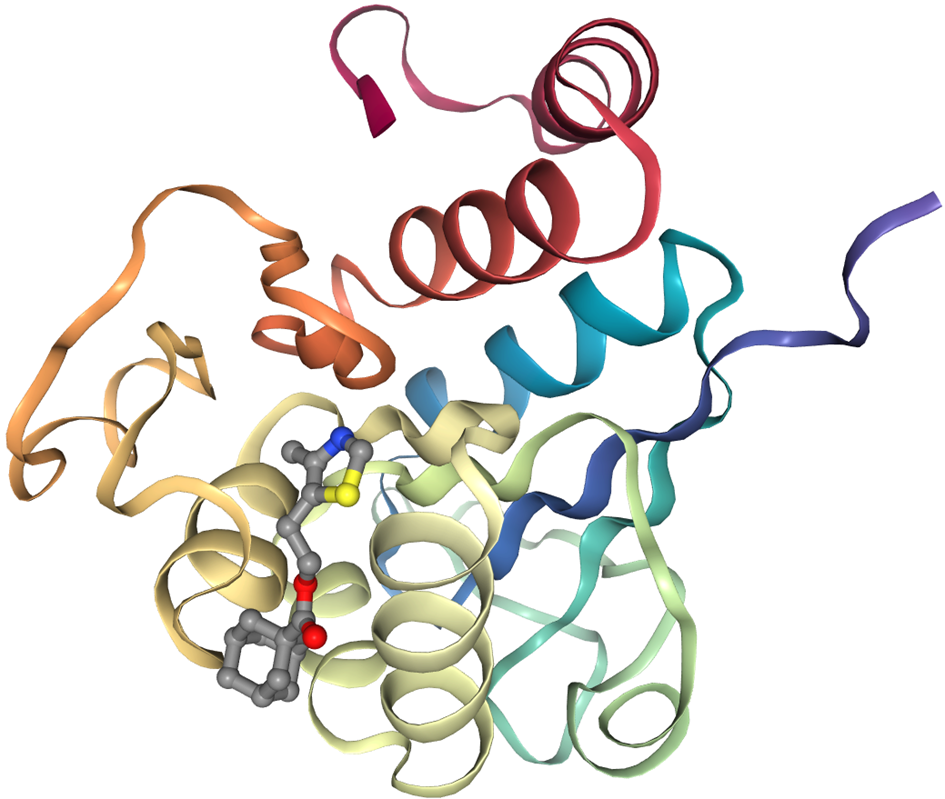
\includegraphics[width=\linewidth]{protein-ligand}

    \pagebreak

    \tableofcontents


    \section{Kurzfassung}\label{sec:kurzfassung}



    Tropenkrankheiten stellen in ihren Verbeitungsgebieten eine extreme Bedrohung für die dortige Bevölkerung dar. Gemessen an ihrer Bedeutung - Malaria ist z. B. mit 200 Millionen Fällen pro Jahr die häufigste Infektionskrankheit der Welt  - erfahren sie in nicht betroffenen Industrieländern nur wenig Aufmerksamkeit in Medien, in Form von Forschungsprojekten und in den Entwicklungsabteilungen von Pharmafirmen.

    Aufgrund der Veröffentlichung des AlphaFold-Papers im Juli 2021 und der gleichzeitig veröffentlichten Datenbank von dreidimensionalen Proteinmodellen, sowie dem UseGalaxy-Server der Universität Freiburg haben wir gute Voraussetzungen bekommen, um mithilfe von Protein-Liganden-Docking nach möglichen Wirkstoffen gegen Tropenkrankheiten zu suchen.


% \section{Inhaltsverzeichnis}
% \tableofcontents


    \section{Einleitung}\label{sec:einleitung}


        \begin{wrapfigure}{r}{0.3\textwidth}
            
\includegraphics[width=\linewidth]{Galaxy-logo}
            \caption{Logo von Galaxy Europe}
        \end{wrapfigure}

        Tropenkrankheiten stellen in Entwicklungsländern verheerende Schäden an und fordern viele Opfer ein. So ist z.B. Malaria mit 200 Millionen Fällen pro Jahr die häufigste Infektionskrankheit der Welt. Trotz der massiven Schäden, die Tropenkrankheiten, wie z.B. Malaria, die Afrikanische Schlafkrankheit und Hepatitis A- anrichten, schenken Industrieländer und die dort hiesigen Pharmakonzerne diesen Bedrohungen nur wenig Beachtung. Die Entwicklung und der Verkauf von Medikamenten gegen diese weit verbreiteten Krankheiten erschien den Konzernen als nicht lukrativ genug, obwohl der Markt dafür vorhanden wäre und wurde demnach vernachlässigt. (Doch mittlerweile gibt es Vereinigungen, die gegen diese reale Gefahr kämpfen. Wir möchten uns dem anschließen.)  Nun versuchen wir mit unserem Projekt mithilfe von Bioinformatik (weitere) helfende Arzneimittel zu finden und unter Umständen auch eine neue Entdeckung zu machen. Da uns keine Laborforschungsmittel oder Supercomputer zur Verfügung stehen, müssen wir auf öffentlich zugängliche Ressourcen zurückgreifen. Hierfür gibt es die webbasierte Plattform für Computational Science, mit Fokus auf Biologie, namens „Galaxy“. Damit kann man selbstverständlich kein fertiges Medikament entwickeln, dennoch erhoffen wir uns damit eine Grundlage für weitere Forschung zu schaffen. Dort versuchen wir mithilfe der zur Verfügung gestellten Werkzeuge Protein-Liganden- Docking zu simulieren und damit einen wirkungsvollen Stoff gegen die Krankheiten zu finden. Doch was genau ist dieses Protein-Liganden-Docking? Dieses Verfahren ist eine „molecular modelling“- Technik, wobei mittels Bioinformatik versucht wird herauszufinden, welche Liganden mit welchen Proteinen an welcher Stelle binden. Man benötigt dementsprechend Daten über den Liganden und den Rezeptor des Proteins. Jetzt hat dieses Verfahren eine pharmazeutische Bedeutung, da man zum einen mögliche Wirkstoffe finden kann, die vitale Proteine des Krankheitserregers außer Kraft setzen können. Weiter erleichtert es auch die Suche, da das Auswahlverfahren nun „in silico“ erfolgen kann und nicht alle möglichen Kandidaten im Labor getestet werden müssen.

    Auch wir möchten dieses bioinformatische Verfahren anwenden. Doch warum haben wir ausgerechnet diese Krankheiten gewählt?

        \begin{wrapfigure}{r}{0.3\textwidth}
            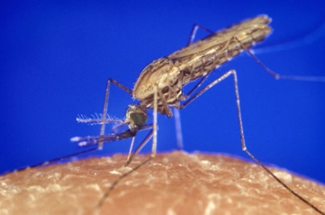
\includegraphics[width=\linewidth]{Anophelesmucke}
            \caption{Die Anophelesmücke beim Blutsaugen CDC/James Gathany}
        \end{wrapfigure}
        Malaria ist eine vor allem in den tropischen Regionen Afrikas anzutreffen, aber auch in Südostasien und in den nördlichen Teilen Südamerikas zu finden. Wie bereits erwähnt ist Malaria, auch Sumpf- oder Tropenfieber bekannt, die häufigste Tropenkrankheit. Der wichtigste Überträger der Krankheit ist die weibliche Anophelesmücke. Malaria kann Symptome wie Fieber, Erbrechen, Gelbsucht und Krämpfe umfassen. Vor allem die von uns gewählte Variante der Falciparum-Malaria ruft schwere Symptome wie Lähmung oder Koma hervor. Über Lungen- oder Nierenversagen führt die Krankheit zum Tod.

        \begin{wrapfigure}{r}{0.3\textwidth}
            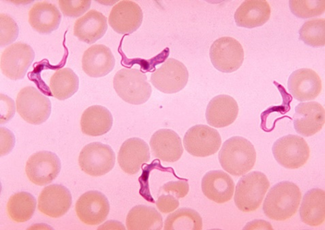
\includegraphics[width=\linewidth]{Trypanosoma}
            \caption{Trypanosoma, die Erreger der Schlafkrankheit (CDC/Dr. Myron G. Schultz)}
        \end{wrapfigure}
        Ebenfalls eine durch ein Insekt verbreitete Krankheit ist die Afrikanische Trypanosomiasis, oder auch Afrikanische Schlafkrankheit, dessen Erreger Trypanosoma brucei durch die Tsetse-Fliege übertragen wird. Man kann aktuell mit ca. 500 000 Betroffenen in Afrika rechnen. Über Fieber, Gliederschmerzen, Lymphknotenschwellung und Anämie führt die Krankheit zum namengebenden Dämmerzustand und anschließend zum Tod.

    Als dritte Krankheit betrachten wir die Chagas-Krankheit, auch Südamerikanische Trypanosomiasis genannt. Der Erreger Trypanosoma cruci, ein Verwandter der Trypanosoma brucei, wird durch den Kot verschiedener Raubwanzen, aber vor allem von Triatoma infestans, übertragen. Aktuell gibt es ca. 18 Millionen Erkrankte, wobei jedes Jahr 50.000 dazukommen. Zahl der Todesfälle beträgt jährlich um die 15.000. Die Krankheit verursacht Ödeme, chronisches Herzversagen und dem Absterben von Nervenzellen im Darm. Dies führt mitunter zum Tod durch Darmverschluss oder Darmdurchbruch.

    Sowohl die Chagas-Krankheit als auch die Afrikanische Trypanosomiasis sind von der Weltgesundheitsorganisation als „neglected tropical diseases“ (NTD´s) anerkannt.

        \begin{wrapfigure}{r}{0.3\textwidth}
            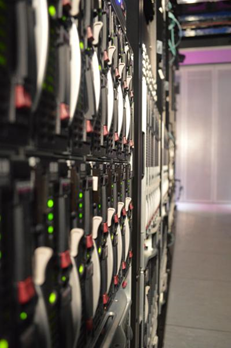
\includegraphics[width=\linewidth]{Datacenter}
            \caption{Datencenter des EMBL-EBI (EMBL-EBI)}
        \end{wrapfigure}

        Mit Galaxy haben wir schon eine gute Grundlage zur Erforschung und Durchführung des Protein-Liganden-Dockings, jedoch fehlen uns die Daten über den Arzneistoff, also den Liganden, und das Organell, sprich ein vitales Protein, welches im Erreger außer Kraft gesetzt werden soll, sodass er stirbt. Man benötigt also Datenbanken, mit den entsprechenden Sequenzen bzw. Strukturen. Für das Protein gibt es die die Proteinstrukturdatenbank AlphaFold, welches von DeepMind und EMBL-EBI entwickelt wurde. Da werden Proteinstrukturen aufgeführt, die von einer AI auf Grundlage der Aminosäuresequenz ermittelt bzw. vorhergesagt wurden. Dabei sind diese Vorhersagen sehr präzise. Hat man dann eine mögliche Struktur für den Liganden gefunden, kann man nach realen Chemikalien in der EMBL-EBI Datenbank suchen. Das „European Molecular Biology Laboratory Bioinformatics Institute“ beherbergt die größte öffentlich zugängliche biologische Datenbank und bietet gleichzeitig auch bioinformatische Dienste für Forschende aus aller Welt an. Nur mithilfe von Galaxy, AlphaFold und EMBL-EBI können wir an unserem Projekt forschen. Und wie genau das abläuft wird im weiteren Verlauf erläutert.


    \section{Vorgehensweise, Materialien und Methode}\label{sec:vorgehensweise-materialien-und-methode}

    \subsection{Vorbereitung}\label{subsec:vorbereitung}

    \subsubsection{Krankheiten wählen}

    \subsubsection{Proteine und natürliche Liganden finden}

    \paragraph{Malaria}

    \subparagraph{Protein}

    \subparagraph{Ligand}

    \paragraph{Afrikanische Schlafkrankheit}

    \paragraph{Chagas-Krankheit}

    \subsection{Docking mit Galaxy}\label{subsec:galaxy}

    \subsubsection{Übersicht}

    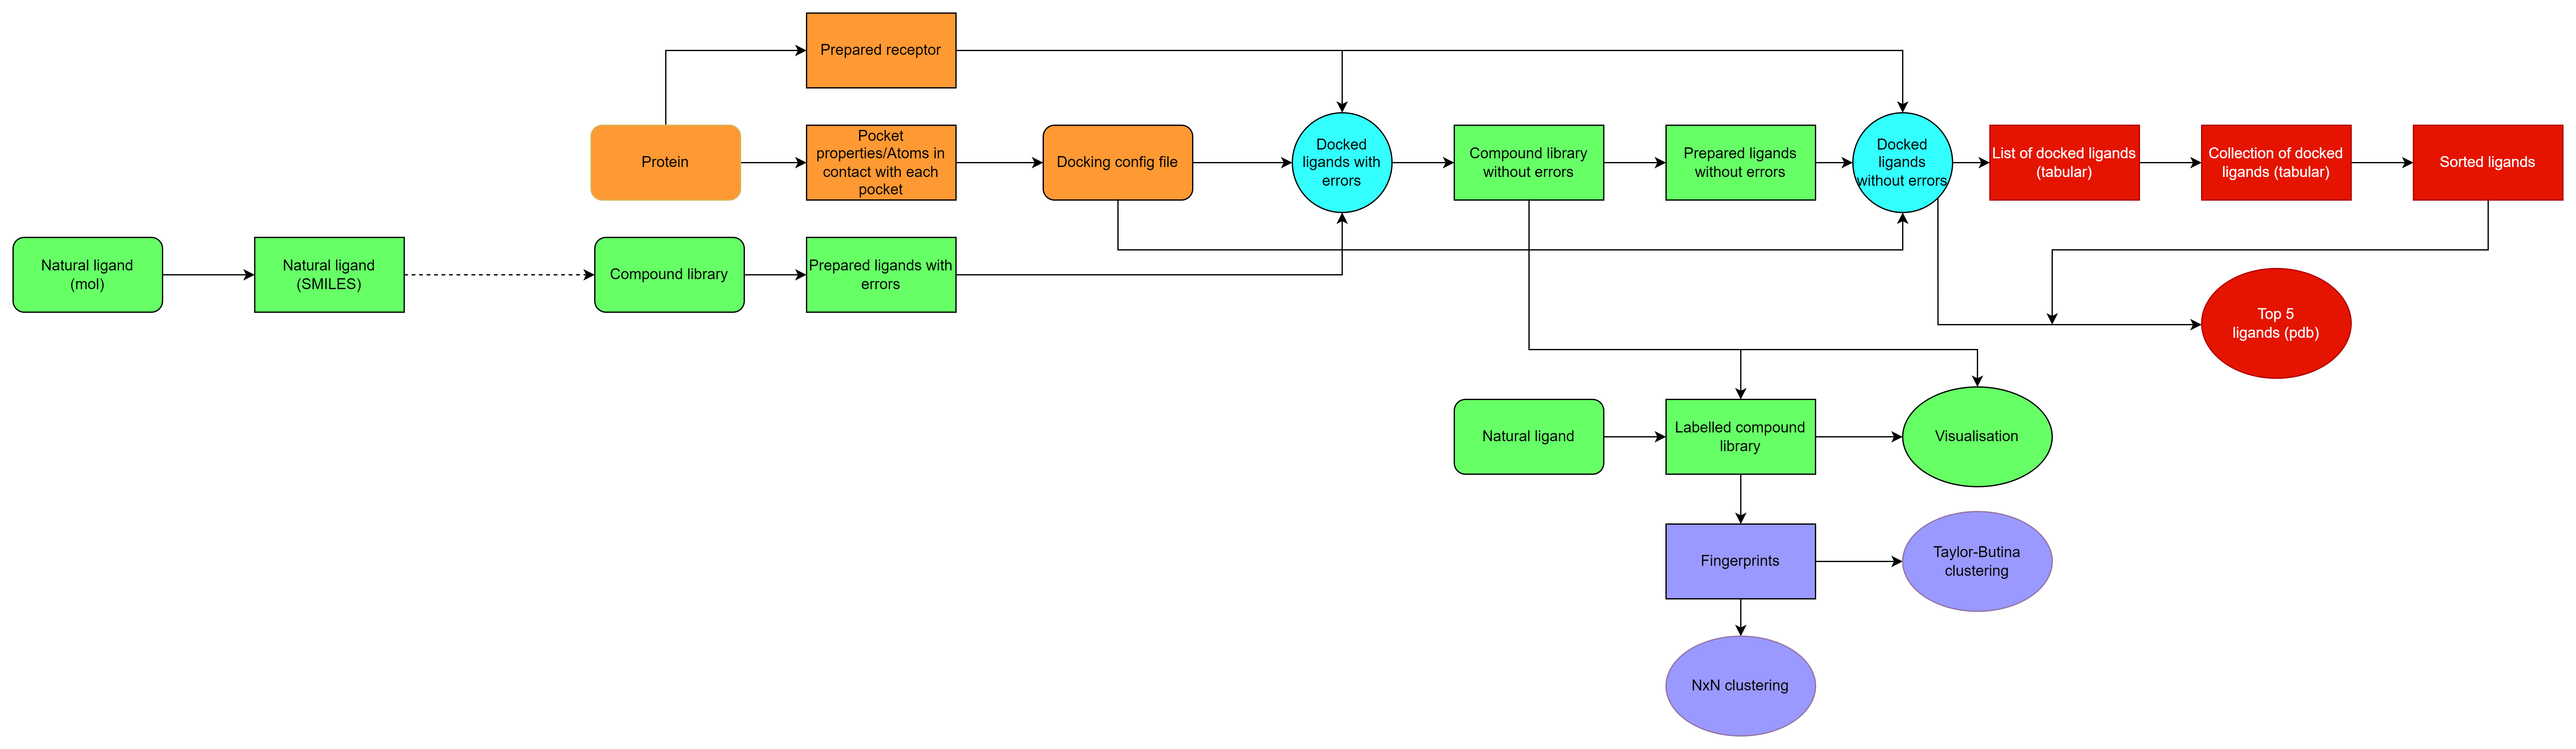
\includegraphics[width=\linewidth]{flowchart_Plasmodium Falciparum}
    \caption{Docking mit Plasmodium Falciparum (Malaria)}

    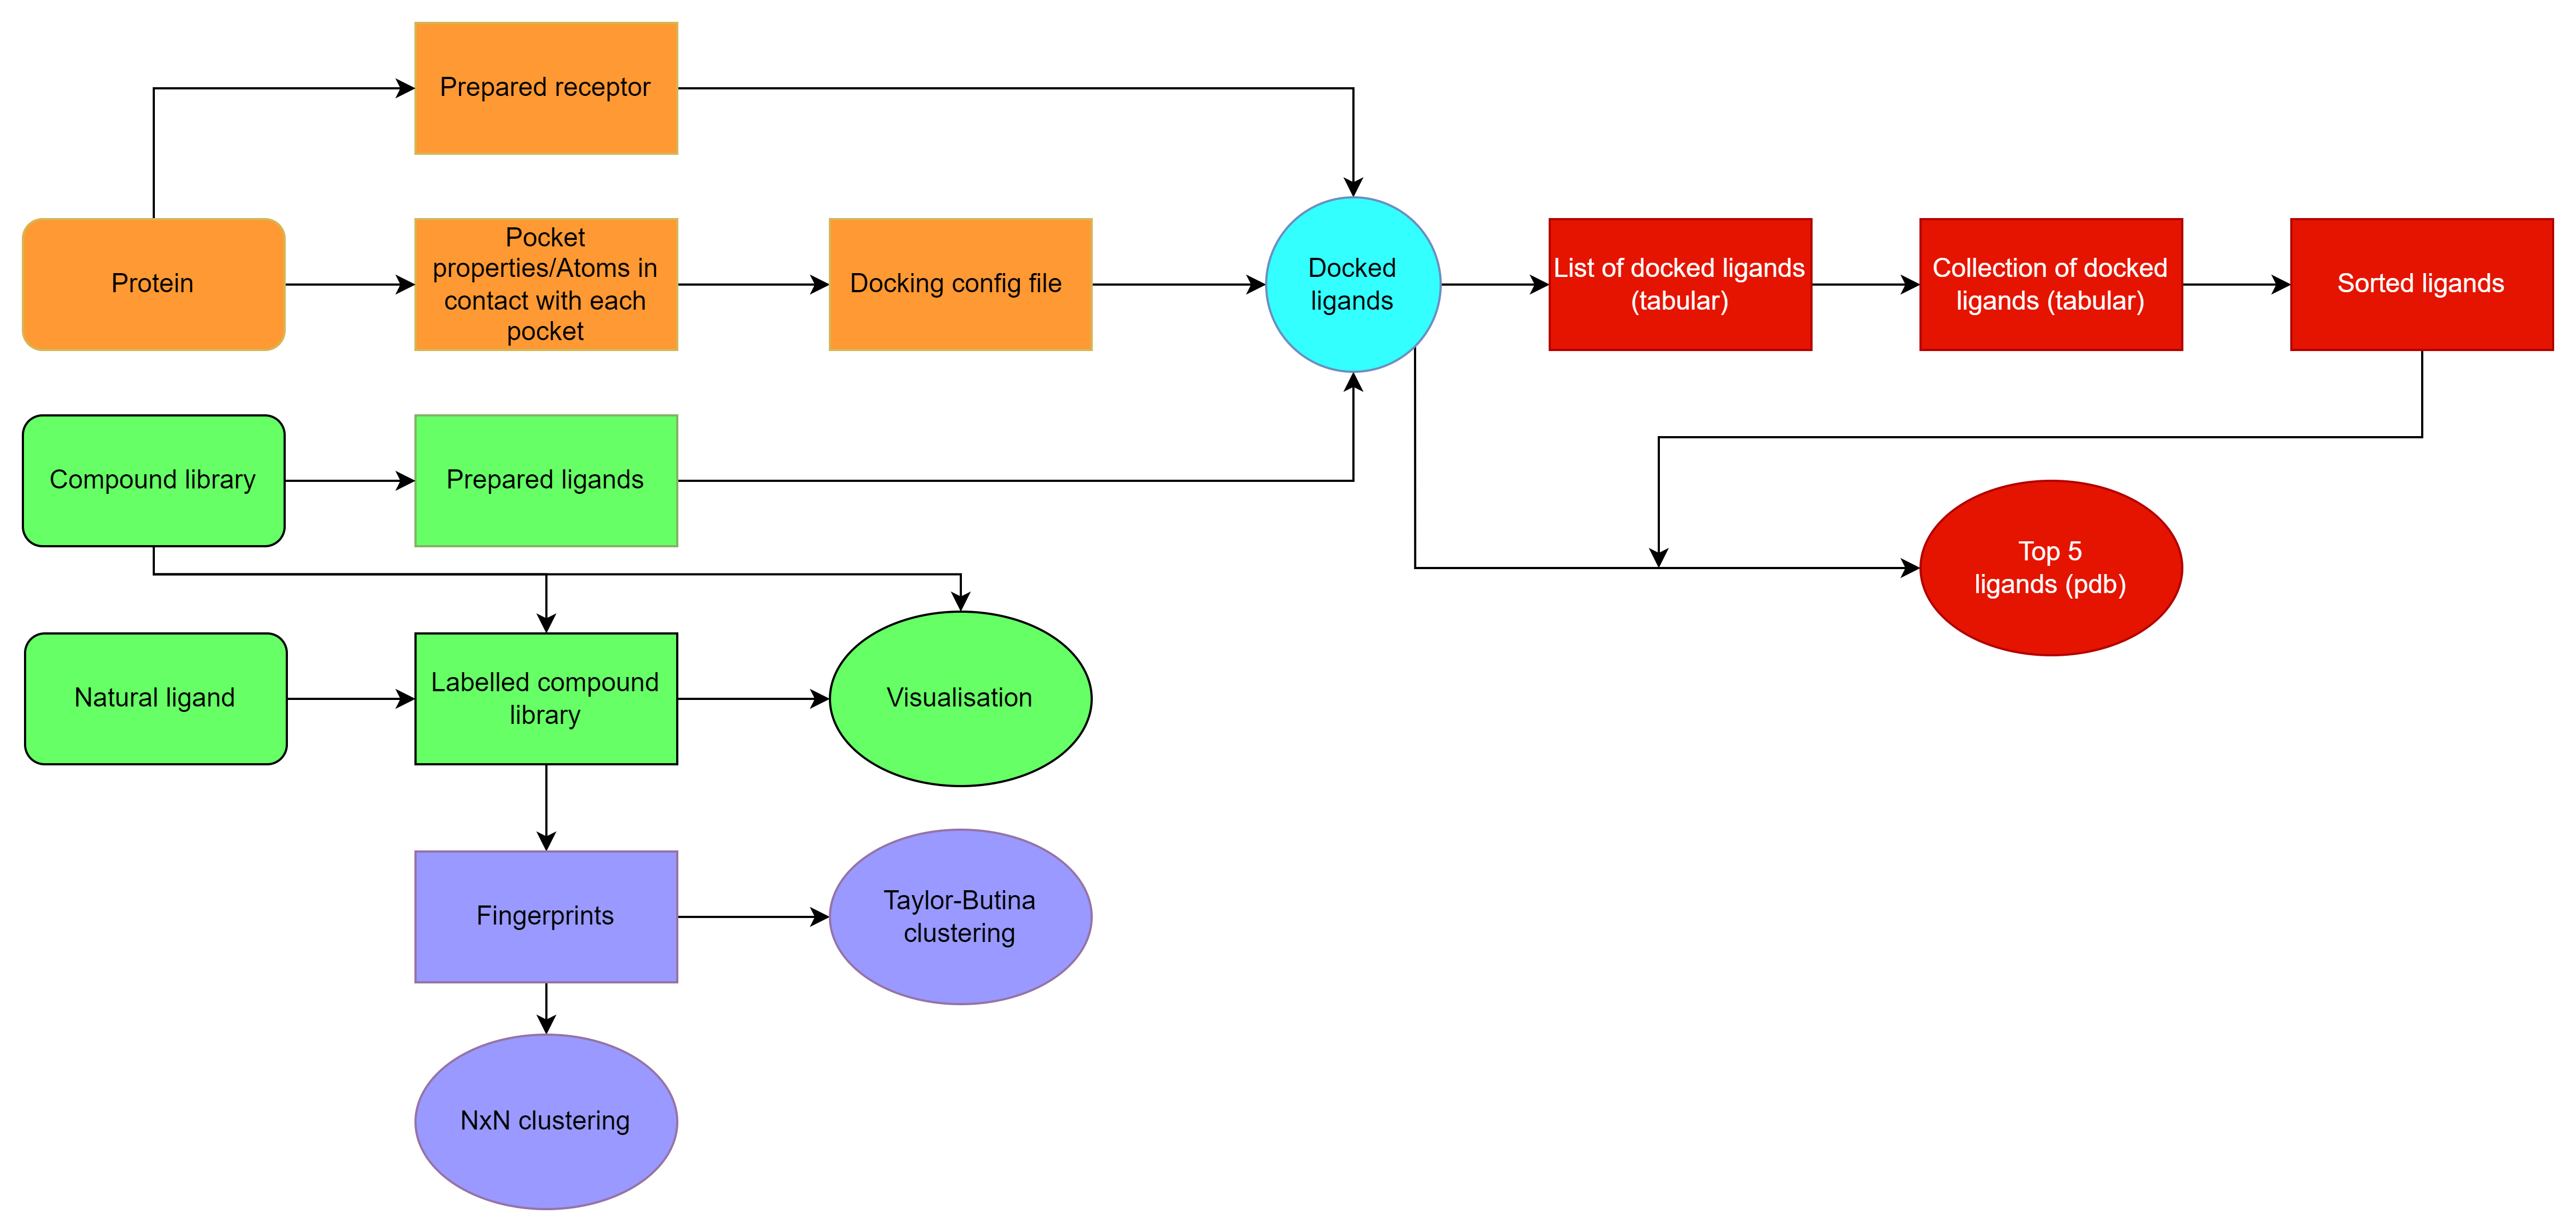
\includegraphics[width=\linewidth]{flowchart_Trypanosoma brucei gambiense}
    \caption{Docking mit Trypanosoma brucei gambiense (Afrikanische Schlafkrankheit)}

    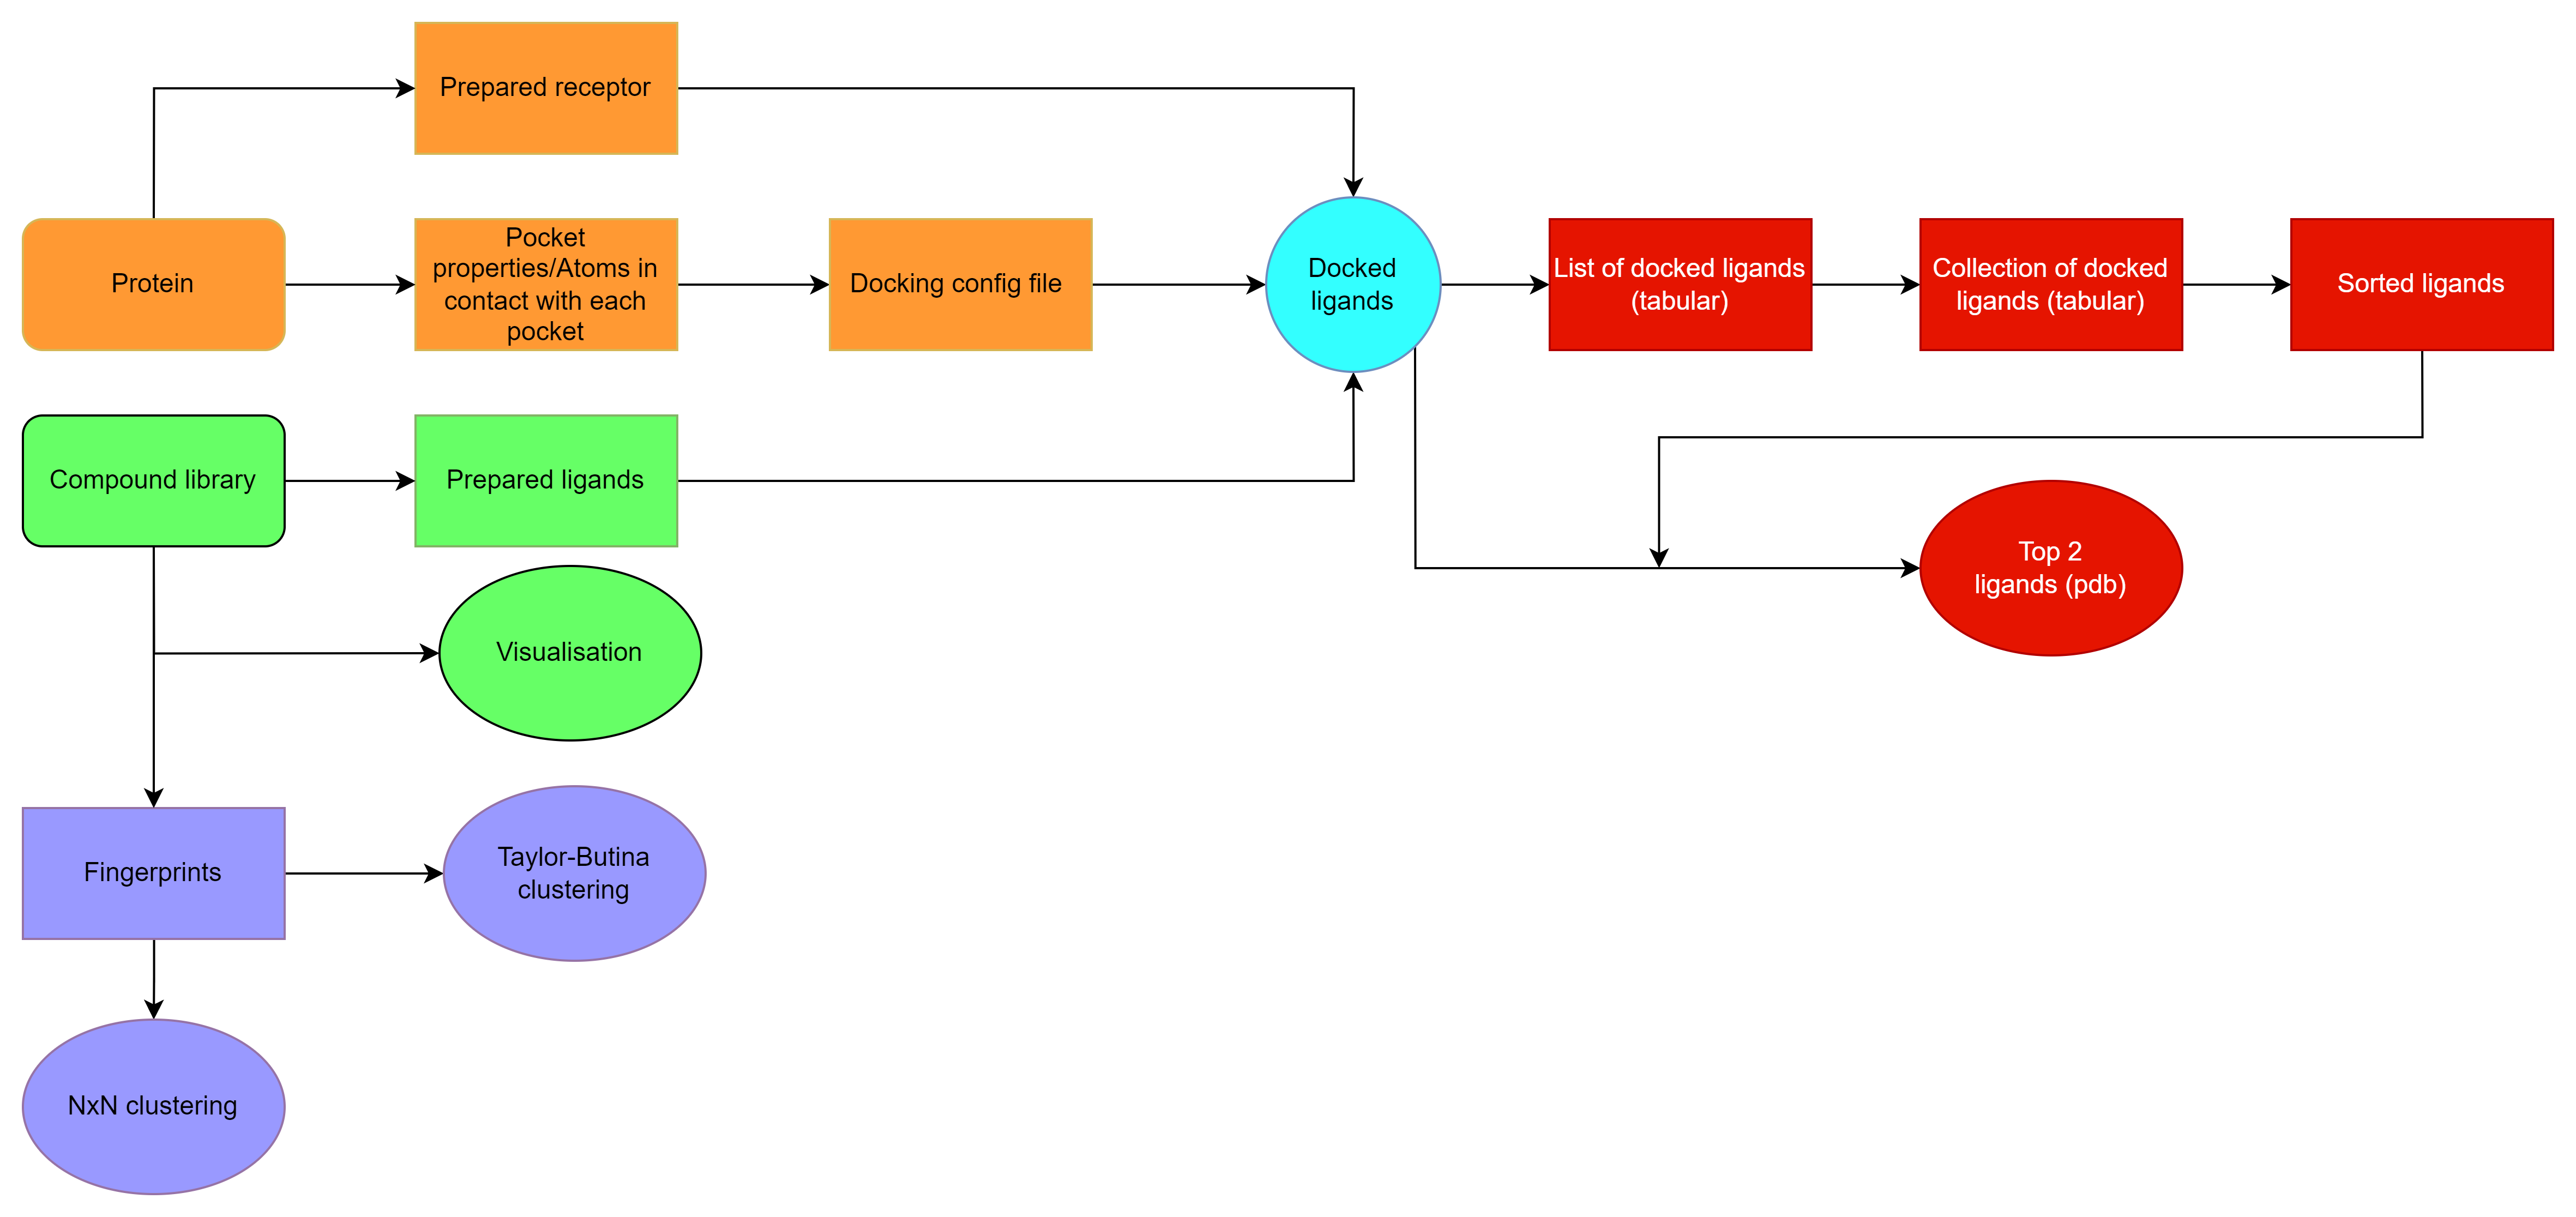
\includegraphics[width=\linewidth]{flowchart_Trypanosoma cruzi}
    \caption{Docking mit Trypanosoma cruzi (Chagas-Karankheit)}

    \subsubsection{Protein- und Ligandenstruktur eingeben}\label{subsec:protein--und-ligandenstruktur-eingeben}

    Auf der Galaxy-Website kann man ein neues Programm (History genannt) erstellen. Danach luden wir in der History als erstes über den „Upload-Data“-Button die PDB -Datei des Pro-teins Plasmodium Falciparum von unserem lokalen PC hoch.

    SMILES-String-Herkunft erklären!!!

    Dann brauchten wir eine Compound library, in welcher Moleküle aufgelistet sein sollten, die dem Molekül des natürlichen Liganden vom Plasmodium Falciparum ähnelten. Diese erstellten wir, indem wir das auf Galaxy bereitstehende Tool „Search ChEMBL database“ nutzten. Die-ses Tool ermöglicht es, die ChEMBL-Datenbank mit Hilfe des Tanimoto-Algorithmus nach Molekülen zu durchsuchen, die ähnlich zu einem Molekül sind, dass man über einen einzuge-benden SMILES-String übermittelt. Wir gaben also den SMILES-String \texttt{(c1(c(ncs1)C)CCO)} des natürlichen Liganden (5-(2-hydroxyethyl)-4-methylthiazole) als SMILES-Input eingegeben.
    In dem Tool konnte man auswählen, wie hoch der „Tanimoto cutoff score“ sein soll. Dieser Score entscheidet, wie hoch die Ähnlichkeit zwischen einem Liganden aus der Datenbank und dem eingegeben Vergleichs-Liganden sein muss, um in die Compound library aufgenommen zu werden. Ein Bereich von 40 (niedrige Ähnlichkeit ist ausreichend) bis 100 steht zur Verfü-gung Außerdem haben wir ausgewählt, dass der „Filter for Lipinski‘s Rule of Five“ ange-wendet werden soll. Die Rule of Five ist eine Faustregel, die Moleküle auf ihre orale Biover-fügbarkeit überprüft, also auf die Frage, ob ein Molekül prinzipiell als oral-einzunehmendes Arzneimittel geeignet wäre.
    Evt. einzelne Kriterien und Entwickler nennen.
    Nach dem Ausführen dieses Befehls haben wir nun also eine Compound library im Format einer SMILES-Liste, die aus in diesem Fall 50 Molekülen besteht, die dem natürlichen Ligan-den des Plasmodium Falciparums ähnlich sind und außerdem als Arzneimittel theoretisch ge-eignet wären. Die Datei sieht folgendermaßen aus: In jeder Zeile ist ein Molekül aufgelistet, zunächst mit dem SMILES-String und dann mit dem Titel, also der ChEMBL-ID des jeweili-gen Moleküls.

    %\begin{footnotesize}
        \begin{figure}
            \centering
            \def\svgwidth{\columnwidth}
            \documentclass{article}
\usepackage{amsmath}
\usepackage{color,pxfonts,fix-cm}
\usepackage{latexsym}
\usepackage[mathletters]{ucs}
\usepackage[T1]{fontenc}
\usepackage[utf8x]{inputenc}
\usepackage{pict2e}
\usepackage{wasysym}
\usepackage[english]{babel}
\usepackage{tikz}
\pagestyle{empty}
\usepackage[margin=0in,paperwidth=75pt,paperheight=65pt]{geometry}
\begin{document}
\definecolor{color_283006}{rgb}{1,1,1}
\definecolor{color_29791}{rgb}{0,0,0}
\definecolor{color_41950}{rgb}{0.047059,0.047059,1}
\definecolor{color_275230}{rgb}{1,0.047059,0.047059}
\definecolor{color_157611}{rgb}{0.498039,0.698039,1}
\definecolor{color_206367}{rgb}{0.698039,0.698039,0}
\begin{tikzpicture}[overlay]
\path(0pt,0pt);
\filldraw[color_283006][nonzero rule]
(-15pt, 10.25pt) -- (60pt, 10.25pt)
 -- (60pt, 10.25pt)
 -- (60pt, -55pt)
 -- (60pt, -55pt)
 -- (-15pt, -55pt) -- cycle
;
\filldraw[color_29791][nonzero rule]
(-11.277pt, 8.762001pt) -- (-11.609pt, 8.183998pt)
;
\draw[color_29791,line width=0.051199pt]
(-11.277pt, 8.762001pt) -- (-11.609pt, 8.183998pt)
;
\draw[color_29791,line width=0.051199pt,line cap=round,miter limit=4]
(-11.609pt, 8.105pt) -- (-12.277pt, 8.105pt)
;
\draw[color_29791,line width=0.051199pt,line cap=round,miter limit=4]
(-11.609pt, 8.262001pt) -- (-12.277pt, 8.262001pt)
;
\filldraw[color_29791][nonzero rule]
(-11.609pt, 8.183998pt) -- (-11.113pt, 7.32pt)
;
\draw[color_29791,line width=0.051199pt]
(-11.609pt, 8.183998pt) -- (-11.113pt, 7.32pt)
;
\filldraw[color_29791][nonzero rule]
(-10.113pt, 5.59pt) -- (-9.535pt, 5.254002pt)
;
\draw[color_29791,line width=0.051199pt]
(-10.113pt, 5.59pt) -- (-9.535pt, 5.254002pt)
;
\filldraw[color_29791][nonzero rule]
(-8.34pt, 2.655998pt) -- (-7.746pt, 2.308998pt)
;
\draw[color_29791,line width=0.051199pt]
(-8.34pt, 2.655998pt) -- (-7.746pt, 2.308998pt)
;
\filldraw[color_29791][nonzero rule]
(-8.418pt, 2.52pt) -- (-7.82pt, 2.175999pt)
;
\draw[color_29791,line width=0.051199pt]
(-8.418pt, 2.52pt) -- (-7.82pt, 2.175999pt)
;
\draw[color_29791,line width=0.051199pt,line cap=round,miter limit=4]
(-11.609pt, 6.452999pt) -- (-12.277pt, 6.452999pt)
;
\filldraw[color_29791][nonzero rule]
(-12.777pt, 6.164001pt) -- (-13.109pt, 5.59pt)
;
\draw[color_29791,line width=0.051199pt]
(-12.777pt, 6.164001pt) -- (-13.109pt, 5.59pt)
;
\filldraw[color_29791][nonzero rule]
(-8.379pt, 3.59pt) -- (-7.516pt, 5.085999pt)
;
\draw[color_29791,line width=0.051199pt]
(-8.379pt, 3.59pt) -- (-7.516pt, 5.085999pt)
;
\filldraw[color_29791][nonzero rule]
(-7.516pt, 5.085999pt) -- (-8.379pt, 5.59pt)
;
\draw[color_29791,line width=0.051199pt]
(-7.516pt, 5.085999pt) -- (-8.379pt, 5.59pt)
;
\filldraw[color_29791][nonzero rule]
(-7.738pt, 5.004002pt) -- (-8.34pt, 5.352001pt)
;
\draw[color_29791,line width=0.051199pt]
(-7.738pt, 5.004002pt) -- (-8.34pt, 5.352001pt)
;
\filldraw[color_29791][nonzero rule]
(-8.379pt, 5.59pt) -- (-8.957pt, 5.254002pt)
;
\draw[color_29791,line width=0.051199pt]
(-8.379pt, 5.59pt) -- (-8.957pt, 5.254002pt)
;
\draw[color_29791,line width=0.051199pt,line cap=round,miter limit=4]
(-9.246pt, 4.754002pt) -- (-9.246pt, 4.09pt)
;
\filldraw[color_29791][nonzero rule]
(-9.246pt, 4.09pt) -- (-8.379pt, 3.59pt)
;
\draw[color_29791,line width=0.051199pt]
(-9.246pt, 4.09pt) -- (-8.379pt, 3.59pt)
;
\filldraw[color_29791][nonzero rule]
(-9.023pt, 4.167999pt) -- (-8.422pt, 3.824001pt)
;
\draw[color_29791,line width=0.051199pt]
(-9.023pt, 4.167999pt) -- (-8.422pt, 3.824001pt)
;
\filldraw[color_29791][nonzero rule]
(-9.609pt, 6.452999pt) -- (-10.113pt, 5.59pt)
;
\draw[color_29791,line width=0.051199pt]
(-9.609pt, 6.452999pt) -- (-10.113pt, 5.59pt)
;
\draw[color_29791,line width=0.051199pt,line cap=round,miter limit=4]
(-10.113pt, 5.59pt) -- (-11.113pt, 5.59pt)
;
\draw[color_29791,line width=0.051199pt,line cap=round,miter limit=4]
(-10.266pt, 5.772999pt) -- (-10.957pt, 5.772999pt)
;
\filldraw[color_29791][nonzero rule]
(-11.113pt, 5.59pt) -- (-11.609pt, 6.452999pt)
;
\draw[color_29791,line width=0.051199pt]
(-11.113pt, 5.59pt) -- (-11.609pt, 6.452999pt)
;
\filldraw[color_29791][nonzero rule]
(-11.609pt, 6.452999pt) -- (-11.113pt, 7.32pt)
;
\draw[color_29791,line width=0.051199pt]
(-11.609pt, 6.452999pt) -- (-11.113pt, 7.32pt)
;
\filldraw[color_29791][nonzero rule]
(-11.375pt, 6.495998pt) -- (-11.031pt, 7.094002pt)
;
\draw[color_29791,line width=0.051199pt]
(-11.375pt, 6.495998pt) -- (-11.031pt, 7.094002pt)
;
\draw[color_29791,line width=0.051199pt,line cap=round,miter limit=4]
(-11.113pt, 7.32pt) -- (-10.113pt, 7.32pt)
;
\filldraw[color_29791][nonzero rule]
(-10.113pt, 7.32pt) -- (-9.609pt, 6.452999pt)
;
\draw[color_29791,line width=0.051199pt]
(-10.113pt, 7.32pt) -- (-9.609pt, 6.452999pt)
;
\filldraw[color_29791][nonzero rule]
(-10.195pt, 7.094002pt) -- (-9.848pt, 6.495998pt)
;
\draw[color_29791,line width=0.051199pt]
(-10.195pt, 7.094002pt) -- (-9.848pt, 6.495998pt)
;
\filldraw[color_29791][nonzero rule]
(-7.516pt, 7.09pt) -- (-8.379pt, 6.585999pt)
;
\draw[color_29791,line width=0.051199pt]
(-7.516pt, 7.09pt) -- (-8.379pt, 6.585999pt)
;
\filldraw[color_29791][nonzero rule]
(-7.555pt, 6.852001pt) -- (-8.156pt, 6.504002pt)
;
\draw[color_29791,line width=0.051199pt]
(-7.555pt, 6.852001pt) -- (-8.156pt, 6.504002pt)
;
\draw[color_29791,line width=0.051199pt,line cap=round,miter limit=4]
(-8.379pt, 6.585999pt) -- (-8.379pt, 5.59pt)
;
\filldraw[color_29791][nonzero rule]
(-7.516pt, 5.085999pt) -- (-6.648pt, 5.59pt)
;
\draw[color_29791,line width=0.051199pt]
(-7.516pt, 5.085999pt) -- (-6.648pt, 5.59pt)
;
\draw[color_29791,line width=0.051199pt,line cap=round,miter limit=4]
(-6.648pt, 5.59pt) -- (-6.648pt, 6.585999pt)
;
\draw[color_29791,line width=0.051199pt,line cap=round,miter limit=4]
(-6.832pt, 5.742001pt) -- (-6.832pt, 6.433998pt)
;
\filldraw[color_29791][nonzero rule]
(-6.648pt, 6.585999pt) -- (-7.516pt, 7.09pt)
;
\draw[color_29791,line width=0.051199pt]
(-6.648pt, 6.585999pt) -- (-7.516pt, 7.09pt)
;
\filldraw[color_29791][nonzero rule]
(-13.977pt, 5.085999pt) -- (-13.109pt, 5.59pt)
;
\draw[color_29791,line width=0.051199pt]
(-13.977pt, 5.085999pt) -- (-13.109pt, 5.59pt)
;
\draw[color_29791,line width=0.051199pt,line cap=round,miter limit=4]
(-13.109pt, 5.59pt) -- (-13.109pt, 4.585999pt)
;
\filldraw[color_29791][nonzero rule]
(-13.109pt, 4.585999pt) -- (-13.977pt, 5.085999pt)
;
\draw[color_29791,line width=0.051199pt]
(-13.109pt, 4.585999pt) -- (-13.977pt, 5.085999pt)
;
\filldraw[color_29791][nonzero rule]
(-10.113pt, 2.585999pt) -- (-9.246pt, 2.09pt)
;
\draw[color_29791,line width=0.051199pt]
(-10.113pt, 2.585999pt) -- (-9.246pt, 2.09pt)
;
\filldraw[color_29791][nonzero rule]
(-9.246pt, 2.09pt) -- (-8.379pt, 2.585999pt)
;
\draw[color_29791,line width=0.051199pt]
(-9.246pt, 2.09pt) -- (-8.379pt, 2.585999pt)
;
\draw[color_29791,line width=0.051199pt,line cap=round,miter limit=4]
(-8.379pt, 2.585999pt) -- (-8.379pt, 3.59pt)
;
\filldraw[color_29791][nonzero rule]
(-9.246pt, 4.09pt) -- (-10.113pt, 3.59pt)
;
\draw[color_29791,line width=0.051199pt]
(-9.246pt, 4.09pt) -- (-10.113pt, 3.59pt)
;
\draw[color_29791,line width=0.051199pt,line cap=round,miter limit=4]
(-10.113pt, 3.59pt) -- (-10.113pt, 2.585999pt)
;
\end{tikzpicture}
\begin{picture}(-5,0)(2.5,0)
\put(-12.76437,6.247742){\fontsize{0}{1}\usefont{T1}{ptm}{m}{n}\selectfont\color{color_41950}N}
\put(-12.76437,6.657337){\fontsize{0}{1}\usefont{T1}{ptm}{m}{n}\selectfont\color{color_41950}H}
\put(-7.647624,1.871071){\fontsize{0}{1}\usefont{T1}{ptm}{m}{n}\selectfont\color{color_275230}O}
\put(-11.21404,8.844322){\fontsize{0}{1}\usefont{T1}{ptm}{m}{n}\selectfont\color{color_41950}NH}
\put(-10.59965,8.750118){\fontsize{0}{1}\usefont{T1}{ptm}{m}{n}\selectfont\color{color_41950}2}
\put(-9.400284,4.882504){\fontsize{0}{1}\usefont{T1}{ptm}{m}{n}\selectfont\color{color_41950}N}
\put(-12.76437,7.978798){\fontsize{0}{1}\usefont{T1}{ptm}{m}{n}\selectfont\color{color_275230}O}
\put(-12.55728,1.089287){\fontsize{0}{1}\usefont{T1}{ptm}{m}{n}\selectfont\color{color_29791}CHEMBL410053}
\end{picture}
\begin{tikzpicture}[overlay]
\path(0pt,0pt);
\filldraw[color_29791][nonzero rule]
(-3.395pt, 2.812pt) -- (-2.801pt, 3.547001pt)
;
\draw[color_29791,line width=0.047271pt]
(-3.395pt, 2.812pt) -- (-2.801pt, 3.547001pt)
;
\filldraw[color_29791][nonzero rule]
(-1.219pt, 4.460999pt) -- (-0.602pt, 4.625pt)
;
\draw[color_29791,line width=0.047271pt]
(-1.219pt, 4.460999pt) -- (-0.602pt, 4.625pt)
;
\filldraw[color_29791][nonzero rule]
(1.223pt, 5.117001pt) -- (2.136999pt, 5.359001pt)
;
\draw[color_29791,line width=0.047271pt]
(1.223pt, 5.117001pt) -- (2.136999pt, 5.359001pt)
;
\filldraw[color_29791][nonzero rule]
(2.136999pt, 5.359001pt) -- (2.301001pt, 5.977001pt)
;
\draw[color_29791,line width=0.047271pt]
(2.136999pt, 5.359001pt) -- (2.301001pt, 5.977001pt)
;
\filldraw[color_29791][nonzero rule]
(2.188pt, 5.41pt) -- (2.636999pt, 4.960999pt)
;
\draw[color_29791,line width=0.047271pt]
(2.188pt, 5.41pt) -- (2.636999pt, 4.960999pt)
;
\filldraw[color_29791][nonzero rule]
(2.086pt, 5.308998pt) -- (2.535pt, 4.859001pt)
;
\draw[color_29791,line width=0.047271pt]
(2.086pt, 5.308998pt) -- (2.535pt, 4.859001pt)
;
\filldraw[color_29791][nonzero rule]
(0.555pt, 5.785pt) -- (0.719pt, 6.402pt)
;
\draw[color_29791,line width=0.047271pt]
(0.555pt, 5.785pt) -- (0.719pt, 6.402pt)
;
\filldraw[color_29791][nonzero rule]
(0.582pt, 6.914001pt) -- (0.129pt, 7.367001pt)
;
\draw[color_29791,line width=0.047271pt]
(0.582pt, 6.914001pt) -- (0.129pt, 7.367001pt)
;
\filldraw[color_29791][nonzero rule]
(-3.848pt, 4.832001pt) -- (-4.383pt, 4.484001pt)
;
\draw[color_29791,line width=0.047271pt]
(-3.848pt, 4.832001pt) -- (-4.383pt, 4.484001pt)
;
\filldraw[color_29791][nonzero rule]
(-3.926pt, 4.949001pt) -- (-4.461pt, 4.602001pt)
;
\draw[color_29791,line width=0.047271pt]
(-3.926pt, 4.949001pt) -- (-4.461pt, 4.602001pt)
;
\filldraw[color_29791][nonzero rule]
(-3.145pt, 6.348pt) -- (-3.66pt, 7.145pt)
;
\draw[color_29791,line width=0.047271pt]
(-3.145pt, 6.348pt) -- (-3.66pt, 7.145pt)
;
\filldraw[color_29791][nonzero rule]
(-3.145pt, 6.348pt) -- (-2.715pt, 7.191002pt)
;
\draw[color_29791,line width=0.047271pt]
(-3.145pt, 6.348pt) -- (-2.715pt, 7.191002pt)
;
\filldraw[color_29791][nonzero rule]
(-1.758pt, 4.574001pt) -- (-2.254pt, 4.977001pt)
;
\draw[color_29791,line width=0.047271pt]
(-1.758pt, 4.574001pt) -- (-2.254pt, 4.977001pt)
;
\filldraw[color_29791][nonzero rule]
(-2.254pt, 4.977001pt) -- (-3.043pt, 4.460999pt)
;
\draw[color_29791,line width=0.047271pt]
(-2.254pt, 4.977001pt) -- (-3.043pt, 4.460999pt)
;
\filldraw[color_29791][nonzero rule]
(-2.277pt, 4.757999pt) -- (-2.832pt, 4.397999pt)
;
\draw[color_29791,line width=0.047271pt]
(-2.277pt, 4.757999pt) -- (-2.832pt, 4.397999pt)
;
\filldraw[color_29791][nonzero rule]
(-3.043pt, 4.460999pt) -- (-2.801pt, 3.547001pt)
;
\draw[color_29791,line width=0.047271pt]
(-3.043pt, 4.460999pt) -- (-2.801pt, 3.547001pt)
;
\filldraw[color_29791][nonzero rule]
(-2.801pt, 3.547001pt) -- (-2.168pt, 3.515999pt)
;
\draw[color_29791,line width=0.047271pt]
(-2.801pt, 3.547001pt) -- (-2.168pt, 3.515999pt)
;
\filldraw[color_29791][nonzero rule]
(-2.648pt, 3.710999pt) -- (-2.203pt, 3.688pt)
;
\draw[color_29791,line width=0.047271pt]
(-2.648pt, 3.710999pt) -- (-2.203pt, 3.688pt)
;
\filldraw[color_29791][nonzero rule]
(-1.746pt, 3.785pt) -- (-1.625pt, 4.094002pt)
;
\draw[color_29791,line width=0.047271pt]
(-1.746pt, 3.785pt) -- (-1.625pt, 4.094002pt)
;
\filldraw[color_29791][nonzero rule]
(0.98pt, 4.202999pt) -- (1.223pt, 5.117001pt)
;
\draw[color_29791,line width=0.047271pt]
(0.98pt, 4.202999pt) -- (1.223pt, 5.117001pt)
;
\filldraw[color_29791][nonzero rule]
(1.223pt, 5.117001pt) -- (0.555pt, 5.785pt)
;
\draw[color_29791,line width=0.047271pt]
(1.223pt, 5.117001pt) -- (0.555pt, 5.785pt)
;
\filldraw[color_29791][nonzero rule]
(1.004pt, 5.094002pt) -- (0.535pt, 5.562pt)
;
\draw[color_29791,line width=0.047271pt]
(1.004pt, 5.094002pt) -- (0.535pt, 5.562pt)
;
\filldraw[color_29791][nonzero rule]
(0.555pt, 5.785pt) -- (-0.359pt, 5.539001pt)
;
\draw[color_29791,line width=0.047271pt]
(0.555pt, 5.785pt) -- (-0.359pt, 5.539001pt)
;
\filldraw[color_29791][nonzero rule]
(-0.359pt, 5.539001pt) -- (-0.602pt, 4.625pt)
;
\draw[color_29791,line width=0.047271pt]
(-0.359pt, 5.539001pt) -- (-0.602pt, 4.625pt)
;
\filldraw[color_29791][nonzero rule]
(-0.23pt, 5.359001pt) -- (-0.402pt, 4.719002pt)
;
\draw[color_29791,line width=0.047271pt]
(-0.23pt, 5.359001pt) -- (-0.402pt, 4.719002pt)
;
\filldraw[color_29791][nonzero rule]
(-0.602pt, 4.625pt) -- (0.062pt, 3.957001pt)
;
\draw[color_29791,line width=0.047271pt]
(-0.602pt, 4.625pt) -- (0.062pt, 3.957001pt)
;
\filldraw[color_29791][nonzero rule]
(0.062pt, 3.957001pt) -- (0.98pt, 4.202999pt)
;
\draw[color_29791,line width=0.047271pt]
(0.062pt, 3.957001pt) -- (0.98pt, 4.202999pt)
;
\filldraw[color_29791][nonzero rule]
(0.16pt, 4.16pt) -- (0.797pt, 4.332001pt)
;
\draw[color_29791,line width=0.047271pt]
(0.16pt, 4.16pt) -- (0.797pt, 4.332001pt)
;
\draw[color_29791,line width=0.047271pt,line cap=round,miter limit=4]
(-0.816pt, 8.312pt) -- (0.129pt, 8.312pt)
;
\draw[color_29791,line width=0.047271pt,line cap=round,miter limit=4]
(0.129pt, 8.312pt) -- (0.129pt, 7.367001pt)
;
\draw[color_29791,line width=0.047271pt,line cap=round,miter limit=4]
(0.129pt, 7.367001pt) -- (-0.816pt, 7.367001pt)
;
\draw[color_29791,line width=0.047271pt,line cap=round,miter limit=4]
(-0.816pt, 7.367001pt) -- (-0.816pt, 8.312pt)
;
\filldraw[color_29791][nonzero rule]
(-3.145pt, 6.348pt) -- (-3.934pt, 5.835999pt)
;
\draw[color_29791,line width=0.047271pt]
(-3.145pt, 6.348pt) -- (-3.934pt, 5.835999pt)
;
\filldraw[color_29791][nonzero rule]
(-3.934pt, 5.835999pt) -- (-3.887pt, 4.890999pt)
;
\draw[color_29791,line width=0.047271pt]
(-3.934pt, 5.835999pt) -- (-3.887pt, 4.890999pt)
;
\filldraw[color_29791][nonzero rule]
(-3.887pt, 4.890999pt) -- (-3.043pt, 4.460999pt)
;
\draw[color_29791,line width=0.047271pt]
(-3.887pt, 4.890999pt) -- (-3.043pt, 4.460999pt)
;
\filldraw[color_29791][nonzero rule]
(-2.254pt, 4.977001pt) -- (-2.301pt, 5.922001pt)
;
\draw[color_29791,line width=0.047271pt]
(-2.254pt, 4.977001pt) -- (-2.301pt, 5.922001pt)
;
\filldraw[color_29791][nonzero rule]
(-2.301pt, 5.922001pt) -- (-3.145pt, 6.348pt)
;
\draw[color_29791,line width=0.047271pt]
(-2.301pt, 5.922001pt) -- (-3.145pt, 6.348pt)
;
\end{tikzpicture}
\begin{picture}(-5,0)(2.5,0)
\put(-4.821399,4.186859){\fontsize{0}{1}\usefont{T1}{ptm}{m}{n}\selectfont\color{color_275230}O}
\put(0.657252,6.508278){\fontsize{0}{1}\usefont{T1}{ptm}{m}{n}\selectfont\color{color_41950}NH}
\put(2.662777,4.502754){\fontsize{0}{1}\usefont{T1}{ptm}{m}{n}\selectfont\color{color_275230}O}
\put(2.286228,6.084461){\fontsize{0}{1}\usefont{T1}{ptm}{m}{n}\selectfont\color{color_41950}NH}
\put(2.853477,5.997482){\fontsize{0}{1}\usefont{T1}{ptm}{m}{n}\selectfont\color{color_41950}2}
\put(-1.658527,4.192501){\fontsize{0}{1}\usefont{T1}{ptm}{m}{n}\selectfont\color{color_41950}N}
\put(-1.997333,3.309883){\fontsize{0}{1}\usefont{T1}{ptm}{m}{n}\selectfont\color{color_41950}N}
\put(-3.182281,1.089287){\fontsize{0}{1}\usefont{T1}{ptm}{m}{n}\selectfont\color{color_29791}CHEMBL564559}
\end{picture}
\begin{tikzpicture}[overlay]
\path(0pt,0pt);
\filldraw[color_29791][nonzero rule]
(10.438pt, 2.808998pt) -- (10.039pt, 3.702999pt)
;
\draw[color_29791,line width=0.049032pt]
(10.438pt, 2.808998pt) -- (10.039pt, 3.702999pt)
;
\filldraw[color_29791][nonzero rule]
(8.698999pt, 5.042999pt) -- (8.129pt, 5.375pt)
;
\draw[color_29791,line width=0.049032pt]
(8.698999pt, 5.042999pt) -- (8.129pt, 5.375pt)
;
\filldraw[color_29791][nonzero rule]
(6.43pt, 6.355pt) -- (5.577999pt, 6.844002pt)
;
\draw[color_29791,line width=0.049032pt]
(6.43pt, 6.355pt) -- (5.577999pt, 6.844002pt)
;
\draw[color_29791,line width=0.049032pt,line cap=round,miter limit=4]
(5.577999pt, 6.844002pt) -- (5.577999pt, 7.507999pt)
;
\filldraw[color_29791][nonzero rule]
(5.617001pt, 6.780998pt) -- (5.042999pt, 6.449001pt)
;
\draw[color_29791,line width=0.049032pt]
(5.617001pt, 6.780998pt) -- (5.042999pt, 6.449001pt)
;
\filldraw[color_29791][nonzero rule]
(5.542999pt, 6.91pt) -- (4.973pt, 6.577999pt)
;
\draw[color_29791,line width=0.049032pt]
(5.542999pt, 6.91pt) -- (4.973pt, 6.577999pt)
;
\draw[color_29791,line width=0.049032pt,line cap=round,miter limit=4]
(7.277pt, 6.844002pt) -- (7.277pt, 7.507999pt)
;
\filldraw[color_29791][nonzero rule]
(7.555pt, 7.984001pt) -- (8.129pt, 8.316002pt)
;
\draw[color_29791,line width=0.049032pt]
(7.555pt, 7.984001pt) -- (8.129pt, 8.316002pt)
;
\filldraw[color_29791][nonzero rule]
(8.129pt, 8.316002pt) -- (8.976999pt, 7.824001pt)
;
\draw[color_29791,line width=0.049032pt]
(8.129pt, 8.316002pt) -- (8.976999pt, 7.824001pt)
;
\filldraw[color_29791][nonzero rule]
(11.543pt, 4.808998pt) -- (11.984pt, 4.316002pt)
;
\draw[color_29791,line width=0.049032pt]
(11.543pt, 4.808998pt) -- (11.984pt, 4.316002pt)
;
\filldraw[color_29791][nonzero rule]
(11.434pt, 4.710999pt) -- (11.879pt, 4.219002pt)
;
\draw[color_29791,line width=0.049032pt]
(11.434pt, 4.710999pt) -- (11.879pt, 4.219002pt)
;
\filldraw[color_29791][nonzero rule]
(11.133pt, 6.417999pt) -- (11.863pt, 7.074001pt)
;
\draw[color_29791,line width=0.049032pt]
(11.133pt, 6.417999pt) -- (11.863pt, 7.074001pt)
;
\filldraw[color_29791][nonzero rule]
(11.133pt, 6.417999pt) -- (10.93pt, 7.379002pt)
;
\draw[color_29791,line width=0.049032pt]
(11.133pt, 6.417999pt) -- (10.93pt, 7.379002pt)
;
\filldraw[color_29791][nonzero rule]
(9.27pt, 5.015999pt) -- (9.871pt, 5.285pt)
;
\draw[color_29791,line width=0.049032pt]
(9.27pt, 5.015999pt) -- (9.871pt, 5.285pt)
;
\filldraw[color_29791][nonzero rule]
(9.871pt, 5.285pt) -- (10.527pt, 4.555pt)
;
\draw[color_29791,line width=0.049032pt]
(9.871pt, 5.285pt) -- (10.527pt, 4.555pt)
;
\filldraw[color_29791][nonzero rule]
(9.84pt, 5.055pt) -- (10.297pt, 4.547001pt)
;
\draw[color_29791,line width=0.049032pt]
(9.84pt, 5.055pt) -- (10.297pt, 4.547001pt)
;
\filldraw[color_29791][nonzero rule]
(10.527pt, 4.555pt) -- (10.039pt, 3.702999pt)
;
\draw[color_29791,line width=0.049032pt]
(10.527pt, 4.555pt) -- (10.039pt, 3.702999pt)
;
\filldraw[color_29791][nonzero rule]
(10.039pt, 3.702999pt) -- (9.395pt, 3.844002pt)
;
\draw[color_29791,line width=0.049032pt]
(10.039pt, 3.702999pt) -- (9.395pt, 3.844002pt)
;
\filldraw[color_29791][nonzero rule]
(9.93pt, 3.905998pt) -- (9.48pt, 4.004002pt)
;
\draw[color_29791,line width=0.049032pt]
(9.93pt, 3.905998pt) -- (9.48pt, 4.004002pt)
;
\filldraw[color_29791][nonzero rule]
(9.047001pt, 4.223pt) -- (9.011999pt, 4.566002pt)
;
\draw[color_29791,line width=0.049032pt]
(9.047001pt, 4.223pt) -- (9.011999pt, 4.566002pt)
;
\draw[color_29791,line width=0.049032pt,line cap=round,miter limit=4]
(6.43pt, 5.375pt) -- (6.43pt, 6.355pt)
;
\filldraw[color_29791][nonzero rule]
(6.43pt, 6.355pt) -- (7.277pt, 6.844002pt)
;
\draw[color_29791,line width=0.049032pt]
(6.43pt, 6.355pt) -- (7.277pt, 6.844002pt)
;
\filldraw[color_29791][nonzero rule]
(6.645pt, 6.277pt) -- (7.238001pt, 6.620998pt)
;
\draw[color_29791,line width=0.049032pt]
(6.645pt, 6.277pt) -- (7.238001pt, 6.620998pt)
;
\filldraw[color_29791][nonzero rule]
(7.277pt, 6.844002pt) -- (8.129pt, 6.355pt)
;
\draw[color_29791,line width=0.049032pt]
(7.277pt, 6.844002pt) -- (8.129pt, 6.355pt)
;
\draw[color_29791,line width=0.049032pt,line cap=round,miter limit=4]
(8.129pt, 6.355pt) -- (8.129pt, 5.375pt)
;
\draw[color_29791,line width=0.049032pt,line cap=round,miter limit=4]
(7.952999pt, 6.207001pt) -- (7.952999pt, 5.52pt)
;
\filldraw[color_29791][nonzero rule]
(8.129pt, 5.375pt) -- (7.277pt, 4.882999pt)
;
\draw[color_29791,line width=0.049032pt]
(8.129pt, 5.375pt) -- (7.277pt, 4.882999pt)
;
\filldraw[color_29791][nonzero rule]
(7.277pt, 4.882999pt) -- (6.43pt, 5.375pt)
;
\draw[color_29791,line width=0.049032pt]
(7.277pt, 4.882999pt) -- (6.43pt, 5.375pt)
;
\filldraw[color_29791][nonzero rule]
(7.238001pt, 5.109001pt) -- (6.645pt, 5.452999pt)
;
\draw[color_29791,line width=0.049032pt]
(7.238001pt, 5.109001pt) -- (6.645pt, 5.452999pt)
;
\filldraw[color_29791][nonzero rule]
(9.469pt, 6.977001pt) -- (8.976999pt, 7.824001pt)
;
\draw[color_29791,line width=0.049032pt]
(9.469pt, 6.977001pt) -- (8.976999pt, 7.824001pt)
;
\draw[color_29791,line width=0.049032pt,line cap=round,miter limit=4]
(8.976999pt, 7.824001pt) -- (9.957001pt, 7.824001pt)
;
\filldraw[color_29791][nonzero rule]
(9.957001pt, 7.824001pt) -- (9.469pt, 6.977001pt)
;
\draw[color_29791,line width=0.049032pt]
(9.957001pt, 7.824001pt) -- (9.469pt, 6.977001pt)
;
\filldraw[color_29791][nonzero rule]
(11.133pt, 6.417999pt) -- (11.793pt, 5.691002pt)
;
\draw[color_29791,line width=0.049032pt]
(11.133pt, 6.417999pt) -- (11.793pt, 5.691002pt)
;
\filldraw[color_29791][nonzero rule]
(11.793pt, 5.691002pt) -- (11.488pt, 4.757999pt)
;
\draw[color_29791,line width=0.049032pt]
(11.793pt, 5.691002pt) -- (11.488pt, 4.757999pt)
;
\filldraw[color_29791][nonzero rule]
(11.488pt, 4.757999pt) -- (10.527pt, 4.555pt)
;
\draw[color_29791,line width=0.049032pt]
(11.488pt, 4.757999pt) -- (10.527pt, 4.555pt)
;
\filldraw[color_29791][nonzero rule]
(9.871pt, 5.285pt) -- (10.176pt, 6.215pt)
;
\draw[color_29791,line width=0.049032pt]
(9.871pt, 5.285pt) -- (10.176pt, 6.215pt)
;
\filldraw[color_29791][nonzero rule]
(10.176pt, 6.215pt) -- (11.133pt, 6.417999pt)
;
\draw[color_29791,line width=0.049032pt]
(10.176pt, 6.215pt) -- (11.133pt, 6.417999pt)
;
\end{tikzpicture}
\begin{picture}(-5,0)(2.5,0)
\put(11.99726,3.832993){\fontsize{0}{1}\usefont{T1}{ptm}{m}{n}\selectfont\color{color_275230}O}
\put(6.83713,7.629681){\fontsize{0}{1}\usefont{T1}{ptm}{m}{n}\selectfont\color{color_41950}HN}
\put(4.583544,6.158718){\fontsize{0}{1}\usefont{T1}{ptm}{m}{n}\selectfont\color{color_275230}O}
\put(5.481834,7.629681){\fontsize{0}{1}\usefont{T1}{ptm}{m}{n}\selectfont\color{color_41950}NH}
\put(6.070221,7.539459){\fontsize{0}{1}\usefont{T1}{ptm}{m}{n}\selectfont\color{color_41950}2}
\put(8.829842,4.687759){\fontsize{0}{1}\usefont{T1}{ptm}{m}{n}\selectfont\color{color_41950}N}
\put(8.932346,3.71249){\fontsize{0}{1}\usefont{T1}{ptm}{m}{n}\selectfont\color{color_41950}N}
\put(6.192719,1.089287){\fontsize{0}{1}\usefont{T1}{ptm}{m}{n}\selectfont\color{color_29791}CHEMBL561637}
\end{picture}
\begin{tikzpicture}[overlay]
\path(0pt,0pt);
\draw[color_29791,line width=0.048635pt,line cap=round,miter limit=4]
(19.844pt, 2.695pt) -- (19.844pt, 3.688pt)
;
\filldraw[color_29791][nonzero rule]
(20.629pt, 5.175999pt) -- (21.219pt, 5.515999pt)
;
\draw[color_29791,line width=0.048635pt]
(20.629pt, 5.175999pt) -- (21.219pt, 5.515999pt)
;
\filldraw[color_29791][nonzero rule]
(20.703pt, 5.047001pt) -- (21.289pt, 5.387001pt)
;
\draw[color_29791,line width=0.048635pt]
(20.703pt, 5.047001pt) -- (21.289pt, 5.387001pt)
;
\filldraw[color_29791][nonzero rule]
(17.926pt, 5.425999pt) -- (17.379pt, 5.109001pt)
;
\draw[color_29791,line width=0.048635pt]
(17.926pt, 5.425999pt) -- (17.379pt, 5.109001pt)
;
\filldraw[color_29791][nonzero rule]
(15.738pt, 4.164001pt) -- (14.918pt, 3.688pt)
;
\draw[color_29791,line width=0.048635pt]
(15.738pt, 4.164001pt) -- (14.918pt, 3.688pt)
;
\filldraw[color_29791][nonzero rule]
(14.918pt, 3.688pt) -- (14.371pt, 4.004002pt)
;
\draw[color_29791,line width=0.048635pt]
(14.918pt, 3.688pt) -- (14.371pt, 4.004002pt)
;
\draw[color_29791,line width=0.048635pt,line cap=round,miter limit=4]
(14.992pt, 3.688pt) -- (14.992pt, 3.058998pt)
;
\draw[color_29791,line width=0.048635pt,line cap=round,miter limit=4]
(14.848pt, 3.688pt) -- (14.848pt, 3.058998pt)
;
\filldraw[color_29791][nonzero rule]
(15.738pt, 5.109001pt) -- (15.191pt, 5.425999pt)
;
\draw[color_29791,line width=0.048635pt]
(15.738pt, 5.109001pt) -- (15.191pt, 5.425999pt)
;
\draw[color_29791,line width=0.048635pt,line cap=round,miter limit=4]
(14.918pt, 5.902pt) -- (14.918pt, 6.535pt)
;
\draw[color_29791,line width=0.048635pt,line cap=round,miter limit=4]
(18.203pt, 6.535pt) -- (18.203pt, 5.902pt)
;
\filldraw[color_29791][nonzero rule]
(18.477pt, 5.425999pt) -- (19.023pt, 5.109001pt)
;
\draw[color_29791,line width=0.048635pt]
(18.477pt, 5.425999pt) -- (19.023pt, 5.109001pt)
;
\filldraw[color_29791][nonzero rule]
(19.023pt, 5.109001pt) -- (19.844pt, 5.585999pt)
;
\draw[color_29791,line width=0.048635pt]
(19.023pt, 5.109001pt) -- (19.844pt, 5.585999pt)
;
\filldraw[color_29791][nonzero rule]
(19.062pt, 5.335999pt) -- (19.629pt, 5.664001pt)
;
\draw[color_29791,line width=0.048635pt]
(19.062pt, 5.335999pt) -- (19.629pt, 5.664001pt)
;
\filldraw[color_29791][nonzero rule]
(19.844pt, 5.585999pt) -- (19.023pt, 7.007999pt)
;
\draw[color_29791,line width=0.048635pt]
(19.844pt, 5.585999pt) -- (19.023pt, 7.007999pt)
;
\filldraw[color_29791][nonzero rule]
(19.023pt, 7.007999pt) -- (18.203pt, 6.535pt)
;
\draw[color_29791,line width=0.048635pt]
(19.023pt, 7.007999pt) -- (18.203pt, 6.535pt)
;
\filldraw[color_29791][nonzero rule]
(18.984pt, 6.785pt) -- (18.418pt, 6.457001pt)
;
\draw[color_29791,line width=0.048635pt]
(18.984pt, 6.785pt) -- (18.418pt, 6.457001pt)
;
\filldraw[color_29791][nonzero rule]
(18.203pt, 8.43pt) -- (19.023pt, 7.957001pt)
;
\draw[color_29791,line width=0.048635pt]
(18.203pt, 8.43pt) -- (19.023pt, 7.957001pt)
;
\filldraw[color_29791][nonzero rule]
(18.242pt, 8.207001pt) -- (18.809pt, 7.879002pt)
;
\draw[color_29791,line width=0.048635pt]
(18.242pt, 8.207001pt) -- (18.809pt, 7.879002pt)
;
\draw[color_29791,line width=0.048635pt,line cap=round,miter limit=4]
(19.023pt, 7.957001pt) -- (19.023pt, 7.007999pt)
;
\filldraw[color_29791][nonzero rule]
(18.203pt, 6.535pt) -- (17.379pt, 7.007999pt)
;
\draw[color_29791,line width=0.048635pt]
(18.203pt, 6.535pt) -- (17.379pt, 7.007999pt)
;
\draw[color_29791,line width=0.048635pt,line cap=round,miter limit=4]
(17.379pt, 7.007999pt) -- (17.379pt, 7.957001pt)
;
\draw[color_29791,line width=0.048635pt,line cap=round,miter limit=4]
(17.555pt, 7.152pt) -- (17.555pt, 7.808998pt)
;
\filldraw[color_29791][nonzero rule]
(17.379pt, 7.957001pt) -- (18.203pt, 8.43pt)
;
\draw[color_29791,line width=0.048635pt]
(17.379pt, 7.957001pt) -- (18.203pt, 8.43pt)
;
\filldraw[color_29791][nonzero rule]
(16.562pt, 3.688pt) -- (15.738pt, 4.164001pt)
;
\draw[color_29791,line width=0.048635pt]
(16.562pt, 3.688pt) -- (15.738pt, 4.164001pt)
;
\draw[color_29791,line width=0.048635pt,line cap=round,miter limit=4]
(15.738pt, 4.164001pt) -- (15.738pt, 5.109001pt)
;
\draw[color_29791,line width=0.048635pt,line cap=round,miter limit=4]
(15.914pt, 4.308998pt) -- (15.914pt, 4.965pt)
;
\filldraw[color_29791][nonzero rule]
(15.738pt, 5.109001pt) -- (16.562pt, 5.585999pt)
;
\draw[color_29791,line width=0.048635pt]
(15.738pt, 5.109001pt) -- (16.562pt, 5.585999pt)
;
\filldraw[color_29791][nonzero rule]
(16.562pt, 5.585999pt) -- (17.379pt, 5.109001pt)
;
\draw[color_29791,line width=0.048635pt]
(16.562pt, 5.585999pt) -- (17.379pt, 5.109001pt)
;
\filldraw[color_29791][nonzero rule]
(16.602pt, 5.359001pt) -- (17.168pt, 5.030998pt)
;
\draw[color_29791,line width=0.048635pt]
(16.602pt, 5.359001pt) -- (17.168pt, 5.030998pt)
;
\draw[color_29791,line width=0.048635pt,line cap=round,miter limit=4]
(17.379pt, 5.109001pt) -- (17.379pt, 4.164001pt)
;
\filldraw[color_29791][nonzero rule]
(17.379pt, 4.164001pt) -- (16.562pt, 3.688pt)
;
\draw[color_29791,line width=0.048635pt]
(17.379pt, 4.164001pt) -- (16.562pt, 3.688pt)
;
\filldraw[color_29791][nonzero rule]
(17.168pt, 4.242001pt) -- (16.602pt, 3.914001pt)
;
\draw[color_29791,line width=0.048635pt]
(17.168pt, 4.242001pt) -- (16.602pt, 3.914001pt)
;
\filldraw[color_29791][nonzero rule]
(15.391pt, 7.352001pt) -- (14.918pt, 6.535pt)
;
\draw[color_29791,line width=0.048635pt]
(15.391pt, 7.352001pt) -- (14.918pt, 6.535pt)
;
\filldraw[color_29791][nonzero rule]
(14.918pt, 6.535pt) -- (14.445pt, 7.352001pt)
;
\draw[color_29791,line width=0.048635pt]
(14.918pt, 6.535pt) -- (14.445pt, 7.352001pt)
;
\draw[color_29791,line width=0.048635pt,line cap=round,miter limit=4]
(14.445pt, 7.352001pt) -- (15.391pt, 7.352001pt)
;
\filldraw[color_29791][nonzero rule]
(20.664pt, 5.109001pt) -- (19.844pt, 5.585999pt)
;
\draw[color_29791,line width=0.048635pt]
(20.664pt, 5.109001pt) -- (19.844pt, 5.585999pt)
;
\draw[color_29791,line width=0.048635pt,line cap=round,miter limit=4]
(19.023pt, 5.109001pt) -- (19.023pt, 4.164001pt)
;
\filldraw[color_29791][nonzero rule]
(19.023pt, 4.164001pt) -- (19.844pt, 3.688pt)
;
\draw[color_29791,line width=0.048635pt]
(19.023pt, 4.164001pt) -- (19.844pt, 3.688pt)
;
\filldraw[color_29791][nonzero rule]
(19.844pt, 3.688pt) -- (20.664pt, 4.164001pt)
;
\draw[color_29791,line width=0.048635pt]
(19.844pt, 3.688pt) -- (20.664pt, 4.164001pt)
;
\draw[color_29791,line width=0.048635pt,line cap=round,miter limit=4]
(20.664pt, 4.164001pt) -- (20.664pt, 5.109001pt)
;
\end{tikzpicture}
\begin{picture}(-5,0)(2.5,0)
\put(14.77283,2.54665){\fontsize{0}{1}\usefont{T1}{ptm}{m}{n}\selectfont\color{color_275230}O}
\put(14.48083,5.39048){\fontsize{0}{1}\usefont{T1}{ptm}{m}{n}\selectfont\color{color_41950}HN}
\put(13.46544,3.968506){\fontsize{0}{1}\usefont{T1}{ptm}{m}{n}\selectfont\color{color_41950}H}
\put(13.75725,3.879021){\fontsize{0}{1}\usefont{T1}{ptm}{m}{n}\selectfont\color{color_41950}2}
\put(13.91532,3.968506){\fontsize{0}{1}\usefont{T1}{ptm}{m}{n}\selectfont\color{color_41950}N}
\put(18.0564,5.390709){\fontsize{0}{1}\usefont{T1}{ptm}{m}{n}\selectfont\color{color_41950}N}
\put(21.3814,5.41452){\fontsize{0}{1}\usefont{T1}{ptm}{m}{n}\selectfont\color{color_275230}O}
\put(15.56772,1.089287){\fontsize{0}{1}\usefont{T1}{ptm}{m}{n}\selectfont\color{color_29791}CHEMBL407146}
\end{picture}
\begin{tikzpicture}[overlay]
\path(0pt,0pt);
\filldraw[color_29791][nonzero rule]
(30.613pt, 7.473pt) -- (29.883pt, 6.816002pt)
;
\draw[color_29791,line width=0.049032pt]
(30.613pt, 7.473pt) -- (29.883pt, 6.816002pt)
;
\filldraw[color_29791][nonzero rule]
(29.883pt, 6.816002pt) -- (29.68pt, 7.777pt)
;
\draw[color_29791,line width=0.049032pt]
(29.883pt, 6.816002pt) -- (29.68pt, 7.777pt)
;
\filldraw[color_29791][nonzero rule]
(30.293pt, 5.202999pt) -- (30.734pt, 4.710999pt)
;
\begin{scope}
\clip
(30pt, 6.25pt) -- (31.875pt, 6.25pt)
 -- (31.875pt, 6.25pt)
 -- (31.875pt, 4.25pt)
 -- (31.875pt, 4.25pt)
 -- (30pt, 4.25pt) -- cycle
;
\draw[color_29791,line width=0.049032pt,line cap=round,miter limit=4]
(30.293pt, 5.202999pt) -- (30.734pt, 4.710999pt)
;
\end{scope}
\filldraw[color_29791][nonzero rule]
(30.184pt, 5.105pt) -- (30.629pt, 4.612999pt)
;
\draw[color_29791,line width=0.049032pt]
(30.184pt, 5.105pt) -- (30.629pt, 4.612999pt)
;
\filldraw[color_29791][nonzero rule]
(28.789pt, 4.102001pt) -- (29.188pt, 3.207001pt)
;
\draw[color_29791,line width=0.049032pt]
(28.789pt, 4.102001pt) -- (29.188pt, 3.207001pt)
;
\filldraw[color_29791][nonzero rule]
(29.188pt, 3.207001pt) -- (29.723pt, 2.816002pt)
;
\draw[color_29791,line width=0.049032pt]
(29.188pt, 3.207001pt) -- (29.723pt, 2.816002pt)
;
\filldraw[color_29791][nonzero rule]
(29.188pt, 3.207001pt) -- (29.793pt, 3.473pt)
;
\draw[color_29791,line width=0.049032pt]
(29.188pt, 3.207001pt) -- (29.793pt, 3.473pt)
;
\filldraw[color_29791][nonzero rule]
(29.188pt, 3.207001pt) -- (28.797pt, 2.667999pt)
;
\draw[color_29791,line width=0.049032pt]
(29.188pt, 3.207001pt) -- (28.797pt, 2.667999pt)
;
\filldraw[color_29791][nonzero rule]
(27.449pt, 5.441002pt) -- (26.879pt, 5.77pt)
;
\draw[color_29791,line width=0.049032pt]
(27.449pt, 5.441002pt) -- (26.879pt, 5.77pt)
;
\filldraw[color_29791][nonzero rule]
(24.328pt, 7.242001pt) -- (23.758pt, 6.91pt)
;
\draw[color_29791,line width=0.049032pt]
(24.328pt, 7.242001pt) -- (23.758pt, 6.91pt)
;
\filldraw[color_29791][nonzero rule]
(27.797pt, 4.620998pt) -- (27.762pt, 4.965pt)
;
\draw[color_29791,line width=0.049032pt]
(27.797pt, 4.620998pt) -- (27.762pt, 4.965pt)
;
\filldraw[color_29791][nonzero rule]
(28.02pt, 5.41pt) -- (28.621pt, 5.68pt)
;
\draw[color_29791,line width=0.049032pt]
(28.02pt, 5.41pt) -- (28.621pt, 5.68pt)
;
\filldraw[color_29791][nonzero rule]
(28.621pt, 5.68pt) -- (29.277pt, 4.949001pt)
;
\draw[color_29791,line width=0.049032pt]
(28.621pt, 5.68pt) -- (29.277pt, 4.949001pt)
;
\filldraw[color_29791][nonzero rule]
(28.59pt, 5.452999pt) -- (29.047pt, 4.941002pt)
;
\draw[color_29791,line width=0.049032pt]
(28.59pt, 5.452999pt) -- (29.047pt, 4.941002pt)
;
\filldraw[color_29791][nonzero rule]
(29.277pt, 4.949001pt) -- (28.789pt, 4.102001pt)
;
\draw[color_29791,line width=0.049032pt]
(29.277pt, 4.949001pt) -- (28.789pt, 4.102001pt)
;
\filldraw[color_29791][nonzero rule]
(28.789pt, 4.102001pt) -- (28.145pt, 4.237999pt)
;
\draw[color_29791,line width=0.049032pt]
(28.789pt, 4.102001pt) -- (28.145pt, 4.237999pt)
;
\filldraw[color_29791][nonzero rule]
(28.68pt, 4.305pt) -- (28.23pt, 4.402pt)
;
\draw[color_29791,line width=0.049032pt]
(28.68pt, 4.305pt) -- (28.23pt, 4.402pt)
;
\draw[color_29791,line width=0.049032pt,line cap=round,miter limit=4]
(25.18pt, 5.77pt) -- (25.18pt, 6.75pt)
;
\filldraw[color_29791][nonzero rule]
(25.18pt, 6.75pt) -- (26.027pt, 7.242001pt)
;
\draw[color_29791,line width=0.049032pt]
(25.18pt, 6.75pt) -- (26.027pt, 7.242001pt)
;
\filldraw[color_29791][nonzero rule]
(25.395pt, 6.672001pt) -- (25.988pt, 7.015999pt)
;
\draw[color_29791,line width=0.049032pt]
(25.395pt, 6.672001pt) -- (25.988pt, 7.015999pt)
;
\filldraw[color_29791][nonzero rule]
(26.027pt, 7.242001pt) -- (26.879pt, 6.75pt)
;
\draw[color_29791,line width=0.049032pt]
(26.027pt, 7.242001pt) -- (26.879pt, 6.75pt)
;
\draw[color_29791,line width=0.049032pt,line cap=round,miter limit=4]
(26.879pt, 6.75pt) -- (26.879pt, 5.77pt)
;
\draw[color_29791,line width=0.049032pt,line cap=round,miter limit=4]
(26.703pt, 6.605pt) -- (26.703pt, 5.917999pt)
;
\filldraw[color_29791][nonzero rule]
(26.879pt, 5.77pt) -- (26.027pt, 5.280998pt)
;
\draw[color_29791,line width=0.049032pt]
(26.879pt, 5.77pt) -- (26.027pt, 5.280998pt)
;
\filldraw[color_29791][nonzero rule]
(26.027pt, 5.280998pt) -- (25.18pt, 5.77pt)
;
\draw[color_29791,line width=0.049032pt]
(26.027pt, 5.280998pt) -- (25.18pt, 5.77pt)
;
\filldraw[color_29791][nonzero rule]
(25.988pt, 5.507999pt) -- (25.395pt, 5.848pt)
;
\draw[color_29791,line width=0.049032pt]
(25.988pt, 5.507999pt) -- (25.395pt, 5.848pt)
;
\filldraw[color_29791][nonzero rule]
(25.18pt, 8.710999pt) -- (25.75pt, 8.382999pt)
;
\draw[color_29791,line width=0.049032pt]
(25.18pt, 8.710999pt) -- (25.75pt, 8.382999pt)
;
\filldraw[color_29791][nonzero rule]
(25.219pt, 8.487999pt) -- (25.617pt, 8.257999pt)
;
\draw[color_29791,line width=0.049032pt]
(25.219pt, 8.487999pt) -- (25.617pt, 8.257999pt)
;
\draw[color_29791,line width=0.049032pt,line cap=round,miter limit=4]
(26.027pt, 7.902pt) -- (26.027pt, 7.242001pt)
;
\filldraw[color_29791][nonzero rule]
(25.18pt, 6.75pt) -- (24.328pt, 7.242001pt)
;
\draw[color_29791,line width=0.049032pt]
(25.18pt, 6.75pt) -- (24.328pt, 7.242001pt)
;
\draw[color_29791,line width=0.049032pt,line cap=round,miter limit=4]
(24.328pt, 7.242001pt) -- (24.328pt, 7.897999pt)
;
\draw[color_29791,line width=0.049032pt,line cap=round,miter limit=4]
(24.504pt, 7.390999pt) -- (24.504pt, 7.852001pt)
;
\filldraw[color_29791][nonzero rule]
(24.605pt, 8.382999pt) -- (25.18pt, 8.710999pt)
;
\draw[color_29791,line width=0.049032pt]
(24.605pt, 8.382999pt) -- (25.18pt, 8.710999pt)
;
\filldraw[color_29791][nonzero rule]
(30.238pt, 5.155998pt) -- (29.277pt, 4.949001pt)
;
\draw[color_29791,line width=0.049032pt]
(30.238pt, 5.155998pt) -- (29.277pt, 4.949001pt)
;
\filldraw[color_29791][nonzero rule]
(28.621pt, 5.68pt) -- (28.926pt, 6.612999pt)
;
\draw[color_29791,line width=0.049032pt]
(28.621pt, 5.68pt) -- (28.926pt, 6.612999pt)
;
\filldraw[color_29791][nonzero rule]
(28.926pt, 6.612999pt) -- (29.883pt, 6.816002pt)
;
\draw[color_29791,line width=0.049032pt]
(28.926pt, 6.612999pt) -- (29.883pt, 6.816002pt)
;
\filldraw[color_29791][nonzero rule]
(29.883pt, 6.816002pt) -- (30.543pt, 6.085999pt)
;
\draw[color_29791,line width=0.049032pt]
(29.883pt, 6.816002pt) -- (30.543pt, 6.085999pt)
;
\filldraw[color_29791][nonzero rule]
(30.543pt, 6.085999pt) -- (30.238pt, 5.155998pt)
;
\draw[color_29791,line width=0.049032pt]
(30.543pt, 6.085999pt) -- (30.238pt, 5.155998pt)
;
\end{tikzpicture}
\begin{picture}(-5,0)(2.5,0)
\put(27.57984,5.084435){\fontsize{0}{1}\usefont{T1}{ptm}{m}{n}\selectfont\color{color_41950}N}
\put(25.88132,8.026356){\fontsize{0}{1}\usefont{T1}{ptm}{m}{n}\selectfont\color{color_41950}N}
\put(24.18246,8.026356){\fontsize{0}{1}\usefont{T1}{ptm}{m}{n}\selectfont\color{color_41950}N}
\put(22.84322,6.555397){\fontsize{0}{1}\usefont{T1}{ptm}{m}{n}\selectfont\color{color_41950}H}
\put(23.13742,6.465179){\fontsize{0}{1}\usefont{T1}{ptm}{m}{n}\selectfont\color{color_41950}2}
\put(23.29677,6.555397){\fontsize{0}{1}\usefont{T1}{ptm}{m}{n}\selectfont\color{color_41950}N}
\put(27.68235,4.109169){\fontsize{0}{1}\usefont{T1}{ptm}{m}{n}\selectfont\color{color_41950}N}
\put(28.46401,2.216068){\fontsize{0}{1}\usefont{T1}{ptm}{m}{n}\selectfont\color{color_157611}F}
\put(29.93628,3.408283){\fontsize{0}{1}\usefont{T1}{ptm}{m}{n}\selectfont\color{color_157611}F}
\put(29.83377,2.433018){\fontsize{0}{1}\usefont{T1}{ptm}{m}{n}\selectfont\color{color_157611}F}
\put(30.74726,4.229671){\fontsize{0}{1}\usefont{T1}{ptm}{m}{n}\selectfont\color{color_275230}O}
\put(24.76392,1.089287){\fontsize{0}{1}\usefont{T1}{ptm}{m}{n}\selectfont\color{color_29791}CHEMBL2011857}
\end{picture}
\begin{tikzpicture}[overlay]
\path(0pt,0pt);
\filldraw[color_29791][nonzero rule]
(35.277pt, 8.484001pt) -- (34.973pt, 7.957001pt)
;
\draw[color_29791,line width=0.046775pt]
(35.277pt, 8.484001pt) -- (34.973pt, 7.957001pt)
;
\draw[color_29791,line width=0.046775pt,line cap=round,miter limit=4]
(34.973pt, 7.887001pt) -- (34.359pt, 7.887001pt)
;
\draw[color_29791,line width=0.046775pt,line cap=round,miter limit=4]
(34.973pt, 8.027pt) -- (34.359pt, 8.027pt)
;
\filldraw[color_29791][nonzero rule]
(34.973pt, 7.957001pt) -- (35.426pt, 7.167999pt)
;
\draw[color_29791,line width=0.046775pt]
(34.973pt, 7.957001pt) -- (35.426pt, 7.167999pt)
;
\filldraw[color_29791][nonzero rule]
(36.34pt, 5.585999pt) -- (36.867pt, 5.280998pt)
;
\draw[color_29791,line width=0.046775pt]
(36.34pt, 5.585999pt) -- (36.867pt, 5.280998pt)
;
\filldraw[color_29791][nonzero rule]
(39.504pt, 6.495998pt) -- (40.051pt, 6.812pt)
;
\draw[color_29791,line width=0.046775pt]
(39.504pt, 6.495998pt) -- (40.051pt, 6.812pt)
;
\filldraw[color_29791][nonzero rule]
(37.957pt, 2.905998pt) -- (38.504pt, 2.59pt)
;
\draw[color_29791,line width=0.046775pt]
(37.957pt, 2.905998pt) -- (38.504pt, 2.59pt)
;
\filldraw[color_29791][nonzero rule]
(37.887pt, 2.785pt) -- (38.434pt, 2.469002pt)
;
\draw[color_29791,line width=0.046775pt]
(37.887pt, 2.785pt) -- (38.434pt, 2.469002pt)
;
\draw[color_29791,line width=0.046775pt,line cap=round,miter limit=4]
(34.973pt, 6.375pt) -- (34.359pt, 6.375pt)
;
\filldraw[color_29791][nonzero rule]
(33.906pt, 6.112999pt) -- (33.602pt, 5.585999pt)
;
\draw[color_29791,line width=0.046775pt]
(33.906pt, 6.112999pt) -- (33.602pt, 5.585999pt)
;
\filldraw[color_29791][nonzero rule]
(37.922pt, 3.757999pt) -- (38.715pt, 5.129002pt)
;
\draw[color_29791,line width=0.046775pt]
(37.922pt, 3.757999pt) -- (38.715pt, 5.129002pt)
;
\filldraw[color_29791][nonzero rule]
(38.715pt, 5.129002pt) -- (37.922pt, 5.585999pt)
;
\draw[color_29791,line width=0.046775pt]
(38.715pt, 5.129002pt) -- (37.922pt, 5.585999pt)
;
\filldraw[color_29791][nonzero rule]
(38.508pt, 5.050999pt) -- (37.961pt, 5.367001pt)
;
\draw[color_29791,line width=0.046775pt]
(38.508pt, 5.050999pt) -- (37.961pt, 5.367001pt)
;
\filldraw[color_29791][nonzero rule]
(37.922pt, 5.585999pt) -- (37.395pt, 5.280998pt)
;
\draw[color_29791,line width=0.046775pt]
(37.922pt, 5.585999pt) -- (37.395pt, 5.280998pt)
;
\draw[color_29791,line width=0.046775pt,line cap=round,miter limit=4]
(37.129pt, 4.824001pt) -- (37.129pt, 4.215pt)
;
\filldraw[color_29791][nonzero rule]
(37.129pt, 4.215pt) -- (37.922pt, 3.757999pt)
;
\draw[color_29791,line width=0.046775pt]
(37.129pt, 4.215pt) -- (37.922pt, 3.757999pt)
;
\filldraw[color_29791][nonzero rule]
(37.336pt, 4.289001pt) -- (37.887pt, 3.973pt)
;
\draw[color_29791,line width=0.046775pt]
(37.336pt, 4.289001pt) -- (37.887pt, 3.973pt)
;
\filldraw[color_29791][nonzero rule]
(36.797pt, 6.375pt) -- (36.34pt, 5.585999pt)
;
\draw[color_29791,line width=0.046775pt]
(36.797pt, 6.375pt) -- (36.34pt, 5.585999pt)
;
\draw[color_29791,line width=0.046775pt,line cap=round,miter limit=4]
(36.34pt, 5.585999pt) -- (35.426pt, 5.585999pt)
;
\draw[color_29791,line width=0.046775pt,line cap=round,miter limit=4]
(36.199pt, 5.754002pt) -- (35.566pt, 5.754002pt)
;
\filldraw[color_29791][nonzero rule]
(35.426pt, 5.585999pt) -- (34.973pt, 6.375pt)
;
\draw[color_29791,line width=0.046775pt]
(35.426pt, 5.585999pt) -- (34.973pt, 6.375pt)
;
\filldraw[color_29791][nonzero rule]
(34.973pt, 6.375pt) -- (35.426pt, 7.167999pt)
;
\draw[color_29791,line width=0.046775pt]
(34.973pt, 6.375pt) -- (35.426pt, 7.167999pt)
;
\filldraw[color_29791][nonzero rule]
(35.188pt, 6.414001pt) -- (35.504pt, 6.960999pt)
;
\draw[color_29791,line width=0.046775pt]
(35.188pt, 6.414001pt) -- (35.504pt, 6.960999pt)
;
\draw[color_29791,line width=0.046775pt,line cap=round,miter limit=4]
(35.426pt, 7.167999pt) -- (36.34pt, 7.167999pt)
;
\filldraw[color_29791][nonzero rule]
(36.34pt, 7.167999pt) -- (36.797pt, 6.375pt)
;
\draw[color_29791,line width=0.046775pt]
(36.34pt, 7.167999pt) -- (36.797pt, 6.375pt)
;
\filldraw[color_29791][nonzero rule]
(36.266pt, 6.960999pt) -- (36.582pt, 6.414001pt)
;
\draw[color_29791,line width=0.046775pt]
(36.266pt, 6.960999pt) -- (36.582pt, 6.414001pt)
;
\filldraw[color_29791][nonzero rule]
(38.715pt, 6.957001pt) -- (37.922pt, 6.495998pt)
;
\draw[color_29791,line width=0.046775pt]
(38.715pt, 6.957001pt) -- (37.922pt, 6.495998pt)
;
\filldraw[color_29791][nonzero rule]
(38.676pt, 6.737999pt) -- (38.129pt, 6.422001pt)
;
\draw[color_29791,line width=0.046775pt]
(38.676pt, 6.737999pt) -- (38.129pt, 6.422001pt)
;
\draw[color_29791,line width=0.046775pt,line cap=round,miter limit=4]
(37.922pt, 6.495998pt) -- (37.922pt, 5.585999pt)
;
\filldraw[color_29791][nonzero rule]
(38.715pt, 5.129002pt) -- (39.504pt, 5.585999pt)
;
\draw[color_29791,line width=0.046775pt]
(38.715pt, 5.129002pt) -- (39.504pt, 5.585999pt)
;
\draw[color_29791,line width=0.046775pt,line cap=round,miter limit=4]
(39.504pt, 5.585999pt) -- (39.504pt, 6.495998pt)
;
\draw[color_29791,line width=0.046775pt,line cap=round,miter limit=4]
(39.336pt, 5.727001pt) -- (39.336pt, 6.359001pt)
;
\filldraw[color_29791][nonzero rule]
(39.504pt, 6.495998pt) -- (38.715pt, 6.957001pt)
;
\draw[color_29791,line width=0.046775pt]
(39.504pt, 6.495998pt) -- (38.715pt, 6.957001pt)
;
\filldraw[color_29791][nonzero rule]
(32.809pt, 5.129002pt) -- (33.602pt, 5.585999pt)
;
\draw[color_29791,line width=0.046775pt]
(32.809pt, 5.129002pt) -- (33.602pt, 5.585999pt)
;
\draw[color_29791,line width=0.046775pt,line cap=round,miter limit=4]
(33.602pt, 5.585999pt) -- (33.602pt, 4.672001pt)
;
\filldraw[color_29791][nonzero rule]
(33.602pt, 4.672001pt) -- (32.809pt, 5.129002pt)
;
\draw[color_29791,line width=0.046775pt]
(33.602pt, 4.672001pt) -- (32.809pt, 5.129002pt)
;
\filldraw[color_29791][nonzero rule]
(36.34pt, 2.844002pt) -- (37.133pt, 2.390999pt)
;
\draw[color_29791,line width=0.046775pt]
(36.34pt, 2.844002pt) -- (37.133pt, 2.390999pt)
;
\filldraw[color_29791][nonzero rule]
(37.133pt, 2.390999pt) -- (37.922pt, 2.844002pt)
;
\draw[color_29791,line width=0.046775pt]
(37.133pt, 2.390999pt) -- (37.922pt, 2.844002pt)
;
\draw[color_29791,line width=0.046775pt,line cap=round,miter limit=4]
(37.922pt, 2.844002pt) -- (37.922pt, 3.757999pt)
;
\filldraw[color_29791][nonzero rule]
(37.129pt, 4.215pt) -- (36.34pt, 3.757999pt)
;
\draw[color_29791,line width=0.046775pt]
(37.129pt, 4.215pt) -- (36.34pt, 3.757999pt)
;
\draw[color_29791,line width=0.046775pt,line cap=round,miter limit=4]
(36.34pt, 3.757999pt) -- (36.34pt, 2.844002pt)
;
\end{tikzpicture}
\begin{picture}(-5,0)(2.5,0)
\put(33.91744,6.188534){\fontsize{0}{1}\usefont{T1}{ptm}{m}{n}\selectfont\color{color_41950}N}
\put(33.91744,6.562733){\fontsize{0}{1}\usefont{T1}{ptm}{m}{n}\selectfont\color{color_41950}H}
\put(38.59204,2.19006){\fontsize{0}{1}\usefont{T1}{ptm}{m}{n}\selectfont\color{color_275230}O}
\put(35.33381,8.560738){\fontsize{0}{1}\usefont{T1}{ptm}{m}{n}\selectfont\color{color_41950}NH}
\put(35.89511,8.474674){\fontsize{0}{1}\usefont{T1}{ptm}{m}{n}\selectfont\color{color_41950}2}
\put(40.17418,6.779053){\fontsize{0}{1}\usefont{T1}{ptm}{m}{n}\selectfont\color{color_157611}F}
\put(36.99083,4.941269){\fontsize{0}{1}\usefont{T1}{ptm}{m}{n}\selectfont\color{color_41950}N}
\put(33.91744,7.770004){\fontsize{0}{1}\usefont{T1}{ptm}{m}{n}\selectfont\color{color_275230}O}
\put(34.31772,1.089287){\fontsize{0}{1}\usefont{T1}{ptm}{m}{n}\selectfont\color{color_29791}CHEMBL259487}
\end{picture}
\begin{tikzpicture}[overlay]
\path(0pt,0pt);
\filldraw[color_29791][nonzero rule]
(49.445pt, 6.882999pt) -- (48.453pt, 6.675999pt)
;
\draw[color_29791,line width=0.050578pt]
(49.445pt, 6.882999pt) -- (48.453pt, 6.675999pt)
;
\filldraw[color_29791][nonzero rule]
(46.816pt, 5.612999pt) -- (46.359pt, 5.105pt)
;
\draw[color_29791,line width=0.050578pt]
(46.816pt, 5.612999pt) -- (46.359pt, 5.105pt)
;
\filldraw[color_29791][nonzero rule]
(45.008pt, 3.602001pt) -- (44.328pt, 2.848pt)
;
\draw[color_29791,line width=0.050578pt]
(45.008pt, 3.602001pt) -- (44.328pt, 2.848pt)
;
\filldraw[color_29791][nonzero rule]
(44.328pt, 2.848pt) -- (43.66pt, 2.987999pt)
;
\draw[color_29791,line width=0.050578pt]
(44.328pt, 2.848pt) -- (43.66pt, 2.987999pt)
;
\filldraw[color_29791][nonzero rule]
(44.402pt, 2.875pt) -- (44.613pt, 2.223pt)
;
\draw[color_29791,line width=0.050578pt]
(44.402pt, 2.875pt) -- (44.613pt, 2.223pt)
;
\filldraw[color_29791][nonzero rule]
(44.258pt, 2.824001pt) -- (44.469pt, 2.175999pt)
;
\draw[color_29791,line width=0.050578pt]
(44.258pt, 2.824001pt) -- (44.469pt, 2.175999pt)
;
\filldraw[color_29791][nonzero rule]
(44.695pt, 4.562pt) -- (44.027pt, 4.702999pt)
;
\draw[color_29791,line width=0.050578pt]
(44.695pt, 4.562pt) -- (44.027pt, 4.702999pt)
;
\filldraw[color_29791][nonzero rule]
(43.605pt, 5.085999pt) -- (43.391pt, 5.734001pt)
;
\draw[color_29791,line width=0.050578pt]
(43.605pt, 5.085999pt) -- (43.391pt, 5.734001pt)
;
\filldraw[color_29791][nonzero rule]
(47.664pt, 8.43pt) -- (48.258pt, 8.77pt)
;
\draw[color_29791,line width=0.050578pt]
(47.664pt, 8.43pt) -- (48.258pt, 8.77pt)
;
\filldraw[color_29791][nonzero rule]
(47.742pt, 8.297001pt) -- (48.332pt, 8.640999pt)
;
\draw[color_29791,line width=0.050578pt]
(47.742pt, 8.297001pt) -- (48.332pt, 8.640999pt)
;
\filldraw[color_29791][nonzero rule]
(45.949pt, 8.362999pt) -- (45.445pt, 9.237999pt)
;
\draw[color_29791,line width=0.050578pt]
(45.949pt, 8.362999pt) -- (45.445pt, 9.237999pt)
;
\draw[color_29791,line width=0.050578pt,line cap=round,miter limit=4]
(45.949pt, 8.362999pt) -- (44.938pt, 8.362999pt)
;
\filldraw[color_29791][nonzero rule]
(46.969pt, 6.175999pt) -- (46.828pt, 6.848pt)
;
\draw[color_29791,line width=0.050578pt]
(46.969pt, 6.175999pt) -- (46.828pt, 6.848pt)
;
\filldraw[color_29791][nonzero rule]
(46.828pt, 6.848pt) -- (47.703pt, 7.352001pt)
;
\draw[color_29791,line width=0.050578pt]
(46.828pt, 6.848pt) -- (47.703pt, 7.352001pt)
;
\filldraw[color_29791][nonzero rule]
(47.051pt, 6.762001pt) -- (47.664pt, 7.117001pt)
;
\draw[color_29791,line width=0.050578pt]
(47.051pt, 6.762001pt) -- (47.664pt, 7.117001pt)
;
\filldraw[color_29791][nonzero rule]
(47.703pt, 7.352001pt) -- (48.453pt, 6.675999pt)
;
\draw[color_29791,line width=0.050578pt]
(47.703pt, 7.352001pt) -- (48.453pt, 6.675999pt)
;
\filldraw[color_29791][nonzero rule]
(48.453pt, 6.675999pt) -- (48.18pt, 6.055pt)
;
\draw[color_29791,line width=0.050578pt]
(48.453pt, 6.675999pt) -- (48.18pt, 6.055pt)
;
\filldraw[color_29791][nonzero rule]
(48.227pt, 6.609001pt) -- (48.035pt, 6.175999pt)
;
\draw[color_29791,line width=0.050578pt]
(48.227pt, 6.609001pt) -- (48.035pt, 6.175999pt)
;
\filldraw[color_29791][nonzero rule]
(47.715pt, 5.785pt) -- (47.363pt, 5.82pt)
;
\draw[color_29791,line width=0.050578pt]
(47.715pt, 5.785pt) -- (47.363pt, 5.82pt)
;
\filldraw[color_29791][nonzero rule]
(45.996pt, 3.390999pt) -- (45.008pt, 3.602001pt)
;
\draw[color_29791,line width=0.050578pt]
(45.996pt, 3.390999pt) -- (45.008pt, 3.602001pt)
;
\filldraw[color_29791][nonzero rule]
(45.008pt, 3.602001pt) -- (44.695pt, 4.562pt)
;
\draw[color_29791,line width=0.050578pt]
(45.008pt, 3.602001pt) -- (44.695pt, 4.562pt)
;
\filldraw[color_29791][nonzero rule]
(45.133pt, 3.800999pt) -- (44.914pt, 4.473pt)
;
\draw[color_29791,line width=0.050578pt]
(45.133pt, 3.800999pt) -- (44.914pt, 4.473pt)
;
\filldraw[color_29791][nonzero rule]
(44.695pt, 4.562pt) -- (45.371pt, 5.312pt)
;
\draw[color_29791,line width=0.050578pt]
(44.695pt, 4.562pt) -- (45.371pt, 5.312pt)
;
\filldraw[color_29791][nonzero rule]
(45.371pt, 5.312pt) -- (46.359pt, 5.105pt)
;
\draw[color_29791,line width=0.050578pt]
(45.371pt, 5.312pt) -- (46.359pt, 5.105pt)
;
\filldraw[color_29791][nonzero rule]
(45.484pt, 5.105pt) -- (46.176pt, 4.957001pt)
;
\draw[color_29791,line width=0.050578pt]
(45.484pt, 5.105pt) -- (46.176pt, 4.957001pt)
;
\filldraw[color_29791][nonzero rule]
(46.359pt, 5.105pt) -- (46.676pt, 4.145pt)
;
\draw[color_29791,line width=0.050578pt]
(46.359pt, 5.105pt) -- (46.676pt, 4.145pt)
;
\filldraw[color_29791][nonzero rule]
(46.676pt, 4.145pt) -- (45.996pt, 3.390999pt)
;
\draw[color_29791,line width=0.050578pt]
(46.676pt, 4.145pt) -- (45.996pt, 3.390999pt)
;
\filldraw[color_29791][nonzero rule]
(46.438pt, 4.147999pt) -- (45.965pt, 3.625pt)
;
\draw[color_29791,line width=0.050578pt]
(46.438pt, 4.147999pt) -- (45.965pt, 3.625pt)
;
\filldraw[color_29791][nonzero rule]
(43.391pt, 7.370998pt) -- (42.43pt, 7.058998pt)
;
\draw[color_29791,line width=0.050578pt]
(43.391pt, 7.370998pt) -- (42.43pt, 7.058998pt)
;
\filldraw[color_29791][nonzero rule]
(43.305pt, 7.152pt) -- (42.629pt, 6.933998pt)
;
\draw[color_29791,line width=0.050578pt]
(43.305pt, 7.152pt) -- (42.629pt, 6.933998pt)
;
\draw[color_29791,line width=0.050578pt,line cap=round,miter limit=4]
(42.43pt, 7.058998pt) -- (42.43pt, 6.047001pt)
;
\filldraw[color_29791][nonzero rule]
(42.43pt, 6.047001pt) -- (43.391pt, 5.734001pt)
;
\draw[color_29791,line width=0.050578pt]
(42.43pt, 6.047001pt) -- (43.391pt, 5.734001pt)
;
\filldraw[color_29791][nonzero rule]
(43.391pt, 5.734001pt) -- (43.988pt, 6.550999pt)
;
\draw[color_29791,line width=0.050578pt]
(43.391pt, 5.734001pt) -- (43.988pt, 6.550999pt)
;
\filldraw[color_29791][nonzero rule]
(43.988pt, 6.550999pt) -- (43.391pt, 7.370998pt)
;
\draw[color_29791,line width=0.050578pt]
(43.988pt, 6.550999pt) -- (43.391pt, 7.370998pt)
;
\filldraw[color_29791][nonzero rule]
(45.949pt, 8.362999pt) -- (46.828pt, 8.870998pt)
;
\draw[color_29791,line width=0.050578pt]
(45.949pt, 8.362999pt) -- (46.828pt, 8.870998pt)
;
\filldraw[color_29791][nonzero rule]
(46.828pt, 8.870998pt) -- (47.703pt, 8.362999pt)
;
\draw[color_29791,line width=0.050578pt]
(46.828pt, 8.870998pt) -- (47.703pt, 8.362999pt)
;
\draw[color_29791,line width=0.050578pt,line cap=round,miter limit=4]
(47.703pt, 8.362999pt) -- (47.703pt, 7.352001pt)
;
\filldraw[color_29791][nonzero rule]
(46.828pt, 6.848pt) -- (45.949pt, 7.352001pt)
;
\draw[color_29791,line width=0.050578pt]
(46.828pt, 6.848pt) -- (45.949pt, 7.352001pt)
;
\draw[color_29791,line width=0.050578pt,line cap=round,miter limit=4]
(45.949pt, 7.352001pt) -- (45.949pt, 8.362999pt)
;
\end{tikzpicture}
\begin{picture}(-5,0)(2.5,0)
\put(48.42772,8.665863){\fontsize{0}{1}\usefont{T1}{ptm}{m}{n}\selectfont\color{color_275230}O}
\put(43.5533,4.570423){\fontsize{0}{1}\usefont{T1}{ptm}{m}{n}\selectfont\color{color_41950}N}
\put(43.5533,4.165794){\fontsize{0}{1}\usefont{T1}{ptm}{m}{n}\selectfont\color{color_41950}H}
\put(44.49107,1.684254){\fontsize{0}{1}\usefont{T1}{ptm}{m}{n}\selectfont\color{color_275230}O}
\put(42.68324,2.856625){\fontsize{0}{1}\usefont{T1}{ptm}{m}{n}\selectfont\color{color_41950}H}
\put(42.9867,2.763561){\fontsize{0}{1}\usefont{T1}{ptm}{m}{n}\selectfont\color{color_41950}2}
\put(43.15108,2.856625){\fontsize{0}{1}\usefont{T1}{ptm}{m}{n}\selectfont\color{color_41950}N}
\put(46.88596,5.653267){\fontsize{0}{1}\usefont{T1}{ptm}{m}{n}\selectfont\color{color_41950}N}
\put(47.89198,5.547531){\fontsize{0}{1}\usefont{T1}{ptm}{m}{n}\selectfont\color{color_41950}N}
\put(43.69272,1.089287){\fontsize{0}{1}\usefont{T1}{ptm}{m}{n}\selectfont\color{color_29791}CHEMBL565035}
\end{picture}
\begin{tikzpicture}[overlay]
\path(0pt,0pt);
\filldraw[color_29791][nonzero rule]
(56.07pt, 9.25pt) -- (55.859pt, 8.609001pt)
;
\draw[color_29791,line width=0.049958pt]
(56.07pt, 9.25pt) -- (55.859pt, 8.609001pt)
;
\filldraw[color_29791][nonzero rule]
(55.977pt, 8.058998pt) -- (56.43pt, 7.558998pt)
;
\draw[color_29791,line width=0.049958pt]
(55.977pt, 8.058998pt) -- (56.43pt, 7.558998pt)
;
\filldraw[color_29791][nonzero rule]
(56.402pt, 4.710999pt) -- (55.82pt, 4.370998pt)
;
\draw[color_29791,line width=0.049958pt]
(56.402pt, 4.710999pt) -- (55.82pt, 4.370998pt)
;
\filldraw[color_29791][nonzero rule]
(54.09pt, 3.375pt) -- (53.223pt, 2.875pt)
;
\draw[color_29791,line width=0.049958pt]
(54.09pt, 3.375pt) -- (53.223pt, 2.875pt)
;
\filldraw[color_29791][nonzero rule]
(53.223pt, 2.875pt) -- (52.641pt, 3.210999pt)
;
\draw[color_29791,line width=0.049958pt]
(53.223pt, 2.875pt) -- (52.641pt, 3.210999pt)
;
\draw[color_29791,line width=0.049958pt,line cap=round,miter limit=4]
(53.297pt, 2.875pt) -- (53.297pt, 2.199001pt)
;
\draw[color_29791,line width=0.049958pt,line cap=round,miter limit=4]
(53.148pt, 2.875pt) -- (53.148pt, 2.199001pt)
;
\filldraw[color_29791][nonzero rule]
(54.09pt, 4.370998pt) -- (53.504pt, 4.710999pt)
;
\draw[color_29791,line width=0.049958pt]
(54.09pt, 4.370998pt) -- (53.504pt, 4.710999pt)
;
\draw[color_29791,line width=0.049958pt,line cap=round,miter limit=4]
(53.223pt, 5.195pt) -- (53.223pt, 5.870998pt)
;
\draw[color_29791,line width=0.049958pt,line cap=round,miter limit=4]
(53.223pt, 7.870998pt) -- (53.223pt, 8.542999pt)
;
\filldraw[color_29791][nonzero rule]
(57.598pt, 4.465pt) -- (56.98pt, 4.737999pt)
;
\draw[color_29791,line width=0.049958pt]
(57.598pt, 4.465pt) -- (56.98pt, 4.737999pt)
;
\filldraw[color_29791][nonzero rule]
(56.719pt, 5.195pt) -- (56.789pt, 5.867001pt)
;
\draw[color_29791,line width=0.049958pt]
(56.719pt, 5.195pt) -- (56.789pt, 5.867001pt)
;
\filldraw[color_29791][nonzero rule]
(56.789pt, 5.867001pt) -- (57.766pt, 6.074001pt)
;
\draw[color_29791,line width=0.049958pt]
(56.789pt, 5.867001pt) -- (57.766pt, 6.074001pt)
;
\filldraw[color_29791][nonzero rule]
(56.977pt, 5.723pt) -- (57.656pt, 5.867001pt)
;
\draw[color_29791,line width=0.049958pt]
(56.977pt, 5.723pt) -- (57.656pt, 5.867001pt)
;
\filldraw[color_29791][nonzero rule]
(57.766pt, 6.074001pt) -- (58.266pt, 5.207001pt)
;
\draw[color_29791,line width=0.049958pt]
(57.766pt, 6.074001pt) -- (58.266pt, 5.207001pt)
;
\filldraw[color_29791][nonzero rule]
(58.266pt, 5.207001pt) -- (57.598pt, 4.465pt)
;
\draw[color_29791,line width=0.049958pt]
(58.266pt, 5.207001pt) -- (57.598pt, 4.465pt)
;
\filldraw[color_29791][nonzero rule]
(58.031pt, 5.215pt) -- (57.562pt, 4.695pt)
;
\draw[color_29791,line width=0.049958pt]
(58.031pt, 5.215pt) -- (57.562pt, 4.695pt)
;
\filldraw[color_29791][nonzero rule]
(58.078pt, 7.022999pt) -- (57.766pt, 6.074001pt)
;
\draw[color_29791,line width=0.049958pt]
(58.078pt, 7.022999pt) -- (57.766pt, 6.074001pt)
;
\filldraw[color_29791][nonzero rule]
(56.789pt, 5.867001pt) -- (56.121pt, 6.609001pt)
;
\draw[color_29791,line width=0.049958pt]
(56.789pt, 5.867001pt) -- (56.121pt, 6.609001pt)
;
\filldraw[color_29791][nonzero rule]
(56.121pt, 6.609001pt) -- (56.43pt, 7.558998pt)
;
\draw[color_29791,line width=0.049958pt]
(56.121pt, 6.609001pt) -- (56.43pt, 7.558998pt)
;
\filldraw[color_29791][nonzero rule]
(56.336pt, 6.695pt) -- (56.555pt, 7.359001pt)
;
\draw[color_29791,line width=0.049958pt]
(56.336pt, 6.695pt) -- (56.555pt, 7.359001pt)
;
\filldraw[color_29791][nonzero rule]
(56.43pt, 7.558998pt) -- (57.406pt, 7.765999pt)
;
\draw[color_29791,line width=0.049958pt]
(56.43pt, 7.558998pt) -- (57.406pt, 7.765999pt)
;
\filldraw[color_29791][nonzero rule]
(57.406pt, 7.765999pt) -- (58.078pt, 7.022999pt)
;
\draw[color_29791,line width=0.049958pt]
(57.406pt, 7.765999pt) -- (58.078pt, 7.022999pt)
;
\filldraw[color_29791][nonzero rule]
(57.375pt, 7.535pt) -- (57.84pt, 7.015999pt)
;
\draw[color_29791,line width=0.049958pt]
(57.375pt, 7.535pt) -- (57.84pt, 7.015999pt)
;
\filldraw[color_29791][nonzero rule]
(54.953pt, 2.875pt) -- (54.09pt, 3.375pt)
;
\draw[color_29791,line width=0.049958pt]
(54.953pt, 2.875pt) -- (54.09pt, 3.375pt)
;
\draw[color_29791,line width=0.049958pt,line cap=round,miter limit=4]
(54.09pt, 3.375pt) -- (54.09pt, 4.370998pt)
;
\draw[color_29791,line width=0.049958pt,line cap=round,miter limit=4]
(54.27pt, 3.522999pt) -- (54.27pt, 4.223pt)
;
\filldraw[color_29791][nonzero rule]
(54.09pt, 4.370998pt) -- (54.953pt, 4.870998pt)
;
\draw[color_29791,line width=0.049958pt]
(54.09pt, 4.370998pt) -- (54.953pt, 4.870998pt)
;
\filldraw[color_29791][nonzero rule]
(54.953pt, 4.870998pt) -- (55.82pt, 4.370998pt)
;
\draw[color_29791,line width=0.049958pt]
(54.953pt, 4.870998pt) -- (55.82pt, 4.370998pt)
;
\filldraw[color_29791][nonzero rule]
(54.992pt, 4.640999pt) -- (55.602pt, 4.289001pt)
;
\draw[color_29791,line width=0.049958pt]
(54.992pt, 4.640999pt) -- (55.602pt, 4.289001pt)
;
\draw[color_29791,line width=0.049958pt,line cap=round,miter limit=4]
(55.82pt, 4.370998pt) -- (55.82pt, 3.375pt)
;
\filldraw[color_29791][nonzero rule]
(55.82pt, 3.375pt) -- (54.953pt, 2.875pt)
;
\draw[color_29791,line width=0.049958pt]
(55.82pt, 3.375pt) -- (54.953pt, 2.875pt)
;
\filldraw[color_29791][nonzero rule]
(55.602pt, 3.452999pt) -- (54.992pt, 3.105pt)
;
\draw[color_29791,line width=0.049958pt]
(55.602pt, 3.452999pt) -- (54.992pt, 3.105pt)
;
\filldraw[color_29791][nonzero rule]
(54.09pt, 7.370998pt) -- (53.223pt, 7.870998pt)
;
\draw[color_29791,line width=0.049958pt]
(54.09pt, 7.370998pt) -- (53.223pt, 7.870998pt)
;
\filldraw[color_29791][nonzero rule]
(53.223pt, 7.870998pt) -- (52.359pt, 7.370998pt)
;
\draw[color_29791,line width=0.049958pt]
(53.223pt, 7.870998pt) -- (52.359pt, 7.370998pt)
;
\draw[color_29791,line width=0.049958pt,line cap=round,miter limit=4]
(52.359pt, 7.370998pt) -- (52.359pt, 6.370998pt)
;
\filldraw[color_29791][nonzero rule]
(52.359pt, 6.370998pt) -- (53.223pt, 5.870998pt)
;
\draw[color_29791,line width=0.049958pt]
(52.359pt, 6.370998pt) -- (53.223pt, 5.870998pt)
;
\filldraw[color_29791][nonzero rule]
(53.223pt, 5.870998pt) -- (54.09pt, 6.370998pt)
;
\draw[color_29791,line width=0.049958pt]
(53.223pt, 5.870998pt) -- (54.09pt, 6.370998pt)
;
\draw[color_29791,line width=0.049958pt,line cap=round,miter limit=4]
(54.09pt, 6.370998pt) -- (54.09pt, 7.370998pt)
;
\end{tikzpicture}
\begin{picture}(-5,0)(2.5,0)
\put(51.70914,3.173058){\fontsize{0}{1}\usefont{T1}{ptm}{m}{n}\selectfont\color{color_41950}H}
\put(52.00889,3.081135){\fontsize{0}{1}\usefont{T1}{ptm}{m}{n}\selectfont\color{color_41950}2}
\put(52.17126,3.173058){\fontsize{0}{1}\usefont{T1}{ptm}{m}{n}\selectfont\color{color_41950}N}
\put(53.07401,8.668411){\fontsize{0}{1}\usefont{T1}{ptm}{m}{n}\selectfont\color{color_275230}OH}
\put(52.77427,4.671791){\fontsize{0}{1}\usefont{T1}{ptm}{m}{n}\selectfont\color{color_41950}HN}
\put(53.07401,1.674324){\fontsize{0}{1}\usefont{T1}{ptm}{m}{n}\selectfont\color{color_275230}O}
\put(56.53519,4.671791){\fontsize{0}{1}\usefont{T1}{ptm}{m}{n}\selectfont\color{color_41950}N}
\put(55.61126,8.100761){\fontsize{0}{1}\usefont{T1}{ptm}{m}{n}\selectfont\color{color_275230}O}
\put(52.88892,1.089287){\fontsize{0}{1}\usefont{T1}{ptm}{m}{n}\selectfont\color{color_29791}CHEMBL3661195}
\end{picture}
\begin{tikzpicture}[overlay]
\path(0pt,0pt);
\filldraw[color_29791][nonzero rule]
(-6.664pt, -0.887001pt) -- (-6.883pt, -1.555pt)
;
\draw[color_29791,line width=0.052031pt]
(-6.664pt, -0.887001pt) -- (-6.883pt, -1.555pt)
;
\filldraw[color_29791][nonzero rule]
(-7.316pt, -1.945pt) -- (-8.004pt, -2.094002pt)
;
\draw[color_29791,line width=0.052031pt]
(-7.316pt, -1.945pt) -- (-8.004pt, -2.094002pt)
;
\filldraw[color_29791][nonzero rule]
(-9.746pt, -4.5pt) -- (-10.355pt, -4.852001pt)
;
\draw[color_29791,line width=0.052031pt]
(-9.746pt, -4.5pt) -- (-10.355pt, -4.852001pt)
;
\filldraw[color_29791][nonzero rule]
(-12.156pt, -5.895pt) -- (-13.059pt, -6.414001pt)
;
\draw[color_29791,line width=0.052031pt]
(-12.156pt, -5.895pt) -- (-13.059pt, -6.414001pt)
;
\filldraw[color_29791][nonzero rule]
(-13.059pt, -6.414001pt) -- (-13.664pt, -6.063pt)
;
\draw[color_29791,line width=0.052031pt]
(-13.059pt, -6.414001pt) -- (-13.664pt, -6.063pt)
;
\draw[color_29791,line width=0.052031pt,line cap=round,miter limit=4]
(-12.98pt, -6.414001pt) -- (-12.98pt, -7.117001pt)
;
\draw[color_29791,line width=0.052031pt,line cap=round,miter limit=4]
(-13.137pt, -6.414001pt) -- (-13.137pt, -7.117001pt)
;
\filldraw[color_29791][nonzero rule]
(-12.156pt, -4.852001pt) -- (-12.766pt, -4.5pt)
;
\draw[color_29791,line width=0.052031pt]
(-12.156pt, -4.852001pt) -- (-12.766pt, -4.5pt)
;
\draw[color_29791,line width=0.052031pt,line cap=round,miter limit=4]
(-13.059pt, -3.996002pt) -- (-13.059pt, -3.292999pt)
;
\draw[color_29791,line width=0.052031pt,line cap=round,miter limit=4]
(-13.059pt, -1.210999pt) -- (-13.059pt, -0.507999pt)
;
\filldraw[color_29791][nonzero rule]
(-8.504pt, -4.757999pt) -- (-7.809pt, -3.98pt)
;
\draw[color_29791,line width=0.052031pt]
(-8.504pt, -4.757999pt) -- (-7.809pt, -3.98pt)
;
\filldraw[color_29791][nonzero rule]
(-8.539pt, -4.515999pt) -- (-8.051001pt, -3.973pt)
;
\draw[color_29791,line width=0.052031pt]
(-8.539pt, -4.515999pt) -- (-8.051001pt, -3.973pt)
;
\filldraw[color_29791][nonzero rule]
(-7.809pt, -3.98pt) -- (-8.328pt, -3.082001pt)
;
\draw[color_29791,line width=0.052031pt]
(-7.809pt, -3.98pt) -- (-8.328pt, -3.082001pt)
;
\filldraw[color_29791][nonzero rule]
(-8.328pt, -3.082001pt) -- (-9.344pt, -3.297001pt)
;
\draw[color_29791,line width=0.052031pt]
(-8.328pt, -3.082001pt) -- (-9.344pt, -3.297001pt)
;
\filldraw[color_29791][nonzero rule]
(-9.344pt, -3.297001pt) -- (-9.418pt, -3.996002pt)
;
\draw[color_29791,line width=0.052031pt]
(-9.344pt, -3.297001pt) -- (-9.418pt, -3.996002pt)
;
\filldraw[color_29791][nonzero rule]
(-9.145pt, -4.469002pt) -- (-8.504pt, -4.757999pt)
;
\draw[color_29791,line width=0.052031pt]
(-9.145pt, -4.469002pt) -- (-8.504pt, -4.757999pt)
;
\filldraw[color_29791][nonzero rule]
(-9.719pt, -1.535pt) -- (-10.043pt, -2.522999pt)
;
\draw[color_29791,line width=0.052031pt]
(-9.719pt, -1.535pt) -- (-10.043pt, -2.522999pt)
;
\filldraw[color_29791][nonzero rule]
(-10.043pt, -2.522999pt) -- (-9.344pt, -3.297001pt)
;
\draw[color_29791,line width=0.052031pt]
(-10.043pt, -2.522999pt) -- (-9.344pt, -3.297001pt)
;
\filldraw[color_29791][nonzero rule]
(-9.797pt, -2.515999pt) -- (-9.309pt, -3.055pt)
;
\draw[color_29791,line width=0.052031pt]
(-9.797pt, -2.515999pt) -- (-9.309pt, -3.055pt)
;
\filldraw[color_29791][nonzero rule]
(-8.328pt, -3.082001pt) -- (-8.004pt, -2.094002pt)
;
\draw[color_29791,line width=0.052031pt]
(-8.328pt, -3.082001pt) -- (-8.004pt, -2.094002pt)
;
\filldraw[color_29791][nonzero rule]
(-8.457pt, -2.875pt) -- (-8.23pt, -2.18pt)
;
\draw[color_29791,line width=0.052031pt]
(-8.457pt, -2.875pt) -- (-8.23pt, -2.18pt)
;
\filldraw[color_29791][nonzero rule]
(-8.004pt, -2.094002pt) -- (-8.703pt, -1.316002pt)
;
\draw[color_29791,line width=0.052031pt]
(-8.004pt, -2.094002pt) -- (-8.703pt, -1.316002pt)
;
\filldraw[color_29791][nonzero rule]
(-8.703pt, -1.316002pt) -- (-9.719pt, -1.535pt)
;
\draw[color_29791,line width=0.052031pt]
(-8.703pt, -1.316002pt) -- (-9.719pt, -1.535pt)
;
\filldraw[color_29791][nonzero rule]
(-8.816pt, -1.535pt) -- (-9.527pt, -1.683998pt)
;
\draw[color_29791,line width=0.052031pt]
(-8.816pt, -1.535pt) -- (-9.527pt, -1.683998pt)
;
\filldraw[color_29791][nonzero rule]
(-11.258pt, -6.414001pt) -- (-12.156pt, -5.895pt)
;
\draw[color_29791,line width=0.052031pt]
(-11.258pt, -6.414001pt) -- (-12.156pt, -5.895pt)
;
\draw[color_29791,line width=0.052031pt,line cap=round,miter limit=4]
(-12.156pt, -5.895pt) -- (-12.156pt, -4.852001pt)
;
\draw[color_29791,line width=0.052031pt,line cap=round,miter limit=4]
(-11.969pt, -5.737999pt) -- (-11.969pt, -5.007999pt)
;
\filldraw[color_29791][nonzero rule]
(-12.156pt, -4.852001pt) -- (-11.258pt, -4.332001pt)
;
\draw[color_29791,line width=0.052031pt]
(-12.156pt, -4.852001pt) -- (-11.258pt, -4.332001pt)
;
\filldraw[color_29791][nonzero rule]
(-11.258pt, -4.332001pt) -- (-10.355pt, -4.852001pt)
;
\draw[color_29791,line width=0.052031pt]
(-11.258pt, -4.332001pt) -- (-10.355pt, -4.852001pt)
;
\filldraw[color_29791][nonzero rule]
(-11.215pt, -4.57pt) -- (-10.582pt, -4.938pt)
;
\draw[color_29791,line width=0.052031pt]
(-11.215pt, -4.57pt) -- (-10.582pt, -4.938pt)
;
\draw[color_29791,line width=0.052031pt,line cap=round,miter limit=4]
(-10.355pt, -4.852001pt) -- (-10.355pt, -5.895pt)
;
\filldraw[color_29791][nonzero rule]
(-10.355pt, -5.895pt) -- (-11.258pt, -6.414001pt)
;
\draw[color_29791,line width=0.052031pt]
(-10.355pt, -5.895pt) -- (-11.258pt, -6.414001pt)
;
\filldraw[color_29791][nonzero rule]
(-10.582pt, -5.808998pt) -- (-11.215pt, -6.176003pt)
;
\draw[color_29791,line width=0.052031pt]
(-10.582pt, -5.808998pt) -- (-11.215pt, -6.176003pt)
;
\filldraw[color_29791][nonzero rule]
(-12.156pt, -1.73pt) -- (-13.059pt, -1.210999pt)
;
\draw[color_29791,line width=0.052031pt]
(-12.156pt, -1.73pt) -- (-13.059pt, -1.210999pt)
;
\filldraw[color_29791][nonzero rule]
(-13.059pt, -1.210999pt) -- (-13.961pt, -1.73pt)
;
\draw[color_29791,line width=0.052031pt]
(-13.059pt, -1.210999pt) -- (-13.961pt, -1.73pt)
;
\draw[color_29791,line width=0.052031pt,line cap=round,miter limit=4]
(-13.961pt, -1.73pt) -- (-13.961pt, -2.772999pt)
;
\filldraw[color_29791][nonzero rule]
(-13.961pt, -2.772999pt) -- (-13.059pt, -3.292999pt)
;
\draw[color_29791,line width=0.052031pt]
(-13.961pt, -2.772999pt) -- (-13.059pt, -3.292999pt)
;
\filldraw[color_29791][nonzero rule]
(-13.059pt, -3.292999pt) -- (-12.156pt, -2.772999pt)
;
\draw[color_29791,line width=0.052031pt]
(-13.059pt, -3.292999pt) -- (-12.156pt, -2.772999pt)
;
\draw[color_29791,line width=0.052031pt,line cap=round,miter limit=4]
(-12.156pt, -2.772999pt) -- (-12.156pt, -1.73pt)
;
\end{tikzpicture}
\begin{picture}(-5,0)(2.5,0)
\put(-13.21426,-0.378429){\fontsize{0}{1}\usefont{T1}{ptm}{m}{n}\selectfont\color{color_275230}OH}
\put(-13.52645,-4.540939){\fontsize{0}{1}\usefont{T1}{ptm}{m}{n}\selectfont\color{color_41950}HN}
\put(-13.21426,-7.662823){\fontsize{0}{1}\usefont{T1}{ptm}{m}{n}\selectfont\color{color_275230}O}
\put(-14.63578,-6.101883){\fontsize{0}{1}\usefont{T1}{ptm}{m}{n}\selectfont\color{color_41950}H}
\put(-14.32359,-6.197617){\fontsize{0}{1}\usefont{T1}{ptm}{m}{n}\selectfont\color{color_41950}2}
\put(-14.15449,-6.101883){\fontsize{0}{1}\usefont{T1}{ptm}{m}{n}\selectfont\color{color_41950}N}
\put(-9.609417,-4.540939){\fontsize{0}{1}\usefont{T1}{ptm}{m}{n}\selectfont\color{color_41950}N}
\put(-7.143293,-2.083599){\fontsize{0}{1}\usefont{T1}{ptm}{m}{n}\selectfont\color{color_275230}O}
\put(-12.73608,-8.285713){\fontsize{0}{1}\usefont{T1}{ptm}{m}{n}\selectfont\color{color_29791}CHEMBL3661196}
\end{picture}
\begin{tikzpicture}[overlay]
\path(0pt,0pt);
\draw[color_29791,line width=0.049032pt,line cap=round,miter limit=4]
(0.223pt, -7.246002pt) -- (0.223pt, -6.582001pt)
;
\filldraw[color_29791][nonzero rule]
(0.496pt, -6.105pt) -- (1.07pt, -5.773003pt)
;
\draw[color_29791,line width=0.049032pt]
(0.496pt, -6.105pt) -- (1.07pt, -5.773003pt)
;
\draw[color_29791,line width=0.049032pt,line cap=round,miter limit=4]
(1.07pt, -5.773003pt) -- (1.07pt, -4.792999pt)
;
\filldraw[color_29791][nonzero rule]
(1.07pt, -4.792999pt) -- (1.922001pt, -4.305pt)
;
\draw[color_29791,line width=0.049032pt]
(1.07pt, -4.792999pt) -- (1.922001pt, -4.305pt)
;
\draw[color_29791,line width=0.049032pt,line cap=round,miter limit=4]
(1.922001pt, -4.305pt) -- (1.922001pt, -3.640999pt)
;
\filldraw[color_29791][nonzero rule]
(1.645pt, -3.164001pt) -- (1.07pt, -2.832001pt)
;
\draw[color_29791,line width=0.049032pt]
(1.645pt, -3.164001pt) -- (1.07pt, -2.832001pt)
;
\filldraw[color_29791][nonzero rule]
(-0.629pt, -2.832001pt) -- (-1.199pt, -3.164001pt)
;
\draw[color_29791,line width=0.049032pt]
(-0.629pt, -2.832001pt) -- (-1.199pt, -3.164001pt)
;
\filldraw[color_29791][nonzero rule]
(-2.539pt, -4.5pt) -- (-2.938pt, -5.395pt)
;
\draw[color_29791,line width=0.049032pt]
(-2.539pt, -4.5pt) -- (-2.938pt, -5.395pt)
;
\filldraw[color_29791][nonzero rule]
(-3.633pt, -1.789001pt) -- (-3.43pt, -0.827999pt)
;
\draw[color_29791,line width=0.049032pt]
(-3.633pt, -1.789001pt) -- (-3.43pt, -0.827999pt)
;
\filldraw[color_29791][nonzero rule]
(-3.633pt, -1.789001pt) -- (-4.363pt, -1.128998pt)
;
\draw[color_29791,line width=0.049032pt]
(-3.633pt, -1.789001pt) -- (-4.363pt, -1.128998pt)
;
\filldraw[color_29791][nonzero rule]
(-3.934pt, -3.496002pt) -- (-4.379pt, -3.987999pt)
;
\draw[color_29791,line width=0.049032pt]
(-3.934pt, -3.496002pt) -- (-4.379pt, -3.987999pt)
;
\filldraw[color_29791][nonzero rule]
(-4.043pt, -3.397999pt) -- (-4.484pt, -3.890999pt)
;
\draw[color_29791,line width=0.049032pt]
(-4.043pt, -3.397999pt) -- (-4.484pt, -3.890999pt)
;
\filldraw[color_29791][nonzero rule]
(1.07pt, -1.852001pt) -- (1.922001pt, -1.359001pt)
;
\draw[color_29791,line width=0.049032pt]
(1.07pt, -1.852001pt) -- (1.922001pt, -1.359001pt)
;
\filldraw[color_29791][nonzero rule]
(1.922001pt, -1.359001pt) -- (2.492001pt, -1.691002pt)
;
\draw[color_29791,line width=0.049032pt]
(1.922001pt, -1.359001pt) -- (2.492001pt, -1.691002pt)
;
\draw[color_29791,line width=0.049032pt,line cap=round,miter limit=4]
(1.848pt, -1.359001pt) -- (1.848pt, -0.699001pt)
;
\draw[color_29791,line width=0.049032pt,line cap=round,miter limit=4]
(1.996pt, -1.359001pt) -- (1.996pt, -0.699001pt)
;
\filldraw[color_29791][nonzero rule]
(-2.539pt, -4.5pt) -- (-3.027pt, -3.652pt)
;
\draw[color_29791,line width=0.049032pt]
(-2.539pt, -4.5pt) -- (-3.027pt, -3.652pt)
;
\filldraw[color_29791][nonzero rule]
(-3.027pt, -3.652pt) -- (-2.371pt, -2.922001pt)
;
\draw[color_29791,line width=0.049032pt]
(-3.027pt, -3.652pt) -- (-2.371pt, -2.922001pt)
;
\filldraw[color_29791][nonzero rule]
(-2.797pt, -3.66pt) -- (-2.34pt, -3.152pt)
;
\draw[color_29791,line width=0.049032pt]
(-2.797pt, -3.66pt) -- (-2.34pt, -3.152pt)
;
\filldraw[color_29791][nonzero rule]
(-2.371pt, -2.922001pt) -- (-1.77pt, -3.191002pt)
;
\draw[color_29791,line width=0.049032pt]
(-2.371pt, -2.922001pt) -- (-1.77pt, -3.191002pt)
;
\filldraw[color_29791][nonzero rule]
(-1.512pt, -3.637001pt) -- (-1.547pt, -3.98pt)
;
\draw[color_29791,line width=0.049032pt]
(-1.512pt, -3.637001pt) -- (-1.547pt, -3.98pt)
;
\filldraw[color_29791][nonzero rule]
(-1.895pt, -4.362999pt) -- (-2.539pt, -4.5pt)
;
\draw[color_29791,line width=0.049032pt]
(-1.895pt, -4.362999pt) -- (-2.539pt, -4.5pt)
;
\filldraw[color_29791][nonzero rule]
(-1.98pt, -4.202999pt) -- (-2.43pt, -4.297001pt)
;
\draw[color_29791,line width=0.049032pt]
(-1.98pt, -4.202999pt) -- (-2.43pt, -4.297001pt)
;
\draw[color_29791,line width=0.049032pt,line cap=round,miter limit=4]
(-0.629pt, -2.832001pt) -- (-0.629pt, -1.852001pt)
;
\filldraw[color_29791][nonzero rule]
(-0.629pt, -1.852001pt) -- (0.223pt, -1.359001pt)
;
\draw[color_29791,line width=0.049032pt]
(-0.629pt, -1.852001pt) -- (0.223pt, -1.359001pt)
;
\filldraw[color_29791][nonzero rule]
(-0.414pt, -1.93pt) -- (0.184pt, -1.585999pt)
;
\draw[color_29791,line width=0.049032pt]
(-0.414pt, -1.93pt) -- (0.184pt, -1.585999pt)
;
\filldraw[color_29791][nonzero rule]
(0.223pt, -1.359001pt) -- (1.07pt, -1.852001pt)
;
\draw[color_29791,line width=0.049032pt]
(0.223pt, -1.359001pt) -- (1.07pt, -1.852001pt)
;
\draw[color_29791,line width=0.049032pt,line cap=round,miter limit=4]
(1.07pt, -1.852001pt) -- (1.07pt, -2.832001pt)
;
\draw[color_29791,line width=0.049032pt,line cap=round,miter limit=4]
(0.895001pt, -2pt) -- (0.895001pt, -2.683998pt)
;
\filldraw[color_29791][nonzero rule]
(1.07pt, -2.832001pt) -- (0.223pt, -3.32pt)
;
\draw[color_29791,line width=0.049032pt]
(1.07pt, -2.832001pt) -- (0.223pt, -3.32pt)
;
\filldraw[color_29791][nonzero rule]
(0.223pt, -3.32pt) -- (-0.629pt, -2.832001pt)
;
\draw[color_29791,line width=0.049032pt]
(0.223pt, -3.32pt) -- (-0.629pt, -2.832001pt)
;
\filldraw[color_29791][nonzero rule]
(0.184pt, -3.098pt) -- (-0.414pt, -2.753998pt)
;
\draw[color_29791,line width=0.049032pt]
(0.184pt, -3.098pt) -- (-0.414pt, -2.753998pt)
;
\filldraw[color_29791][nonzero rule]
(-4.293pt, -2.515999pt) -- (-3.633pt, -1.789001pt)
;
\draw[color_29791,line width=0.049032pt]
(-4.293pt, -2.515999pt) -- (-3.633pt, -1.789001pt)
;
\filldraw[color_29791][nonzero rule]
(-3.633pt, -1.789001pt) -- (-2.676pt, -1.992001pt)
;
\draw[color_29791,line width=0.049032pt]
(-3.633pt, -1.789001pt) -- (-2.676pt, -1.992001pt)
;
\filldraw[color_29791][nonzero rule]
(-2.676pt, -1.992001pt) -- (-2.371pt, -2.922001pt)
;
\draw[color_29791,line width=0.049032pt]
(-2.676pt, -1.992001pt) -- (-2.371pt, -2.922001pt)
;
\filldraw[color_29791][nonzero rule]
(-3.027pt, -3.652pt) -- (-3.988pt, -3.445pt)
;
\draw[color_29791,line width=0.049032pt]
(-3.027pt, -3.652pt) -- (-3.988pt, -3.445pt)
;
\filldraw[color_29791][nonzero rule]
(-3.988pt, -3.445pt) -- (-4.293pt, -2.515999pt)
;
\draw[color_29791,line width=0.049032pt]
(-3.988pt, -3.445pt) -- (-4.293pt, -2.515999pt)
;
\end{tikzpicture}
\begin{picture}(-5,0)(2.5,0)
\put(1.773005,-0.576386){\fontsize{0}{1}\usefont{T1}{ptm}{m}{n}\selectfont\color{color_275230}O}
\put(2.671295,-2.047348){\fontsize{0}{1}\usefont{T1}{ptm}{m}{n}\selectfont\color{color_41950}N}
\put(3.00341,-2.047348){\fontsize{0}{1}\usefont{T1}{ptm}{m}{n}\selectfont\color{color_41950}H}
\put(3.25968,-2.137566){\fontsize{0}{1}\usefont{T1}{ptm}{m}{n}\selectfont\color{color_41950}2}
\put(-4.791456,-4.373074){\fontsize{0}{1}\usefont{T1}{ptm}{m}{n}\selectfont\color{color_275230}O}
\put(-1.726538,-4.493576){\fontsize{0}{1}\usefont{T1}{ptm}{m}{n}\selectfont\color{color_41950}N}
\put(-1.624033,-3.518311){\fontsize{0}{1}\usefont{T1}{ptm}{m}{n}\selectfont\color{color_41950}N}
\put(1.772903,-3.518311){\fontsize{0}{1}\usefont{T1}{ptm}{m}{n}\selectfont\color{color_41950}NH}
\put(0.074486,-6.460228){\fontsize{0}{1}\usefont{T1}{ptm}{m}{n}\selectfont\color{color_275230}O}
\put(-3.361084,-8.285713){\fontsize{0}{1}\usefont{T1}{ptm}{m}{n}\selectfont\color{color_29791}CHEMBL4126764}
\end{picture}
\begin{tikzpicture}[overlay]
\path(0pt,0pt);
\filldraw[color_29791][nonzero rule]
(9.598pt, -6.753998pt) -- (10.172pt, -6.422001pt)
;
\draw[color_29791,line width=0.049032pt]
(9.598pt, -6.753998pt) -- (10.172pt, -6.422001pt)
;
\draw[color_29791,line width=0.049032pt,line cap=round,miter limit=4]
(10.445pt, -5.945pt) -- (10.445pt, -5.285pt)
;
\filldraw[color_29791][nonzero rule]
(10.445pt, -5.285pt) -- (11.297pt, -4.792999pt)
;
\draw[color_29791,line width=0.049032pt]
(10.445pt, -5.285pt) -- (11.297pt, -4.792999pt)
;
\filldraw[color_29791][nonzero rule]
(11.297pt, -4.792999pt) -- (12.145pt, -5.285pt)
;
\draw[color_29791,line width=0.049032pt]
(11.297pt, -4.792999pt) -- (12.145pt, -5.285pt)
;
\draw[color_29791,line width=0.049032pt,line cap=round,miter limit=4]
(11.297pt, -4.792999pt) -- (11.297pt, -4.132999pt)
;
\filldraw[color_29791][nonzero rule]
(11.02pt, -3.652pt) -- (10.445pt, -3.32pt)
;
\draw[color_29791,line width=0.049032pt]
(11.02pt, -3.652pt) -- (10.445pt, -3.32pt)
;
\filldraw[color_29791][nonzero rule]
(8.746pt, -3.32pt) -- (8.176001pt, -3.652pt)
;
\draw[color_29791,line width=0.049032pt]
(8.746pt, -3.32pt) -- (8.176001pt, -3.652pt)
;
\filldraw[color_29791][nonzero rule]
(6.836pt, -4.992001pt) -- (6.438pt, -5.887001pt)
;
\draw[color_29791,line width=0.049032pt]
(6.836pt, -4.992001pt) -- (6.438pt, -5.887001pt)
;
\filldraw[color_29791][nonzero rule]
(5.742001pt, -2.277pt) -- (5.945pt, -1.316002pt)
;
\draw[color_29791,line width=0.049032pt]
(5.742001pt, -2.277pt) -- (5.945pt, -1.316002pt)
;
\filldraw[color_29791][nonzero rule]
(5.742001pt, -2.277pt) -- (5.011999pt, -1.621002pt)
;
\draw[color_29791,line width=0.049032pt]
(5.742001pt, -2.277pt) -- (5.011999pt, -1.621002pt)
;
\filldraw[color_29791][nonzero rule]
(5.441pt, -3.987999pt) -- (4.996pt, -4.48pt)
;
\draw[color_29791,line width=0.049032pt]
(5.441pt, -3.987999pt) -- (4.996pt, -4.48pt)
;
\filldraw[color_29791][nonzero rule]
(5.332001pt, -3.887001pt) -- (4.891001pt, -4.382999pt)
;
\draw[color_29791,line width=0.049032pt]
(5.332001pt, -3.887001pt) -- (4.891001pt, -4.382999pt)
;
\filldraw[color_29791][nonzero rule]
(10.445pt, -2.34pt) -- (11.297pt, -1.852001pt)
;
\draw[color_29791,line width=0.049032pt]
(10.445pt, -2.34pt) -- (11.297pt, -1.852001pt)
;
\filldraw[color_29791][nonzero rule]
(11.297pt, -1.852001pt) -- (11.867pt, -2.183998pt)
;
\draw[color_29791,line width=0.049032pt]
(11.297pt, -1.852001pt) -- (11.867pt, -2.183998pt)
;
\draw[color_29791,line width=0.049032pt,line cap=round,miter limit=4]
(11.223pt, -1.852001pt) -- (11.223pt, -1.188pt)
;
\draw[color_29791,line width=0.049032pt,line cap=round,miter limit=4]
(11.371pt, -1.852001pt) -- (11.371pt, -1.188pt)
;
\filldraw[color_29791][nonzero rule]
(6.836pt, -4.992001pt) -- (6.348pt, -4.145pt)
;
\draw[color_29791,line width=0.049032pt]
(6.836pt, -4.992001pt) -- (6.348pt, -4.145pt)
;
\filldraw[color_29791][nonzero rule]
(6.348pt, -4.145pt) -- (7.004pt, -3.414001pt)
;
\draw[color_29791,line width=0.049032pt]
(6.348pt, -4.145pt) -- (7.004pt, -3.414001pt)
;
\filldraw[color_29791][nonzero rule]
(6.577999pt, -4.152pt) -- (7.035pt, -3.640999pt)
;
\draw[color_29791,line width=0.049032pt]
(6.577999pt, -4.152pt) -- (7.035pt, -3.640999pt)
;
\filldraw[color_29791][nonzero rule]
(7.004pt, -3.414001pt) -- (7.605pt, -3.683998pt)
;
\draw[color_29791,line width=0.049032pt]
(7.004pt, -3.414001pt) -- (7.605pt, -3.683998pt)
;
\filldraw[color_29791][nonzero rule]
(7.863001pt, -4.128998pt) -- (7.827999pt, -4.473pt)
;
\draw[color_29791,line width=0.049032pt]
(7.863001pt, -4.128998pt) -- (7.827999pt, -4.473pt)
;
\filldraw[color_29791][nonzero rule]
(7.48pt, -4.855pt) -- (6.836pt, -4.992001pt)
;
\draw[color_29791,line width=0.049032pt]
(7.48pt, -4.855pt) -- (6.836pt, -4.992001pt)
;
\filldraw[color_29791][nonzero rule]
(7.395pt, -4.691002pt) -- (6.945pt, -4.789001pt)
;
\draw[color_29791,line width=0.049032pt]
(7.395pt, -4.691002pt) -- (6.945pt, -4.789001pt)
;
\draw[color_29791,line width=0.049032pt,line cap=round,miter limit=4]
(8.746pt, -3.32pt) -- (8.746pt, -2.34pt)
;
\filldraw[color_29791][nonzero rule]
(8.746pt, -2.34pt) -- (9.598pt, -1.852001pt)
;
\draw[color_29791,line width=0.049032pt]
(8.746pt, -2.34pt) -- (9.598pt, -1.852001pt)
;
\filldraw[color_29791][nonzero rule]
(8.961pt, -2.422001pt) -- (9.559pt, -2.077999pt)
;
\draw[color_29791,line width=0.049032pt]
(8.961pt, -2.422001pt) -- (9.559pt, -2.077999pt)
;
\filldraw[color_29791][nonzero rule]
(9.598pt, -1.852001pt) -- (10.445pt, -2.34pt)
;
\draw[color_29791,line width=0.049032pt]
(9.598pt, -1.852001pt) -- (10.445pt, -2.34pt)
;
\draw[color_29791,line width=0.049032pt,line cap=round,miter limit=4]
(10.445pt, -2.34pt) -- (10.445pt, -3.32pt)
;
\draw[color_29791,line width=0.049032pt,line cap=round,miter limit=4]
(10.27pt, -2.487999pt) -- (10.27pt, -3.175999pt)
;
\filldraw[color_29791][nonzero rule]
(10.445pt, -3.32pt) -- (9.598pt, -3.812pt)
;
\draw[color_29791,line width=0.049032pt]
(10.445pt, -3.32pt) -- (9.598pt, -3.812pt)
;
\filldraw[color_29791][nonzero rule]
(9.598pt, -3.812pt) -- (8.746pt, -3.32pt)
;
\draw[color_29791,line width=0.049032pt]
(9.598pt, -3.812pt) -- (8.746pt, -3.32pt)
;
\filldraw[color_29791][nonzero rule]
(9.559pt, -3.585999pt) -- (8.961pt, -3.242001pt)
;
\draw[color_29791,line width=0.049032pt]
(9.559pt, -3.585999pt) -- (8.961pt, -3.242001pt)
;
\filldraw[color_29791][nonzero rule]
(5.082001pt, -3.007999pt) -- (5.742001pt, -2.277pt)
;
\draw[color_29791,line width=0.049032pt]
(5.082001pt, -3.007999pt) -- (5.742001pt, -2.277pt)
;
\filldraw[color_29791][nonzero rule]
(5.742001pt, -2.277pt) -- (6.698999pt, -2.48pt)
;
\draw[color_29791,line width=0.049032pt]
(5.742001pt, -2.277pt) -- (6.698999pt, -2.48pt)
;
\filldraw[color_29791][nonzero rule]
(6.698999pt, -2.48pt) -- (7.004pt, -3.414001pt)
;
\draw[color_29791,line width=0.049032pt]
(6.698999pt, -2.48pt) -- (7.004pt, -3.414001pt)
;
\filldraw[color_29791][nonzero rule]
(6.348pt, -4.145pt) -- (5.386999pt, -3.938pt)
;
\draw[color_29791,line width=0.049032pt]
(6.348pt, -4.145pt) -- (5.386999pt, -3.938pt)
;
\filldraw[color_29791][nonzero rule]
(5.386999pt, -3.938pt) -- (5.082001pt, -3.007999pt)
;
\draw[color_29791,line width=0.049032pt]
(5.386999pt, -3.938pt) -- (5.082001pt, -3.007999pt)
;
\end{tikzpicture}
\begin{picture}(-5,0)(2.5,0)
\put(11.148,-1.066708){\fontsize{0}{1}\usefont{T1}{ptm}{m}{n}\selectfont\color{color_275230}O}
\put(12.0463,-2.537666){\fontsize{0}{1}\usefont{T1}{ptm}{m}{n}\selectfont\color{color_41950}NH}
\put(12.63468,-2.627888){\fontsize{0}{1}\usefont{T1}{ptm}{m}{n}\selectfont\color{color_41950}2}
\put(4.583544,-4.863396){\fontsize{0}{1}\usefont{T1}{ptm}{m}{n}\selectfont\color{color_275230}O}
\put(7.648462,-4.983894){\fontsize{0}{1}\usefont{T1}{ptm}{m}{n}\selectfont\color{color_41950}N}
\put(7.750967,-4.008629){\fontsize{0}{1}\usefont{T1}{ptm}{m}{n}\selectfont\color{color_41950}N}
\put(11.1479,-4.008629){\fontsize{0}{1}\usefont{T1}{ptm}{m}{n}\selectfont\color{color_41950}NH}
\put(10.29874,-6.460228){\fontsize{0}{1}\usefont{T1}{ptm}{m}{n}\selectfont\color{color_275230}O}
\put(6.192719,-8.285713){\fontsize{0}{1}\usefont{T1}{ptm}{m}{n}\selectfont\color{color_29791}CHEMBL562038}
\end{picture}
\begin{tikzpicture}[overlay]
\path(0pt,0pt);
\filldraw[color_29791][nonzero rule]
(18.973pt, -6.753998pt) -- (19.547pt, -6.422001pt)
;
\draw[color_29791,line width=0.049032pt]
(18.973pt, -6.753998pt) -- (19.547pt, -6.422001pt)
;
\draw[color_29791,line width=0.049032pt,line cap=round,miter limit=4]
(19.82pt, -5.945pt) -- (19.82pt, -5.285pt)
;
\filldraw[color_29791][nonzero rule]
(19.82pt, -5.285pt) -- (20.672pt, -4.792999pt)
;
\draw[color_29791,line width=0.049032pt]
(19.82pt, -5.285pt) -- (20.672pt, -4.792999pt)
;
\draw[color_29791,line width=0.049032pt,line cap=round,miter limit=4]
(20.672pt, -4.792999pt) -- (20.672pt, -4.132999pt)
;
\filldraw[color_29791][nonzero rule]
(20.395pt, -3.652pt) -- (19.82pt, -3.32pt)
;
\draw[color_29791,line width=0.049032pt]
(20.395pt, -3.652pt) -- (19.82pt, -3.32pt)
;
\filldraw[color_29791][nonzero rule]
(18.121pt, -3.32pt) -- (17.551pt, -3.652pt)
;
\draw[color_29791,line width=0.049032pt]
(18.121pt, -3.32pt) -- (17.551pt, -3.652pt)
;
\filldraw[color_29791][nonzero rule]
(16.211pt, -4.992001pt) -- (15.812pt, -5.887001pt)
;
\draw[color_29791,line width=0.049032pt]
(16.211pt, -4.992001pt) -- (15.812pt, -5.887001pt)
;
\filldraw[color_29791][nonzero rule]
(15.117pt, -2.277pt) -- (15.32pt, -1.316002pt)
;
\draw[color_29791,line width=0.049032pt]
(15.117pt, -2.277pt) -- (15.32pt, -1.316002pt)
;
\filldraw[color_29791][nonzero rule]
(15.117pt, -2.277pt) -- (14.387pt, -1.621002pt)
;
\draw[color_29791,line width=0.049032pt]
(15.117pt, -2.277pt) -- (14.387pt, -1.621002pt)
;
\filldraw[color_29791][nonzero rule]
(14.816pt, -3.987999pt) -- (14.371pt, -4.48pt)
;
\draw[color_29791,line width=0.049032pt]
(14.816pt, -3.987999pt) -- (14.371pt, -4.48pt)
;
\filldraw[color_29791][nonzero rule]
(14.707pt, -3.887001pt) -- (14.266pt, -4.382999pt)
;
\begin{scope}
\clip
(13.125pt, -2.75pt) -- (15pt, -2.75pt)
 -- (15pt, -2.75pt)
 -- (15pt, -4.75pt)
 -- (15pt, -4.75pt)
 -- (13.125pt, -4.75pt) -- cycle
;
\draw[color_29791,line width=0.049032pt,line cap=round,miter limit=4]
(14.707pt, -3.887001pt) -- (14.266pt, -4.382999pt)
;
\end{scope}
\filldraw[color_29791][nonzero rule]
(19.82pt, -2.34pt) -- (20.672pt, -1.852001pt)
;
\draw[color_29791,line width=0.049032pt]
(19.82pt, -2.34pt) -- (20.672pt, -1.852001pt)
;
\filldraw[color_29791][nonzero rule]
(20.672pt, -1.852001pt) -- (21.242pt, -2.183998pt)
;
\draw[color_29791,line width=0.049032pt]
(20.672pt, -1.852001pt) -- (21.242pt, -2.183998pt)
;
\draw[color_29791,line width=0.049032pt,line cap=round,miter limit=4]
(20.598pt, -1.852001pt) -- (20.598pt, -1.188pt)
;
\draw[color_29791,line width=0.049032pt,line cap=round,miter limit=4]
(20.746pt, -1.852001pt) -- (20.746pt, -1.188pt)
;
\filldraw[color_29791][nonzero rule]
(16.211pt, -4.992001pt) -- (15.723pt, -4.145pt)
;
\draw[color_29791,line width=0.049032pt]
(16.211pt, -4.992001pt) -- (15.723pt, -4.145pt)
;
\filldraw[color_29791][nonzero rule]
(15.723pt, -4.145pt) -- (16.379pt, -3.414001pt)
;
\draw[color_29791,line width=0.049032pt]
(15.723pt, -4.145pt) -- (16.379pt, -3.414001pt)
;
\filldraw[color_29791][nonzero rule]
(15.953pt, -4.152pt) -- (16.41pt, -3.640999pt)
;
\draw[color_29791,line width=0.049032pt]
(15.953pt, -4.152pt) -- (16.41pt, -3.640999pt)
;
\filldraw[color_29791][nonzero rule]
(16.379pt, -3.414001pt) -- (16.98pt, -3.683998pt)
;
\draw[color_29791,line width=0.049032pt]
(16.379pt, -3.414001pt) -- (16.98pt, -3.683998pt)
;
\filldraw[color_29791][nonzero rule]
(17.238pt, -4.128998pt) -- (17.203pt, -4.473pt)
;
\draw[color_29791,line width=0.049032pt]
(17.238pt, -4.128998pt) -- (17.203pt, -4.473pt)
;
\filldraw[color_29791][nonzero rule]
(16.855pt, -4.855pt) -- (16.211pt, -4.992001pt)
;
\draw[color_29791,line width=0.049032pt]
(16.855pt, -4.855pt) -- (16.211pt, -4.992001pt)
;
\filldraw[color_29791][nonzero rule]
(16.77pt, -4.691002pt) -- (16.32pt, -4.789001pt)
;
\draw[color_29791,line width=0.049032pt]
(16.77pt, -4.691002pt) -- (16.32pt, -4.789001pt)
;
\draw[color_29791,line width=0.049032pt,line cap=round,miter limit=4]
(18.121pt, -3.32pt) -- (18.121pt, -2.34pt)
;
\filldraw[color_29791][nonzero rule]
(18.121pt, -2.34pt) -- (18.973pt, -1.852001pt)
;
\draw[color_29791,line width=0.049032pt]
(18.121pt, -2.34pt) -- (18.973pt, -1.852001pt)
;
\filldraw[color_29791][nonzero rule]
(18.336pt, -2.422001pt) -- (18.934pt, -2.077999pt)
;
\draw[color_29791,line width=0.049032pt]
(18.336pt, -2.422001pt) -- (18.934pt, -2.077999pt)
;
\filldraw[color_29791][nonzero rule]
(18.973pt, -1.852001pt) -- (19.82pt, -2.34pt)
;
\draw[color_29791,line width=0.049032pt]
(18.973pt, -1.852001pt) -- (19.82pt, -2.34pt)
;
\draw[color_29791,line width=0.049032pt,line cap=round,miter limit=4]
(19.82pt, -2.34pt) -- (19.82pt, -3.32pt)
;
\draw[color_29791,line width=0.049032pt,line cap=round,miter limit=4]
(19.645pt, -2.487999pt) -- (19.645pt, -3.175999pt)
;
\filldraw[color_29791][nonzero rule]
(19.82pt, -3.32pt) -- (18.973pt, -3.812pt)
;
\draw[color_29791,line width=0.049032pt]
(19.82pt, -3.32pt) -- (18.973pt, -3.812pt)
;
\filldraw[color_29791][nonzero rule]
(18.973pt, -3.812pt) -- (18.121pt, -3.32pt)
;
\draw[color_29791,line width=0.049032pt]
(18.973pt, -3.812pt) -- (18.121pt, -3.32pt)
;
\filldraw[color_29791][nonzero rule]
(18.934pt, -3.585999pt) -- (18.336pt, -3.242001pt)
;
\draw[color_29791,line width=0.049032pt]
(18.934pt, -3.585999pt) -- (18.336pt, -3.242001pt)
;
\filldraw[color_29791][nonzero rule]
(14.457pt, -3.007999pt) -- (15.117pt, -2.277pt)
;
\draw[color_29791,line width=0.049032pt]
(14.457pt, -3.007999pt) -- (15.117pt, -2.277pt)
;
\filldraw[color_29791][nonzero rule]
(15.117pt, -2.277pt) -- (16.074pt, -2.48pt)
;
\draw[color_29791,line width=0.049032pt]
(15.117pt, -2.277pt) -- (16.074pt, -2.48pt)
;
\filldraw[color_29791][nonzero rule]
(16.074pt, -2.48pt) -- (16.379pt, -3.414001pt)
;
\draw[color_29791,line width=0.049032pt]
(16.074pt, -2.48pt) -- (16.379pt, -3.414001pt)
;
\filldraw[color_29791][nonzero rule]
(15.723pt, -4.145pt) -- (14.762pt, -3.938pt)
;
\draw[color_29791,line width=0.049032pt]
(15.723pt, -4.145pt) -- (14.762pt, -3.938pt)
;
\filldraw[color_29791][nonzero rule]
(14.762pt, -3.938pt) -- (14.457pt, -3.007999pt)
;
\draw[color_29791,line width=0.049032pt]
(14.762pt, -3.938pt) -- (14.457pt, -3.007999pt)
;
\end{tikzpicture}
\begin{picture}(-5,0)(2.5,0)
\put(20.523,-1.066708){\fontsize{0}{1}\usefont{T1}{ptm}{m}{n}\selectfont\color{color_275230}O}
\put(21.4213,-2.537666){\fontsize{0}{1}\usefont{T1}{ptm}{m}{n}\selectfont\color{color_41950}N}
\put(21.75341,-2.537666){\fontsize{0}{1}\usefont{T1}{ptm}{m}{n}\selectfont\color{color_41950}H}
\put(22.00968,-2.627888){\fontsize{0}{1}\usefont{T1}{ptm}{m}{n}\selectfont\color{color_41950}2}
\put(13.95854,-4.863396){\fontsize{0}{1}\usefont{T1}{ptm}{m}{n}\selectfont\color{color_275230}O}
\put(17.02346,-4.983894){\fontsize{0}{1}\usefont{T1}{ptm}{m}{n}\selectfont\color{color_41950}N}
\put(17.12597,-4.008629){\fontsize{0}{1}\usefont{T1}{ptm}{m}{n}\selectfont\color{color_41950}N}
\put(20.5229,-4.008629){\fontsize{0}{1}\usefont{T1}{ptm}{m}{n}\selectfont\color{color_41950}NH}
\put(19.67374,-6.460228){\fontsize{0}{1}\usefont{T1}{ptm}{m}{n}\selectfont\color{color_206367}S}
\put(15.56772,-8.285713){\fontsize{0}{1}\usefont{T1}{ptm}{m}{n}\selectfont\color{color_29791}CHEMBL551699}
\end{picture}
\begin{tikzpicture}[overlay]
\path(0pt,0pt);
\draw[color_29791,line width=0.048661pt,line cap=round,miter limit=4]
(29.219pt, -6.68pt) -- (29.219pt, -5.683998pt)
;
\filldraw[color_29791][nonzero rule]
(29.219pt, -5.683998pt) -- (30.082pt, -6.18pt)
;
\draw[color_29791,line width=0.048661pt]
(29.219pt, -5.683998pt) -- (30.082pt, -6.18pt)
;
\filldraw[color_29791][nonzero rule]
(30.004pt, -4.199001pt) -- (30.594pt, -3.859001pt)
;
\draw[color_29791,line width=0.048661pt]
(30.004pt, -4.199001pt) -- (30.594pt, -3.859001pt)
;
\filldraw[color_29791][nonzero rule]
(30.078pt, -4.327999pt) -- (30.664pt, -3.987999pt)
;
\draw[color_29791,line width=0.048661pt]
(30.078pt, -4.327999pt) -- (30.664pt, -3.987999pt)
;
\filldraw[color_29791][nonzero rule]
(27.305pt, -3.949001pt) -- (26.754pt, -4.265999pt)
;
\draw[color_29791,line width=0.048661pt]
(27.305pt, -3.949001pt) -- (26.754pt, -4.265999pt)
;
\filldraw[color_29791][nonzero rule]
(25.117pt, -5.210999pt) -- (24.293pt, -5.683998pt)
;
\draw[color_29791,line width=0.048661pt]
(25.117pt, -5.210999pt) -- (24.293pt, -5.683998pt)
;
\filldraw[color_29791][nonzero rule]
(24.293pt, -5.683998pt) -- (23.75pt, -5.371002pt)
;
\draw[color_29791,line width=0.048661pt]
(24.293pt, -5.683998pt) -- (23.75pt, -5.371002pt)
;
\draw[color_29791,line width=0.048661pt,line cap=round,miter limit=4]
(24.367pt, -5.683998pt) -- (24.367pt, -6.316002pt)
;
\draw[color_29791,line width=0.048661pt,line cap=round,miter limit=4]
(24.219pt, -5.683998pt) -- (24.219pt, -6.316002pt)
;
\filldraw[color_29791][nonzero rule]
(25.117pt, -4.265999pt) -- (24.566pt, -3.949001pt)
;
\draw[color_29791,line width=0.048661pt]
(25.117pt, -4.265999pt) -- (24.566pt, -3.949001pt)
;
\draw[color_29791,line width=0.048661pt,line cap=round,miter limit=4]
(24.293pt, -3.473pt) -- (24.293pt, -2.844002pt)
;
\draw[color_29791,line width=0.048661pt,line cap=round,miter limit=4]
(27.578pt, -2.84pt) -- (27.578pt, -3.473pt)
;
\filldraw[color_29791][nonzero rule]
(27.852pt, -3.949001pt) -- (28.398pt, -4.265999pt)
;
\draw[color_29791,line width=0.048661pt]
(27.852pt, -3.949001pt) -- (28.398pt, -4.265999pt)
;
\filldraw[color_29791][nonzero rule]
(28.398pt, -4.265999pt) -- (29.219pt, -3.789001pt)
;
\draw[color_29791,line width=0.048661pt]
(28.398pt, -4.265999pt) -- (29.219pt, -3.789001pt)
;
\filldraw[color_29791][nonzero rule]
(28.438pt, -4.039001pt) -- (29.008pt, -3.710999pt)
;
\draw[color_29791,line width=0.048661pt]
(28.438pt, -4.039001pt) -- (29.008pt, -3.710999pt)
;
\filldraw[color_29791][nonzero rule]
(29.219pt, -3.789001pt) -- (28.398pt, -2.367001pt)
;
\draw[color_29791,line width=0.048661pt]
(29.219pt, -3.789001pt) -- (28.398pt, -2.367001pt)
;
\filldraw[color_29791][nonzero rule]
(28.398pt, -2.367001pt) -- (27.578pt, -2.84pt)
;
\draw[color_29791,line width=0.048661pt]
(28.398pt, -2.367001pt) -- (27.578pt, -2.84pt)
;
\filldraw[color_29791][nonzero rule]
(28.359pt, -2.594002pt) -- (27.793pt, -2.922001pt)
;
\draw[color_29791,line width=0.048661pt]
(28.359pt, -2.594002pt) -- (27.793pt, -2.922001pt)
;
\filldraw[color_29791][nonzero rule]
(27.578pt, -0.945pt) -- (28.398pt, -1.417999pt)
;
\draw[color_29791,line width=0.048661pt]
(27.578pt, -0.945pt) -- (28.398pt, -1.417999pt)
;
\filldraw[color_29791][nonzero rule]
(27.617pt, -1.167999pt) -- (28.184pt, -1.496002pt)
;
\draw[color_29791,line width=0.048661pt]
(27.617pt, -1.167999pt) -- (28.184pt, -1.496002pt)
;
\draw[color_29791,line width=0.048661pt,line cap=round,miter limit=4]
(28.398pt, -1.417999pt) -- (28.398pt, -2.367001pt)
;
\filldraw[color_29791][nonzero rule]
(27.578pt, -2.84pt) -- (26.754pt, -2.367001pt)
;
\draw[color_29791,line width=0.048661pt]
(27.578pt, -2.84pt) -- (26.754pt, -2.367001pt)
;
\draw[color_29791,line width=0.048661pt,line cap=round,miter limit=4]
(26.754pt, -2.367001pt) -- (26.754pt, -1.417999pt)
;
\draw[color_29791,line width=0.048661pt,line cap=round,miter limit=4]
(26.93pt, -2.223pt) -- (26.93pt, -1.566002pt)
;
\filldraw[color_29791][nonzero rule]
(26.754pt, -1.417999pt) -- (27.578pt, -0.945pt)
;
\draw[color_29791,line width=0.048661pt]
(26.754pt, -1.417999pt) -- (27.578pt, -0.945pt)
;
\filldraw[color_29791][nonzero rule]
(25.934pt, -5.683998pt) -- (25.117pt, -5.210999pt)
;
\draw[color_29791,line width=0.048661pt]
(25.934pt, -5.683998pt) -- (25.117pt, -5.210999pt)
;
\draw[color_29791,line width=0.048661pt,line cap=round,miter limit=4]
(25.117pt, -5.210999pt) -- (25.117pt, -4.265999pt)
;
\draw[color_29791,line width=0.048661pt,line cap=round,miter limit=4]
(25.289pt, -5.066002pt) -- (25.289pt, -4.41pt)
;
\filldraw[color_29791][nonzero rule]
(25.117pt, -4.265999pt) -- (25.934pt, -3.789001pt)
;
\draw[color_29791,line width=0.048661pt]
(25.117pt, -4.265999pt) -- (25.934pt, -3.789001pt)
;
\filldraw[color_29791][nonzero rule]
(25.934pt, -3.789001pt) -- (26.754pt, -4.265999pt)
;
\draw[color_29791,line width=0.048661pt]
(25.934pt, -3.789001pt) -- (26.754pt, -4.265999pt)
;
\filldraw[color_29791][nonzero rule]
(25.973pt, -4.015999pt) -- (26.543pt, -4.34pt)
;
\draw[color_29791,line width=0.048661pt]
(25.973pt, -4.015999pt) -- (26.543pt, -4.34pt)
;
\draw[color_29791,line width=0.048661pt,line cap=round,miter limit=4]
(26.754pt, -4.265999pt) -- (26.754pt, -5.210999pt)
;
\filldraw[color_29791][nonzero rule]
(26.754pt, -5.210999pt) -- (25.934pt, -5.683998pt)
;
\draw[color_29791,line width=0.048661pt]
(26.754pt, -5.210999pt) -- (25.934pt, -5.683998pt)
;
\filldraw[color_29791][nonzero rule]
(26.543pt, -5.132999pt) -- (25.973pt, -5.460999pt)
;
\draw[color_29791,line width=0.048661pt]
(26.543pt, -5.132999pt) -- (25.973pt, -5.460999pt)
;
\filldraw[color_29791][nonzero rule]
(24.77pt, -2.02pt) -- (24.293pt, -2.844002pt)
;
\draw[color_29791,line width=0.048661pt]
(24.77pt, -2.02pt) -- (24.293pt, -2.844002pt)
;
\filldraw[color_29791][nonzero rule]
(24.293pt, -2.844002pt) -- (23.82pt, -2.02pt)
;
\draw[color_29791,line width=0.048661pt]
(24.293pt, -2.844002pt) -- (23.82pt, -2.02pt)
;
\draw[color_29791,line width=0.048661pt,line cap=round,miter limit=4]
(23.82pt, -2.02pt) -- (24.77pt, -2.02pt)
;
\filldraw[color_29791][nonzero rule]
(30.039pt, -4.265999pt) -- (29.219pt, -3.789001pt)
;
\draw[color_29791,line width=0.048661pt]
(30.039pt, -4.265999pt) -- (29.219pt, -3.789001pt)
;
\draw[color_29791,line width=0.048661pt,line cap=round,miter limit=4]
(28.398pt, -4.265999pt) -- (28.398pt, -5.210999pt)
;
\filldraw[color_29791][nonzero rule]
(28.398pt, -5.210999pt) -- (29.219pt, -5.683998pt)
;
\draw[color_29791,line width=0.048661pt]
(28.398pt, -5.210999pt) -- (29.219pt, -5.683998pt)
;
\filldraw[color_29791][nonzero rule]
(29.219pt, -5.683998pt) -- (30.039pt, -5.210999pt)
;
\draw[color_29791,line width=0.048661pt]
(29.219pt, -5.683998pt) -- (30.039pt, -5.210999pt)
;
\draw[color_29791,line width=0.048661pt,line cap=round,miter limit=4]
(30.039pt, -5.210999pt) -- (30.039pt, -4.265999pt)
;
\begin{scope}
\clip
(22.5pt, -4.75pt) -- (24pt, -4.75pt)
 -- (24pt, -4.75pt)
 -- (24pt, -5.75pt)
 -- (24pt, -5.75pt)
 -- (22.5pt, -5.75pt) -- cycle
;
\end{scope}
\end{tikzpicture}
\begin{picture}(-5,0)(2.5,0)
\put(22.84063,-5.406399){\fontsize{0}{1}\usefont{T1}{ptm}{m}{n}\selectfont\color{color_41950}H}
\put(23.13259,-5.495934){\fontsize{0}{1}\usefont{T1}{ptm}{m}{n}\selectfont\color{color_41950}2}
\put(23.29074,-5.406399){\fontsize{0}{1}\usefont{T1}{ptm}{m}{n}\selectfont\color{color_41950}N}
\put(23.856,-3.984627){\fontsize{0}{1}\usefont{T1}{ptm}{m}{n}\selectfont\color{color_41950}HN}
\put(24.14816,-6.828056){\fontsize{0}{1}\usefont{T1}{ptm}{m}{n}\selectfont\color{color_275230}O}
\put(27.43127,-3.984402){\fontsize{0}{1}\usefont{T1}{ptm}{m}{n}\selectfont\color{color_41950}N}
\put(30.7558,-3.96059){\fontsize{0}{1}\usefont{T1}{ptm}{m}{n}\selectfont\color{color_275230}O}
\put(24.94272,-8.285713){\fontsize{0}{1}\usefont{T1}{ptm}{m}{n}\selectfont\color{color_29791}CHEMBL260115}
\end{picture}
\begin{tikzpicture}[overlay]
\path(0pt,0pt);
\filldraw[color_29791][nonzero rule]
(40.363pt, -2.652pt) -- (39.496pt, -2.835999pt)
;
\draw[color_29791,line width=0.044346pt]
(40.363pt, -2.652pt) -- (39.496pt, -2.835999pt)
;
\filldraw[color_29791][nonzero rule]
(38.059pt, -3.77pt) -- (37.66pt, -4.215pt)
;
\draw[color_29791,line width=0.044346pt]
(38.059pt, -3.77pt) -- (37.66pt, -4.215pt)
;
\filldraw[color_29791][nonzero rule]
(36.473pt, -5.530998pt) -- (35.879pt, -6.191002pt)
;
\draw[color_29791,line width=0.044346pt]
(36.473pt, -5.530998pt) -- (35.879pt, -6.191002pt)
;
\filldraw[color_29791][nonzero rule]
(35.879pt, -6.191002pt) -- (35.293pt, -6.07pt)
;
\draw[color_29791,line width=0.044346pt]
(35.879pt, -6.191002pt) -- (35.293pt, -6.07pt)
;
\filldraw[color_29791][nonzero rule]
(35.941pt, -6.172001pt) -- (36.129pt, -6.742001pt)
;
\draw[color_29791,line width=0.044346pt]
(35.941pt, -6.172001pt) -- (36.129pt, -6.742001pt)
;
\filldraw[color_29791][nonzero rule]
(35.816pt, -6.210999pt) -- (36pt, -6.780998pt)
;
\draw[color_29791,line width=0.044346pt]
(35.816pt, -6.210999pt) -- (36pt, -6.780998pt)
;
\filldraw[color_29791][nonzero rule]
(36.199pt, -4.688pt) -- (35.613pt, -4.566002pt)
;
\draw[color_29791,line width=0.044346pt]
(36.199pt, -4.688pt) -- (35.613pt, -4.566002pt)
;
\filldraw[color_29791][nonzero rule]
(35.242pt, -4.23pt) -- (35.059pt, -3.66pt)
;
\draw[color_29791,line width=0.044346pt]
(35.242pt, -4.23pt) -- (35.059pt, -3.66pt)
;
\filldraw[color_29791][nonzero rule]
(35.059pt, -3.66pt) -- (34.191pt, -3.477001pt)
;
\draw[color_29791,line width=0.044346pt]
(35.059pt, -3.66pt) -- (34.191pt, -3.477001pt)
;
\filldraw[color_29791][nonzero rule]
(38.805pt, -1.300999pt) -- (39.32pt, -1pt)
;
\draw[color_29791,line width=0.044346pt]
(38.805pt, -1.300999pt) -- (39.32pt, -1pt)
;
\filldraw[color_29791][nonzero rule]
(38.871pt, -1.414001pt) -- (39.387pt, -1.112999pt)
;
\draw[color_29791,line width=0.044346pt]
(38.871pt, -1.414001pt) -- (39.387pt, -1.112999pt)
;
\filldraw[color_29791][nonzero rule]
(37.301pt, -1.355pt) -- (36.855pt, -0.59pt)
;
\draw[color_29791,line width=0.044346pt]
(37.301pt, -1.355pt) -- (36.855pt, -0.59pt)
;
\draw[color_29791,line width=0.044346pt,line cap=round,miter limit=4]
(37.301pt, -1.355pt) -- (36.414pt, -1.355pt)
;
\filldraw[color_29791][nonzero rule]
(38.191pt, -3.272999pt) -- (38.066pt, -2.688pt)
;
\draw[color_29791,line width=0.044346pt]
(38.191pt, -3.272999pt) -- (38.066pt, -2.688pt)
;
\filldraw[color_29791][nonzero rule]
(38.066pt, -2.688pt) -- (38.836pt, -2.242001pt)
;
\draw[color_29791,line width=0.044346pt]
(38.066pt, -2.688pt) -- (38.836pt, -2.242001pt)
;
\filldraw[color_29791][nonzero rule]
(38.262pt, -2.762001pt) -- (38.801pt, -2.449001pt)
;
\draw[color_29791,line width=0.044346pt]
(38.262pt, -2.762001pt) -- (38.801pt, -2.449001pt)
;
\filldraw[color_29791][nonzero rule]
(38.836pt, -2.242001pt) -- (39.496pt, -2.835999pt)
;
\draw[color_29791,line width=0.044346pt]
(38.836pt, -2.242001pt) -- (39.496pt, -2.835999pt)
;
\filldraw[color_29791][nonzero rule]
(39.496pt, -2.835999pt) -- (39.254pt, -3.382999pt)
;
\draw[color_29791,line width=0.044346pt]
(39.496pt, -2.835999pt) -- (39.254pt, -3.382999pt)
;
\filldraw[color_29791][nonzero rule]
(39.297pt, -2.895pt) -- (39.125pt, -3.272999pt)
;
\draw[color_29791,line width=0.044346pt]
(39.297pt, -2.895pt) -- (39.125pt, -3.272999pt)
;
\filldraw[color_29791][nonzero rule]
(38.848pt, -3.617001pt) -- (38.539pt, -3.585999pt)
;
\draw[color_29791,line width=0.044346pt]
(38.848pt, -3.617001pt) -- (38.539pt, -3.585999pt)
;
\filldraw[color_29791][nonzero rule]
(32.762pt, -3.628998pt) -- (32.945pt, -2.762001pt)
;
\draw[color_29791,line width=0.044346pt]
(32.762pt, -3.628998pt) -- (32.945pt, -2.762001pt)
;
\filldraw[color_29791][nonzero rule]
(32.945pt, -3.530998pt) -- (33.074pt, -2.922001pt)
;
\draw[color_29791,line width=0.044346pt]
(32.945pt, -3.530998pt) -- (33.074pt, -2.922001pt)
;
\filldraw[color_29791][nonzero rule]
(32.945pt, -2.762001pt) -- (33.543pt, -2.695pt)
;
\draw[color_29791,line width=0.044346pt]
(32.945pt, -2.762001pt) -- (33.543pt, -2.695pt)
;
\filldraw[color_29791][nonzero rule]
(33.945pt, -2.93pt) -- (34.191pt, -3.477001pt)
;
\draw[color_29791,line width=0.044346pt]
(33.945pt, -2.93pt) -- (34.191pt, -3.477001pt)
;
\filldraw[color_29791][nonzero rule]
(34.191pt, -3.477001pt) -- (33.527pt, -4.07pt)
;
\draw[color_29791,line width=0.044346pt]
(34.191pt, -3.477001pt) -- (33.527pt, -4.07pt)
;
\filldraw[color_29791][nonzero rule]
(33.984pt, -3.449001pt) -- (33.523pt, -3.862999pt)
;
\draw[color_29791,line width=0.044346pt]
(33.984pt, -3.449001pt) -- (33.523pt, -3.862999pt)
;
\filldraw[color_29791][nonzero rule]
(33.527pt, -4.07pt) -- (32.762pt, -3.628998pt)
;
\draw[color_29791,line width=0.044346pt]
(33.527pt, -4.07pt) -- (32.762pt, -3.628998pt)
;
\filldraw[color_29791][nonzero rule]
(37.34pt, -5.719002pt) -- (36.473pt, -5.530998pt)
;
\draw[color_29791,line width=0.044346pt]
(37.34pt, -5.719002pt) -- (36.473pt, -5.530998pt)
;
\filldraw[color_29791][nonzero rule]
(36.473pt, -5.530998pt) -- (36.199pt, -4.688pt)
;
\draw[color_29791,line width=0.044346pt]
(36.473pt, -5.530998pt) -- (36.199pt, -4.688pt)
;
\filldraw[color_29791][nonzero rule]
(36.582pt, -5.355pt) -- (36.391pt, -4.765999pt)
;
\draw[color_29791,line width=0.044346pt]
(36.582pt, -5.355pt) -- (36.391pt, -4.765999pt)
;
\filldraw[color_29791][nonzero rule]
(36.199pt, -4.688pt) -- (36.789pt, -4.030998pt)
;
\draw[color_29791,line width=0.044346pt]
(36.199pt, -4.688pt) -- (36.789pt, -4.030998pt)
;
\filldraw[color_29791][nonzero rule]
(36.789pt, -4.030998pt) -- (37.66pt, -4.215pt)
;
\draw[color_29791,line width=0.044346pt]
(36.789pt, -4.030998pt) -- (37.66pt, -4.215pt)
;
\filldraw[color_29791][nonzero rule]
(36.887pt, -4.215pt) -- (37.496pt, -4.344002pt)
;
\draw[color_29791,line width=0.044346pt]
(36.887pt, -4.215pt) -- (37.496pt, -4.344002pt)
;
\filldraw[color_29791][nonzero rule]
(37.66pt, -4.215pt) -- (37.934pt, -5.058998pt)
;
\draw[color_29791,line width=0.044346pt]
(37.66pt, -4.215pt) -- (37.934pt, -5.058998pt)
;
\filldraw[color_29791][nonzero rule]
(37.934pt, -5.058998pt) -- (37.34pt, -5.719002pt)
;
\draw[color_29791,line width=0.044346pt]
(37.934pt, -5.058998pt) -- (37.34pt, -5.719002pt)
;
\filldraw[color_29791][nonzero rule]
(37.727pt, -5.050999pt) -- (37.309pt, -5.512001pt)
;
\draw[color_29791,line width=0.044346pt]
(37.727pt, -5.050999pt) -- (37.309pt, -5.512001pt)
;
\filldraw[color_29791][nonzero rule]
(37.301pt, -1.355pt) -- (38.066pt, -0.914002pt)
;
\draw[color_29791,line width=0.044346pt]
(37.301pt, -1.355pt) -- (38.066pt, -0.914002pt)
;
\filldraw[color_29791][nonzero rule]
(38.066pt, -0.914002pt) -- (38.836pt, -1.355pt)
;
\draw[color_29791,line width=0.044346pt]
(38.066pt, -0.914002pt) -- (38.836pt, -1.355pt)
;
\draw[color_29791,line width=0.044346pt,line cap=round,miter limit=4]
(38.836pt, -1.355pt) -- (38.836pt, -2.242001pt)
;
\filldraw[color_29791][nonzero rule]
(38.066pt, -2.688pt) -- (37.301pt, -2.242001pt)
;
\draw[color_29791,line width=0.044346pt]
(38.066pt, -2.688pt) -- (37.301pt, -2.242001pt)
;
\draw[color_29791,line width=0.044346pt,line cap=round,miter limit=4]
(37.301pt, -2.242001pt) -- (37.301pt, -1.355pt)
;
\end{tikzpicture}
\begin{picture}(-5,0)(2.5,0)
\put(39.47149,-1.091537){\fontsize{0}{1}\usefont{T1}{ptm}{m}{n}\selectfont\color{color_275230}O}
\put(33.69534,-2.844181){\fontsize{0}{1}\usefont{T1}{ptm}{m}{n}\selectfont\color{color_275230}O}
\put(35.1977,-4.682335){\fontsize{0}{1}\usefont{T1}{ptm}{m}{n}\selectfont\color{color_41950}N}
\put(35.1977,-5.037102){\fontsize{0}{1}\usefont{T1}{ptm}{m}{n}\selectfont\color{color_41950}H}
\put(36.01992,-7.212864){\fontsize{0}{1}\usefont{T1}{ptm}{m}{n}\selectfont\color{color_275230}O}
\put(34.43484,-6.184952){\fontsize{0}{1}\usefont{T1}{ptm}{m}{n}\selectfont\color{color_41950}H}
\put(34.70092,-6.266548){\fontsize{0}{1}\usefont{T1}{ptm}{m}{n}\selectfont\color{color_41950}2}
\put(34.84504,-6.184952){\fontsize{0}{1}\usefont{T1}{ptm}{m}{n}\selectfont\color{color_41950}N}
\put(38.1197,-3.732914){\fontsize{0}{1}\usefont{T1}{ptm}{m}{n}\selectfont\color{color_41950}N}
\put(39.00176,-3.825623){\fontsize{0}{1}\usefont{T1}{ptm}{m}{n}\selectfont\color{color_41950}N}
\put(34.31772,-8.285713){\fontsize{0}{1}\usefont{T1}{ptm}{m}{n}\selectfont\color{color_29791}CHEMBL561498}
\end{picture}
\begin{tikzpicture}[overlay]
\path(0pt,0pt);
\filldraw[color_29791][nonzero rule]
(49.219pt, -0.16pt) -- (48.535pt, -0.305pt)
;
\draw[color_29791,line width=0.051764pt]
(49.219pt, -0.16pt) -- (48.535pt, -0.305pt)
;
\filldraw[color_29791][nonzero rule]
(48.105pt, -0.695pt) -- (47.887pt, -1.359001pt)
;
\draw[color_29791,line width=0.051764pt]
(48.105pt, -0.695pt) -- (47.887pt, -1.359001pt)
;
\filldraw[color_29791][nonzero rule]
(48.082pt, -4.780998pt) -- (48.301pt, -5.792999pt)
;
\draw[color_29791,line width=0.051764pt]
(48.082pt, -4.780998pt) -- (48.301pt, -5.792999pt)
;
\filldraw[color_29791][nonzero rule]
(46.848pt, -4.527pt) -- (46.242pt, -4.875pt)
;
\draw[color_29791,line width=0.051764pt]
(46.848pt, -4.527pt) -- (46.242pt, -4.875pt)
;
\filldraw[color_29791][nonzero rule]
(44.449pt, -5.91pt) -- (43.551pt, -6.43pt)
;
\draw[color_29791,line width=0.051764pt]
(44.449pt, -5.91pt) -- (43.551pt, -6.43pt)
;
\filldraw[color_29791][nonzero rule]
(43.551pt, -6.43pt) -- (42.949pt, -6.077999pt)
;
\draw[color_29791,line width=0.051764pt]
(43.551pt, -6.43pt) -- (42.949pt, -6.077999pt)
;
\draw[color_29791,line width=0.051764pt,line cap=round,miter limit=4]
(43.629pt, -6.43pt) -- (43.629pt, -7.128998pt)
;
\draw[color_29791,line width=0.051764pt,line cap=round,miter limit=4]
(43.473pt, -6.43pt) -- (43.473pt, -7.128998pt)
;
\filldraw[color_29791][nonzero rule]
(44.449pt, -4.875pt) -- (43.844pt, -4.527pt)
;
\draw[color_29791,line width=0.051764pt]
(44.449pt, -4.875pt) -- (43.844pt, -4.527pt)
;
\draw[color_29791,line width=0.051764pt,line cap=round,miter limit=4]
(43.551pt, -4.022999pt) -- (43.551pt, -3.324001pt)
;
\draw[color_29791,line width=0.051764pt,line cap=round,miter limit=4]
(43.551pt, -1.253998pt) -- (43.551pt, -0.555pt)
;
\filldraw[color_29791][nonzero rule]
(48.082pt, -4.780998pt) -- (48.777pt, -4.012001pt)
;
\draw[color_29791,line width=0.051764pt]
(48.082pt, -4.780998pt) -- (48.777pt, -4.012001pt)
;
\filldraw[color_29791][nonzero rule]
(48.051pt, -4.539001pt) -- (48.535pt, -4pt)
;
\draw[color_29791,line width=0.051764pt]
(48.051pt, -4.539001pt) -- (48.535pt, -4pt)
;
\filldraw[color_29791][nonzero rule]
(48.777pt, -4.012001pt) -- (48.258pt, -3.112999pt)
;
\draw[color_29791,line width=0.051764pt]
(48.777pt, -4.012001pt) -- (48.258pt, -3.112999pt)
;
\filldraw[color_29791][nonzero rule]
(48.258pt, -3.112999pt) -- (47.246pt, -3.327999pt)
;
\draw[color_29791,line width=0.051764pt]
(48.258pt, -3.112999pt) -- (47.246pt, -3.327999pt)
;
\filldraw[color_29791][nonzero rule]
(48.145pt, -3.327999pt) -- (47.438pt, -3.477001pt)
;
\draw[color_29791,line width=0.051764pt]
(48.145pt, -3.327999pt) -- (47.438pt, -3.477001pt)
;
\filldraw[color_29791][nonzero rule]
(47.246pt, -3.327999pt) -- (47.176pt, -4.022999pt)
;
\draw[color_29791,line width=0.051764pt]
(47.246pt, -3.327999pt) -- (47.176pt, -4.022999pt)
;
\filldraw[color_29791][nonzero rule]
(47.445pt, -4.496002pt) -- (48.082pt, -4.780998pt)
;
\draw[color_29791,line width=0.051764pt]
(47.445pt, -4.496002pt) -- (48.082pt, -4.780998pt)
;
\filldraw[color_29791][nonzero rule]
(46.555pt, -2.558998pt) -- (47.246pt, -3.327999pt)
;
\draw[color_29791,line width=0.051764pt]
(46.555pt, -2.558998pt) -- (47.246pt, -3.327999pt)
;
\filldraw[color_29791][nonzero rule]
(48.258pt, -3.112999pt) -- (48.582pt, -2.128998pt)
;
\draw[color_29791,line width=0.051764pt]
(48.258pt, -3.112999pt) -- (48.582pt, -2.128998pt)
;
\filldraw[color_29791][nonzero rule]
(48.582pt, -2.128998pt) -- (47.887pt, -1.359001pt)
;
\draw[color_29791,line width=0.051764pt]
(48.582pt, -2.128998pt) -- (47.887pt, -1.359001pt)
;
\filldraw[color_29791][nonzero rule]
(48.336pt, -2.137001pt) -- (47.852pt, -1.598pt)
;
\draw[color_29791,line width=0.051764pt]
(48.336pt, -2.137001pt) -- (47.852pt, -1.598pt)
;
\filldraw[color_29791][nonzero rule]
(47.887pt, -1.359001pt) -- (46.875pt, -1.574001pt)
;
\draw[color_29791,line width=0.051764pt]
(47.887pt, -1.359001pt) -- (46.875pt, -1.574001pt)
;
\filldraw[color_29791][nonzero rule]
(46.875pt, -1.574001pt) -- (46.555pt, -2.558998pt)
;
\draw[color_29791,line width=0.051764pt]
(46.875pt, -1.574001pt) -- (46.555pt, -2.558998pt)
;
\filldraw[color_29791][nonzero rule]
(47.004pt, -1.780998pt) -- (46.777pt, -2.469002pt)
;
\draw[color_29791,line width=0.051764pt]
(47.004pt, -1.780998pt) -- (46.777pt, -2.469002pt)
;
\filldraw[color_29791][nonzero rule]
(45.344pt, -6.43pt) -- (44.449pt, -5.91pt)
;
\draw[color_29791,line width=0.051764pt]
(45.344pt, -6.43pt) -- (44.449pt, -5.91pt)
;
\draw[color_29791,line width=0.051764pt,line cap=round,miter limit=4]
(44.449pt, -5.91pt) -- (44.449pt, -4.875pt)
;
\draw[color_29791,line width=0.051764pt,line cap=round,miter limit=4]
(44.637pt, -5.757999pt) -- (44.637pt, -5.030998pt)
;
\filldraw[color_29791][nonzero rule]
(44.449pt, -4.875pt) -- (45.344pt, -4.359001pt)
;
\draw[color_29791,line width=0.051764pt]
(44.449pt, -4.875pt) -- (45.344pt, -4.359001pt)
;
\filldraw[color_29791][nonzero rule]
(45.344pt, -4.359001pt) -- (46.242pt, -4.875pt)
;
\draw[color_29791,line width=0.051764pt]
(45.344pt, -4.359001pt) -- (46.242pt, -4.875pt)
;
\filldraw[color_29791][nonzero rule]
(45.387pt, -4.598pt) -- (46.016pt, -4.960999pt)
;
\draw[color_29791,line width=0.051764pt]
(45.387pt, -4.598pt) -- (46.016pt, -4.960999pt)
;
\draw[color_29791,line width=0.051764pt,line cap=round,miter limit=4]
(46.242pt, -4.875pt) -- (46.242pt, -5.91pt)
;
\filldraw[color_29791][nonzero rule]
(46.242pt, -5.91pt) -- (45.344pt, -6.43pt)
;
\draw[color_29791,line width=0.051764pt]
(46.242pt, -5.91pt) -- (45.344pt, -6.43pt)
;
\filldraw[color_29791][nonzero rule]
(46.016pt, -5.827999pt) -- (45.387pt, -6.191002pt)
;
\draw[color_29791,line width=0.051764pt]
(46.016pt, -5.827999pt) -- (45.387pt, -6.191002pt)
;
\filldraw[color_29791][nonzero rule]
(44.449pt, -1.77pt) -- (43.551pt, -1.253998pt)
;
\draw[color_29791,line width=0.051764pt]
(44.449pt, -1.77pt) -- (43.551pt, -1.253998pt)
;
\filldraw[color_29791][nonzero rule]
(43.551pt, -1.253998pt) -- (42.656pt, -1.77pt)
;
\draw[color_29791,line width=0.051764pt]
(43.551pt, -1.253998pt) -- (42.656pt, -1.77pt)
;
\draw[color_29791,line width=0.051764pt,line cap=round,miter limit=4]
(42.656pt, -1.77pt) -- (42.656pt, -2.805pt)
;
\filldraw[color_29791][nonzero rule]
(42.656pt, -2.805pt) -- (43.551pt, -3.324001pt)
;
\draw[color_29791,line width=0.051764pt]
(42.656pt, -2.805pt) -- (43.551pt, -3.324001pt)
;
\filldraw[color_29791][nonzero rule]
(43.551pt, -3.324001pt) -- (44.449pt, -2.805pt)
;
\draw[color_29791,line width=0.051764pt]
(43.551pt, -3.324001pt) -- (44.449pt, -2.805pt)
;
\draw[color_29791,line width=0.051764pt,line cap=round,miter limit=4]
(44.449pt, -2.805pt) -- (44.449pt, -1.77pt)
;
\end{tikzpicture}
\begin{picture}(-5,0)(2.5,0)
\put(43.39705,-0.424889){\fontsize{0}{1}\usefont{T1}{ptm}{m}{n}\selectfont\color{color_275230}OH}
\put(43.08647,-4.565971){\fontsize{0}{1}\usefont{T1}{ptm}{m}{n}\selectfont\color{color_41950}HN}
\put(43.39705,-7.671783){\fontsize{0}{1}\usefont{T1}{ptm}{m}{n}\selectfont\color{color_275230}O}
\put(41.98284,-6.118877){\fontsize{0}{1}\usefont{T1}{ptm}{m}{n}\selectfont\color{color_41950}H}
\put(42.29342,-6.214123){\fontsize{0}{1}\usefont{T1}{ptm}{m}{n}\selectfont\color{color_41950}2}
\put(42.46165,-6.118877){\fontsize{0}{1}\usefont{T1}{ptm}{m}{n}\selectfont\color{color_41950}N}
\put(46.98333,-4.565971){\fontsize{0}{1}\usefont{T1}{ptm}{m}{n}\selectfont\color{color_41950}N}
\put(48.05129,-0.582569){\fontsize{0}{1}\usefont{T1}{ptm}{m}{n}\selectfont\color{color_275230}O}
\put(43.51392,-8.285713){\fontsize{0}{1}\usefont{T1}{ptm}{m}{n}\selectfont\color{color_29791}CHEMBL3661199}
\end{picture}
\begin{tikzpicture}[overlay]
\path(0pt,0pt);
\filldraw[color_29791][nonzero rule]
(58.949pt, -3.917999pt) -- (57.902pt, -3.808998pt)
;
\draw[color_29791,line width=0.052625pt]
(58.949pt, -3.917999pt) -- (57.902pt, -3.808998pt)
;
\filldraw[color_29791][nonzero rule]
(55.938pt, -4.335999pt) -- (55.324pt, -4.691002pt)
;
\draw[color_29791,line width=0.052625pt]
(55.938pt, -4.335999pt) -- (55.324pt, -4.691002pt)
;
\filldraw[color_29791][nonzero rule]
(53.5pt, -5.742001pt) -- (52.59pt, -6.27pt)
;
\draw[color_29791,line width=0.052625pt]
(53.5pt, -5.742001pt) -- (52.59pt, -6.27pt)
;
\filldraw[color_29791][nonzero rule]
(52.59pt, -6.27pt) -- (51.977pt, -5.914001pt)
;
\draw[color_29791,line width=0.052625pt]
(52.59pt, -6.27pt) -- (51.977pt, -5.914001pt)
;
\draw[color_29791,line width=0.052625pt,line cap=round,miter limit=4]
(52.668pt, -6.27pt) -- (52.668pt, -6.98pt)
;
\draw[color_29791,line width=0.052625pt,line cap=round,miter limit=4]
(52.508pt, -6.27pt) -- (52.508pt, -6.98pt)
;
\filldraw[color_29791][nonzero rule]
(53.5pt, -4.691002pt) -- (52.887pt, -4.335999pt)
;
\draw[color_29791,line width=0.052625pt]
(53.5pt, -4.691002pt) -- (52.887pt, -4.335999pt)
;
\draw[color_29791,line width=0.052625pt,line cap=round,miter limit=4]
(52.59pt, -3.82pt) -- (52.59pt, -3.112999pt)
;
\filldraw[color_29791][nonzero rule]
(57.684pt, -1.82pt) -- (58.379pt, -1.672001pt)
;
\draw[color_29791,line width=0.052625pt]
(57.684pt, -1.82pt) -- (58.379pt, -1.672001pt)
;
\filldraw[color_29791][nonzero rule]
(57.715pt, -1.977001pt) -- (58.41pt, -1.827999pt)
;
\draw[color_29791,line width=0.052625pt]
(57.715pt, -1.977001pt) -- (58.41pt, -1.827999pt)
;
\filldraw[color_29791][nonzero rule]
(55.965pt, -1.332001pt) -- (55.75pt, -0.305pt)
;
\draw[color_29791,line width=0.052625pt]
(55.965pt, -1.332001pt) -- (55.75pt, -0.305pt)
;
\filldraw[color_29791][nonzero rule]
(55.965pt, -1.332001pt) -- (54.965pt, -1.007999pt)
;
\draw[color_29791,line width=0.052625pt]
(55.965pt, -1.332001pt) -- (54.965pt, -1.007999pt)
;
\filldraw[color_29791][nonzero rule]
(56.273pt, -3.82pt) -- (56.344pt, -3.117001pt)
;
\draw[color_29791,line width=0.052625pt]
(56.273pt, -3.82pt) -- (56.344pt, -3.117001pt)
;
\filldraw[color_29791][nonzero rule]
(56.344pt, -3.117001pt) -- (57.375pt, -2.897999pt)
;
\draw[color_29791,line width=0.052625pt]
(56.344pt, -3.117001pt) -- (57.375pt, -2.897999pt)
;
\filldraw[color_29791][nonzero rule]
(56.539pt, -3.27pt) -- (57.258pt, -3.117001pt)
;
\draw[color_29791,line width=0.052625pt]
(56.539pt, -3.27pt) -- (57.258pt, -3.117001pt)
;
\filldraw[color_29791][nonzero rule]
(57.375pt, -2.897999pt) -- (57.902pt, -3.808998pt)
;
\draw[color_29791,line width=0.052625pt]
(57.375pt, -2.897999pt) -- (57.902pt, -3.808998pt)
;
\filldraw[color_29791][nonzero rule]
(57.902pt, -3.808998pt) -- (57.43pt, -4.332001pt)
;
\draw[color_29791,line width=0.052625pt]
(57.902pt, -3.808998pt) -- (57.43pt, -4.332001pt)
;
\filldraw[color_29791][nonzero rule]
(57.652pt, -3.800999pt) -- (57.324pt, -4.167999pt)
;
\draw[color_29791,line width=0.052625pt]
(57.652pt, -3.800999pt) -- (57.324pt, -4.167999pt)
;
\filldraw[color_29791][nonzero rule]
(56.887pt, -4.452999pt) -- (56.547pt, -4.305pt)
;
\draw[color_29791,line width=0.052625pt]
(56.887pt, -4.452999pt) -- (56.547pt, -4.305pt)
;
\filldraw[color_29791][nonzero rule]
(54.41pt, -6.27pt) -- (53.5pt, -5.742001pt)
;
\draw[color_29791,line width=0.052625pt]
(54.41pt, -6.27pt) -- (53.5pt, -5.742001pt)
;
\draw[color_29791,line width=0.052625pt,line cap=round,miter limit=4]
(53.5pt, -5.742001pt) -- (53.5pt, -4.691002pt)
;
\draw[color_29791,line width=0.052625pt,line cap=round,miter limit=4]
(53.691pt, -5.585999pt) -- (53.691pt, -4.848pt)
;
\filldraw[color_29791][nonzero rule]
(53.5pt, -4.691002pt) -- (54.41pt, -4.164001pt)
;
\draw[color_29791,line width=0.052625pt]
(53.5pt, -4.691002pt) -- (54.41pt, -4.164001pt)
;
\filldraw[color_29791][nonzero rule]
(54.41pt, -4.164001pt) -- (55.324pt, -4.691002pt)
;
\draw[color_29791,line width=0.052625pt]
(54.41pt, -4.164001pt) -- (55.324pt, -4.691002pt)
;
\filldraw[color_29791][nonzero rule]
(54.453pt, -4.405998pt) -- (55.094pt, -4.772999pt)
;
\draw[color_29791,line width=0.052625pt]
(54.453pt, -4.405998pt) -- (55.094pt, -4.772999pt)
;
\draw[color_29791,line width=0.052625pt,line cap=round,miter limit=4]
(55.324pt, -4.691002pt) -- (55.324pt, -5.742001pt)
;
\filldraw[color_29791][nonzero rule]
(55.324pt, -5.742001pt) -- (54.41pt, -6.27pt)
;
\draw[color_29791,line width=0.052625pt]
(55.324pt, -5.742001pt) -- (54.41pt, -6.27pt)
;
\filldraw[color_29791][nonzero rule]
(55.094pt, -5.655998pt) -- (54.453pt, -6.023003pt)
;
\draw[color_29791,line width=0.052625pt]
(55.094pt, -5.655998pt) -- (54.453pt, -6.023003pt)
;
\filldraw[color_29791][nonzero rule]
(55.965pt, -1.332001pt) -- (56.996pt, -1.112999pt)
;
\draw[color_29791,line width=0.052625pt]
(55.965pt, -1.332001pt) -- (56.996pt, -1.112999pt)
;
\filldraw[color_29791][nonzero rule]
(56.996pt, -1.112999pt) -- (57.699pt, -1.895pt)
;
\draw[color_29791,line width=0.052625pt]
(56.996pt, -1.112999pt) -- (57.699pt, -1.895pt)
;
\filldraw[color_29791][nonzero rule]
(57.699pt, -1.895pt) -- (57.375pt, -2.897999pt)
;
\draw[color_29791,line width=0.052625pt]
(57.699pt, -1.895pt) -- (57.375pt, -2.897999pt)
;
\filldraw[color_29791][nonzero rule]
(56.344pt, -3.117001pt) -- (55.641pt, -2.335999pt)
;
\draw[color_29791,line width=0.052625pt]
(56.344pt, -3.117001pt) -- (55.641pt, -2.335999pt)
;
\filldraw[color_29791][nonzero rule]
(55.641pt, -2.335999pt) -- (55.965pt, -1.332001pt)
;
\draw[color_29791,line width=0.052625pt]
(55.641pt, -2.335999pt) -- (55.965pt, -1.332001pt)
;
\filldraw[color_29791][nonzero rule]
(53.5pt, -1.530998pt) -- (52.887pt, -1.175999pt)
;
\draw[color_29791,line width=0.052625pt]
(53.5pt, -1.530998pt) -- (52.887pt, -1.175999pt)
;
\filldraw[color_29791][nonzero rule]
(52.293pt, -1.175999pt) -- (51.676pt, -1.530998pt)
;
\draw[color_29791,line width=0.052625pt]
(52.293pt, -1.175999pt) -- (51.676pt, -1.530998pt)
;
\draw[color_29791,line width=0.052625pt,line cap=round,miter limit=4]
(51.676pt, -1.530998pt) -- (51.676pt, -2.585999pt)
;
\filldraw[color_29791][nonzero rule]
(51.676pt, -2.585999pt) -- (52.59pt, -3.112999pt)
;
\draw[color_29791,line width=0.052625pt]
(51.676pt, -2.585999pt) -- (52.59pt, -3.112999pt)
;
\filldraw[color_29791][nonzero rule]
(52.59pt, -3.112999pt) -- (53.5pt, -2.585999pt)
;
\draw[color_29791,line width=0.052625pt]
(52.59pt, -3.112999pt) -- (53.5pt, -2.585999pt)
;
\draw[color_29791,line width=0.052625pt,line cap=round,miter limit=4]
(53.5pt, -2.585999pt) -- (53.5pt, -1.530998pt)
;
\end{tikzpicture}
\begin{picture}(-5,0)(2.5,0)
\put(58.57137,-1.888557){\fontsize{0}{1}\usefont{T1}{ptm}{m}{n}\selectfont\color{color_275230}O}
\put(52.43112,-1.216431){\fontsize{0}{1}\usefont{T1}{ptm}{m}{n}\selectfont\color{color_275230}O}
\put(52.11537,-4.373943){\fontsize{0}{1}\usefont{T1}{ptm}{m}{n}\selectfont\color{color_41950}HN}
\put(52.43112,-7.531456){\fontsize{0}{1}\usefont{T1}{ptm}{m}{n}\selectfont\color{color_275230}O}
\put(50.99338,-5.952698){\fontsize{0}{1}\usefont{T1}{ptm}{m}{n}\selectfont\color{color_41950}H}
\put(51.30913,-6.04953){\fontsize{0}{1}\usefont{T1}{ptm}{m}{n}\selectfont\color{color_41950}2}
\put(51.48016,-5.952698){\fontsize{0}{1}\usefont{T1}{ptm}{m}{n}\selectfont\color{color_41950}N}
\put(56.07711,-4.373943){\fontsize{0}{1}\usefont{T1}{ptm}{m}{n}\selectfont\color{color_41950}N}
\put(57.03862,-4.802036){\fontsize{0}{1}\usefont{T1}{ptm}{m}{n}\selectfont\color{color_41950}N}
\put(53.06772,-8.285713){\fontsize{0}{1}\usefont{T1}{ptm}{m}{n}\selectfont\color{color_29791}CHEMBL538683}
\end{picture}
\begin{tikzpicture}[overlay]
\path(0pt,0pt);
\filldraw[color_29791][nonzero rule]
(-6.805pt, -11.867pt) -- (-7.797pt, -12.074pt)
;
\draw[color_29791,line width=0.050578pt]
(-6.805pt, -11.867pt) -- (-7.797pt, -12.074pt)
;
\filldraw[color_29791][nonzero rule]
(-9.434pt, -13.137pt) -- (-9.891pt, -13.645pt)
;
\draw[color_29791,line width=0.050578pt]
(-9.434pt, -13.137pt) -- (-9.891pt, -13.645pt)
;
\filldraw[color_29791][nonzero rule]
(-10.254pt, -15.359pt) -- (-10.043pt, -16.008pt)
;
\draw[color_29791,line width=0.050578pt]
(-10.254pt, -15.359pt) -- (-10.043pt, -16.008pt)
;
\filldraw[color_29791][nonzero rule]
(-11.242pt, -15.148pt) -- (-11.922pt, -15.902pt)
;
\draw[color_29791,line width=0.050578pt]
(-11.242pt, -15.148pt) -- (-11.922pt, -15.902pt)
;
\filldraw[color_29791][nonzero rule]
(-11.922pt, -15.902pt) -- (-12.59pt, -15.762pt)
;
\draw[color_29791,line width=0.050578pt]
(-11.922pt, -15.902pt) -- (-12.59pt, -15.762pt)
;
\filldraw[color_29791][nonzero rule]
(-11.848pt, -15.875pt) -- (-11.637pt, -16.527pt)
;
\draw[color_29791,line width=0.050578pt]
(-11.848pt, -15.875pt) -- (-11.637pt, -16.527pt)
;
\filldraw[color_29791][nonzero rule]
(-11.992pt, -15.926pt) -- (-11.781pt, -16.574pt)
;
\draw[color_29791,line width=0.050578pt]
(-11.992pt, -15.926pt) -- (-11.781pt, -16.574pt)
;
\filldraw[color_29791][nonzero rule]
(-11.555pt, -14.188pt) -- (-12.223pt, -14.047pt)
;
\draw[color_29791,line width=0.050578pt]
(-11.555pt, -14.188pt) -- (-12.223pt, -14.047pt)
;
\filldraw[color_29791][nonzero rule]
(-12.859pt, -13.016pt) -- (-12.551pt, -13.629pt)
 -- (-12.551pt, -13.629pt)
 -- (-12.746pt, -13.691pt) -- cycle
;
\draw[color_29791,line width=0.050578pt]
(-12.859pt, -13.016pt) -- (-12.551pt, -13.629pt)
 -- (-12.551pt, -13.629pt)
 -- (-12.746pt, -13.691pt) -- cycle
;
\filldraw[color_29791][nonzero rule]
(-8.586pt, -10.32pt) -- (-7.992pt, -9.98pt)
;
\draw[color_29791,line width=0.050578pt]
(-8.586pt, -10.32pt) -- (-7.992pt, -9.98pt)
;
\filldraw[color_29791][nonzero rule]
(-8.507999pt, -10.453pt) -- (-7.918pt, -10.109pt)
;
\draw[color_29791,line width=0.050578pt]
(-8.507999pt, -10.453pt) -- (-7.918pt, -10.109pt)
;
\filldraw[color_29791][nonzero rule]
(-10.301pt, -10.387pt) -- (-10.805pt, -9.512001pt)
;
\draw[color_29791,line width=0.050578pt]
(-10.301pt, -10.387pt) -- (-10.805pt, -9.512001pt)
;
\draw[color_29791,line width=0.050578pt,line cap=round,miter limit=4]
(-10.301pt, -10.387pt) -- (-11.312pt, -10.387pt)
;
\filldraw[color_29791][nonzero rule]
(-9.281pt, -12.574pt) -- (-9.422pt, -11.902pt)
;
\draw[color_29791,line width=0.050578pt]
(-9.281pt, -12.574pt) -- (-9.422pt, -11.902pt)
;
\filldraw[color_29791][nonzero rule]
(-9.422pt, -11.902pt) -- (-8.547pt, -11.398pt)
;
\draw[color_29791,line width=0.050578pt]
(-9.422pt, -11.902pt) -- (-8.547pt, -11.398pt)
;
\filldraw[color_29791][nonzero rule]
(-9.198999pt, -11.988pt) -- (-8.586pt, -11.633pt)
;
\draw[color_29791,line width=0.050578pt]
(-9.198999pt, -11.988pt) -- (-8.586pt, -11.633pt)
;
\filldraw[color_29791][nonzero rule]
(-8.547pt, -11.398pt) -- (-7.797pt, -12.074pt)
;
\draw[color_29791,line width=0.050578pt]
(-8.547pt, -11.398pt) -- (-7.797pt, -12.074pt)
;
\filldraw[color_29791][nonzero rule]
(-7.797pt, -12.074pt) -- (-8.207pt, -13pt)
;
\draw[color_29791,line width=0.050578pt]
(-7.797pt, -12.074pt) -- (-8.207pt, -13pt)
;
\filldraw[color_29791][nonzero rule]
(-8.023pt, -12.141pt) -- (-8.312pt, -12.785pt)
;
\draw[color_29791,line width=0.050578pt]
(-8.023pt, -12.141pt) -- (-8.312pt, -12.785pt)
;
\filldraw[color_29791][nonzero rule]
(-8.207pt, -13pt) -- (-8.887pt, -12.93pt)
;
\draw[color_29791,line width=0.050578pt]
(-8.207pt, -13pt) -- (-8.887pt, -12.93pt)
;
\filldraw[color_29791][nonzero rule]
(-10.254pt, -15.359pt) -- (-11.242pt, -15.148pt)
;
\draw[color_29791,line width=0.050578pt]
(-10.254pt, -15.359pt) -- (-11.242pt, -15.148pt)
;
\filldraw[color_29791][nonzero rule]
(-11.242pt, -15.148pt) -- (-11.555pt, -14.188pt)
;
\draw[color_29791,line width=0.050578pt]
(-11.242pt, -15.148pt) -- (-11.555pt, -14.188pt)
;
\filldraw[color_29791][nonzero rule]
(-11.117pt, -14.949pt) -- (-11.336pt, -14.277pt)
;
\draw[color_29791,line width=0.050578pt]
(-11.117pt, -14.949pt) -- (-11.336pt, -14.277pt)
;
\filldraw[color_29791][nonzero rule]
(-11.555pt, -14.188pt) -- (-10.879pt, -13.438pt)
;
\draw[color_29791,line width=0.050578pt]
(-11.555pt, -14.188pt) -- (-10.879pt, -13.438pt)
;
\filldraw[color_29791][nonzero rule]
(-10.879pt, -13.438pt) -- (-9.891pt, -13.645pt)
;
\draw[color_29791,line width=0.050578pt]
(-10.879pt, -13.438pt) -- (-9.891pt, -13.645pt)
;
\filldraw[color_29791][nonzero rule]
(-10.766pt, -13.645pt) -- (-10.074pt, -13.793pt)
;
\draw[color_29791,line width=0.050578pt]
(-10.766pt, -13.645pt) -- (-10.074pt, -13.793pt)
;
\filldraw[color_29791][nonzero rule]
(-9.891pt, -13.645pt) -- (-9.573999pt, -14.605pt)
;
\draw[color_29791,line width=0.050578pt]
(-9.891pt, -13.645pt) -- (-9.573999pt, -14.605pt)
;
\filldraw[color_29791][nonzero rule]
(-9.573999pt, -14.605pt) -- (-10.254pt, -15.359pt)
;
\draw[color_29791,line width=0.050578pt]
(-9.573999pt, -14.605pt) -- (-10.254pt, -15.359pt)
;
\filldraw[color_29791][nonzero rule]
(-9.812pt, -14.602pt) -- (-10.285pt, -15.125pt)
;
\draw[color_29791,line width=0.050578pt]
(-9.812pt, -14.602pt) -- (-10.285pt, -15.125pt)
;
\filldraw[color_29791][nonzero rule]
(-13.82pt, -12.703pt) -- (-12.859pt, -13.016pt)
;
\draw[color_29791,line width=0.050578pt]
(-13.82pt, -12.703pt) -- (-12.859pt, -13.016pt)
;
\filldraw[color_29791][nonzero rule]
(-12.859pt, -13.016pt) -- (-12.262pt, -12.199pt)
;
\draw[color_29791,line width=0.050578pt]
(-12.859pt, -13.016pt) -- (-12.262pt, -12.199pt)
;
\filldraw[color_29791][nonzero rule]
(-12.262pt, -12.199pt) -- (-12.664pt, -11.645pt)
;
\draw[color_29791,line width=0.050578pt]
(-12.262pt, -12.199pt) -- (-12.664pt, -11.645pt)
;
\filldraw[color_29791][nonzero rule]
(-13.168pt, -11.48pt) -- (-13.82pt, -11.691pt)
;
\draw[color_29791,line width=0.050578pt]
(-13.168pt, -11.48pt) -- (-13.82pt, -11.691pt)
;
\draw[color_29791,line width=0.050578pt,line cap=round,miter limit=4]
(-13.82pt, -11.691pt) -- (-13.82pt, -12.703pt)
;
\filldraw[color_29791][nonzero rule]
(-10.301pt, -10.387pt) -- (-9.422pt, -9.878998pt)
;
\draw[color_29791,line width=0.050578pt]
(-10.301pt, -10.387pt) -- (-9.422pt, -9.878998pt)
;
\filldraw[color_29791][nonzero rule]
(-9.422pt, -9.878998pt) -- (-8.547pt, -10.387pt)
;
\draw[color_29791,line width=0.050578pt]
(-9.422pt, -9.878998pt) -- (-8.547pt, -10.387pt)
;
\draw[color_29791,line width=0.050578pt,line cap=round,miter limit=4]
(-8.547pt, -10.387pt) -- (-8.547pt, -11.398pt)
;
\filldraw[color_29791][nonzero rule]
(-9.422pt, -11.902pt) -- (-10.301pt, -11.398pt)
;
\draw[color_29791,line width=0.050578pt]
(-9.422pt, -11.902pt) -- (-10.301pt, -11.398pt)
;
\draw[color_29791,line width=0.050578pt,line cap=round,miter limit=4]
(-10.301pt, -11.398pt) -- (-10.301pt, -10.387pt)
;
\end{tikzpicture}
\begin{picture}(-5,0)(2.5,0)
\put(-7.822277,-10.08414){\fontsize{0}{1}\usefont{T1}{ptm}{m}{n}\selectfont\color{color_275230}O}
\put(-13.00929,-11.58077){\fontsize{0}{1}\usefont{T1}{ptm}{m}{n}\selectfont\color{color_275230}O}
\put(-12.6967,-14.17958){\fontsize{0}{1}\usefont{T1}{ptm}{m}{n}\selectfont\color{color_41950}N}
\put(-12.6967,-14.58421){\fontsize{0}{1}\usefont{T1}{ptm}{m}{n}\selectfont\color{color_41950}H}
\put(-11.75893,-17.06575){\fontsize{0}{1}\usefont{T1}{ptm}{m}{n}\selectfont\color{color_275230}O}
\put(-13.56677,-15.89338){\fontsize{0}{1}\usefont{T1}{ptm}{m}{n}\selectfont\color{color_41950}H}
\put(-13.2633,-15.98644){\fontsize{0}{1}\usefont{T1}{ptm}{m}{n}\selectfont\color{color_41950}2}
\put(-13.09892,-15.89338){\fontsize{0}{1}\usefont{T1}{ptm}{m}{n}\selectfont\color{color_41950}N}
\put(-10.0926,-16.52432){\fontsize{0}{1}\usefont{T1}{ptm}{m}{n}\selectfont\color{color_157611}F}
\put(-9.364044,-13.09673){\fontsize{0}{1}\usefont{T1}{ptm}{m}{n}\selectfont\color{color_41950}N}
\put(-12.73608,-17.66071){\fontsize{0}{1}\usefont{T1}{ptm}{m}{n}\selectfont\color{color_29791}CHEMBL3104858}
\end{picture}
\begin{tikzpicture}[overlay]
\path(0pt,0pt);
\filldraw[color_29791][nonzero rule]
(2.582001pt, -13.402pt) -- (2.051001pt, -13.094pt)
;
\draw[color_29791,line width=0.045489pt]
(2.582001pt, -13.402pt) -- (2.051001pt, -13.094pt)
;
\draw[color_29791,line width=0.045489pt,line cap=round,miter limit=4]
(1.983999pt, -13.094pt) -- (1.983999pt, -12.48pt)
;
\draw[color_29791,line width=0.045489pt,line cap=round,miter limit=4]
(2.121pt, -13.094pt) -- (2.121pt, -12.48pt)
;
\filldraw[color_29791][nonzero rule]
(2.051001pt, -13.094pt) -- (1.266001pt, -13.551pt)
;
\draw[color_29791,line width=0.045489pt]
(2.051001pt, -13.094pt) -- (1.266001pt, -13.551pt)
;
\filldraw[color_29791][nonzero rule]
(-0.312pt, -14.461pt) -- (-0.844pt, -14.766pt)
;
\draw[color_29791,line width=0.045489pt]
(-0.312pt, -14.461pt) -- (-0.844pt, -14.766pt)
;
\filldraw[color_29791][nonzero rule]
(-1.93pt, -14.543pt) -- (-2.121pt, -13.656pt)
;
\draw[color_29791,line width=0.045489pt]
(-1.93pt, -14.543pt) -- (-2.121pt, -13.656pt)
;
\filldraw[color_29791][nonzero rule]
(-2.121pt, -13.656pt) -- (-2.984pt, -13.371pt)
;
\draw[color_29791,line width=0.045489pt]
(-2.121pt, -13.656pt) -- (-2.984pt, -13.371pt)
;
\filldraw[color_29791][nonzero rule]
(-3.172pt, -12.484pt) -- (-2.719pt, -12.074pt)
;
\draw[color_29791,line width=0.045489pt]
(-3.172pt, -12.484pt) -- (-2.719pt, -12.074pt)
;
\draw[color_29791,line width=0.045489pt,line cap=round,miter limit=4]
(0.477pt, -13.094pt) -- (0.477pt, -12.48pt)
;
\filldraw[color_29791][nonzero rule]
(-0.312pt, -11.73pt) -- (0.262pt, -11.957pt)
 -- (0.262pt, -11.957pt)
 -- (0.172pt, -12.113pt) -- cycle
;
\draw[color_29791,line width=0.045489pt]
(-0.312pt, -11.73pt) -- (0.262pt, -11.957pt)
 -- (0.262pt, -11.957pt)
 -- (0.172pt, -12.113pt) -- cycle
;
\filldraw[color_29791][nonzero rule]
(-2pt, -10.777pt) -- (-1.984pt, -10.742pt)
;
\draw[color_29791,line width=0.022744pt]
(-2pt, -10.777pt) -- (-1.984pt, -10.742pt)
;
\filldraw[color_29791][nonzero rule]
(-2.094pt, -10.738pt) -- (-2.062pt, -10.684pt)
;
\draw[color_29791,line width=0.022744pt]
(-2.094pt, -10.738pt) -- (-2.062pt, -10.684pt)
;
\filldraw[color_29791][nonzero rule]
(-2.188pt, -10.703pt) -- (-2.137pt, -10.621pt)
;
\draw[color_29791,line width=0.022744pt]
(-2.188pt, -10.703pt) -- (-2.137pt, -10.621pt)
;
\filldraw[color_29791][nonzero rule]
(-2.277pt, -10.668pt) -- (-2.215pt, -10.559pt)
;
\draw[color_29791,line width=0.022744pt]
(-2.277pt, -10.668pt) -- (-2.215pt, -10.559pt)
;
\filldraw[color_29791][nonzero rule]
(-2.367pt, -10.633pt) -- (-2.293pt, -10.496pt)
;
\draw[color_29791,line width=0.022744pt]
(-2.367pt, -10.633pt) -- (-2.293pt, -10.496pt)
;
\filldraw[color_29791][nonzero rule]
(-2.461pt, -10.598pt) -- (-2.371pt, -10.438pt)
;
\draw[color_29791,line width=0.022744pt]
(-2.461pt, -10.598pt) -- (-2.371pt, -10.438pt)
;
\filldraw[color_29791][nonzero rule]
(-2.082pt, -16.008pt) -- (-2.539pt, -15.223pt)
;
\draw[color_29791,line width=0.045489pt]
(-2.082pt, -16.008pt) -- (-2.539pt, -15.223pt)
;
\filldraw[color_29791][nonzero rule]
(-2.539pt, -15.223pt) -- (-1.93pt, -14.543pt)
;
\draw[color_29791,line width=0.045489pt]
(-2.539pt, -15.223pt) -- (-1.93pt, -14.543pt)
;
\filldraw[color_29791][nonzero rule]
(-2.328pt, -15.23pt) -- (-1.898pt, -14.754pt)
;
\draw[color_29791,line width=0.045489pt]
(-2.328pt, -15.23pt) -- (-1.898pt, -14.754pt)
;
\filldraw[color_29791][nonzero rule]
(-1.93pt, -14.543pt) -- (-1.371pt, -14.793pt)
;
\draw[color_29791,line width=0.045489pt]
(-1.93pt, -14.543pt) -- (-1.371pt, -14.793pt)
;
\filldraw[color_29791][nonzero rule]
(-1.129pt, -15.207pt) -- (-1.195pt, -15.82pt)
;
\draw[color_29791,line width=0.045489pt]
(-1.129pt, -15.207pt) -- (-1.195pt, -15.82pt)
;
\filldraw[color_29791][nonzero rule]
(-1.195pt, -15.82pt) -- (-2.082pt, -16.008pt)
;
\draw[color_29791,line width=0.045489pt]
(-1.195pt, -15.82pt) -- (-2.082pt, -16.008pt)
;
\filldraw[color_29791][nonzero rule]
(-1.363pt, -15.688pt) -- (-1.984pt, -15.82pt)
;
\draw[color_29791,line width=0.045489pt]
(-1.363pt, -15.688pt) -- (-1.984pt, -15.82pt)
;
\filldraw[color_29791][nonzero rule]
(0.477pt, -14.914pt) -- (-0.312pt, -14.461pt)
;
\draw[color_29791,line width=0.045489pt]
(0.477pt, -14.914pt) -- (-0.312pt, -14.461pt)
;
\draw[color_29791,line width=0.045489pt,line cap=round,miter limit=4]
(-0.312pt, -14.461pt) -- (-0.312pt, -13.551pt)
;
\draw[color_29791,line width=0.045489pt,line cap=round,miter limit=4]
(-0.148pt, -14.324pt) -- (-0.148pt, -13.688pt)
;
\filldraw[color_29791][nonzero rule]
(-0.312pt, -13.551pt) -- (0.477pt, -13.094pt)
;
\draw[color_29791,line width=0.045489pt]
(-0.312pt, -13.551pt) -- (0.477pt, -13.094pt)
;
\filldraw[color_29791][nonzero rule]
(0.477pt, -13.094pt) -- (1.266001pt, -13.551pt)
;
\draw[color_29791,line width=0.045489pt]
(0.477pt, -13.094pt) -- (1.266001pt, -13.551pt)
;
\filldraw[color_29791][nonzero rule]
(0.516pt, -13.305pt) -- (1.062pt, -13.625pt)
;
\draw[color_29791,line width=0.045489pt]
(0.516pt, -13.305pt) -- (1.062pt, -13.625pt)
;
\draw[color_29791,line width=0.045489pt,line cap=round,miter limit=4]
(1.266001pt, -13.551pt) -- (1.266001pt, -14.461pt)
;
\filldraw[color_29791][nonzero rule]
(1.266001pt, -14.461pt) -- (0.477pt, -14.914pt)
;
\draw[color_29791,line width=0.045489pt]
(1.266001pt, -14.461pt) -- (0.477pt, -14.914pt)
;
\filldraw[color_29791][nonzero rule]
(1.062pt, -14.387pt) -- (0.516pt, -14.707pt)
;
\draw[color_29791,line width=0.045489pt]
(1.062pt, -14.387pt) -- (0.516pt, -14.707pt)
;
\filldraw[color_29791][nonzero rule]
(-4.527pt, -13.699pt) -- (-4.715pt, -12.812pt)
;
\draw[color_29791,line width=0.045489pt]
(-4.527pt, -13.699pt) -- (-4.715pt, -12.812pt)
;
\filldraw[color_29791][nonzero rule]
(-4.715pt, -12.812pt) -- (-4.039pt, -12.203pt)
;
\draw[color_29791,line width=0.045489pt]
(-4.715pt, -12.812pt) -- (-4.039pt, -12.203pt)
;
\filldraw[color_29791][nonzero rule]
(-4.504pt, -12.844pt) -- (-4.031pt, -12.414pt)
;
\draw[color_29791,line width=0.045489pt]
(-4.504pt, -12.844pt) -- (-4.031pt, -12.414pt)
;
\filldraw[color_29791][nonzero rule]
(-4.039pt, -12.203pt) -- (-3.172pt, -12.484pt)
;
\draw[color_29791,line width=0.045489pt]
(-4.039pt, -12.203pt) -- (-3.172pt, -12.484pt)
;
\filldraw[color_29791][nonzero rule]
(-3.172pt, -12.484pt) -- (-2.984pt, -13.371pt)
;
\draw[color_29791,line width=0.045489pt]
(-3.172pt, -12.484pt) -- (-2.984pt, -13.371pt)
;
\filldraw[color_29791][nonzero rule]
(-3.305pt, -12.652pt) -- (-3.172pt, -13.273pt)
;
\draw[color_29791,line width=0.045489pt]
(-3.305pt, -12.652pt) -- (-3.172pt, -13.273pt)
;
\filldraw[color_29791][nonzero rule]
(-2.984pt, -13.371pt) -- (-3.66pt, -13.984pt)
;
\draw[color_29791,line width=0.045489pt]
(-2.984pt, -13.371pt) -- (-3.66pt, -13.984pt)
;
\filldraw[color_29791][nonzero rule]
(-3.66pt, -13.984pt) -- (-4.527pt, -13.699pt)
;
\draw[color_29791,line width=0.045489pt]
(-3.66pt, -13.984pt) -- (-4.527pt, -13.699pt)
;
\filldraw[color_29791][nonzero rule]
(-3.738pt, -13.785pt) -- (-4.348pt, -13.59pt)
;
\draw[color_29791,line width=0.045489pt]
(-3.738pt, -13.785pt) -- (-4.348pt, -13.59pt)
;
\filldraw[color_29791][nonzero rule]
(-1.098pt, -12.188pt) -- (-0.312pt, -11.73pt)
;
\draw[color_29791,line width=0.045489pt]
(-1.098pt, -12.188pt) -- (-0.312pt, -11.73pt)
;
\draw[color_29791,line width=0.045489pt,line cap=round,miter limit=4]
(-0.312pt, -11.73pt) -- (-0.312pt, -10.82pt)
;
\filldraw[color_29791][nonzero rule]
(-0.312pt, -10.82pt) -- (-1.098pt, -10.367pt)
;
\draw[color_29791,line width=0.045489pt]
(-0.312pt, -10.82pt) -- (-1.098pt, -10.367pt)
;
\filldraw[color_29791][nonzero rule]
(-1.098pt, -10.367pt) -- (-1.887pt, -10.82pt)
;
\draw[color_29791,line width=0.045489pt]
(-1.098pt, -10.367pt) -- (-1.887pt, -10.82pt)
;
\draw[color_29791,line width=0.045489pt,line cap=round,miter limit=4]
(-1.887pt, -10.82pt) -- (-1.887pt, -11.73pt)
;
\filldraw[color_29791][nonzero rule]
(-1.887pt, -11.73pt) -- (-1.098pt, -12.188pt)
;
\draw[color_29791,line width=0.045489pt]
(-1.887pt, -11.73pt) -- (-1.098pt, -12.188pt)
;
\end{tikzpicture}
\begin{picture}(-5,0)(2.5,0)
\put(-3.084386,-10.54805){\fontsize{0}{1}\usefont{T1}{ptm}{m}{n}\selectfont\color{color_275230}HO}
\put(0.340097,-12.3676){\fontsize{0}{1}\usefont{T1}{ptm}{m}{n}\selectfont\color{color_41950}NH}
\put(-2.634257,-12.0572){\fontsize{0}{1}\usefont{T1}{ptm}{m}{n}\selectfont\color{color_275230}OH}
\put(2.749249,-13.73226){\fontsize{0}{1}\usefont{T1}{ptm}{m}{n}\selectfont\color{color_41950}N}
\put(3.057364,-13.73226){\fontsize{0}{1}\usefont{T1}{ptm}{m}{n}\selectfont\color{color_41950}H}
\put(3.295113,-13.81596){\fontsize{0}{1}\usefont{T1}{ptm}{m}{n}\selectfont\color{color_41950}2}
\put(-1.235679,-15.09692){\fontsize{0}{1}\usefont{T1}{ptm}{m}{n}\selectfont\color{color_41950}N}
\put(1.915873,-12.3676){\fontsize{0}{1}\usefont{T1}{ptm}{m}{n}\selectfont\color{color_275230}O}
\put(-3.361084,-17.66071){\fontsize{0}{1}\usefont{T1}{ptm}{m}{n}\selectfont\color{color_29791}CHEMBL4168274}
\end{picture}
\begin{tikzpicture}[overlay]
\path(0pt,0pt);
\filldraw[color_29791][nonzero rule]
(9.723pt, -16.063pt) -- (9.136999pt, -15.723pt)
;
\draw[color_29791,line width=0.04871pt]
(9.723pt, -16.063pt) -- (9.136999pt, -15.723pt)
;
\filldraw[color_29791][nonzero rule]
(8.313pt, -13.027pt) -- (8.858999pt, -12.711pt)
;
\draw[color_29791,line width=0.04871pt]
(8.313pt, -13.027pt) -- (8.858999pt, -12.711pt)
;
\filldraw[color_29791][nonzero rule]
(10.508pt, -11.762pt) -- (11.328pt, -11.289pt)
;
\draw[color_29791,line width=0.04871pt]
(10.508pt, -11.762pt) -- (11.328pt, -11.289pt)
;
\filldraw[color_29791][nonzero rule]
(11.328pt, -11.289pt) -- (11.879pt, -11.605pt)
;
\draw[color_29791,line width=0.04871pt]
(11.328pt, -11.289pt) -- (11.879pt, -11.605pt)
;
\draw[color_29791,line width=0.04871pt,line cap=round,miter limit=4]
(11.254pt, -11.289pt) -- (11.254pt, -10.652pt)
;
\draw[color_29791,line width=0.04871pt,line cap=round,miter limit=4]
(11.398pt, -11.289pt) -- (11.398pt, -10.652pt)
;
\filldraw[color_29791][nonzero rule]
(10.508pt, -12.711pt) -- (11.055pt, -13.027pt)
;
\draw[color_29791,line width=0.04871pt]
(10.508pt, -12.711pt) -- (11.055pt, -13.027pt)
;
\draw[color_29791,line width=0.04871pt,line cap=round,miter limit=4]
(11.328pt, -13.504pt) -- (11.328pt, -14.137pt)
;
\draw[color_29791,line width=0.04871pt,line cap=round,miter limit=4]
(6.391001pt, -11.289pt) -- (6.391001pt, -10.313pt)
;
\filldraw[color_29791][nonzero rule]
(6.391001pt, -11.289pt) -- (5.547001pt, -10.801pt)
;
\draw[color_29791,line width=0.04871pt]
(6.391001pt, -11.289pt) -- (5.547001pt, -10.801pt)
;
\filldraw[color_29791][nonzero rule]
(5.601999pt, -12.777pt) -- (5.035pt, -13.105pt)
;
\draw[color_29791,line width=0.04871pt]
(5.601999pt, -12.777pt) -- (5.035pt, -13.105pt)
;
\filldraw[color_29791][nonzero rule]
(5.531pt, -12.648pt) -- (4.961pt, -12.977pt)
;
\draw[color_29791,line width=0.04871pt]
(5.531pt, -12.648pt) -- (4.961pt, -12.977pt)
;
\filldraw[color_29791][nonzero rule]
(7.215pt, -12.711pt) -- (7.766001pt, -13.027pt)
;
\draw[color_29791,line width=0.04871pt]
(7.215pt, -12.711pt) -- (7.766001pt, -13.027pt)
;
\draw[color_29791,line width=0.04871pt,line cap=round,miter limit=4]
(8.035pt, -13.504pt) -- (8.035pt, -14.137pt)
;
\filldraw[color_29791][nonzero rule]
(8.035pt, -14.137pt) -- (7.215pt, -14.613pt)
;
\draw[color_29791,line width=0.04871pt]
(8.035pt, -14.137pt) -- (7.215pt, -14.613pt)
;
\filldraw[color_29791][nonzero rule]
(7.82pt, -14.059pt) -- (7.254pt, -14.387pt)
;
\draw[color_29791,line width=0.04871pt]
(7.82pt, -14.059pt) -- (7.254pt, -14.387pt)
;
\filldraw[color_29791][nonzero rule]
(7.215pt, -14.613pt) -- (6.391001pt, -13.188pt)
;
\draw[color_29791,line width=0.04871pt]
(7.215pt, -14.613pt) -- (6.391001pt, -13.188pt)
;
\filldraw[color_29791][nonzero rule]
(6.391001pt, -13.188pt) -- (7.215pt, -12.711pt)
;
\draw[color_29791,line width=0.04871pt]
(6.391001pt, -13.188pt) -- (7.215pt, -12.711pt)
;
\filldraw[color_29791][nonzero rule]
(6.605pt, -13.266pt) -- (7.176001pt, -12.938pt)
;
\draw[color_29791,line width=0.04871pt]
(6.605pt, -13.266pt) -- (7.176001pt, -12.938pt)
;
\filldraw[color_29791][nonzero rule]
(9.684pt, -11.289pt) -- (10.508pt, -11.762pt)
;
\draw[color_29791,line width=0.04871pt]
(9.684pt, -11.289pt) -- (10.508pt, -11.762pt)
;
\draw[color_29791,line width=0.04871pt,line cap=round,miter limit=4]
(10.508pt, -11.762pt) -- (10.508pt, -12.711pt)
;
\draw[color_29791,line width=0.04871pt,line cap=round,miter limit=4]
(10.332pt, -11.91pt) -- (10.332pt, -12.566pt)
;
\filldraw[color_29791][nonzero rule]
(10.508pt, -12.711pt) -- (9.684pt, -13.188pt)
;
\draw[color_29791,line width=0.04871pt]
(10.508pt, -12.711pt) -- (9.684pt, -13.188pt)
;
\filldraw[color_29791][nonzero rule]
(9.684pt, -13.188pt) -- (8.858999pt, -12.711pt)
;
\draw[color_29791,line width=0.04871pt]
(9.684pt, -13.188pt) -- (8.858999pt, -12.711pt)
;
\filldraw[color_29791][nonzero rule]
(9.645pt, -12.965pt) -- (9.073999pt, -12.633pt)
;
\draw[color_29791,line width=0.04871pt]
(9.645pt, -12.965pt) -- (9.073999pt, -12.633pt)
;
\draw[color_29791,line width=0.04871pt,line cap=round,miter limit=4]
(8.858999pt, -12.711pt) -- (8.858999pt, -11.762pt)
;
\filldraw[color_29791][nonzero rule]
(8.858999pt, -11.762pt) -- (9.684pt, -11.289pt)
;
\draw[color_29791,line width=0.04871pt]
(8.858999pt, -11.762pt) -- (9.684pt, -11.289pt)
;
\filldraw[color_29791][nonzero rule]
(9.073999pt, -11.84pt) -- (9.645pt, -11.512pt)
;
\draw[color_29791,line width=0.04871pt]
(9.073999pt, -11.84pt) -- (9.645pt, -11.512pt)
;
\filldraw[color_29791][nonzero rule]
(10.855pt, -14.961pt) -- (11.328pt, -14.137pt)
;
\draw[color_29791,line width=0.04871pt]
(10.855pt, -14.961pt) -- (11.328pt, -14.137pt)
;
\filldraw[color_29791][nonzero rule]
(11.328pt, -14.137pt) -- (11.805pt, -14.961pt)
;
\draw[color_29791,line width=0.04871pt]
(11.328pt, -14.137pt) -- (11.805pt, -14.961pt)
;
\draw[color_29791,line width=0.04871pt,line cap=round,miter limit=4]
(11.805pt, -14.961pt) -- (10.855pt, -14.961pt)
;
\draw[color_29791,line width=0.04871pt,line cap=round,miter limit=4]
(7.215pt, -15.563pt) -- (7.215pt, -14.613pt)
;
\filldraw[color_29791][nonzero rule]
(8.035pt, -14.137pt) -- (8.858999pt, -14.613pt)
;
\draw[color_29791,line width=0.04871pt]
(8.035pt, -14.137pt) -- (8.858999pt, -14.613pt)
;
\draw[color_29791,line width=0.04871pt,line cap=round,miter limit=4]
(8.858999pt, -14.613pt) -- (8.858999pt, -15.246pt)
;
\filldraw[color_29791][nonzero rule]
(8.586pt, -15.723pt) -- (8.035pt, -16.039pt)
;
\draw[color_29791,line width=0.04871pt]
(8.586pt, -15.723pt) -- (8.035pt, -16.039pt)
;
\filldraw[color_29791][nonzero rule]
(8.035pt, -16.039pt) -- (7.215pt, -15.563pt)
;
\draw[color_29791,line width=0.04871pt]
(8.035pt, -16.039pt) -- (7.215pt, -15.563pt)
;
\draw[color_29791,line width=0.04871pt,line cap=round,miter limit=4]
(5.566pt, -11.762pt) -- (5.566pt, -12.711pt)
;
\filldraw[color_29791][nonzero rule]
(5.566pt, -12.711pt) -- (6.391001pt, -13.188pt)
;
\draw[color_29791,line width=0.04871pt]
(5.566pt, -12.711pt) -- (6.391001pt, -13.188pt)
;
\draw[color_29791,line width=0.04871pt,line cap=round,miter limit=4]
(7.215pt, -12.711pt) -- (7.215pt, -11.762pt)
;
\filldraw[color_29791][nonzero rule]
(7.215pt, -11.762pt) -- (6.391001pt, -11.289pt)
;
\draw[color_29791,line width=0.04871pt]
(7.215pt, -11.762pt) -- (6.391001pt, -11.289pt)
;
\filldraw[color_29791][nonzero rule]
(6.391001pt, -11.289pt) -- (5.566pt, -11.762pt)
;
\draw[color_29791,line width=0.04871pt]
(6.391001pt, -11.289pt) -- (5.566pt, -11.762pt)
;
\end{tikzpicture}
\begin{picture}(-5,0)(2.5,0)
\put(4.578074,-13.39504){\fontsize{0}{1}\usefont{T1}{ptm}{m}{n}\selectfont\color{color_275230}O}
\put(11.18232,-13.38139){\fontsize{0}{1}\usefont{T1}{ptm}{m}{n}\selectfont\color{color_41950}NH}
\put(11.18139,-10.53108){\fontsize{0}{1}\usefont{T1}{ptm}{m}{n}\selectfont\color{color_275230}O}
\put(12.05338,-11.95596){\fontsize{0}{1}\usefont{T1}{ptm}{m}{n}\selectfont\color{color_41950}NH}
\put(12.6379,-12.04559){\fontsize{0}{1}\usefont{T1}{ptm}{m}{n}\selectfont\color{color_41950}2}
\put(7.891073,-13.38247){\fontsize{0}{1}\usefont{T1}{ptm}{m}{n}\selectfont\color{color_41950}N}
\put(8.714767,-15.75837){\fontsize{0}{1}\usefont{T1}{ptm}{m}{n}\selectfont\color{color_41950}N}
\put(6.013916,-17.66071){\fontsize{0}{1}\usefont{T1}{ptm}{m}{n}\selectfont\color{color_29791}CHEMBL3235340}
\end{picture}
\begin{tikzpicture}[overlay]
\path(0pt,0pt);
\filldraw[color_29791][nonzero rule]
(21.41pt, -13.465pt) -- (20.375pt, -13.355pt)
;
\draw[color_29791,line width=0.052083pt]
(21.41pt, -13.465pt) -- (20.375pt, -13.355pt)
;
\filldraw[color_29791][nonzero rule]
(18.43pt, -13.879pt) -- (17.824pt, -14.23pt)
;
\draw[color_29791,line width=0.052083pt]
(18.43pt, -13.879pt) -- (17.824pt, -14.23pt)
;
\filldraw[color_29791][nonzero rule]
(16.02pt, -15.27pt) -- (15.117pt, -15.793pt)
;
\draw[color_29791,line width=0.052083pt]
(16.02pt, -15.27pt) -- (15.117pt, -15.793pt)
;
\filldraw[color_29791][nonzero rule]
(15.117pt, -15.793pt) -- (14.508pt, -15.441pt)
;
\draw[color_29791,line width=0.052083pt]
(15.117pt, -15.793pt) -- (14.508pt, -15.441pt)
;
\draw[color_29791,line width=0.052083pt,line cap=round,miter limit=4]
(15.195pt, -15.793pt) -- (15.195pt, -16.496pt)
;
\draw[color_29791,line width=0.052083pt,line cap=round,miter limit=4]
(15.039pt, -15.793pt) -- (15.039pt, -16.496pt)
;
\filldraw[color_29791][nonzero rule]
(16.02pt, -14.23pt) -- (15.41pt, -13.879pt)
;
\draw[color_29791,line width=0.052083pt]
(16.02pt, -14.23pt) -- (15.41pt, -13.879pt)
;
\draw[color_29791,line width=0.052083pt,line cap=round,miter limit=4]
(15.117pt, -13.371pt) -- (15.117pt, -12.668pt)
;
\draw[color_29791,line width=0.052083pt,line cap=round,miter limit=4]
(15.039pt, -10.582pt) -- (15.039pt, -9.878998pt)
;
\draw[color_29791,line width=0.052083pt,line cap=round,miter limit=4]
(15.195pt, -10.582pt) -- (15.195pt, -9.878998pt)
;
\filldraw[color_29791][nonzero rule]
(20.156pt, -11.387pt) -- (20.848pt, -11.242pt)
;
\draw[color_29791,line width=0.052083pt]
(20.156pt, -11.387pt) -- (20.848pt, -11.242pt)
;
\filldraw[color_29791][nonzero rule]
(20.191pt, -11.543pt) -- (20.879pt, -11.395pt)
;
\draw[color_29791,line width=0.052083pt]
(20.191pt, -11.543pt) -- (20.879pt, -11.395pt)
;
\filldraw[color_29791][nonzero rule]
(18.461pt, -10.91pt) -- (18.242pt, -9.887001pt)
;
\draw[color_29791,line width=0.052083pt]
(18.461pt, -10.91pt) -- (18.242pt, -9.887001pt)
;
\filldraw[color_29791][nonzero rule]
(18.461pt, -10.91pt) -- (17.469pt, -10.586pt)
;
\draw[color_29791,line width=0.052083pt]
(18.461pt, -10.91pt) -- (17.469pt, -10.586pt)
;
\filldraw[color_29791][nonzero rule]
(18.762pt, -13.371pt) -- (18.836pt, -12.672pt)
;
\draw[color_29791,line width=0.052083pt]
(18.762pt, -13.371pt) -- (18.836pt, -12.672pt)
;
\filldraw[color_29791][nonzero rule]
(18.836pt, -12.672pt) -- (19.852pt, -12.457pt)
;
\draw[color_29791,line width=0.052083pt]
(18.836pt, -12.672pt) -- (19.852pt, -12.457pt)
;
\filldraw[color_29791][nonzero rule]
(19.027pt, -12.824pt) -- (19.738pt, -12.672pt)
;
\draw[color_29791,line width=0.052083pt]
(19.027pt, -12.824pt) -- (19.738pt, -12.672pt)
;
\filldraw[color_29791][nonzero rule]
(19.852pt, -12.457pt) -- (20.375pt, -13.355pt)
;
\draw[color_29791,line width=0.052083pt]
(19.852pt, -12.457pt) -- (20.375pt, -13.355pt)
;
\filldraw[color_29791][nonzero rule]
(20.375pt, -13.355pt) -- (19.676pt, -14.133pt)
;
\draw[color_29791,line width=0.052083pt]
(20.375pt, -13.355pt) -- (19.676pt, -14.133pt)
;
\filldraw[color_29791][nonzero rule]
(20.129pt, -13.348pt) -- (19.641pt, -13.891pt)
;
\draw[color_29791,line width=0.052083pt]
(20.129pt, -13.348pt) -- (19.641pt, -13.891pt)
;
\filldraw[color_29791][nonzero rule]
(19.676pt, -14.133pt) -- (19.035pt, -13.848pt)
;
\draw[color_29791,line width=0.052083pt]
(19.676pt, -14.133pt) -- (19.035pt, -13.848pt)
;
\filldraw[color_29791][nonzero rule]
(16.922pt, -15.793pt) -- (16.02pt, -15.27pt)
;
\draw[color_29791,line width=0.052083pt]
(16.922pt, -15.793pt) -- (16.02pt, -15.27pt)
;
\draw[color_29791,line width=0.052083pt,line cap=round,miter limit=4]
(16.02pt, -15.27pt) -- (16.02pt, -14.23pt)
;
\draw[color_29791,line width=0.052083pt,line cap=round,miter limit=4]
(16.207pt, -15.113pt) -- (16.207pt, -14.387pt)
;
\filldraw[color_29791][nonzero rule]
(16.02pt, -14.23pt) -- (16.922pt, -13.707pt)
;
\draw[color_29791,line width=0.052083pt]
(16.02pt, -14.23pt) -- (16.922pt, -13.707pt)
;
\filldraw[color_29791][nonzero rule]
(16.922pt, -13.707pt) -- (17.824pt, -14.23pt)
;
\draw[color_29791,line width=0.052083pt]
(16.922pt, -13.707pt) -- (17.824pt, -14.23pt)
;
\filldraw[color_29791][nonzero rule]
(16.961pt, -13.949pt) -- (17.594pt, -14.312pt)
;
\draw[color_29791,line width=0.052083pt]
(16.961pt, -13.949pt) -- (17.594pt, -14.312pt)
;
\draw[color_29791,line width=0.052083pt,line cap=round,miter limit=4]
(17.824pt, -14.23pt) -- (17.824pt, -15.27pt)
;
\filldraw[color_29791][nonzero rule]
(17.824pt, -15.27pt) -- (16.922pt, -15.793pt)
;
\draw[color_29791,line width=0.052083pt]
(17.824pt, -15.27pt) -- (16.922pt, -15.793pt)
;
\filldraw[color_29791][nonzero rule]
(17.594pt, -15.188pt) -- (16.961pt, -15.551pt)
;
\draw[color_29791,line width=0.052083pt]
(17.594pt, -15.188pt) -- (16.961pt, -15.551pt)
;
\filldraw[color_29791][nonzero rule]
(18.461pt, -10.91pt) -- (19.477pt, -10.691pt)
;
\draw[color_29791,line width=0.052083pt]
(18.461pt, -10.91pt) -- (19.477pt, -10.691pt)
;
\filldraw[color_29791][nonzero rule]
(19.477pt, -10.691pt) -- (20.176pt, -11.465pt)
;
\draw[color_29791,line width=0.052083pt]
(19.477pt, -10.691pt) -- (20.176pt, -11.465pt)
;
\filldraw[color_29791][nonzero rule]
(20.176pt, -11.465pt) -- (19.852pt, -12.457pt)
;
\draw[color_29791,line width=0.052083pt]
(20.176pt, -11.465pt) -- (19.852pt, -12.457pt)
;
\filldraw[color_29791][nonzero rule]
(18.836pt, -12.672pt) -- (18.137pt, -11.898pt)
;
\draw[color_29791,line width=0.052083pt]
(18.836pt, -12.672pt) -- (18.137pt, -11.898pt)
;
\filldraw[color_29791][nonzero rule]
(18.137pt, -11.898pt) -- (18.461pt, -10.91pt)
;
\draw[color_29791,line width=0.052083pt]
(18.137pt, -11.898pt) -- (18.461pt, -10.91pt)
;
\filldraw[color_29791][nonzero rule]
(16.02pt, -11.105pt) -- (15.117pt, -10.582pt)
;
\draw[color_29791,line width=0.052083pt]
(16.02pt, -11.105pt) -- (15.117pt, -10.582pt)
;
\filldraw[color_29791][nonzero rule]
(15.117pt, -10.582pt) -- (14.215pt, -11.105pt)
;
\begin{scope}
\clip
(13.125pt, -9.75pt) -- (16pt, -9.75pt)
 -- (16pt, -9.75pt)
 -- (16pt, -11.75pt)
 -- (16pt, -11.75pt)
 -- (13.125pt, -11.75pt) -- cycle
;
\draw[color_29791,line width=0.052083pt,line cap=round,miter limit=4]
(15.117pt, -10.582pt) -- (14.215pt, -11.105pt)
;
\end{scope}
\draw[color_29791,line width=0.052083pt,line cap=round,miter limit=4]
(14.215pt, -11.105pt) -- (14.215pt, -12.145pt)
;
\filldraw[color_29791][nonzero rule]
(14.215pt, -12.145pt) -- (15.117pt, -12.668pt)
;
\begin{scope}
\clip
(13.125pt, -11.75pt) -- (16pt, -11.75pt)
 -- (16pt, -11.75pt)
 -- (16pt, -13.75pt)
 -- (16pt, -13.75pt)
 -- (13.125pt, -13.75pt) -- cycle
;
\draw[color_29791,line width=0.052083pt,line cap=round,miter limit=4]
(14.215pt, -12.145pt) -- (15.117pt, -12.668pt)
;
\end{scope}
\filldraw[color_29791][nonzero rule]
(15.117pt, -12.668pt) -- (16.02pt, -12.145pt)
;
\draw[color_29791,line width=0.052083pt]
(15.117pt, -12.668pt) -- (16.02pt, -12.145pt)
;
\draw[color_29791,line width=0.052083pt,line cap=round,miter limit=4]
(16.02pt, -12.145pt) -- (16.02pt, -11.105pt)
;
\end{tikzpicture}
\begin{picture}(-5,0)(2.5,0)
\put(21.03782,-11.45687){\fontsize{0}{1}\usefont{T1}{ptm}{m}{n}\selectfont\color{color_275230}O}
\put(14.96079,-9.75){\fontsize{0}{1}\usefont{T1}{ptm}{m}{n}\selectfont\color{color_275230}O}
\put(14.64829,-13.91667){\fontsize{0}{1}\usefont{T1}{ptm}{m}{n}\selectfont\color{color_41950}HN}
\put(14.96079,-17.04167){\fontsize{0}{1}\usefont{T1}{ptm}{m}{n}\selectfont\color{color_275230}O}
\put(13.53785,-15.47917){\fontsize{0}{1}\usefont{T1}{ptm}{m}{n}\selectfont\color{color_41950}H}
\put(13.85035,-15.575){\fontsize{0}{1}\usefont{T1}{ptm}{m}{n}\selectfont\color{color_41950}2}
\put(14.01962,-15.47917){\fontsize{0}{1}\usefont{T1}{ptm}{m}{n}\selectfont\color{color_41950}N}
\put(18.56923,-13.91667){\fontsize{0}{1}\usefont{T1}{ptm}{m}{n}\selectfont\color{color_41950}N}
\put(15.38892,-17.66071){\fontsize{0}{1}\usefont{T1}{ptm}{m}{n}\selectfont\color{color_29791}CHEMBL3931361}
\end{picture}
\begin{tikzpicture}[overlay]
\path(0pt,0pt);
\filldraw[color_29791][nonzero rule]
(27.234pt, -15.461pt) -- (28.125pt, -15.75pt)
;
\draw[color_29791,line width=0.048064pt]
(27.234pt, -15.461pt) -- (28.125pt, -15.75pt)
;
\filldraw[color_29791][nonzero rule]
(28.125pt, -15.75pt) -- (28.324pt, -16.668pt)
;
\draw[color_29791,line width=0.048064pt]
(28.125pt, -15.75pt) -- (28.324pt, -16.668pt)
;
\filldraw[color_29791][nonzero rule]
(28.125pt, -15.75pt) -- (28.594pt, -15.332pt)
;
\draw[color_29791,line width=0.048064pt]
(28.125pt, -15.75pt) -- (28.594pt, -15.332pt)
;
\filldraw[color_29791][nonzero rule]
(28.758pt, -14.82pt) -- (28.629pt, -14.207pt)
;
\draw[color_29791,line width=0.048064pt]
(28.758pt, -14.82pt) -- (28.629pt, -14.207pt)
;
\filldraw[color_29791][nonzero rule]
(27.543pt, -13pt) -- (27pt, -12.688pt)
;
\draw[color_29791,line width=0.048064pt]
(27.543pt, -13pt) -- (27pt, -12.688pt)
;
\draw[color_29791,line width=0.048064pt,line cap=round,miter limit=4]
(25.105pt, -14.406pt) -- (25.105pt, -15.367pt)
;
\filldraw[color_29791][nonzero rule]
(25.105pt, -14.406pt) -- (24.273pt, -14.887pt)
;
\draw[color_29791,line width=0.048064pt]
(25.105pt, -14.406pt) -- (24.273pt, -14.887pt)
;
\filldraw[color_29791][nonzero rule]
(24.258pt, -13.062pt) -- (23.695pt, -12.738pt)
;
\draw[color_29791,line width=0.048064pt]
(24.258pt, -13.062pt) -- (23.695pt, -12.738pt)
;
\filldraw[color_29791][nonzero rule]
(24.328pt, -12.938pt) -- (23.77pt, -12.613pt)
;
\draw[color_29791,line width=0.048064pt]
(24.328pt, -12.938pt) -- (23.77pt, -12.613pt)
;
\filldraw[color_29791][nonzero rule]
(27.812pt, -10.031pt) -- (28.375pt, -9.707001pt)
;
\draw[color_29791,line width=0.048064pt]
(27.812pt, -10.031pt) -- (28.375pt, -9.707001pt)
;
\filldraw[color_29791][nonzero rule]
(29.324pt, -13.578pt) -- (30.215pt, -13.871pt)
;
\draw[color_29791,line width=0.048064pt]
(29.324pt, -13.578pt) -- (30.215pt, -13.871pt)
;
\filldraw[color_29791][nonzero rule]
(30.215pt, -13.871pt) -- (30.348pt, -14.48pt)
;
\draw[color_29791,line width=0.048064pt]
(30.215pt, -13.871pt) -- (30.348pt, -14.48pt)
;
\filldraw[color_29791][nonzero rule]
(30.168pt, -13.816pt) -- (30.633pt, -13.398pt)
;
\draw[color_29791,line width=0.048064pt]
(30.168pt, -13.816pt) -- (30.633pt, -13.398pt)
;
\filldraw[color_29791][nonzero rule]
(30.266pt, -13.922pt) -- (30.73pt, -13.504pt)
;
\begin{scope}
\clip
(29pt, -12.75pt) -- (31.875pt, -12.75pt)
 -- (31.875pt, -12.75pt)
 -- (31.875pt, -14.75pt)
 -- (31.875pt, -14.75pt)
 -- (29pt, -14.75pt) -- cycle
;
\draw[color_29791,line width=0.048064pt,line cap=round,miter limit=4]
(30.266pt, -13.922pt) -- (30.73pt, -13.504pt)
;
\end{scope}
\filldraw[color_29791][nonzero rule]
(25.918pt, -11.125pt) -- (25.105pt, -12.531pt)
;
\draw[color_29791,line width=0.048064pt]
(25.918pt, -11.125pt) -- (25.105pt, -12.531pt)
;
\filldraw[color_29791][nonzero rule]
(25.105pt, -12.531pt) -- (25.918pt, -13pt)
;
\draw[color_29791,line width=0.048064pt]
(25.105pt, -12.531pt) -- (25.918pt, -13pt)
;
\filldraw[color_29791][nonzero rule]
(25.316pt, -12.453pt) -- (25.879pt, -12.777pt)
;
\draw[color_29791,line width=0.048064pt]
(25.316pt, -12.453pt) -- (25.879pt, -12.777pt)
;
\filldraw[color_29791][nonzero rule]
(25.918pt, -13pt) -- (26.461pt, -12.688pt)
;
\draw[color_29791,line width=0.048064pt]
(25.918pt, -13pt) -- (26.461pt, -12.688pt)
;
\draw[color_29791,line width=0.048064pt,line cap=round,miter limit=4]
(26.73pt, -12.219pt) -- (26.73pt, -11.594pt)
;
\filldraw[color_29791][nonzero rule]
(26.73pt, -11.594pt) -- (25.918pt, -11.125pt)
;
\draw[color_29791,line width=0.048064pt]
(26.73pt, -11.594pt) -- (25.918pt, -11.125pt)
;
\filldraw[color_29791][nonzero rule]
(26.52pt, -11.672pt) -- (25.957pt, -11.348pt)
;
\draw[color_29791,line width=0.048064pt]
(26.52pt, -11.672pt) -- (25.957pt, -11.348pt)
;
\filldraw[color_29791][nonzero rule]
(27.543pt, -13pt) -- (28.238pt, -12.371pt)
;
\draw[color_29791,line width=0.048064pt]
(27.543pt, -13pt) -- (28.238pt, -12.371pt)
;
\filldraw[color_29791][nonzero rule]
(28.238pt, -12.371pt) -- (29.129pt, -12.664pt)
;
\draw[color_29791,line width=0.048064pt]
(28.238pt, -12.371pt) -- (29.129pt, -12.664pt)
;
\filldraw[color_29791][nonzero rule]
(28.324pt, -12.582pt) -- (28.941pt, -12.781pt)
;
\draw[color_29791,line width=0.048064pt]
(28.324pt, -12.582pt) -- (28.941pt, -12.781pt)
;
\filldraw[color_29791][nonzero rule]
(29.129pt, -12.664pt) -- (29.324pt, -13.578pt)
;
\draw[color_29791,line width=0.048064pt]
(29.129pt, -12.664pt) -- (29.324pt, -13.578pt)
;
\filldraw[color_29791][nonzero rule]
(29.324pt, -13.578pt) -- (28.629pt, -14.207pt)
;
\draw[color_29791,line width=0.048064pt]
(29.324pt, -13.578pt) -- (28.629pt, -14.207pt)
;
\filldraw[color_29791][nonzero rule]
(29.102pt, -13.547pt) -- (28.621pt, -13.98pt)
;
\draw[color_29791,line width=0.048064pt]
(29.102pt, -13.547pt) -- (28.621pt, -13.98pt)
;
\filldraw[color_29791][nonzero rule]
(28.629pt, -14.207pt) -- (27.738pt, -13.918pt)
;
\draw[color_29791,line width=0.048064pt]
(28.629pt, -14.207pt) -- (27.738pt, -13.918pt)
;
\filldraw[color_29791][nonzero rule]
(27.738pt, -13.918pt) -- (27.543pt, -13pt)
;
\draw[color_29791,line width=0.048064pt]
(27.738pt, -13.918pt) -- (27.543pt, -13pt)
;
\filldraw[color_29791][nonzero rule]
(27.875pt, -13.738pt) -- (27.742pt, -13.105pt)
;
\draw[color_29791,line width=0.048064pt]
(27.875pt, -13.738pt) -- (27.742pt, -13.105pt)
;
\filldraw[color_29791][nonzero rule]
(24.293pt, -13.938pt) -- (25.105pt, -14.406pt)
;
\draw[color_29791,line width=0.048064pt]
(24.293pt, -13.938pt) -- (25.105pt, -14.406pt)
;
\filldraw[color_29791][nonzero rule]
(25.105pt, -14.406pt) -- (25.918pt, -13.938pt)
;
\draw[color_29791,line width=0.048064pt]
(25.105pt, -14.406pt) -- (25.918pt, -13.938pt)
;
\draw[color_29791,line width=0.048064pt,line cap=round,miter limit=4]
(25.918pt, -13.938pt) -- (25.918pt, -13pt)
;
\filldraw[color_29791][nonzero rule]
(25.105pt, -12.531pt) -- (24.293pt, -13pt)
;
\draw[color_29791,line width=0.048064pt]
(25.105pt, -12.531pt) -- (24.293pt, -13pt)
;
\draw[color_29791,line width=0.048064pt,line cap=round,miter limit=4]
(24.293pt, -13pt) -- (24.293pt, -13.938pt)
;
\filldraw[color_29791][nonzero rule]
(27.273pt, -10.031pt) -- (26.73pt, -9.719002pt)
;
\draw[color_29791,line width=0.048064pt]
(27.273pt, -10.031pt) -- (26.73pt, -9.719002pt)
;
\filldraw[color_29791][nonzero rule]
(26.73pt, -9.719002pt) -- (25.918pt, -10.188pt)
;
\draw[color_29791,line width=0.048064pt]
(26.73pt, -9.719002pt) -- (25.918pt, -10.188pt)
;
\draw[color_29791,line width=0.048064pt,line cap=round,miter limit=4]
(25.918pt, -10.188pt) -- (25.918pt, -11.125pt)
;
\filldraw[color_29791][nonzero rule]
(26.73pt, -11.594pt) -- (27.543pt, -11.125pt)
;
\draw[color_29791,line width=0.048064pt]
(26.73pt, -11.594pt) -- (27.543pt, -11.125pt)
;
\draw[color_29791,line width=0.048064pt,line cap=round,miter limit=4]
(27.543pt, -11.125pt) -- (27.543pt, -10.5pt)
;
\begin{scope}
\clip
(30pt, -12.75pt) -- (31.875pt, -12.75pt)
 -- (31.875pt, -12.75pt)
 -- (31.875pt, -13.75pt)
 -- (31.875pt, -13.75pt)
 -- (30pt, -13.75pt) -- cycle
;
\end{scope}
\end{tikzpicture}
\begin{picture}(-5,0)(2.5,0)
\put(30.76952,-13.43431){\fontsize{0}{1}\usefont{T1}{ptm}{m}{n}\selectfont\color{color_275230}O}
\put(30.31583,-14.97856){\fontsize{0}{1}\usefont{T1}{ptm}{m}{n}\selectfont\color{color_41950}NH}
\put(30.8926,-15.067){\fontsize{0}{1}\usefont{T1}{ptm}{m}{n}\selectfont\color{color_41950}2}
\put(27.3983,-10.37979){\fontsize{0}{1}\usefont{T1}{ptm}{m}{n}\selectfont\color{color_41950}N}
\put(23.31709,-12.71244){\fontsize{0}{1}\usefont{T1}{ptm}{m}{n}\selectfont\color{color_275230}O}
\put(26.58628,-12.72379){\fontsize{0}{1}\usefont{T1}{ptm}{m}{n}\selectfont\color{color_41950}N}
\put(28.67953,-15.31615){\fontsize{0}{1}\usefont{T1}{ptm}{m}{n}\selectfont\color{color_41950}NH}
\put(24.76392,-17.66071){\fontsize{0}{1}\usefont{T1}{ptm}{m}{n}\selectfont\color{color_29791}CHEMBL3235343}
\end{picture}
\begin{tikzpicture}[overlay]
\path(0pt,0pt);
\filldraw[color_29791][nonzero rule]
(38.258pt, -9.476997pt) -- (38.703pt, -9.969002pt)
;
\draw[color_29791,line width=0.048875pt]
(38.258pt, -9.476997pt) -- (38.703pt, -9.969002pt)
;
\filldraw[color_29791][nonzero rule]
(38.816pt, -10.508pt) -- (38.613pt, -11.133pt)
;
\draw[color_29791,line width=0.048875pt]
(38.816pt, -10.508pt) -- (38.613pt, -11.133pt)
;
\filldraw[color_29791][nonzero rule]
(37.629pt, -14.121pt) -- (37.059pt, -14.453pt)
;
\draw[color_29791,line width=0.048875pt]
(37.629pt, -14.121pt) -- (37.059pt, -14.453pt)
;
\filldraw[color_29791][nonzero rule]
(35.367pt, -15.43pt) -- (34.52pt, -15.918pt)
;
\draw[color_29791,line width=0.048875pt]
(35.367pt, -15.43pt) -- (34.52pt, -15.918pt)
;
\filldraw[color_29791][nonzero rule]
(34.52pt, -15.918pt) -- (33.949pt, -15.59pt)
;
\draw[color_29791,line width=0.048875pt]
(34.52pt, -15.918pt) -- (33.949pt, -15.59pt)
;
\draw[color_29791,line width=0.048875pt,line cap=round,miter limit=4]
(34.59pt, -15.918pt) -- (34.59pt, -16.578pt)
;
\draw[color_29791,line width=0.048875pt,line cap=round,miter limit=4]
(34.445pt, -15.918pt) -- (34.445pt, -16.578pt)
;
\filldraw[color_29791][nonzero rule]
(35.367pt, -14.453pt) -- (34.793pt, -14.121pt)
;
\draw[color_29791,line width=0.048875pt]
(35.367pt, -14.453pt) -- (34.793pt, -14.121pt)
;
\draw[color_29791,line width=0.048875pt,line cap=round,miter limit=4]
(34.52pt, -13.648pt) -- (34.52pt, -12.988pt)
;
\draw[color_29791,line width=0.048875pt,line cap=round,miter limit=4]
(34.52pt, -11.031pt) -- (34.52pt, -10.371pt)
;
\filldraw[color_29791][nonzero rule]
(37.656pt, -11.336pt) -- (37.215pt, -10.848pt)
;
\draw[color_29791,line width=0.048875pt]
(37.656pt, -11.336pt) -- (37.215pt, -10.848pt)
;
\filldraw[color_29791][nonzero rule]
(37.098pt, -10.309pt) -- (37.305pt, -9.68pt)
;
\draw[color_29791,line width=0.048875pt]
(37.098pt, -10.309pt) -- (37.305pt, -9.68pt)
;
\filldraw[color_29791][nonzero rule]
(38.797pt, -14.363pt) -- (38.195pt, -14.094pt)
;
\draw[color_29791,line width=0.048875pt]
(38.797pt, -14.363pt) -- (38.195pt, -14.094pt)
;
\filldraw[color_29791][nonzero rule]
(37.938pt, -13.648pt) -- (38.008pt, -12.992pt)
;
\draw[color_29791,line width=0.048875pt]
(37.938pt, -13.648pt) -- (38.008pt, -12.992pt)
;
\filldraw[color_29791][nonzero rule]
(38.008pt, -12.992pt) -- (38.965pt, -12.789pt)
;
\draw[color_29791,line width=0.048875pt]
(38.008pt, -12.992pt) -- (38.965pt, -12.789pt)
;
\filldraw[color_29791][nonzero rule]
(38.965pt, -12.789pt) -- (39.453pt, -13.637pt)
;
\draw[color_29791,line width=0.048875pt]
(38.965pt, -12.789pt) -- (39.453pt, -13.637pt)
;
\filldraw[color_29791][nonzero rule]
(39.453pt, -13.637pt) -- (38.797pt, -14.363pt)
;
\draw[color_29791,line width=0.048875pt]
(39.453pt, -13.637pt) -- (38.797pt, -14.363pt)
;
\filldraw[color_29791][nonzero rule]
(39.223pt, -13.629pt) -- (38.766pt, -14.137pt)
;
\draw[color_29791,line width=0.048875pt]
(39.223pt, -13.629pt) -- (38.766pt, -14.137pt)
;
\filldraw[color_29791][nonzero rule]
(38.008pt, -12.992pt) -- (37.352pt, -12.266pt)
;
\draw[color_29791,line width=0.048875pt]
(38.008pt, -12.992pt) -- (37.352pt, -12.266pt)
;
\filldraw[color_29791][nonzero rule]
(38.039pt, -12.766pt) -- (37.582pt, -12.258pt)
;
\draw[color_29791,line width=0.048875pt]
(38.039pt, -12.766pt) -- (37.582pt, -12.258pt)
;
\filldraw[color_29791][nonzero rule]
(37.352pt, -12.266pt) -- (37.656pt, -11.336pt)
;
\draw[color_29791,line width=0.048875pt]
(37.352pt, -12.266pt) -- (37.656pt, -11.336pt)
;
\filldraw[color_29791][nonzero rule]
(37.656pt, -11.336pt) -- (38.613pt, -11.133pt)
;
\draw[color_29791,line width=0.048875pt]
(37.656pt, -11.336pt) -- (38.613pt, -11.133pt)
;
\filldraw[color_29791][nonzero rule]
(37.836pt, -11.48pt) -- (38.504pt, -11.336pt)
;
\draw[color_29791,line width=0.048875pt]
(37.836pt, -11.48pt) -- (38.504pt, -11.336pt)
;
\filldraw[color_29791][nonzero rule]
(38.613pt, -11.133pt) -- (39.266pt, -11.859pt)
;
\draw[color_29791,line width=0.048875pt]
(38.613pt, -11.133pt) -- (39.266pt, -11.859pt)
;
\filldraw[color_29791][nonzero rule]
(39.266pt, -11.859pt) -- (38.965pt, -12.789pt)
;
\draw[color_29791,line width=0.048875pt]
(39.266pt, -11.859pt) -- (38.965pt, -12.789pt)
;
\filldraw[color_29791][nonzero rule]
(39.055pt, -11.945pt) -- (38.84pt, -12.598pt)
;
\draw[color_29791,line width=0.048875pt]
(39.055pt, -11.945pt) -- (38.84pt, -12.598pt)
;
\filldraw[color_29791][nonzero rule]
(36.211pt, -15.918pt) -- (35.367pt, -15.43pt)
;
\draw[color_29791,line width=0.048875pt]
(36.211pt, -15.918pt) -- (35.367pt, -15.43pt)
;
\draw[color_29791,line width=0.048875pt,line cap=round,miter limit=4]
(35.367pt, -15.43pt) -- (35.367pt, -14.453pt)
;
\draw[color_29791,line width=0.048875pt,line cap=round,miter limit=4]
(35.543pt, -15.285pt) -- (35.543pt, -14.598pt)
;
\filldraw[color_29791][nonzero rule]
(35.367pt, -14.453pt) -- (36.211pt, -13.965pt)
;
\draw[color_29791,line width=0.048875pt]
(35.367pt, -14.453pt) -- (36.211pt, -13.965pt)
;
\filldraw[color_29791][nonzero rule]
(36.211pt, -13.965pt) -- (37.059pt, -14.453pt)
;
\draw[color_29791,line width=0.048875pt]
(36.211pt, -13.965pt) -- (37.059pt, -14.453pt)
;
\filldraw[color_29791][nonzero rule]
(36.25pt, -14.191pt) -- (36.844pt, -14.535pt)
;
\draw[color_29791,line width=0.048875pt]
(36.25pt, -14.191pt) -- (36.844pt, -14.535pt)
;
\draw[color_29791,line width=0.048875pt,line cap=round,miter limit=4]
(37.059pt, -14.453pt) -- (37.059pt, -15.43pt)
;
\filldraw[color_29791][nonzero rule]
(37.059pt, -15.43pt) -- (36.211pt, -15.918pt)
;
\draw[color_29791,line width=0.048875pt]
(37.059pt, -15.43pt) -- (36.211pt, -15.918pt)
;
\filldraw[color_29791][nonzero rule]
(36.844pt, -15.352pt) -- (36.25pt, -15.695pt)
;
\draw[color_29791,line width=0.048875pt]
(36.844pt, -15.352pt) -- (36.25pt, -15.695pt)
;
\filldraw[color_29791][nonzero rule]
(35.367pt, -11.52pt) -- (34.52pt, -11.031pt)
;
\draw[color_29791,line width=0.048875pt]
(35.367pt, -11.52pt) -- (34.52pt, -11.031pt)
;
\filldraw[color_29791][nonzero rule]
(34.52pt, -11.031pt) -- (33.672pt, -11.52pt)
;
\draw[color_29791,line width=0.048875pt]
(34.52pt, -11.031pt) -- (33.672pt, -11.52pt)
;
\draw[color_29791,line width=0.048875pt,line cap=round,miter limit=4]
(33.672pt, -11.52pt) -- (33.672pt, -12.496pt)
;
\filldraw[color_29791][nonzero rule]
(33.672pt, -12.496pt) -- (34.52pt, -12.988pt)
;
\draw[color_29791,line width=0.048875pt]
(33.672pt, -12.496pt) -- (34.52pt, -12.988pt)
;
\filldraw[color_29791][nonzero rule]
(34.52pt, -12.988pt) -- (35.367pt, -12.496pt)
;
\draw[color_29791,line width=0.048875pt]
(34.52pt, -12.988pt) -- (35.367pt, -12.496pt)
;
\draw[color_29791,line width=0.048875pt,line cap=round,miter limit=4]
(35.367pt, -12.496pt) -- (35.367pt, -11.52pt)
;
\end{tikzpicture}
\begin{picture}(-5,0)(2.5,0)
\put(36.85478,-10.80588){\fontsize{0}{1}\usefont{T1}{ptm}{m}{n}\selectfont\color{color_275230}O}
\put(34.37254,-10.25053){\fontsize{0}{1}\usefont{T1}{ptm}{m}{n}\selectfont\color{color_275230}OH}
\put(34.07929,-14.16051){\fontsize{0}{1}\usefont{T1}{ptm}{m}{n}\selectfont\color{color_41950}HN}
\put(34.37254,-17.093){\fontsize{0}{1}\usefont{T1}{ptm}{m}{n}\selectfont\color{color_275230}O}
\put(33.03726,-15.62676){\fontsize{0}{1}\usefont{T1}{ptm}{m}{n}\selectfont\color{color_41950}H}
\put(33.33051,-15.71669){\fontsize{0}{1}\usefont{T1}{ptm}{m}{n}\selectfont\color{color_41950}2}
\put(33.48935,-15.62676){\fontsize{0}{1}\usefont{T1}{ptm}{m}{n}\selectfont\color{color_41950}N}
\put(37.75868,-14.16052){\fontsize{0}{1}\usefont{T1}{ptm}{m}{n}\selectfont\color{color_41950}N}
\put(38.76705,-10.39941){\fontsize{0}{1}\usefont{T1}{ptm}{m}{n}\selectfont\color{color_275230}O}
\put(34.13892,-17.66071){\fontsize{0}{1}\usefont{T1}{ptm}{m}{n}\selectfont\color{color_29791}CHEMBL3661198}
\end{picture}
\begin{tikzpicture}[overlay]
\path(0pt,0pt);
\filldraw[color_29791][nonzero rule]
(49.535pt, -13.465pt) -- (48.5pt, -13.355pt)
;
\draw[color_29791,line width=0.052083pt]
(49.535pt, -13.465pt) -- (48.5pt, -13.355pt)
;
\filldraw[color_29791][nonzero rule]
(46.555pt, -13.879pt) -- (45.949pt, -14.23pt)
;
\draw[color_29791,line width=0.052083pt]
(46.555pt, -13.879pt) -- (45.949pt, -14.23pt)
;
\filldraw[color_29791][nonzero rule]
(44.145pt, -15.27pt) -- (43.242pt, -15.793pt)
;
\draw[color_29791,line width=0.052083pt]
(44.145pt, -15.27pt) -- (43.242pt, -15.793pt)
;
\filldraw[color_29791][nonzero rule]
(43.242pt, -15.793pt) -- (42.633pt, -15.441pt)
;
\draw[color_29791,line width=0.052083pt]
(43.242pt, -15.793pt) -- (42.633pt, -15.441pt)
;
\draw[color_29791,line width=0.052083pt,line cap=round,miter limit=4]
(43.32pt, -15.793pt) -- (43.32pt, -16.496pt)
;
\draw[color_29791,line width=0.052083pt,line cap=round,miter limit=4]
(43.164pt, -15.793pt) -- (43.164pt, -16.496pt)
;
\filldraw[color_29791][nonzero rule]
(44.145pt, -14.23pt) -- (43.535pt, -13.879pt)
;
\draw[color_29791,line width=0.052083pt]
(44.145pt, -14.23pt) -- (43.535pt, -13.879pt)
;
\draw[color_29791,line width=0.026042pt,line cap=round,miter limit=4]
(43.262pt, -12.809pt) -- (43.219pt, -12.809pt)
;
\draw[color_29791,line width=0.026042pt,line cap=round,miter limit=4]
(43.281pt, -12.918pt) -- (43.203pt, -12.918pt)
;
\draw[color_29791,line width=0.026042pt,line cap=round,miter limit=4]
(43.297pt, -13.027pt) -- (43.188pt, -13.027pt)
;
\draw[color_29791,line width=0.026042pt,line cap=round,miter limit=4]
(43.312pt, -13.141pt) -- (43.172pt, -13.141pt)
;
\draw[color_29791,line width=0.026042pt,line cap=round,miter limit=4]
(43.328pt, -13.254pt) -- (43.156pt, -13.254pt)
;
\draw[color_29791,line width=0.026042pt,line cap=round,miter limit=4]
(43.344pt, -13.363pt) -- (43.137pt, -13.363pt)
;
\filldraw[color_29791][nonzero rule]
(43.242pt, -10.582pt) -- (43.137pt, -9.887001pt)
 -- (43.137pt, -9.887001pt)
 -- (43.348pt, -9.887001pt) -- cycle
;
\draw[color_29791,line width=0.052083pt]
(43.242pt, -10.582pt) -- (43.137pt, -9.887001pt)
 -- (43.137pt, -9.887001pt)
 -- (43.348pt, -9.887001pt) -- cycle
;
\filldraw[color_29791][nonzero rule]
(48.281pt, -11.387pt) -- (48.973pt, -11.242pt)
;
\draw[color_29791,line width=0.052083pt]
(48.281pt, -11.387pt) -- (48.973pt, -11.242pt)
;
\filldraw[color_29791][nonzero rule]
(48.316pt, -11.543pt) -- (49.004pt, -11.395pt)
;
\draw[color_29791,line width=0.052083pt]
(48.316pt, -11.543pt) -- (49.004pt, -11.395pt)
;
\filldraw[color_29791][nonzero rule]
(46.586pt, -10.91pt) -- (46.367pt, -9.887001pt)
;
\draw[color_29791,line width=0.052083pt]
(46.586pt, -10.91pt) -- (46.367pt, -9.887001pt)
;
\filldraw[color_29791][nonzero rule]
(46.586pt, -10.91pt) -- (45.594pt, -10.586pt)
;
\draw[color_29791,line width=0.052083pt]
(46.586pt, -10.91pt) -- (45.594pt, -10.586pt)
;
\filldraw[color_29791][nonzero rule]
(46.887pt, -13.371pt) -- (46.961pt, -12.672pt)
;
\draw[color_29791,line width=0.052083pt]
(46.887pt, -13.371pt) -- (46.961pt, -12.672pt)
;
\filldraw[color_29791][nonzero rule]
(46.961pt, -12.672pt) -- (47.977pt, -12.457pt)
;
\draw[color_29791,line width=0.052083pt]
(46.961pt, -12.672pt) -- (47.977pt, -12.457pt)
;
\filldraw[color_29791][nonzero rule]
(47.152pt, -12.824pt) -- (47.863pt, -12.672pt)
;
\draw[color_29791,line width=0.052083pt]
(47.152pt, -12.824pt) -- (47.863pt, -12.672pt)
;
\filldraw[color_29791][nonzero rule]
(47.977pt, -12.457pt) -- (48.5pt, -13.355pt)
;
\draw[color_29791,line width=0.052083pt]
(47.977pt, -12.457pt) -- (48.5pt, -13.355pt)
;
\filldraw[color_29791][nonzero rule]
(48.5pt, -13.355pt) -- (47.801pt, -14.133pt)
;
\draw[color_29791,line width=0.052083pt]
(48.5pt, -13.355pt) -- (47.801pt, -14.133pt)
;
\filldraw[color_29791][nonzero rule]
(48.254pt, -13.348pt) -- (47.766pt, -13.891pt)
;
\draw[color_29791,line width=0.052083pt]
(48.254pt, -13.348pt) -- (47.766pt, -13.891pt)
;
\filldraw[color_29791][nonzero rule]
(47.801pt, -14.133pt) -- (47.16pt, -13.848pt)
;
\draw[color_29791,line width=0.052083pt]
(47.801pt, -14.133pt) -- (47.16pt, -13.848pt)
;
\filldraw[color_29791][nonzero rule]
(45.047pt, -15.793pt) -- (44.145pt, -15.27pt)
;
\draw[color_29791,line width=0.052083pt]
(45.047pt, -15.793pt) -- (44.145pt, -15.27pt)
;
\draw[color_29791,line width=0.052083pt,line cap=round,miter limit=4]
(44.145pt, -15.27pt) -- (44.145pt, -14.23pt)
;
\draw[color_29791,line width=0.052083pt,line cap=round,miter limit=4]
(44.332pt, -15.113pt) -- (44.332pt, -14.387pt)
;
\filldraw[color_29791][nonzero rule]
(44.145pt, -14.23pt) -- (45.047pt, -13.707pt)
;
\draw[color_29791,line width=0.052083pt]
(44.145pt, -14.23pt) -- (45.047pt, -13.707pt)
;
\filldraw[color_29791][nonzero rule]
(45.047pt, -13.707pt) -- (45.949pt, -14.23pt)
;
\draw[color_29791,line width=0.052083pt]
(45.047pt, -13.707pt) -- (45.949pt, -14.23pt)
;
\filldraw[color_29791][nonzero rule]
(45.086pt, -13.949pt) -- (45.719pt, -14.312pt)
;
\draw[color_29791,line width=0.052083pt]
(45.086pt, -13.949pt) -- (45.719pt, -14.312pt)
;
\draw[color_29791,line width=0.052083pt,line cap=round,miter limit=4]
(45.949pt, -14.23pt) -- (45.949pt, -15.27pt)
;
\filldraw[color_29791][nonzero rule]
(45.949pt, -15.27pt) -- (45.047pt, -15.793pt)
;
\draw[color_29791,line width=0.052083pt]
(45.949pt, -15.27pt) -- (45.047pt, -15.793pt)
;
\filldraw[color_29791][nonzero rule]
(45.719pt, -15.188pt) -- (45.086pt, -15.551pt)
;
\draw[color_29791,line width=0.052083pt]
(45.719pt, -15.188pt) -- (45.086pt, -15.551pt)
;
\filldraw[color_29791][nonzero rule]
(46.586pt, -10.91pt) -- (47.602pt, -10.691pt)
;
\draw[color_29791,line width=0.052083pt]
(46.586pt, -10.91pt) -- (47.602pt, -10.691pt)
;
\filldraw[color_29791][nonzero rule]
(47.602pt, -10.691pt) -- (48.301pt, -11.465pt)
;
\draw[color_29791,line width=0.052083pt]
(47.602pt, -10.691pt) -- (48.301pt, -11.465pt)
;
\filldraw[color_29791][nonzero rule]
(48.301pt, -11.465pt) -- (47.977pt, -12.457pt)
;
\draw[color_29791,line width=0.052083pt]
(48.301pt, -11.465pt) -- (47.977pt, -12.457pt)
;
\filldraw[color_29791][nonzero rule]
(46.961pt, -12.672pt) -- (46.262pt, -11.898pt)
;
\draw[color_29791,line width=0.052083pt]
(46.961pt, -12.672pt) -- (46.262pt, -11.898pt)
;
\filldraw[color_29791][nonzero rule]
(46.262pt, -11.898pt) -- (46.586pt, -10.91pt)
;
\draw[color_29791,line width=0.052083pt]
(46.262pt, -11.898pt) -- (46.586pt, -10.91pt)
;
\filldraw[color_29791][nonzero rule]
(44.145pt, -12.145pt) -- (43.242pt, -12.668pt)
;
\draw[color_29791,line width=0.052083pt]
(44.145pt, -12.145pt) -- (43.242pt, -12.668pt)
;
\filldraw[color_29791][nonzero rule]
(43.242pt, -12.668pt) -- (42.34pt, -12.145pt)
;
\draw[color_29791,line width=0.052083pt]
(43.242pt, -12.668pt) -- (42.34pt, -12.145pt)
;
\draw[color_29791,line width=0.052083pt,line cap=round,miter limit=4]
(42.34pt, -12.145pt) -- (42.34pt, -11.105pt)
;
\filldraw[color_29791][nonzero rule]
(42.34pt, -11.105pt) -- (43.242pt, -10.582pt)
;
\draw[color_29791,line width=0.052083pt]
(42.34pt, -11.105pt) -- (43.242pt, -10.582pt)
;
\filldraw[color_29791][nonzero rule]
(43.242pt, -10.582pt) -- (44.145pt, -11.105pt)
;
\draw[color_29791,line width=0.052083pt]
(43.242pt, -10.582pt) -- (44.145pt, -11.105pt)
;
\draw[color_29791,line width=0.052083pt,line cap=round,miter limit=4]
(44.145pt, -11.105pt) -- (44.145pt, -12.145pt)
;
\end{tikzpicture}
\begin{picture}(-5,0)(2.5,0)
\put(49.16282,-11.45687){\fontsize{0}{1}\usefont{T1}{ptm}{m}{n}\selectfont\color{color_275230}O}
\put(43.08579,-9.75){\fontsize{0}{1}\usefont{T1}{ptm}{m}{n}\selectfont\color{color_275230}OH}
\put(42.7733,-13.91667){\fontsize{0}{1}\usefont{T1}{ptm}{m}{n}\selectfont\color{color_41950}HN}
\put(43.0858,-17.04167){\fontsize{0}{1}\usefont{T1}{ptm}{m}{n}\selectfont\color{color_275230}O}
\put(41.66285,-15.47917){\fontsize{0}{1}\usefont{T1}{ptm}{m}{n}\selectfont\color{color_41950}H}
\put(41.97535,-15.575){\fontsize{0}{1}\usefont{T1}{ptm}{m}{n}\selectfont\color{color_41950}2}
\put(42.14462,-15.47917){\fontsize{0}{1}\usefont{T1}{ptm}{m}{n}\selectfont\color{color_41950}N}
\put(46.69424,-13.91666){\fontsize{0}{1}\usefont{T1}{ptm}{m}{n}\selectfont\color{color_41950}N}
\put(43.69272,-17.66071){\fontsize{0}{1}\usefont{T1}{ptm}{m}{n}\selectfont\color{color_29791}CHEMBL563608}
\end{picture}
\begin{tikzpicture}[overlay]
\path(0pt,0pt);
\filldraw[color_29791][nonzero rule]
(58.91pt, -13.465pt) -- (57.875pt, -13.355pt)
;
\draw[color_29791,line width=0.052083pt]
(58.91pt, -13.465pt) -- (57.875pt, -13.355pt)
;
\filldraw[color_29791][nonzero rule]
(55.93pt, -13.879pt) -- (55.324pt, -14.23pt)
;
\draw[color_29791,line width=0.052083pt]
(55.93pt, -13.879pt) -- (55.324pt, -14.23pt)
;
\filldraw[color_29791][nonzero rule]
(53.52pt, -15.27pt) -- (52.617pt, -15.793pt)
;
\draw[color_29791,line width=0.052083pt]
(53.52pt, -15.27pt) -- (52.617pt, -15.793pt)
;
\filldraw[color_29791][nonzero rule]
(52.617pt, -15.793pt) -- (52.008pt, -15.441pt)
;
\draw[color_29791,line width=0.052083pt]
(52.617pt, -15.793pt) -- (52.008pt, -15.441pt)
;
\draw[color_29791,line width=0.052083pt,line cap=round,miter limit=4]
(52.695pt, -15.793pt) -- (52.695pt, -16.496pt)
;
\draw[color_29791,line width=0.052083pt,line cap=round,miter limit=4]
(52.539pt, -15.793pt) -- (52.539pt, -16.496pt)
;
\filldraw[color_29791][nonzero rule]
(53.52pt, -14.23pt) -- (52.91pt, -13.879pt)
;
\draw[color_29791,line width=0.052083pt]
(53.52pt, -14.23pt) -- (52.91pt, -13.879pt)
;
\draw[color_29791,line width=0.052083pt,line cap=round,miter limit=4]
(52.617pt, -13.371pt) -- (52.617pt, -12.668pt)
;
\draw[color_29791,line width=0.052083pt,line cap=round,miter limit=4]
(52.617pt, -10.582pt) -- (52.617pt, -9.878998pt)
;
\filldraw[color_29791][nonzero rule]
(57.656pt, -11.387pt) -- (58.348pt, -11.242pt)
;
\draw[color_29791,line width=0.052083pt]
(57.656pt, -11.387pt) -- (58.348pt, -11.242pt)
;
\filldraw[color_29791][nonzero rule]
(57.691pt, -11.543pt) -- (58.379pt, -11.395pt)
;
\draw[color_29791,line width=0.052083pt]
(57.691pt, -11.543pt) -- (58.379pt, -11.395pt)
;
\filldraw[color_29791][nonzero rule]
(55.961pt, -10.91pt) -- (55.742pt, -9.887001pt)
;
\draw[color_29791,line width=0.052083pt]
(55.961pt, -10.91pt) -- (55.742pt, -9.887001pt)
;
\filldraw[color_29791][nonzero rule]
(55.961pt, -10.91pt) -- (54.969pt, -10.586pt)
;
\draw[color_29791,line width=0.052083pt]
(55.961pt, -10.91pt) -- (54.969pt, -10.586pt)
;
\filldraw[color_29791][nonzero rule]
(56.262pt, -13.371pt) -- (56.336pt, -12.672pt)
;
\draw[color_29791,line width=0.052083pt]
(56.262pt, -13.371pt) -- (56.336pt, -12.672pt)
;
\filldraw[color_29791][nonzero rule]
(56.336pt, -12.672pt) -- (57.352pt, -12.457pt)
;
\draw[color_29791,line width=0.052083pt]
(56.336pt, -12.672pt) -- (57.352pt, -12.457pt)
;
\filldraw[color_29791][nonzero rule]
(56.527pt, -12.824pt) -- (57.238pt, -12.672pt)
;
\draw[color_29791,line width=0.052083pt]
(56.527pt, -12.824pt) -- (57.238pt, -12.672pt)
;
\filldraw[color_29791][nonzero rule]
(57.352pt, -12.457pt) -- (57.875pt, -13.355pt)
;
\draw[color_29791,line width=0.052083pt]
(57.352pt, -12.457pt) -- (57.875pt, -13.355pt)
;
\filldraw[color_29791][nonzero rule]
(57.875pt, -13.355pt) -- (57.176pt, -14.133pt)
;
\draw[color_29791,line width=0.052083pt]
(57.875pt, -13.355pt) -- (57.176pt, -14.133pt)
;
\filldraw[color_29791][nonzero rule]
(57.629pt, -13.348pt) -- (57.141pt, -13.891pt)
;
\draw[color_29791,line width=0.052083pt]
(57.629pt, -13.348pt) -- (57.141pt, -13.891pt)
;
\filldraw[color_29791][nonzero rule]
(57.176pt, -14.133pt) -- (56.535pt, -13.848pt)
;
\draw[color_29791,line width=0.052083pt]
(57.176pt, -14.133pt) -- (56.535pt, -13.848pt)
;
\filldraw[color_29791][nonzero rule]
(54.422pt, -15.793pt) -- (53.52pt, -15.27pt)
;
\draw[color_29791,line width=0.052083pt]
(54.422pt, -15.793pt) -- (53.52pt, -15.27pt)
;
\draw[color_29791,line width=0.052083pt,line cap=round,miter limit=4]
(53.52pt, -15.27pt) -- (53.52pt, -14.23pt)
;
\draw[color_29791,line width=0.052083pt,line cap=round,miter limit=4]
(53.707pt, -15.113pt) -- (53.707pt, -14.387pt)
;
\filldraw[color_29791][nonzero rule]
(53.52pt, -14.23pt) -- (54.422pt, -13.707pt)
;
\draw[color_29791,line width=0.052083pt]
(53.52pt, -14.23pt) -- (54.422pt, -13.707pt)
;
\filldraw[color_29791][nonzero rule]
(54.422pt, -13.707pt) -- (55.324pt, -14.23pt)
;
\draw[color_29791,line width=0.052083pt]
(54.422pt, -13.707pt) -- (55.324pt, -14.23pt)
;
\filldraw[color_29791][nonzero rule]
(54.461pt, -13.949pt) -- (55.094pt, -14.312pt)
;
\draw[color_29791,line width=0.052083pt]
(54.461pt, -13.949pt) -- (55.094pt, -14.312pt)
;
\draw[color_29791,line width=0.052083pt,line cap=round,miter limit=4]
(55.324pt, -14.23pt) -- (55.324pt, -15.27pt)
;
\filldraw[color_29791][nonzero rule]
(55.324pt, -15.27pt) -- (54.422pt, -15.793pt)
;
\draw[color_29791,line width=0.052083pt]
(55.324pt, -15.27pt) -- (54.422pt, -15.793pt)
;
\filldraw[color_29791][nonzero rule]
(55.094pt, -15.188pt) -- (54.461pt, -15.551pt)
;
\draw[color_29791,line width=0.052083pt]
(55.094pt, -15.188pt) -- (54.461pt, -15.551pt)
;
\filldraw[color_29791][nonzero rule]
(55.961pt, -10.91pt) -- (56.977pt, -10.691pt)
;
\draw[color_29791,line width=0.052083pt]
(55.961pt, -10.91pt) -- (56.977pt, -10.691pt)
;
\filldraw[color_29791][nonzero rule]
(56.977pt, -10.691pt) -- (57.676pt, -11.465pt)
;
\draw[color_29791,line width=0.052083pt]
(56.977pt, -10.691pt) -- (57.676pt, -11.465pt)
;
\filldraw[color_29791][nonzero rule]
(57.676pt, -11.465pt) -- (57.352pt, -12.457pt)
;
\draw[color_29791,line width=0.052083pt]
(57.676pt, -11.465pt) -- (57.352pt, -12.457pt)
;
\filldraw[color_29791][nonzero rule]
(56.336pt, -12.672pt) -- (55.637pt, -11.898pt)
;
\draw[color_29791,line width=0.052083pt]
(56.336pt, -12.672pt) -- (55.637pt, -11.898pt)
;
\filldraw[color_29791][nonzero rule]
(55.637pt, -11.898pt) -- (55.961pt, -10.91pt)
;
\draw[color_29791,line width=0.052083pt]
(55.637pt, -11.898pt) -- (55.961pt, -10.91pt)
;
\filldraw[color_29791][nonzero rule]
(53.52pt, -11.105pt) -- (52.617pt, -10.582pt)
;
\draw[color_29791,line width=0.052083pt]
(53.52pt, -11.105pt) -- (52.617pt, -10.582pt)
;
\filldraw[color_29791][nonzero rule]
(52.617pt, -10.582pt) -- (51.715pt, -11.105pt)
;
\draw[color_29791,line width=0.052083pt]
(52.617pt, -10.582pt) -- (51.715pt, -11.105pt)
;
\draw[color_29791,line width=0.052083pt,line cap=round,miter limit=4]
(51.715pt, -11.105pt) -- (51.715pt, -12.145pt)
;
\filldraw[color_29791][nonzero rule]
(51.715pt, -12.145pt) -- (52.617pt, -12.668pt)
;
\draw[color_29791,line width=0.052083pt]
(51.715pt, -12.145pt) -- (52.617pt, -12.668pt)
;
\filldraw[color_29791][nonzero rule]
(52.617pt, -12.668pt) -- (53.52pt, -12.145pt)
;
\draw[color_29791,line width=0.052083pt]
(52.617pt, -12.668pt) -- (53.52pt, -12.145pt)
;
\draw[color_29791,line width=0.052083pt,line cap=round,miter limit=4]
(53.52pt, -12.145pt) -- (53.52pt, -11.105pt)
;
\end{tikzpicture}
\begin{picture}(-5,0)(2.5,0)
\put(58.53782,-11.45687){\fontsize{0}{1}\usefont{T1}{ptm}{m}{n}\selectfont\color{color_275230}O}
\put(52.46079,-9.75){\fontsize{0}{1}\usefont{T1}{ptm}{m}{n}\selectfont\color{color_275230}OH}
\put(52.14829,-13.91667){\fontsize{0}{1}\usefont{T1}{ptm}{m}{n}\selectfont\color{color_41950}HN}
\put(52.46079,-17.04167){\fontsize{0}{1}\usefont{T1}{ptm}{m}{n}\selectfont\color{color_275230}O}
\put(51.03785,-15.47917){\fontsize{0}{1}\usefont{T1}{ptm}{m}{n}\selectfont\color{color_41950}H}
\put(51.35035,-15.575){\fontsize{0}{1}\usefont{T1}{ptm}{m}{n}\selectfont\color{color_41950}2}
\put(51.51962,-15.47917){\fontsize{0}{1}\usefont{T1}{ptm}{m}{n}\selectfont\color{color_41950}N}
\put(56.06924,-13.91666){\fontsize{0}{1}\usefont{T1}{ptm}{m}{n}\selectfont\color{color_41950}N}
\put(52.88892,-17.66071){\fontsize{0}{1}\usefont{T1}{ptm}{m}{n}\selectfont\color{color_29791}CHEMBL3943645}
\end{picture}
\begin{tikzpicture}[overlay]
\path(0pt,0pt);
\filldraw[color_29791][nonzero rule]
(-6.715pt, -22.84pt) -- (-7.75pt, -22.73pt)
;
\draw[color_29791,line width=0.052083pt]
(-6.715pt, -22.84pt) -- (-7.75pt, -22.73pt)
;
\filldraw[color_29791][nonzero rule]
(-9.695pt, -23.254pt) -- (-10.301pt, -23.605pt)
;
\draw[color_29791,line width=0.052083pt]
(-9.695pt, -23.254pt) -- (-10.301pt, -23.605pt)
;
\filldraw[color_29791][nonzero rule]
(-12.105pt, -24.645pt) -- (-13.008pt, -25.168pt)
;
\draw[color_29791,line width=0.052083pt]
(-12.105pt, -24.645pt) -- (-13.008pt, -25.168pt)
;
\filldraw[color_29791][nonzero rule]
(-13.008pt, -25.168pt) -- (-13.617pt, -24.816pt)
;
\draw[color_29791,line width=0.052083pt]
(-13.008pt, -25.168pt) -- (-13.617pt, -24.816pt)
;
\draw[color_29791,line width=0.052083pt,line cap=round,miter limit=4]
(-12.93pt, -25.168pt) -- (-12.93pt, -25.871pt)
;
\draw[color_29791,line width=0.052083pt,line cap=round,miter limit=4]
(-13.086pt, -25.168pt) -- (-13.086pt, -25.871pt)
;
\filldraw[color_29791][nonzero rule]
(-12.105pt, -23.605pt) -- (-12.715pt, -23.254pt)
;
\draw[color_29791,line width=0.052083pt]
(-12.105pt, -23.605pt) -- (-12.715pt, -23.254pt)
;
\draw[color_29791,line width=0.026042pt,line cap=round,miter limit=4]
(-12.988pt, -22.184pt) -- (-13.031pt, -22.184pt)
;
\draw[color_29791,line width=0.026042pt,line cap=round,miter limit=4]
(-12.969pt, -22.293pt) -- (-13.047pt, -22.293pt)
;
\draw[color_29791,line width=0.026042pt,line cap=round,miter limit=4]
(-12.953pt, -22.402pt) -- (-13.062pt, -22.402pt)
;
\draw[color_29791,line width=0.026042pt,line cap=round,miter limit=4]
(-12.938pt, -22.516pt) -- (-13.078pt, -22.516pt)
;
\draw[color_29791,line width=0.026042pt,line cap=round,miter limit=4]
(-12.922pt, -22.629pt) -- (-13.094pt, -22.629pt)
;
\draw[color_29791,line width=0.026042pt,line cap=round,miter limit=4]
(-12.906pt, -22.738pt) -- (-13.113pt, -22.738pt)
;
\filldraw[color_29791][nonzero rule]
(-13.008pt, -19.957pt) -- (-13.113pt, -19.262pt)
 -- (-13.113pt, -19.262pt)
 -- (-12.902pt, -19.262pt) -- cycle
;
\draw[color_29791,line width=0.052083pt]
(-13.008pt, -19.957pt) -- (-13.113pt, -19.262pt)
 -- (-13.113pt, -19.262pt)
 -- (-12.902pt, -19.262pt) -- cycle
;
\filldraw[color_29791][nonzero rule]
(-7.969pt, -20.762pt) -- (-7.277pt, -20.617pt)
;
\draw[color_29791,line width=0.052083pt]
(-7.969pt, -20.762pt) -- (-7.277pt, -20.617pt)
;
\filldraw[color_29791][nonzero rule]
(-7.934pt, -20.918pt) -- (-7.246pt, -20.77pt)
;
\draw[color_29791,line width=0.052083pt]
(-7.934pt, -20.918pt) -- (-7.246pt, -20.77pt)
;
\filldraw[color_29791][nonzero rule]
(-9.664pt, -20.285pt) -- (-9.882999pt, -19.262pt)
;
\draw[color_29791,line width=0.052083pt]
(-9.664pt, -20.285pt) -- (-9.882999pt, -19.262pt)
;
\filldraw[color_29791][nonzero rule]
(-9.664pt, -20.285pt) -- (-10.656pt, -19.961pt)
;
\draw[color_29791,line width=0.052083pt]
(-9.664pt, -20.285pt) -- (-10.656pt, -19.961pt)
;
\filldraw[color_29791][nonzero rule]
(-9.363pt, -22.746pt) -- (-9.289pt, -22.047pt)
;
\draw[color_29791,line width=0.052083pt]
(-9.363pt, -22.746pt) -- (-9.289pt, -22.047pt)
;
\filldraw[color_29791][nonzero rule]
(-9.289pt, -22.047pt) -- (-8.273pt, -21.832pt)
;
\draw[color_29791,line width=0.052083pt]
(-9.289pt, -22.047pt) -- (-8.273pt, -21.832pt)
;
\filldraw[color_29791][nonzero rule]
(-9.098pt, -22.199pt) -- (-8.387pt, -22.047pt)
;
\draw[color_29791,line width=0.052083pt]
(-9.098pt, -22.199pt) -- (-8.387pt, -22.047pt)
;
\filldraw[color_29791][nonzero rule]
(-8.273pt, -21.832pt) -- (-7.75pt, -22.73pt)
;
\draw[color_29791,line width=0.052083pt]
(-8.273pt, -21.832pt) -- (-7.75pt, -22.73pt)
;
\filldraw[color_29791][nonzero rule]
(-7.75pt, -22.73pt) -- (-8.219pt, -23.254pt)
;
\draw[color_29791,line width=0.052083pt]
(-7.75pt, -22.73pt) -- (-8.219pt, -23.254pt)
;
\filldraw[color_29791][nonzero rule]
(-7.996pt, -22.723pt) -- (-8.32pt, -23.09pt)
;
\draw[color_29791,line width=0.052083pt]
(-7.996pt, -22.723pt) -- (-8.32pt, -23.09pt)
;
\filldraw[color_29791][nonzero rule]
(-8.757999pt, -23.371pt) -- (-9.09pt, -23.223pt)
;
\draw[color_29791,line width=0.052083pt]
(-8.757999pt, -23.371pt) -- (-9.09pt, -23.223pt)
;
\filldraw[color_29791][nonzero rule]
(-11.203pt, -25.168pt) -- (-12.105pt, -24.645pt)
;
\draw[color_29791,line width=0.052083pt]
(-11.203pt, -25.168pt) -- (-12.105pt, -24.645pt)
;
\draw[color_29791,line width=0.052083pt,line cap=round,miter limit=4]
(-12.105pt, -24.645pt) -- (-12.105pt, -23.605pt)
;
\draw[color_29791,line width=0.052083pt,line cap=round,miter limit=4]
(-11.918pt, -24.488pt) -- (-11.918pt, -23.762pt)
;
\filldraw[color_29791][nonzero rule]
(-12.105pt, -23.605pt) -- (-11.203pt, -23.082pt)
;
\draw[color_29791,line width=0.052083pt]
(-12.105pt, -23.605pt) -- (-11.203pt, -23.082pt)
;
\filldraw[color_29791][nonzero rule]
(-11.203pt, -23.082pt) -- (-10.301pt, -23.605pt)
;
\draw[color_29791,line width=0.052083pt]
(-11.203pt, -23.082pt) -- (-10.301pt, -23.605pt)
;
\filldraw[color_29791][nonzero rule]
(-11.164pt, -23.324pt) -- (-10.531pt, -23.688pt)
;
\draw[color_29791,line width=0.052083pt]
(-11.164pt, -23.324pt) -- (-10.531pt, -23.688pt)
;
\draw[color_29791,line width=0.052083pt,line cap=round,miter limit=4]
(-10.301pt, -23.605pt) -- (-10.301pt, -24.645pt)
;
\filldraw[color_29791][nonzero rule]
(-10.301pt, -24.645pt) -- (-11.203pt, -25.168pt)
;
\draw[color_29791,line width=0.052083pt]
(-10.301pt, -24.645pt) -- (-11.203pt, -25.168pt)
;
\filldraw[color_29791][nonzero rule]
(-10.531pt, -24.562pt) -- (-11.164pt, -24.926pt)
;
\draw[color_29791,line width=0.052083pt]
(-10.531pt, -24.562pt) -- (-11.164pt, -24.926pt)
;
\filldraw[color_29791][nonzero rule]
(-9.664pt, -20.285pt) -- (-8.648pt, -20.066pt)
;
\draw[color_29791,line width=0.052083pt]
(-9.664pt, -20.285pt) -- (-8.648pt, -20.066pt)
;
\filldraw[color_29791][nonzero rule]
(-8.648pt, -20.066pt) -- (-7.949pt, -20.84pt)
;
\draw[color_29791,line width=0.052083pt]
(-8.648pt, -20.066pt) -- (-7.949pt, -20.84pt)
;
\filldraw[color_29791][nonzero rule]
(-7.949pt, -20.84pt) -- (-8.273pt, -21.832pt)
;
\draw[color_29791,line width=0.052083pt]
(-7.949pt, -20.84pt) -- (-8.273pt, -21.832pt)
;
\filldraw[color_29791][nonzero rule]
(-9.289pt, -22.047pt) -- (-9.988pt, -21.273pt)
;
\draw[color_29791,line width=0.052083pt]
(-9.289pt, -22.047pt) -- (-9.988pt, -21.273pt)
;
\filldraw[color_29791][nonzero rule]
(-9.988pt, -21.273pt) -- (-9.664pt, -20.285pt)
;
\draw[color_29791,line width=0.052083pt]
(-9.988pt, -21.273pt) -- (-9.664pt, -20.285pt)
;
\filldraw[color_29791][nonzero rule]
(-12.105pt, -21.52pt) -- (-13.008pt, -22.043pt)
;
\draw[color_29791,line width=0.052083pt]
(-12.105pt, -21.52pt) -- (-13.008pt, -22.043pt)
;
\filldraw[color_29791][nonzero rule]
(-13.008pt, -22.043pt) -- (-13.91pt, -21.52pt)
;
\draw[color_29791,line width=0.052083pt]
(-13.008pt, -22.043pt) -- (-13.91pt, -21.52pt)
;
\draw[color_29791,line width=0.052083pt,line cap=round,miter limit=4]
(-13.91pt, -21.52pt) -- (-13.91pt, -20.48pt)
;
\filldraw[color_29791][nonzero rule]
(-13.91pt, -20.48pt) -- (-13.008pt, -19.957pt)
;
\draw[color_29791,line width=0.052083pt]
(-13.91pt, -20.48pt) -- (-13.008pt, -19.957pt)
;
\filldraw[color_29791][nonzero rule]
(-13.008pt, -19.957pt) -- (-12.105pt, -20.48pt)
;
\draw[color_29791,line width=0.052083pt]
(-13.008pt, -19.957pt) -- (-12.105pt, -20.48pt)
;
\draw[color_29791,line width=0.052083pt,line cap=round,miter limit=4]
(-12.105pt, -20.48pt) -- (-12.105pt, -21.52pt)
;
\end{tikzpicture}
\begin{picture}(-5,0)(2.5,0)
\put(-7.087182,-20.83187){\fontsize{0}{1}\usefont{T1}{ptm}{m}{n}\selectfont\color{color_275230}O}
\put(-13.16421,-19.125){\fontsize{0}{1}\usefont{T1}{ptm}{m}{n}\selectfont\color{color_275230}OH}
\put(-13.4767,-23.29167){\fontsize{0}{1}\usefont{T1}{ptm}{m}{n}\selectfont\color{color_41950}HN}
\put(-13.1642,-26.41667){\fontsize{0}{1}\usefont{T1}{ptm}{m}{n}\selectfont\color{color_275230}O}
\put(-14.58715,-24.85417){\fontsize{0}{1}\usefont{T1}{ptm}{m}{n}\selectfont\color{color_41950}H}
\put(-14.27465,-24.95){\fontsize{0}{1}\usefont{T1}{ptm}{m}{n}\selectfont\color{color_41950}2}
\put(-14.10538,-24.85417){\fontsize{0}{1}\usefont{T1}{ptm}{m}{n}\selectfont\color{color_41950}N}
\put(-9.555763,-23.29167){\fontsize{0}{1}\usefont{T1}{ptm}{m}{n}\selectfont\color{color_41950}N}
\put(-8.604152,-23.71535){\fontsize{0}{1}\usefont{T1}{ptm}{m}{n}\selectfont\color{color_41950}N}
\put(-12.55728,-27.03571){\fontsize{0}{1}\usefont{T1}{ptm}{m}{n}\selectfont\color{color_29791}CHEMBL564211}
\end{picture}
\begin{tikzpicture}[overlay]
\path(0pt,0pt);
\filldraw[color_29791][nonzero rule]
(-0.016pt, -19.059pt) -- (-0.5pt, -19.508pt)
;
\draw[color_29791,line width=0.048493pt]
(-0.016pt, -19.059pt) -- (-0.5pt, -19.508pt)
;
\filldraw[color_29791][nonzero rule]
(-0.520001pt, -19.578pt) -- (-1.152pt, -19.383pt)
;
\draw[color_29791,line width=0.048493pt]
(-0.520001pt, -19.578pt) -- (-1.152pt, -19.383pt)
;
\filldraw[color_29791][nonzero rule]
(-0.477pt, -19.438pt) -- (-1.109pt, -19.246pt)
;
\draw[color_29791,line width=0.048493pt]
(-0.477pt, -19.438pt) -- (-1.109pt, -19.246pt)
;
\filldraw[color_29791][nonzero rule]
(-0.5pt, -19.508pt) -- (-0.281pt, -20.461pt)
;
\draw[color_29791,line width=0.048493pt]
(-0.5pt, -19.508pt) -- (-0.281pt, -20.461pt)
;
\filldraw[color_29791][nonzero rule]
(0.152pt, -22.359pt) -- (0.164pt, -23.02pt)
;
\draw[color_29791,line width=0.048493pt]
(0.152pt, -22.359pt) -- (0.164pt, -23.02pt)
;
\filldraw[color_29791][nonzero rule]
(-1.422pt, -25.309pt) -- (-1.41pt, -25.965pt)
;
\draw[color_29791,line width=0.048493pt]
(-1.422pt, -25.309pt) -- (-1.41pt, -25.965pt)
;
\filldraw[color_29791][nonzero rule]
(-1.566pt, -25.312pt) -- (-1.559pt, -25.965pt)
;
\draw[color_29791,line width=0.048493pt]
(-1.566pt, -25.312pt) -- (-1.559pt, -25.965pt)
;
\filldraw[color_29791][nonzero rule]
(-0.996pt, -21.121pt) -- (-1.629pt, -20.926pt)
;
\draw[color_29791,line width=0.048493pt]
(-0.996pt, -21.121pt) -- (-1.629pt, -20.926pt)
;
\filldraw[color_29791][nonzero rule]
(-2.16pt, -21.051pt) -- (-2.645pt, -21.496pt)
;
\draw[color_29791,line width=0.048493pt]
(-2.16pt, -21.051pt) -- (-2.645pt, -21.496pt)
;
\filldraw[color_29791][nonzero rule]
(-3.793pt, -22.738pt) -- (-4.336pt, -23.105pt)
;
\draw[color_29791,line width=0.048493pt]
(-3.793pt, -22.738pt) -- (-4.336pt, -23.105pt)
;
\filldraw[color_29791][nonzero rule]
(-0.656pt, -24.809pt) -- (1.031pt, -24.785pt)
;
\draw[color_29791,line width=0.048493pt]
(-0.656pt, -24.809pt) -- (1.031pt, -24.785pt)
;
\filldraw[color_29791][nonzero rule]
(1.031pt, -24.785pt) -- (1.02pt, -23.812pt)
;
\draw[color_29791,line width=0.048493pt]
(1.031pt, -24.785pt) -- (1.02pt, -23.812pt)
;
\filldraw[color_29791][nonzero rule]
(0.855pt, -24.641pt) -- (0.848pt, -23.957pt)
;
\draw[color_29791,line width=0.048493pt]
(0.855pt, -24.641pt) -- (0.848pt, -23.957pt)
;
\filldraw[color_29791][nonzero rule]
(1.02pt, -23.812pt) -- (0.441pt, -23.488pt)
;
\draw[color_29791,line width=0.048493pt]
(1.02pt, -23.812pt) -- (0.441pt, -23.488pt)
;
\filldraw[color_29791][nonzero rule]
(-0.105pt, -23.496pt) -- (-0.668pt, -23.836pt)
;
\draw[color_29791,line width=0.048493pt]
(-0.105pt, -23.496pt) -- (-0.668pt, -23.836pt)
;
\filldraw[color_29791][nonzero rule]
(-0.668pt, -23.836pt) -- (-0.656pt, -24.809pt)
;
\draw[color_29791,line width=0.048493pt]
(-0.668pt, -23.836pt) -- (-0.656pt, -24.809pt)
;
\filldraw[color_29791][nonzero rule]
(-0.496pt, -23.977pt) -- (-0.484pt, -24.66pt)
;
\draw[color_29791,line width=0.048493pt]
(-0.496pt, -23.977pt) -- (-0.484pt, -24.66pt)
;
\filldraw[color_29791][nonzero rule]
(0.867pt, -21.695pt) -- (0.152pt, -22.359pt)
;
\draw[color_29791,line width=0.048493pt]
(0.867pt, -21.695pt) -- (0.152pt, -22.359pt)
;
\filldraw[color_29791][nonzero rule]
(0.152pt, -22.359pt) -- (-0.781pt, -22.07pt)
;
\draw[color_29791,line width=0.048493pt]
(0.152pt, -22.359pt) -- (-0.781pt, -22.07pt)
;
\filldraw[color_29791][nonzero rule]
(0.066pt, -22.148pt) -- (-0.59pt, -21.949pt)
;
\draw[color_29791,line width=0.048493pt]
(0.066pt, -22.148pt) -- (-0.59pt, -21.949pt)
;
\filldraw[color_29791][nonzero rule]
(-0.781pt, -22.07pt) -- (-0.996pt, -21.121pt)
;
\draw[color_29791,line width=0.048493pt]
(-0.781pt, -22.07pt) -- (-0.996pt, -21.121pt)
;
\filldraw[color_29791][nonzero rule]
(-0.996pt, -21.121pt) -- (-0.281pt, -20.461pt)
;
\draw[color_29791,line width=0.048493pt]
(-0.996pt, -21.121pt) -- (-0.281pt, -20.461pt)
;
\filldraw[color_29791][nonzero rule]
(-0.770001pt, -21.152pt) -- (-0.270001pt, -20.684pt)
;
\draw[color_29791,line width=0.048493pt]
(-0.770001pt, -21.152pt) -- (-0.270001pt, -20.684pt)
;
\filldraw[color_29791][nonzero rule]
(-0.281pt, -20.461pt) -- (0.648pt, -20.746pt)
;
\draw[color_29791,line width=0.048493pt]
(-0.281pt, -20.461pt) -- (0.648pt, -20.746pt)
;
\filldraw[color_29791][nonzero rule]
(0.648pt, -20.746pt) -- (0.867pt, -21.695pt)
;
\draw[color_29791,line width=0.048493pt]
(0.648pt, -20.746pt) -- (0.867pt, -21.695pt)
;
\filldraw[color_29791][nonzero rule]
(0.512pt, -20.926pt) -- (0.664pt, -21.594pt)
;
\draw[color_29791,line width=0.048493pt]
(0.512pt, -20.926pt) -- (0.664pt, -21.594pt)
;
\filldraw[color_29791][nonzero rule]
(2.707001pt, -23.785pt) -- (1.855pt, -23.309pt)
;
\draw[color_29791,line width=0.048493pt]
(2.707001pt, -23.785pt) -- (1.855pt, -23.309pt)
;
\filldraw[color_29791][nonzero rule]
(2.496pt, -23.867pt) -- (1.898001pt, -23.531pt)
;
\draw[color_29791,line width=0.048493pt]
(2.496pt, -23.867pt) -- (1.898001pt, -23.531pt)
;
\filldraw[color_29791][nonzero rule]
(1.855pt, -23.309pt) -- (1.02pt, -23.812pt)
;
\draw[color_29791,line width=0.048493pt]
(1.855pt, -23.309pt) -- (1.02pt, -23.812pt)
;
\filldraw[color_29791][nonzero rule]
(1.031pt, -24.785pt) -- (1.886999pt, -25.262pt)
;
\draw[color_29791,line width=0.048493pt]
(1.031pt, -24.785pt) -- (1.886999pt, -25.262pt)
;
\filldraw[color_29791][nonzero rule]
(1.886999pt, -25.262pt) -- (2.723pt, -24.758pt)
;
\draw[color_29791,line width=0.048493pt]
(1.886999pt, -25.262pt) -- (2.723pt, -24.758pt)
;
\filldraw[color_29791][nonzero rule]
(1.922001pt, -25.035pt) -- (2.507999pt, -24.684pt)
;
\draw[color_29791,line width=0.048493pt]
(1.922001pt, -25.035pt) -- (2.507999pt, -24.684pt)
;
\filldraw[color_29791][nonzero rule]
(2.723pt, -24.758pt) -- (2.707001pt, -23.785pt)
;
\draw[color_29791,line width=0.048493pt]
(2.723pt, -24.758pt) -- (2.707001pt, -23.785pt)
;
\filldraw[color_29791][nonzero rule]
(-2.359pt, -23.859pt) -- (-2.344pt, -24.836pt)
;
\draw[color_29791,line width=0.048493pt]
(-2.359pt, -23.859pt) -- (-2.344pt, -24.836pt)
;
\filldraw[color_29791][nonzero rule]
(-2.344pt, -24.836pt) -- (-1.492pt, -25.312pt)
;
\draw[color_29791,line width=0.048493pt]
(-2.344pt, -24.836pt) -- (-1.492pt, -25.312pt)
;
\filldraw[color_29791][nonzero rule]
(-1.492pt, -25.312pt) -- (-0.656pt, -24.809pt)
;
\draw[color_29791,line width=0.048493pt]
(-1.492pt, -25.312pt) -- (-0.656pt, -24.809pt)
;
\filldraw[color_29791][nonzero rule]
(-0.668pt, -23.836pt) -- (-1.523pt, -23.359pt)
;
\draw[color_29791,line width=0.048493pt]
(-0.668pt, -23.836pt) -- (-1.523pt, -23.359pt)
;
\filldraw[color_29791][nonzero rule]
(-1.523pt, -23.359pt) -- (-2.359pt, -23.859pt)
;
\draw[color_29791,line width=0.048493pt]
(-1.523pt, -23.359pt) -- (-2.359pt, -23.859pt)
;
\filldraw[color_29791][nonzero rule]
(-3.141pt, -23.113pt) -- (-3.793pt, -22.738pt)
;
\draw[color_29791,line width=0.048493pt]
(-3.141pt, -23.113pt) -- (-3.793pt, -22.738pt)
;
\filldraw[color_29791][nonzero rule]
(-3.793pt, -22.738pt) -- (-3.902pt, -21.992pt)
;
\draw[color_29791,line width=0.048493pt]
(-3.793pt, -22.738pt) -- (-3.902pt, -21.992pt)
;
\filldraw[color_29791][nonzero rule]
(-3.902pt, -21.992pt) -- (-3.391pt, -21.441pt)
;
\draw[color_29791,line width=0.048493pt]
(-3.902pt, -21.992pt) -- (-3.391pt, -21.441pt)
;
\filldraw[color_29791][nonzero rule]
(-3.391pt, -21.441pt) -- (-2.645pt, -21.496pt)
;
\draw[color_29791,line width=0.048493pt]
(-3.391pt, -21.441pt) -- (-2.645pt, -21.496pt)
;
\filldraw[color_29791][nonzero rule]
(-2.645pt, -21.496pt) -- (-2.426pt, -22.449pt)
;
\draw[color_29791,line width=0.048493pt]
(-2.645pt, -21.496pt) -- (-2.426pt, -22.449pt)
;
\filldraw[color_29791][nonzero rule]
(-2.426pt, -22.449pt) -- (-3.141pt, -23.113pt)
;
\draw[color_29791,line width=0.048493pt]
(-2.426pt, -22.449pt) -- (-3.141pt, -23.113pt)
;
\end{tikzpicture}
\begin{picture}(-5,0)(2.5,0)
\put(-5.033717,-23.47871){\fontsize{0}{1}\usefont{T1}{ptm}{m}{n}\selectfont\color{color_275230}HO}
\put(-2.073792,-21.02835){\fontsize{0}{1}\usefont{T1}{ptm}{m}{n}\selectfont\color{color_41950}N}
\put(-2.073792,-20.6404){\fontsize{0}{1}\usefont{T1}{ptm}{m}{n}\selectfont\color{color_41950}H}
\put(-1.624198,-26.47411){\fontsize{0}{1}\usefont{T1}{ptm}{m}{n}\selectfont\color{color_275230}O}
\put(0.11889,-19.03883){\fontsize{0}{1}\usefont{T1}{ptm}{m}{n}\selectfont\color{color_41950}NH}
\put(0.700807,-19.12806){\fontsize{0}{1}\usefont{T1}{ptm}{m}{n}\selectfont\color{color_41950}2}
\put(0.02113,-23.52858){\fontsize{0}{1}\usefont{T1}{ptm}{m}{n}\selectfont\color{color_41950}N}
\put(-1.576022,-19.41462){\fontsize{0}{1}\usefont{T1}{ptm}{m}{n}\selectfont\color{color_275230}O}
\put(-3.182281,-27.03571){\fontsize{0}{1}\usefont{T1}{ptm}{m}{n}\selectfont\color{color_29791}CHEMBL258620}
\end{picture}
\begin{tikzpicture}[overlay]
\path(0pt,0pt);
\filldraw[color_29791][nonzero rule]
(5.566pt, -20.305pt) -- (6.348pt, -20.871pt)
;
\draw[color_29791,line width=0.048161pt]
(5.566pt, -20.305pt) -- (6.348pt, -20.871pt)
;
\draw[color_29791,line width=0.048161pt,line cap=round,miter limit=4]
(8.141001pt, -21.352pt) -- (8.789pt, -21.352pt)
;
\draw[color_29791,line width=0.048161pt,line cap=round,miter limit=4]
(10.715pt, -21.352pt) -- (11.68pt, -21.352pt)
;
\filldraw[color_29791][nonzero rule]
(11.68pt, -21.352pt) -- (12.004pt, -21.918pt)
;
\draw[color_29791,line width=0.048161pt]
(11.68pt, -21.352pt) -- (12.004pt, -21.918pt)
;
\filldraw[color_29791][nonzero rule]
(11.617pt, -21.316pt) -- (11.941pt, -20.754pt)
;
\draw[color_29791,line width=0.048161pt]
(11.617pt, -21.316pt) -- (11.941pt, -20.754pt)
;
\filldraw[color_29791][nonzero rule]
(11.742pt, -21.391pt) -- (12.066pt, -20.824pt)
;
\draw[color_29791,line width=0.048161pt]
(11.742pt, -21.391pt) -- (12.066pt, -20.824pt)
;
\filldraw[color_29791][nonzero rule]
(10.234pt, -22.188pt) -- (10.559pt, -22.75pt)
;
\draw[color_29791,line width=0.048161pt]
(10.234pt, -22.188pt) -- (10.559pt, -22.75pt)
;
\filldraw[color_29791][nonzero rule]
(10.559pt, -23.293pt) -- (10.234pt, -23.855pt)
;
\draw[color_29791,line width=0.048161pt]
(10.559pt, -23.293pt) -- (10.234pt, -23.855pt)
;
\filldraw[color_29791][nonzero rule]
(10.234pt, -23.855pt) -- (10.715pt, -24.691pt)
;
\draw[color_29791,line width=0.048161pt]
(10.234pt, -23.855pt) -- (10.715pt, -24.691pt)
;
\draw[color_29791,line width=0.048161pt,line cap=round,miter limit=4]
(10.234pt, -23.855pt) -- (9.586pt, -23.855pt)
;
\draw[color_29791,line width=0.048161pt,line cap=round,miter limit=4]
(9.273001pt, -24.168pt) -- (9.273001pt, -24.82pt)
;
\draw[color_29791,line width=0.048161pt,line cap=round,miter limit=4]
(8.957001pt, -23.926pt) -- (8.621pt, -23.926pt)
;
\draw[color_29791,line width=0.048161pt,line cap=round,miter limit=4]
(8.957001pt, -23.781pt) -- (8.621pt, -23.781pt)
;
\draw[color_29791,line width=0.048161pt,line cap=round,miter limit=4]
(9.198999pt, -23.543pt) -- (9.198999pt, -23.203pt)
;
\draw[color_29791,line width=0.048161pt,line cap=round,miter limit=4]
(9.344pt, -23.543pt) -- (9.344pt, -23.203pt)
;
\filldraw[color_29791][nonzero rule]
(5.605pt, -22.547pt) -- (4.988001pt, -22.348pt)
;
\draw[color_29791,line width=0.048161pt]
(5.605pt, -22.547pt) -- (4.988001pt, -22.348pt)
;
\filldraw[color_29791][nonzero rule]
(5.652pt, -22.41pt) -- (5.035pt, -22.211pt)
;
\draw[color_29791,line width=0.048161pt]
(5.652pt, -22.41pt) -- (5.035pt, -22.211pt)
;
\filldraw[color_29791][nonzero rule]
(6.746pt, -23.719pt) -- (6.445pt, -24.637pt)
;
\draw[color_29791,line width=0.048161pt]
(6.746pt, -23.719pt) -- (6.445pt, -24.637pt)
;
\filldraw[color_29791][nonzero rule]
(6.746pt, -23.719pt) -- (7.391001pt, -24.434pt)
;
\draw[color_29791,line width=0.048161pt]
(6.746pt, -23.719pt) -- (7.391001pt, -24.434pt)
;
\filldraw[color_29791][nonzero rule]
(7.645pt, -21.605pt) -- (7.261999pt, -22.133pt)
;
\draw[color_29791,line width=0.048161pt]
(7.645pt, -21.605pt) -- (7.261999pt, -22.133pt)
;
\filldraw[color_29791][nonzero rule]
(7.261999pt, -22.133pt) -- (6.348pt, -21.836pt)
;
\draw[color_29791,line width=0.048161pt]
(7.261999pt, -22.133pt) -- (6.348pt, -21.836pt)
;
\filldraw[color_29791][nonzero rule]
(7.176001pt, -21.926pt) -- (6.535pt, -21.715pt)
;
\draw[color_29791,line width=0.048161pt]
(7.176001pt, -21.926pt) -- (6.535pt, -21.715pt)
;
\draw[color_29791,line width=0.048161pt,line cap=round,miter limit=4]
(6.348pt, -21.836pt) -- (6.348pt, -20.871pt)
;
\filldraw[color_29791][nonzero rule]
(6.348pt, -20.871pt) -- (6.961pt, -20.672pt)
;
\draw[color_29791,line width=0.048161pt]
(6.348pt, -20.871pt) -- (6.961pt, -20.672pt)
;
\filldraw[color_29791][nonzero rule]
(6.535pt, -20.992pt) -- (6.969pt, -20.852pt)
;
\draw[color_29791,line width=0.048161pt]
(6.535pt, -20.992pt) -- (6.969pt, -20.852pt)
;
\filldraw[color_29791][nonzero rule]
(7.445pt, -20.828pt) -- (7.645pt, -21.102pt)
;
\draw[color_29791,line width=0.048161pt]
(7.445pt, -20.828pt) -- (7.645pt, -21.102pt)
;
\filldraw[color_29791][nonzero rule]
(10.234pt, -20.52pt) -- (10.715pt, -21.352pt)
;
\draw[color_29791,line width=0.048161pt]
(10.234pt, -20.52pt) -- (10.715pt, -21.352pt)
;
\filldraw[color_29791][nonzero rule]
(10.715pt, -21.352pt) -- (10.234pt, -22.188pt)
;
\draw[color_29791,line width=0.048161pt]
(10.715pt, -21.352pt) -- (10.234pt, -22.188pt)
;
\filldraw[color_29791][nonzero rule]
(10.496pt, -21.391pt) -- (10.156pt, -21.977pt)
;
\draw[color_29791,line width=0.048161pt]
(10.496pt, -21.391pt) -- (10.156pt, -21.977pt)
;
\draw[color_29791,line width=0.048161pt,line cap=round,miter limit=4]
(10.234pt, -22.188pt) -- (9.273001pt, -22.188pt)
;
\filldraw[color_29791][nonzero rule]
(9.273001pt, -22.188pt) -- (8.789pt, -21.352pt)
;
\draw[color_29791,line width=0.048161pt]
(9.273001pt, -22.188pt) -- (8.789pt, -21.352pt)
;
\filldraw[color_29791][nonzero rule]
(9.351999pt, -21.977pt) -- (9.016001pt, -21.391pt)
;
\draw[color_29791,line width=0.048161pt]
(9.351999pt, -21.977pt) -- (9.016001pt, -21.391pt)
;
\filldraw[color_29791][nonzero rule]
(8.789pt, -21.352pt) -- (9.273001pt, -20.52pt)
;
\draw[color_29791,line width=0.048161pt]
(8.789pt, -21.352pt) -- (9.273001pt, -20.52pt)
;
\draw[color_29791,line width=0.048161pt,line cap=round,miter limit=4]
(9.273001pt, -20.52pt) -- (10.234pt, -20.52pt)
;
\draw[color_29791,line width=0.048161pt,line cap=round,miter limit=4]
(9.417999pt, -20.695pt) -- (10.09pt, -20.695pt)
;
\filldraw[color_29791][nonzero rule]
(6.746pt, -23.719pt) -- (5.832001pt, -23.422pt)
;
\draw[color_29791,line width=0.048161pt]
(6.746pt, -23.719pt) -- (5.832001pt, -23.422pt)
;
\filldraw[color_29791][nonzero rule]
(5.832001pt, -23.422pt) -- (5.629pt, -22.48pt)
;
\draw[color_29791,line width=0.048161pt]
(5.832001pt, -23.422pt) -- (5.629pt, -22.48pt)
;
\filldraw[color_29791][nonzero rule]
(5.629pt, -22.48pt) -- (6.348pt, -21.836pt)
;
\draw[color_29791,line width=0.048161pt]
(5.629pt, -22.48pt) -- (6.348pt, -21.836pt)
;
\filldraw[color_29791][nonzero rule]
(7.261999pt, -22.133pt) -- (7.461pt, -23.074pt)
;
\draw[color_29791,line width=0.048161pt]
(7.261999pt, -22.133pt) -- (7.461pt, -23.074pt)
;
\filldraw[color_29791][nonzero rule]
(7.461pt, -23.074pt) -- (6.746pt, -23.719pt)
;
\draw[color_29791,line width=0.048161pt]
(7.461pt, -23.074pt) -- (6.746pt, -23.719pt)
;
\end{tikzpicture}
\begin{picture}(-5,0)(2.5,0)
\put(4.568731,-22.37464){\fontsize{0}{1}\usefont{T1}{ptm}{m}{n}\selectfont\color{color_275230}O}
\put(9.127657,-23.08546){\fontsize{0}{1}\usefont{T1}{ptm}{m}{n}\selectfont\color{color_275230}O}
\put(8.164444,-24.04867){\fontsize{0}{1}\usefont{T1}{ptm}{m}{n}\selectfont\color{color_275230}O}
\put(9.127665,-24.04867){\fontsize{0}{1}\usefont{T1}{ptm}{m}{n}\selectfont\color{color_206367}S}
\put(10.57248,-23.2145){\fontsize{0}{1}\usefont{T1}{ptm}{m}{n}\selectfont\color{color_41950}NH}
\put(12.0173,-20.712){\fontsize{0}{1}\usefont{T1}{ptm}{m}{n}\selectfont\color{color_275230}O}
\put(12.06547,-22.38034){\fontsize{0}{1}\usefont{T1}{ptm}{m}{n}\selectfont\color{color_41950}NH}
\put(12.64339,-22.46895){\fontsize{0}{1}\usefont{T1}{ptm}{m}{n}\selectfont\color{color_41950}2}
\put(7.682842,-21.54617){\fontsize{0}{1}\usefont{T1}{ptm}{m}{n}\selectfont\color{color_41950}N}
\put(7.11668,-20.76691){\fontsize{0}{1}\usefont{T1}{ptm}{m}{n}\selectfont\color{color_41950}N}
\put(6.192719,-27.03571){\fontsize{0}{1}\usefont{T1}{ptm}{m}{n}\selectfont\color{color_29791}CHEMBL562037}
\end{picture}
\begin{tikzpicture}[overlay]
\path(0pt,0pt);
\filldraw[color_29791][nonzero rule]
(17.027pt, -19.961pt) -- (17.566pt, -20.273pt)
;
\draw[color_29791,line width=0.044739pt]
(17.027pt, -19.961pt) -- (17.566pt, -20.273pt)
;
\filldraw[color_29791][nonzero rule]
(18.32pt, -22.738pt) -- (17.816pt, -23.027pt)
;
\draw[color_29791,line width=0.044739pt]
(18.32pt, -22.738pt) -- (17.816pt, -23.027pt)
;
\draw[color_29791,line width=0.044739pt,line cap=round,miter limit=4]
(16.078pt, -23.027pt) -- (15.207pt, -23.027pt)
;
\filldraw[color_29791][nonzero rule]
(15.207pt, -23.027pt) -- (14.918pt, -22.527pt)
;
\draw[color_29791,line width=0.044739pt]
(15.207pt, -23.027pt) -- (14.918pt, -22.527pt)
;
\filldraw[color_29791][nonzero rule]
(15.266pt, -23.063pt) -- (14.977pt, -23.563pt)
;
\draw[color_29791,line width=0.044739pt]
(15.266pt, -23.063pt) -- (14.977pt, -23.563pt)
;
\filldraw[color_29791][nonzero rule]
(15.148pt, -22.996pt) -- (14.859pt, -23.496pt)
;
\draw[color_29791,line width=0.044739pt]
(15.148pt, -22.996pt) -- (14.859pt, -23.496pt)
;
\filldraw[color_29791][nonzero rule]
(16.512pt, -22.273pt) -- (16.223pt, -21.773pt)
;
\draw[color_29791,line width=0.044739pt]
(16.512pt, -22.273pt) -- (16.223pt, -21.773pt)
;
\draw[color_29791,line width=0.044739pt,line cap=round,miter limit=4]
(15.785pt, -21.52pt) -- (15.207pt, -21.52pt)
;
\filldraw[color_29791][nonzero rule]
(15.207pt, -21.52pt) -- (14.773pt, -20.77pt)
;
\draw[color_29791,line width=0.044739pt]
(15.207pt, -21.52pt) -- (14.773pt, -20.77pt)
;
\draw[color_29791,line width=0.044739pt,line cap=round,miter limit=4]
(20.078pt, -24.332pt) -- (20.078pt, -25.227pt)
;
\filldraw[color_29791][nonzero rule]
(20.078pt, -24.332pt) -- (20.852pt, -24.777pt)
;
\draw[color_29791,line width=0.044739pt]
(20.078pt, -24.332pt) -- (20.852pt, -24.777pt)
;
\filldraw[color_29791][nonzero rule]
(20.797pt, -22.969pt) -- (21.32pt, -22.668pt)
;
\draw[color_29791,line width=0.044739pt]
(20.797pt, -22.969pt) -- (21.32pt, -22.668pt)
;
\filldraw[color_29791][nonzero rule]
(20.863pt, -23.086pt) -- (21.387pt, -22.781pt)
;
\draw[color_29791,line width=0.044739pt]
(20.863pt, -23.086pt) -- (21.387pt, -22.781pt)
;
\filldraw[color_29791][nonzero rule]
(19.324pt, -23.027pt) -- (18.824pt, -22.738pt)
;
\draw[color_29791,line width=0.044739pt]
(19.324pt, -23.027pt) -- (18.824pt, -22.738pt)
;
\draw[color_29791,line width=0.044739pt,line cap=round,miter limit=4]
(18.57pt, -22.301pt) -- (18.57pt, -21.723pt)
;
\filldraw[color_29791][nonzero rule]
(18.57pt, -21.723pt) -- (19.324pt, -21.285pt)
;
\draw[color_29791,line width=0.044739pt]
(18.57pt, -21.723pt) -- (19.324pt, -21.285pt)
;
\filldraw[color_29791][nonzero rule]
(18.766pt, -21.793pt) -- (19.289pt, -21.492pt)
;
\draw[color_29791,line width=0.044739pt]
(18.766pt, -21.793pt) -- (19.289pt, -21.492pt)
;
\filldraw[color_29791][nonzero rule]
(19.324pt, -21.285pt) -- (20.078pt, -22.59pt)
;
\draw[color_29791,line width=0.044739pt]
(19.324pt, -21.285pt) -- (20.078pt, -22.59pt)
;
\filldraw[color_29791][nonzero rule]
(20.078pt, -22.59pt) -- (19.324pt, -23.027pt)
;
\draw[color_29791,line width=0.044739pt]
(20.078pt, -22.59pt) -- (19.324pt, -23.027pt)
;
\filldraw[color_29791][nonzero rule]
(19.879pt, -22.52pt) -- (19.359pt, -22.82pt)
;
\draw[color_29791,line width=0.044739pt]
(19.879pt, -22.52pt) -- (19.359pt, -22.82pt)
;
\filldraw[color_29791][nonzero rule]
(16.516pt, -23.781pt) -- (16.078pt, -23.027pt)
;
\draw[color_29791,line width=0.044739pt]
(16.516pt, -23.781pt) -- (16.078pt, -23.027pt)
;
\filldraw[color_29791][nonzero rule]
(16.078pt, -23.027pt) -- (16.512pt, -22.273pt)
;
\draw[color_29791,line width=0.044739pt]
(16.078pt, -23.027pt) -- (16.512pt, -22.273pt)
;
\filldraw[color_29791][nonzero rule]
(16.285pt, -22.992pt) -- (16.586pt, -22.473pt)
;
\draw[color_29791,line width=0.044739pt]
(16.285pt, -22.992pt) -- (16.586pt, -22.473pt)
;
\filldraw[color_29791][nonzero rule]
(16.512pt, -22.273pt) -- (16.891pt, -23.125pt)
;
\draw[color_29791,line width=0.044739pt]
(16.512pt, -22.273pt) -- (16.891pt, -23.125pt)
;
\filldraw[color_29791][nonzero rule]
(16.891pt, -23.125pt) -- (17.816pt, -23.027pt)
;
\draw[color_29791,line width=0.044739pt]
(16.891pt, -23.125pt) -- (17.816pt, -23.027pt)
;
\filldraw[color_29791][nonzero rule]
(17.043pt, -23.27pt) -- (17.703pt, -23.199pt)
;
\draw[color_29791,line width=0.044739pt]
(17.043pt, -23.27pt) -- (17.703pt, -23.199pt)
;
\filldraw[color_29791][nonzero rule]
(17.816pt, -23.027pt) -- (17.383pt, -23.781pt)
;
\draw[color_29791,line width=0.044739pt]
(17.816pt, -23.027pt) -- (17.383pt, -23.781pt)
;
\draw[color_29791,line width=0.044739pt,line cap=round,miter limit=4]
(17.383pt, -23.781pt) -- (16.516pt, -23.781pt)
;
\draw[color_29791,line width=0.044739pt,line cap=round,miter limit=4]
(17.246pt, -23.621pt) -- (16.648pt, -23.621pt)
;
\draw[color_29791,line width=0.044739pt,line cap=round,miter limit=4]
(14.773pt, -19.898pt) -- (14.773pt, -20.77pt)
;
\filldraw[color_29791][nonzero rule]
(14.773pt, -20.77pt) -- (14.02pt, -20.332pt)
;
\begin{scope}
\clip
(13.125pt, -19.75pt) -- (16pt, -19.75pt)
 -- (16pt, -19.75pt)
 -- (16pt, -21.75pt)
 -- (16pt, -21.75pt)
 -- (13.125pt, -21.75pt) -- cycle
;
\draw[color_29791,line width=0.044739pt,line cap=round,miter limit=4]
(14.773pt, -20.77pt) -- (14.02pt, -20.332pt)
;
\filldraw[color_29791][nonzero rule]
(14.02pt, -20.332pt) -- (14.773pt, -19.898pt)
;
\end{scope}
\begin{scope}
\clip
(13.125pt, -18.75pt) -- (16pt, -18.75pt)
 -- (16pt, -18.75pt)
 -- (16pt, -20.75pt)
 -- (16pt, -20.75pt)
 -- (13.125pt, -20.75pt) -- cycle
;
\draw[color_29791,line width=0.044739pt,line cap=round,miter limit=4]
(14.02pt, -20.332pt) -- (14.773pt, -19.898pt)
;
\end{scope}
\draw[color_29791,line width=0.044739pt,line cap=round,miter limit=4]
(19.324pt, -20.414pt) -- (19.324pt, -21.285pt)
;
\filldraw[color_29791][nonzero rule]
(18.57pt, -21.723pt) -- (17.816pt, -21.285pt)
;
\draw[color_29791,line width=0.044739pt]
(18.57pt, -21.723pt) -- (17.816pt, -21.285pt)
;
\draw[color_29791,line width=0.044739pt,line cap=round,miter limit=4]
(17.816pt, -21.285pt) -- (17.816pt, -20.707pt)
;
\filldraw[color_29791][nonzero rule]
(18.07pt, -20.273pt) -- (18.57pt, -19.98pt)
;
\draw[color_29791,line width=0.044739pt]
(18.07pt, -20.273pt) -- (18.57pt, -19.98pt)
;
\filldraw[color_29791][nonzero rule]
(18.57pt, -19.98pt) -- (19.324pt, -20.414pt)
;
\draw[color_29791,line width=0.044739pt]
(18.57pt, -19.98pt) -- (19.324pt, -20.414pt)
;
\draw[color_29791,line width=0.044739pt,line cap=round,miter limit=4]
(20.832pt, -23.898pt) -- (20.832pt, -23.027pt)
;
\filldraw[color_29791][nonzero rule]
(20.832pt, -23.027pt) -- (20.078pt, -22.59pt)
;
\draw[color_29791,line width=0.044739pt]
(20.832pt, -23.027pt) -- (20.078pt, -22.59pt)
;
\draw[color_29791,line width=0.044739pt,line cap=round,miter limit=4]
(19.324pt, -23.027pt) -- (19.324pt, -23.898pt)
;
\filldraw[color_29791][nonzero rule]
(19.324pt, -23.898pt) -- (20.078pt, -24.332pt)
;
\draw[color_29791,line width=0.044739pt]
(19.324pt, -23.898pt) -- (20.078pt, -24.332pt)
;
\filldraw[color_29791][nonzero rule]
(20.078pt, -24.332pt) -- (20.832pt, -23.898pt)
;
\draw[color_29791,line width=0.044739pt]
(20.078pt, -24.332pt) -- (20.832pt, -23.898pt)
;
\end{tikzpicture}
\begin{picture}(-5,0)(2.5,0)
\put(21.471,-22.7578){\fontsize{0}{1}\usefont{T1}{ptm}{m}{n}\selectfont\color{color_275230}O}
\put(15.94342,-21.70032){\fontsize{0}{1}\usefont{T1}{ptm}{m}{n}\selectfont\color{color_41950}N}
\put(15.94342,-21.34241){\fontsize{0}{1}\usefont{T1}{ptm}{m}{n}\selectfont\color{color_41950}H}
\put(14.63979,-23.96){\fontsize{0}{1}\usefont{T1}{ptm}{m}{n}\selectfont\color{color_275230}O}
\put(14.1919,-22.45383){\fontsize{0}{1}\usefont{T1}{ptm}{m}{n}\selectfont\color{color_41950}H}
\put(14.46033,-22.53616){\fontsize{0}{1}\usefont{T1}{ptm}{m}{n}\selectfont\color{color_41950}2}
\put(14.60574,-22.45383){\fontsize{0}{1}\usefont{T1}{ptm}{m}{n}\selectfont\color{color_41950}N}
\put(18.43604,-22.77087){\fontsize{0}{1}\usefont{T1}{ptm}{m}{n}\selectfont\color{color_41950}N}
\put(17.68215,-20.59632){\fontsize{0}{1}\usefont{T1}{ptm}{m}{n}\selectfont\color{color_41950}N}
\put(15.38892,-27.03571){\fontsize{0}{1}\usefont{T1}{ptm}{m}{n}\selectfont\color{color_29791}CHEMBL3235336}
\end{picture}
\begin{tikzpicture}[overlay]
\path(0pt,0pt);
\filldraw[color_29791][nonzero rule]
(28.023pt, -24.863pt) -- (27.098pt, -24.328pt)
;
\draw[color_29791,line width=0.052616pt]
(28.023pt, -24.863pt) -- (27.098pt, -24.328pt)
;
\draw[color_29791,line width=0.052616pt,line cap=round,miter limit=4]
(27.098pt, -24.328pt) -- (27.098pt, -25.398pt)
;
\filldraw[color_29791][nonzero rule]
(25.363pt, -24.395pt) -- (24.73pt, -24.762pt)
;
\draw[color_29791,line width=0.052616pt]
(25.363pt, -24.395pt) -- (24.73pt, -24.762pt)
;
\filldraw[color_29791][nonzero rule]
(25.285pt, -24.258pt) -- (24.652pt, -24.625pt)
;
\draw[color_29791,line width=0.052616pt]
(25.285pt, -24.258pt) -- (24.652pt, -24.625pt)
;
\filldraw[color_29791][nonzero rule]
(26.508pt, -21.598pt) -- (27.098pt, -21.258pt)
;
\draw[color_29791,line width=0.052616pt]
(26.508pt, -21.598pt) -- (27.098pt, -21.258pt)
;
\filldraw[color_29791][nonzero rule]
(28.965pt, -22.09pt) -- (29.898pt, -22.508pt)
;
\draw[color_29791,line width=0.052616pt]
(28.965pt, -22.09pt) -- (29.898pt, -22.508pt)
;
\filldraw[color_29791][nonzero rule]
(29.898pt, -22.508pt) -- (29.969pt, -23.184pt)
;
\draw[color_29791,line width=0.052616pt]
(29.898pt, -22.508pt) -- (29.969pt, -23.184pt)
;
\filldraw[color_29791][nonzero rule]
(29.852pt, -22.441pt) -- (30.398pt, -22.039pt)
;
\draw[color_29791,line width=0.052616pt]
(29.852pt, -22.441pt) -- (30.398pt, -22.039pt)
;
\filldraw[color_29791][nonzero rule]
(29.941pt, -22.57pt) -- (30.496pt, -22.168pt)
;
\draw[color_29791,line width=0.052616pt]
(29.941pt, -22.57pt) -- (30.496pt, -22.168pt)
;
\filldraw[color_29791][nonzero rule]
(28.137pt, -22.691pt) -- (28.207pt, -23.367pt)
;
\draw[color_29791,line width=0.052616pt]
(28.137pt, -22.691pt) -- (28.207pt, -23.367pt)
;
\filldraw[color_29791][nonzero rule]
(29.043pt, -24.086pt) -- (29.063pt, -24.047pt)
;
\draw[color_29791,line width=0.026308pt]
(29.043pt, -24.086pt) -- (29.063pt, -24.047pt)
;
\filldraw[color_29791][nonzero rule]
(28.938pt, -24.059pt) -- (28.965pt, -23.988pt)
;
\draw[color_29791,line width=0.026308pt]
(28.938pt, -24.059pt) -- (28.965pt, -23.988pt)
;
\filldraw[color_29791][nonzero rule]
(28.828pt, -24.031pt) -- (28.875pt, -23.93pt)
;
\draw[color_29791,line width=0.026308pt]
(28.828pt, -24.031pt) -- (28.875pt, -23.93pt)
;
\filldraw[color_29791][nonzero rule]
(28.723pt, -24pt) -- (28.781pt, -23.867pt)
;
\draw[color_29791,line width=0.026308pt]
(28.723pt, -24pt) -- (28.781pt, -23.867pt)
;
\filldraw[color_29791][nonzero rule]
(28.617pt, -23.969pt) -- (28.688pt, -23.809pt)
;
\draw[color_29791,line width=0.026308pt]
(28.617pt, -23.969pt) -- (28.688pt, -23.809pt)
;
\filldraw[color_29791][nonzero rule]
(28.508pt, -23.941pt) -- (28.594pt, -23.746pt)
;
\draw[color_29791,line width=0.026308pt]
(28.508pt, -23.941pt) -- (28.594pt, -23.746pt)
;
\filldraw[color_29791][nonzero rule]
(25.324pt, -21.258pt) -- (25.914pt, -21.598pt)
;
\draw[color_29791,line width=0.052616pt]
(25.324pt, -21.258pt) -- (25.914pt, -21.598pt)
;
\draw[color_29791,line width=0.052616pt,line cap=round,miter limit=4]
(26.211pt, -22.113pt) -- (26.211pt, -22.793pt)
;
\filldraw[color_29791][nonzero rule]
(26.211pt, -22.793pt) -- (25.324pt, -23.305pt)
;
\draw[color_29791,line width=0.052616pt]
(26.211pt, -22.793pt) -- (25.324pt, -23.305pt)
;
\filldraw[color_29791][nonzero rule]
(25.977pt, -22.707pt) -- (25.363pt, -23.063pt)
;
\draw[color_29791,line width=0.052616pt]
(25.977pt, -22.707pt) -- (25.363pt, -23.063pt)
;
\filldraw[color_29791][nonzero rule]
(25.324pt, -23.305pt) -- (24.438pt, -21.773pt)
;
\draw[color_29791,line width=0.052616pt]
(25.324pt, -23.305pt) -- (24.438pt, -21.773pt)
;
\filldraw[color_29791][nonzero rule]
(24.438pt, -21.773pt) -- (25.324pt, -21.258pt)
;
\draw[color_29791,line width=0.052616pt]
(24.438pt, -21.773pt) -- (25.324pt, -21.258pt)
;
\filldraw[color_29791][nonzero rule]
(24.672pt, -21.855pt) -- (25.285pt, -21.5pt)
;
\draw[color_29791,line width=0.052616pt]
(24.672pt, -21.855pt) -- (25.285pt, -21.5pt)
;
\filldraw[color_29791][nonzero rule]
(28.855pt, -21.074pt) -- (28.965pt, -22.09pt)
;
\draw[color_29791,line width=0.052616pt]
(28.855pt, -21.074pt) -- (28.965pt, -22.09pt)
;
\filldraw[color_29791][nonzero rule]
(28.965pt, -22.09pt) -- (28.137pt, -22.691pt)
;
\draw[color_29791,line width=0.052616pt]
(28.965pt, -22.09pt) -- (28.137pt, -22.691pt)
;
\filldraw[color_29791][nonzero rule]
(28.723pt, -22.031pt) -- (28.152pt, -22.445pt)
;
\draw[color_29791,line width=0.052616pt]
(28.723pt, -22.031pt) -- (28.152pt, -22.445pt)
;
\draw[color_29791,line width=0.052616pt,line cap=round,miter limit=4]
(28.137pt, -22.691pt) -- (28.137pt, -21.598pt)
;
\filldraw[color_29791][nonzero rule]
(28.137pt, -21.598pt) -- (27.098pt, -21.258pt)
;
\draw[color_29791,line width=0.052616pt]
(28.137pt, -21.598pt) -- (27.098pt, -21.258pt)
;
\filldraw[color_29791][nonzero rule]
(28.043pt, -21.367pt) -- (27.305pt, -21.129pt)
;
\draw[color_29791,line width=0.052616pt]
(28.043pt, -21.367pt) -- (27.305pt, -21.129pt)
;
\filldraw[color_29791][nonzero rule]
(27.098pt, -21.258pt) -- (27.922pt, -20.656pt)
;
\draw[color_29791,line width=0.052616pt]
(27.098pt, -21.258pt) -- (27.922pt, -20.656pt)
;
\filldraw[color_29791][nonzero rule]
(27.922pt, -20.656pt) -- (28.855pt, -21.074pt)
;
\draw[color_29791,line width=0.052616pt]
(27.922pt, -20.656pt) -- (28.855pt, -21.074pt)
;
\filldraw[color_29791][nonzero rule]
(27.988pt, -20.895pt) -- (28.637pt, -21.184pt)
;
\draw[color_29791,line width=0.052616pt]
(27.988pt, -20.895pt) -- (28.637pt, -21.184pt)
;
\filldraw[color_29791][nonzero rule]
(29.391pt, -25.125pt) -- (29.176pt, -24.125pt)
;
\draw[color_29791,line width=0.052616pt]
(29.391pt, -25.125pt) -- (29.176pt, -24.125pt)
;
\filldraw[color_29791][nonzero rule]
(29.176pt, -24.125pt) -- (29.938pt, -24.809pt)
;
\draw[color_29791,line width=0.052616pt]
(29.176pt, -24.125pt) -- (29.938pt, -24.809pt)
;
\filldraw[color_29791][nonzero rule]
(29.938pt, -24.809pt) -- (30.527pt, -24.465pt)
;
\draw[color_29791,line width=0.052616pt]
(29.938pt, -24.809pt) -- (30.527pt, -24.465pt)
;
\filldraw[color_29791][nonzero rule]
(30.684pt, -24.609pt) -- (30.406pt, -25.23pt)
;
\draw[color_29791,line width=0.052616pt]
(30.684pt, -24.609pt) -- (30.406pt, -25.23pt)
;
\filldraw[color_29791][nonzero rule]
(30.406pt, -25.23pt) -- (29.391pt, -25.125pt)
;
\draw[color_29791,line width=0.052616pt]
(30.406pt, -25.23pt) -- (29.391pt, -25.125pt)
;
\draw[color_29791,line width=0.052616pt,line cap=round,miter limit=4]
(25.324pt, -24.328pt) -- (25.324pt, -23.305pt)
;
\filldraw[color_29791][nonzero rule]
(26.211pt, -22.793pt) -- (27.098pt, -23.305pt)
;
\draw[color_29791,line width=0.052616pt]
(26.211pt, -22.793pt) -- (27.098pt, -23.305pt)
;
\draw[color_29791,line width=0.052616pt,line cap=round,miter limit=4]
(27.098pt, -23.305pt) -- (27.098pt, -24.328pt)
;
\filldraw[color_29791][nonzero rule]
(27.098pt, -24.328pt) -- (26.211pt, -24.84pt)
;
\draw[color_29791,line width=0.052616pt]
(27.098pt, -24.328pt) -- (26.211pt, -24.84pt)
;
\filldraw[color_29791][nonzero rule]
(26.211pt, -24.84pt) -- (25.324pt, -24.328pt)
;
\draw[color_29791,line width=0.052616pt]
(26.211pt, -24.84pt) -- (25.324pt, -24.328pt)
;
\draw[color_29791,line width=0.052616pt,line cap=round,miter limit=4]
(23.551pt, -20.234pt) -- (23.551pt, -21.258pt)
;
\filldraw[color_29791][nonzero rule]
(23.551pt, -21.258pt) -- (24.438pt, -21.773pt)
;
\draw[color_29791,line width=0.052616pt]
(23.551pt, -21.258pt) -- (24.438pt, -21.773pt)
;
\draw[color_29791,line width=0.052616pt,line cap=round,miter limit=4]
(25.324pt, -21.258pt) -- (25.324pt, -20.234pt)
;
\filldraw[color_29791][nonzero rule]
(25.324pt, -20.234pt) -- (24.438pt, -19.727pt)
;
\draw[color_29791,line width=0.052616pt]
(25.324pt, -20.234pt) -- (24.438pt, -19.727pt)
;
\filldraw[color_29791][nonzero rule]
(24.438pt, -19.727pt) -- (23.551pt, -20.234pt)
;
\draw[color_29791,line width=0.052616pt]
(24.438pt, -19.727pt) -- (23.551pt, -20.234pt)
;
\end{tikzpicture}
\begin{picture}(-5,0)(2.5,0)
\put(29.89914,-23.73255){\fontsize{0}{1}\usefont{T1}{ptm}{m}{n}\selectfont\color{color_41950}NH}
\put(30.53054,-23.82936){\fontsize{0}{1}\usefont{T1}{ptm}{m}{n}\selectfont\color{color_41950}2}
\put(30.66483,-24.50612){\fontsize{0}{1}\usefont{T1}{ptm}{m}{n}\selectfont\color{color_275230}O}
\put(27.76981,-23.91823){\fontsize{0}{1}\usefont{T1}{ptm}{m}{n}\selectfont\color{color_41950}HN}
\put(30.56624,-22.11462){\fontsize{0}{1}\usefont{T1}{ptm}{m}{n}\selectfont\color{color_275230}O}
\put(26.05177,-21.98072){\fontsize{0}{1}\usefont{T1}{ptm}{m}{n}\selectfont\color{color_41950}N}
\put(24.23801,-25.07466){\fontsize{0}{1}\usefont{T1}{ptm}{m}{n}\selectfont\color{color_275230}O}
\put(24.76392,-27.03571){\fontsize{0}{1}\usefont{T1}{ptm}{m}{n}\selectfont\color{color_29791}CHEMBL3235351}
\end{picture}
\begin{tikzpicture}[overlay]
\path(0pt,0pt);
\filldraw[color_29791][nonzero rule]
(38.562pt, -20.98pt) -- (38.164pt, -21.875pt)
;
\draw[color_29791,line width=0.049032pt]
(38.562pt, -20.98pt) -- (38.164pt, -21.875pt)
;
\filldraw[color_29791][nonzero rule]
(36.824pt, -23.211pt) -- (36.254pt, -23.543pt)
;
\draw[color_29791,line width=0.049032pt]
(36.824pt, -23.211pt) -- (36.254pt, -23.543pt)
;
\filldraw[color_29791][nonzero rule]
(34.555pt, -24.523pt) -- (33.703pt, -25.016pt)
;
\draw[color_29791,line width=0.049032pt]
(34.555pt, -24.523pt) -- (33.703pt, -25.016pt)
;
\filldraw[color_29791][nonzero rule]
(33.703pt, -25.016pt) -- (33.133pt, -24.684pt)
;
\draw[color_29791,line width=0.049032pt]
(33.703pt, -25.016pt) -- (33.133pt, -24.684pt)
;
\draw[color_29791,line width=0.049032pt,line cap=round,miter limit=4]
(33.777pt, -25.016pt) -- (33.777pt, -25.676pt)
;
\draw[color_29791,line width=0.049032pt,line cap=round,miter limit=4]
(33.629pt, -25.016pt) -- (33.629pt, -25.676pt)
;
\filldraw[color_29791][nonzero rule]
(34.555pt, -23.543pt) -- (33.98pt, -23.211pt)
;
\draw[color_29791,line width=0.049032pt]
(34.555pt, -23.543pt) -- (33.98pt, -23.211pt)
;
\draw[color_29791,line width=0.024516pt,line cap=round,miter limit=4]
(33.723pt, -22.203pt) -- (33.684pt, -22.203pt)
;
\draw[color_29791,line width=0.024516pt,line cap=round,miter limit=4]
(33.742pt, -22.309pt) -- (33.668pt, -22.309pt)
;
\draw[color_29791,line width=0.024516pt,line cap=round,miter limit=4]
(33.754pt, -22.414pt) -- (33.656pt, -22.414pt)
;
\draw[color_29791,line width=0.024516pt,line cap=round,miter limit=4]
(33.773pt, -22.52pt) -- (33.637pt, -22.52pt)
;
\draw[color_29791,line width=0.024516pt,line cap=round,miter limit=4]
(33.789pt, -22.625pt) -- (33.621pt, -22.625pt)
;
\draw[color_29791,line width=0.024516pt,line cap=round,miter limit=4]
(33.801pt, -22.73pt) -- (33.605pt, -22.73pt)
;
\filldraw[color_29791][nonzero rule]
(33.703pt, -20.109pt) -- (33.605pt, -19.453pt)
 -- (33.605pt, -19.453pt)
 -- (33.805pt, -19.453pt) -- cycle
;
\draw[color_29791,line width=0.049032pt]
(33.703pt, -20.109pt) -- (33.605pt, -19.453pt)
 -- (33.605pt, -19.453pt)
 -- (33.805pt, -19.453pt) -- cycle
;
\filldraw[color_29791][nonzero rule]
(37.203pt, -22.078pt) -- (36.477pt, -21.422pt)
;
\draw[color_29791,line width=0.049032pt]
(37.203pt, -22.078pt) -- (36.477pt, -21.422pt)
;
\filldraw[color_29791][nonzero rule]
(39.258pt, -24.586pt) -- (39.055pt, -25.547pt)
;
\draw[color_29791,line width=0.049032pt]
(39.258pt, -24.586pt) -- (39.055pt, -25.547pt)
;
\filldraw[color_29791][nonzero rule]
(39.258pt, -24.586pt) -- (39.988pt, -25.246pt)
;
\draw[color_29791,line width=0.049032pt]
(39.258pt, -24.586pt) -- (39.988pt, -25.246pt)
;
\filldraw[color_29791][nonzero rule]
(39.559pt, -22.879pt) -- (40.004pt, -22.387pt)
;
\draw[color_29791,line width=0.049032pt]
(39.559pt, -22.879pt) -- (40.004pt, -22.387pt)
;
\filldraw[color_29791][nonzero rule]
(39.668pt, -22.977pt) -- (40.109pt, -22.484pt)
;
\draw[color_29791,line width=0.049032pt]
(39.668pt, -22.977pt) -- (40.109pt, -22.484pt)
;
\filldraw[color_29791][nonzero rule]
(37.996pt, -23.453pt) -- (37.395pt, -23.184pt)
;
\draw[color_29791,line width=0.049032pt]
(37.996pt, -23.453pt) -- (37.395pt, -23.184pt)
;
\filldraw[color_29791][nonzero rule]
(37.137pt, -22.738pt) -- (37.203pt, -22.078pt)
;
\draw[color_29791,line width=0.049032pt]
(37.137pt, -22.738pt) -- (37.203pt, -22.078pt)
;
\filldraw[color_29791][nonzero rule]
(37.203pt, -22.078pt) -- (38.164pt, -21.875pt)
;
\draw[color_29791,line width=0.049032pt]
(37.203pt, -22.078pt) -- (38.164pt, -21.875pt)
;
\filldraw[color_29791][nonzero rule]
(37.387pt, -22.219pt) -- (38.055pt, -22.078pt)
;
\draw[color_29791,line width=0.049032pt]
(37.387pt, -22.219pt) -- (38.055pt, -22.078pt)
;
\filldraw[color_29791][nonzero rule]
(38.164pt, -21.875pt) -- (38.652pt, -22.723pt)
;
\draw[color_29791,line width=0.049032pt]
(38.164pt, -21.875pt) -- (38.652pt, -22.723pt)
;
\filldraw[color_29791][nonzero rule]
(38.652pt, -22.723pt) -- (37.996pt, -23.453pt)
;
\draw[color_29791,line width=0.049032pt]
(38.652pt, -22.723pt) -- (37.996pt, -23.453pt)
;
\filldraw[color_29791][nonzero rule]
(38.422pt, -22.715pt) -- (37.965pt, -23.223pt)
;
\draw[color_29791,line width=0.049032pt]
(38.422pt, -22.715pt) -- (37.965pt, -23.223pt)
;
\filldraw[color_29791][nonzero rule]
(35.402pt, -25.016pt) -- (34.555pt, -24.523pt)
;
\draw[color_29791,line width=0.049032pt]
(35.402pt, -25.016pt) -- (34.555pt, -24.523pt)
;
\draw[color_29791,line width=0.049032pt,line cap=round,miter limit=4]
(34.555pt, -24.523pt) -- (34.555pt, -23.543pt)
;
\draw[color_29791,line width=0.049032pt,line cap=round,miter limit=4]
(34.73pt, -24.375pt) -- (34.73pt, -23.691pt)
;
\filldraw[color_29791][nonzero rule]
(34.555pt, -23.543pt) -- (35.402pt, -23.055pt)
;
\draw[color_29791,line width=0.049032pt]
(34.555pt, -23.543pt) -- (35.402pt, -23.055pt)
;
\filldraw[color_29791][nonzero rule]
(35.402pt, -23.055pt) -- (36.254pt, -23.543pt)
;
\draw[color_29791,line width=0.049032pt]
(35.402pt, -23.055pt) -- (36.254pt, -23.543pt)
;
\filldraw[color_29791][nonzero rule]
(35.441pt, -23.277pt) -- (36.039pt, -23.621pt)
;
\draw[color_29791,line width=0.049032pt]
(35.441pt, -23.277pt) -- (36.039pt, -23.621pt)
;
\draw[color_29791,line width=0.049032pt,line cap=round,miter limit=4]
(36.254pt, -23.543pt) -- (36.254pt, -24.523pt)
;
\filldraw[color_29791][nonzero rule]
(36.254pt, -24.523pt) -- (35.402pt, -25.016pt)
;
\draw[color_29791,line width=0.049032pt]
(36.254pt, -24.523pt) -- (35.402pt, -25.016pt)
;
\filldraw[color_29791][nonzero rule]
(36.039pt, -24.445pt) -- (35.441pt, -24.789pt)
;
\draw[color_29791,line width=0.049032pt]
(36.039pt, -24.445pt) -- (35.441pt, -24.789pt)
;
\filldraw[color_29791][nonzero rule]
(39.918pt, -23.859pt) -- (39.258pt, -24.586pt)
;
\draw[color_29791,line width=0.049032pt]
(39.918pt, -23.859pt) -- (39.258pt, -24.586pt)
;
\filldraw[color_29791][nonzero rule]
(39.258pt, -24.586pt) -- (38.301pt, -24.383pt)
;
\draw[color_29791,line width=0.049032pt]
(39.258pt, -24.586pt) -- (38.301pt, -24.383pt)
;
\filldraw[color_29791][nonzero rule]
(38.301pt, -24.383pt) -- (37.996pt, -23.453pt)
;
\draw[color_29791,line width=0.049032pt]
(38.301pt, -24.383pt) -- (37.996pt, -23.453pt)
;
\filldraw[color_29791][nonzero rule]
(38.652pt, -22.723pt) -- (39.613pt, -22.93pt)
;
\draw[color_29791,line width=0.049032pt]
(38.652pt, -22.723pt) -- (39.613pt, -22.93pt)
;
\filldraw[color_29791][nonzero rule]
(39.613pt, -22.93pt) -- (39.918pt, -23.859pt)
;
\draw[color_29791,line width=0.049032pt]
(39.613pt, -22.93pt) -- (39.918pt, -23.859pt)
;
\filldraw[color_29791][nonzero rule]
(34.555pt, -21.582pt) -- (33.703pt, -22.07pt)
;
\draw[color_29791,line width=0.049032pt]
(34.555pt, -21.582pt) -- (33.703pt, -22.07pt)
;
\filldraw[color_29791][nonzero rule]
(33.703pt, -22.07pt) -- (32.855pt, -21.582pt)
;
\draw[color_29791,line width=0.049032pt]
(33.703pt, -22.07pt) -- (32.855pt, -21.582pt)
;
\draw[color_29791,line width=0.049032pt,line cap=round,miter limit=4]
(32.855pt, -21.582pt) -- (32.855pt, -20.602pt)
;
\filldraw[color_29791][nonzero rule]
(32.855pt, -20.602pt) -- (33.703pt, -20.109pt)
;
\draw[color_29791,line width=0.049032pt]
(32.855pt, -20.602pt) -- (33.703pt, -20.109pt)
;
\filldraw[color_29791][nonzero rule]
(33.703pt, -20.109pt) -- (34.555pt, -20.602pt)
;
\draw[color_29791,line width=0.049032pt]
(33.703pt, -20.109pt) -- (34.555pt, -20.602pt)
;
\draw[color_29791,line width=0.049032pt,line cap=round,miter limit=4]
(34.555pt, -20.602pt) -- (34.555pt, -21.582pt)
;
\end{tikzpicture}
\begin{picture}(-5,0)(2.5,0)
\put(40.12226,-22.39418){\fontsize{0}{1}\usefont{T1}{ptm}{m}{n}\selectfont\color{color_275230}O}
\put(33.55781,-19.32639){\fontsize{0}{1}\usefont{T1}{ptm}{m}{n}\selectfont\color{color_275230}OH}
\put(33.26361,-23.24895){\fontsize{0}{1}\usefont{T1}{ptm}{m}{n}\selectfont\color{color_41950}HN}
\put(33.5578,-26.19087){\fontsize{0}{1}\usefont{T1}{ptm}{m}{n}\selectfont\color{color_275230}O}
\put(32.21822,-24.71991){\fontsize{0}{1}\usefont{T1}{ptm}{m}{n}\selectfont\color{color_41950}H}
\put(32.51242,-24.81013){\fontsize{0}{1}\usefont{T1}{ptm}{m}{n}\selectfont\color{color_41950}2}
\put(32.67177,-24.71991){\fontsize{0}{1}\usefont{T1}{ptm}{m}{n}\selectfont\color{color_41950}N}
\put(36.95484,-23.24895){\fontsize{0}{1}\usefont{T1}{ptm}{m}{n}\selectfont\color{color_41950}N}
\put(34.31772,-27.03571){\fontsize{0}{1}\usefont{T1}{ptm}{m}{n}\selectfont\color{color_29791}CHEMBL549744}
\end{picture}
\begin{tikzpicture}[overlay]
\path(0pt,0pt);
\filldraw[color_29791][nonzero rule]
(49.621pt, -23.754pt) -- (49.211pt, -22.832pt)
;
\draw[color_29791,line width=0.050327pt]
(49.621pt, -23.754pt) -- (49.211pt, -22.832pt)
;
\filldraw[color_29791][nonzero rule]
(49.211pt, -22.832pt) -- (48.207pt, -22.727pt)
;
\draw[color_29791,line width=0.050327pt]
(49.211pt, -22.832pt) -- (48.207pt, -22.727pt)
;
\filldraw[color_29791][nonzero rule]
(46.332pt, -23.23pt) -- (45.746pt, -23.57pt)
;
\draw[color_29791,line width=0.050327pt]
(46.332pt, -23.23pt) -- (45.746pt, -23.57pt)
;
\filldraw[color_29791][nonzero rule]
(44pt, -24.574pt) -- (43.129pt, -25.078pt)
;
\draw[color_29791,line width=0.050327pt]
(44pt, -24.574pt) -- (43.129pt, -25.078pt)
;
\filldraw[color_29791][nonzero rule]
(43.129pt, -25.078pt) -- (42.539pt, -24.738pt)
;
\draw[color_29791,line width=0.050327pt]
(43.129pt, -25.078pt) -- (42.539pt, -24.738pt)
;
\draw[color_29791,line width=0.050327pt,line cap=round,miter limit=4]
(43.203pt, -25.078pt) -- (43.203pt, -25.758pt)
;
\draw[color_29791,line width=0.050327pt,line cap=round,miter limit=4]
(43.051pt, -25.078pt) -- (43.051pt, -25.758pt)
;
\filldraw[color_29791][nonzero rule]
(44pt, -23.57pt) -- (43.41pt, -23.23pt)
;
\draw[color_29791,line width=0.050327pt]
(44pt, -23.57pt) -- (43.41pt, -23.23pt)
;
\draw[color_29791,line width=0.025164pt,line cap=round,miter limit=4]
(43.148pt, -22.195pt) -- (43.105pt, -22.195pt)
;
\draw[color_29791,line width=0.025164pt,line cap=round,miter limit=4]
(43.164pt, -22.301pt) -- (43.094pt, -22.301pt)
;
\draw[color_29791,line width=0.025164pt,line cap=round,miter limit=4]
(43.18pt, -22.41pt) -- (43.078pt, -22.41pt)
;
\draw[color_29791,line width=0.025164pt,line cap=round,miter limit=4]
(43.199pt, -22.516pt) -- (43.059pt, -22.516pt)
;
\draw[color_29791,line width=0.025164pt,line cap=round,miter limit=4]
(43.211pt, -22.625pt) -- (43.043pt, -22.625pt)
;
\draw[color_29791,line width=0.025164pt,line cap=round,miter limit=4]
(43.227pt, -22.734pt) -- (43.027pt, -22.734pt)
;
\filldraw[color_29791][nonzero rule]
(43.129pt, -20.047pt) -- (43.027pt, -19.371pt)
 -- (43.027pt, -19.371pt)
 -- (43.23pt, -19.371pt) -- cycle
;
\draw[color_29791,line width=0.050327pt]
(43.129pt, -20.047pt) -- (43.027pt, -19.371pt)
 -- (43.027pt, -19.371pt)
 -- (43.23pt, -19.371pt) -- cycle
;
\filldraw[color_29791][nonzero rule]
(48pt, -20.824pt) -- (48.664pt, -20.684pt)
;
\draw[color_29791,line width=0.050327pt]
(48pt, -20.824pt) -- (48.664pt, -20.684pt)
;
\filldraw[color_29791][nonzero rule]
(48.031pt, -20.973pt) -- (48.695pt, -20.832pt)
;
\draw[color_29791,line width=0.050327pt]
(48.031pt, -20.973pt) -- (48.695pt, -20.832pt)
;
\filldraw[color_29791][nonzero rule]
(46.359pt, -20.359pt) -- (46.148pt, -19.375pt)
;
\draw[color_29791,line width=0.050327pt]
(46.359pt, -20.359pt) -- (46.148pt, -19.375pt)
;
\filldraw[color_29791][nonzero rule]
(46.359pt, -20.359pt) -- (45.398pt, -20.047pt)
;
\draw[color_29791,line width=0.050327pt]
(46.359pt, -20.359pt) -- (45.398pt, -20.047pt)
;
\filldraw[color_29791][nonzero rule]
(46.648pt, -22.742pt) -- (46.719pt, -22.062pt)
;
\draw[color_29791,line width=0.050327pt]
(46.648pt, -22.742pt) -- (46.719pt, -22.062pt)
;
\filldraw[color_29791][nonzero rule]
(46.719pt, -22.062pt) -- (47.703pt, -21.855pt)
;
\draw[color_29791,line width=0.050327pt]
(46.719pt, -22.062pt) -- (47.703pt, -21.855pt)
;
\filldraw[color_29791][nonzero rule]
(46.906pt, -22.211pt) -- (47.594pt, -22.062pt)
;
\draw[color_29791,line width=0.050327pt]
(46.906pt, -22.211pt) -- (47.594pt, -22.062pt)
;
\filldraw[color_29791][nonzero rule]
(47.703pt, -21.855pt) -- (48.207pt, -22.727pt)
;
\draw[color_29791,line width=0.050327pt]
(47.703pt, -21.855pt) -- (48.207pt, -22.727pt)
;
\filldraw[color_29791][nonzero rule]
(48.207pt, -22.727pt) -- (47.758pt, -23.23pt)
;
\draw[color_29791,line width=0.050327pt]
(48.207pt, -22.727pt) -- (47.758pt, -23.23pt)
;
\filldraw[color_29791][nonzero rule]
(47.973pt, -22.719pt) -- (47.656pt, -23.07pt)
;
\draw[color_29791,line width=0.050327pt]
(47.973pt, -22.719pt) -- (47.656pt, -23.07pt)
;
\filldraw[color_29791][nonzero rule]
(47.238pt, -23.344pt) -- (46.914pt, -23.199pt)
;
\draw[color_29791,line width=0.050327pt]
(47.238pt, -23.344pt) -- (46.914pt, -23.199pt)
;
\filldraw[color_29791][nonzero rule]
(44.871pt, -25.078pt) -- (44pt, -24.574pt)
;
\draw[color_29791,line width=0.050327pt]
(44.871pt, -25.078pt) -- (44pt, -24.574pt)
;
\draw[color_29791,line width=0.050327pt,line cap=round,miter limit=4]
(44pt, -24.574pt) -- (44pt, -23.57pt)
;
\draw[color_29791,line width=0.050327pt,line cap=round,miter limit=4]
(44.18pt, -24.426pt) -- (44.18pt, -23.719pt)
;
\filldraw[color_29791][nonzero rule]
(44pt, -23.57pt) -- (44.871pt, -23.066pt)
;
\draw[color_29791,line width=0.050327pt]
(44pt, -23.57pt) -- (44.871pt, -23.066pt)
;
\filldraw[color_29791][nonzero rule]
(44.871pt, -23.066pt) -- (45.746pt, -23.57pt)
;
\draw[color_29791,line width=0.050327pt]
(44.871pt, -23.066pt) -- (45.746pt, -23.57pt)
;
\filldraw[color_29791][nonzero rule]
(44.91pt, -23.297pt) -- (45.523pt, -23.648pt)
;
\draw[color_29791,line width=0.050327pt]
(44.91pt, -23.297pt) -- (45.523pt, -23.648pt)
;
\draw[color_29791,line width=0.050327pt,line cap=round,miter limit=4]
(45.746pt, -23.57pt) -- (45.746pt, -24.574pt)
;
\filldraw[color_29791][nonzero rule]
(45.746pt, -24.574pt) -- (44.871pt, -25.078pt)
;
\draw[color_29791,line width=0.050327pt]
(45.746pt, -24.574pt) -- (44.871pt, -25.078pt)
;
\filldraw[color_29791][nonzero rule]
(45.523pt, -24.496pt) -- (44.91pt, -24.848pt)
;
\draw[color_29791,line width=0.050327pt]
(45.523pt, -24.496pt) -- (44.91pt, -24.848pt)
;
\filldraw[color_29791][nonzero rule]
(46.359pt, -20.359pt) -- (47.344pt, -20.148pt)
;
\draw[color_29791,line width=0.050327pt]
(46.359pt, -20.359pt) -- (47.344pt, -20.148pt)
;
\filldraw[color_29791][nonzero rule]
(47.344pt, -20.148pt) -- (48.016pt, -20.898pt)
;
\draw[color_29791,line width=0.050327pt]
(47.344pt, -20.148pt) -- (48.016pt, -20.898pt)
;
\filldraw[color_29791][nonzero rule]
(48.016pt, -20.898pt) -- (47.703pt, -21.855pt)
;
\draw[color_29791,line width=0.050327pt]
(48.016pt, -20.898pt) -- (47.703pt, -21.855pt)
;
\filldraw[color_29791][nonzero rule]
(46.719pt, -22.062pt) -- (46.047pt, -21.316pt)
;
\draw[color_29791,line width=0.050327pt]
(46.719pt, -22.062pt) -- (46.047pt, -21.316pt)
;
\filldraw[color_29791][nonzero rule]
(46.047pt, -21.316pt) -- (46.359pt, -20.359pt)
;
\draw[color_29791,line width=0.050327pt]
(46.047pt, -21.316pt) -- (46.359pt, -20.359pt)
;
\filldraw[color_29791][nonzero rule]
(44pt, -21.555pt) -- (43.129pt, -22.059pt)
;
\draw[color_29791,line width=0.050327pt]
(44pt, -21.555pt) -- (43.129pt, -22.059pt)
;
\filldraw[color_29791][nonzero rule]
(43.129pt, -22.059pt) -- (42.258pt, -21.555pt)
;
\begin{scope}
\clip
(41.25pt, -20.75pt) -- (44pt, -20.75pt)
 -- (44pt, -20.75pt)
 -- (44pt, -22.75pt)
 -- (44pt, -22.75pt)
 -- (41.25pt, -22.75pt) -- cycle
;
\draw[color_29791,line width=0.050327pt,line cap=round,miter limit=4]
(43.129pt, -22.059pt) -- (42.258pt, -21.555pt)
;
\end{scope}
\draw[color_29791,line width=0.050327pt,line cap=round,miter limit=4]
(42.258pt, -21.555pt) -- (42.258pt, -20.551pt)
;
\filldraw[color_29791][nonzero rule]
(42.258pt, -20.551pt) -- (43.129pt, -20.047pt)
;
\begin{scope}
\clip
(41.25pt, -19.75pt) -- (44pt, -19.75pt)
 -- (44pt, -19.75pt)
 -- (44pt, -21.75pt)
 -- (44pt, -21.75pt)
 -- (41.25pt, -21.75pt) -- cycle
;
\draw[color_29791,line width=0.050327pt,line cap=round,miter limit=4]
(42.258pt, -20.551pt) -- (43.129pt, -20.047pt)
;
\end{scope}
\filldraw[color_29791][nonzero rule]
(43.129pt, -20.047pt) -- (44pt, -20.551pt)
;
\draw[color_29791,line width=0.050327pt]
(43.129pt, -20.047pt) -- (44pt, -20.551pt)
;
\draw[color_29791,line width=0.050327pt,line cap=round,miter limit=4]
(44pt, -20.551pt) -- (44pt, -21.555pt)
;
\end{tikzpicture}
\begin{picture}(-5,0)(2.5,0)
\put(48.84937,-20.89023){\fontsize{0}{1}\usefont{T1}{ptm}{m}{n}\selectfont\color{color_275230}O}
\put(42.97725,-19.24091){\fontsize{0}{1}\usefont{T1}{ptm}{m}{n}\selectfont\color{color_275230}OH}
\put(42.67529,-23.26708){\fontsize{0}{1}\usefont{T1}{ptm}{m}{n}\selectfont\color{color_41950}HN}
\put(42.97725,-26.28671){\fontsize{0}{1}\usefont{T1}{ptm}{m}{n}\selectfont\color{color_275230}O}
\put(41.60229,-24.77689){\fontsize{0}{1}\usefont{T1}{ptm}{m}{n}\selectfont\color{color_41950}H}
\put(41.90425,-24.8695){\fontsize{0}{1}\usefont{T1}{ptm}{m}{n}\selectfont\color{color_41950}2}
\put(42.06782,-24.77689){\fontsize{0}{1}\usefont{T1}{ptm}{m}{n}\selectfont\color{color_41950}N}
\put(46.46402,-23.26708){\fontsize{0}{1}\usefont{T1}{ptm}{m}{n}\selectfont\color{color_41950}N}
\put(47.38354,-23.67648){\fontsize{0}{1}\usefont{T1}{ptm}{m}{n}\selectfont\color{color_41950}N}
\put(43.69272,-27.03571){\fontsize{0}{1}\usefont{T1}{ptm}{m}{n}\selectfont\color{color_29791}CHEMBL563500}
\end{picture}
\begin{tikzpicture}[overlay]
\path(0pt,0pt);
\filldraw[color_29791][nonzero rule]
(56.547pt, -25.008pt) -- (55.965pt, -24.672pt)
;
\draw[color_29791,line width=0.04844pt]
(56.547pt, -25.008pt) -- (55.965pt, -24.672pt)
;
\filldraw[color_29791][nonzero rule]
(55.148pt, -22.004pt) -- (55.691pt, -21.688pt)
;
\draw[color_29791,line width=0.04844pt]
(55.148pt, -22.004pt) -- (55.691pt, -21.688pt)
;
\filldraw[color_29791][nonzero rule]
(57.41pt, -22.453pt) -- (58.27pt, -22.836pt)
;
\draw[color_29791,line width=0.04844pt]
(57.41pt, -22.453pt) -- (58.27pt, -22.836pt)
;
\filldraw[color_29791][nonzero rule]
(58.27pt, -22.836pt) -- (58.336pt, -23.461pt)
;
\draw[color_29791,line width=0.04844pt]
(58.27pt, -22.836pt) -- (58.336pt, -23.461pt)
;
\filldraw[color_29791][nonzero rule]
(58.227pt, -22.777pt) -- (58.734pt, -22.41pt)
;
\draw[color_29791,line width=0.04844pt]
(58.227pt, -22.777pt) -- (58.734pt, -22.41pt)
;
\filldraw[color_29791][nonzero rule]
(58.312pt, -22.895pt) -- (58.82pt, -22.527pt)
;
\draw[color_29791,line width=0.04844pt]
(58.312pt, -22.895pt) -- (58.82pt, -22.527pt)
;
\filldraw[color_29791][nonzero rule]
(56.652pt, -23.008pt) -- (56.715pt, -23.633pt)
;
\draw[color_29791,line width=0.04844pt]
(56.652pt, -23.008pt) -- (56.715pt, -23.633pt)
;
\filldraw[color_29791][nonzero rule]
(57.035pt, -24.074pt) -- (57.609pt, -24.328pt)
;
\draw[color_29791,line width=0.04844pt]
(57.035pt, -24.074pt) -- (57.609pt, -24.328pt)
;
\filldraw[color_29791][nonzero rule]
(57.609pt, -24.328pt) -- (57.707pt, -25.262pt)
;
\draw[color_29791,line width=0.04844pt]
(57.609pt, -24.328pt) -- (57.707pt, -25.262pt)
;
\filldraw[color_29791][nonzero rule]
(57.707pt, -25.262pt) -- (58.277pt, -25.516pt)
;
\draw[color_29791,line width=0.04844pt]
(57.707pt, -25.262pt) -- (58.277pt, -25.516pt)
;
\filldraw[color_29791][nonzero rule]
(57.707pt, -25.262pt) -- (57.199pt, -25.629pt)
;
\draw[color_29791,line width=0.04844pt]
(57.707pt, -25.262pt) -- (57.199pt, -25.629pt)
;
\draw[color_29791,line width=0.04844pt,line cap=round,miter limit=4]
(53.246pt, -20.281pt) -- (53.246pt, -19.312pt)
;
\filldraw[color_29791][nonzero rule]
(53.246pt, -20.281pt) -- (52.406pt, -19.797pt)
;
\draw[color_29791,line width=0.04844pt]
(53.246pt, -20.281pt) -- (52.406pt, -19.797pt)
;
\filldraw[color_29791][nonzero rule]
(52.469pt, -21.754pt) -- (51.902pt, -22.082pt)
;
\draw[color_29791,line width=0.04844pt]
(52.469pt, -21.754pt) -- (51.902pt, -22.082pt)
;
\filldraw[color_29791][nonzero rule]
(52.395pt, -21.629pt) -- (51.832pt, -21.957pt)
;
\draw[color_29791,line width=0.04844pt]
(52.395pt, -21.629pt) -- (51.832pt, -21.957pt)
;
\filldraw[color_29791][nonzero rule]
(54.062pt, -21.691pt) -- (54.605pt, -22.004pt)
;
\draw[color_29791,line width=0.04844pt]
(54.062pt, -21.691pt) -- (54.605pt, -22.004pt)
;
\draw[color_29791,line width=0.04844pt,line cap=round,miter limit=4]
(54.879pt, -22.477pt) -- (54.879pt, -23.102pt)
;
\filldraw[color_29791][nonzero rule]
(54.879pt, -23.102pt) -- (54.062pt, -23.574pt)
;
\draw[color_29791,line width=0.04844pt]
(54.879pt, -23.102pt) -- (54.062pt, -23.574pt)
;
\filldraw[color_29791][nonzero rule]
(54.664pt, -23.023pt) -- (54.102pt, -23.348pt)
;
\draw[color_29791,line width=0.04844pt]
(54.664pt, -23.023pt) -- (54.102pt, -23.348pt)
;
\filldraw[color_29791][nonzero rule]
(54.062pt, -23.574pt) -- (53.246pt, -22.16pt)
;
\draw[color_29791,line width=0.04844pt]
(54.062pt, -23.574pt) -- (53.246pt, -22.16pt)
;
\filldraw[color_29791][nonzero rule]
(53.246pt, -22.16pt) -- (54.062pt, -21.691pt)
;
\draw[color_29791,line width=0.04844pt]
(53.246pt, -22.16pt) -- (54.062pt, -21.691pt)
;
\filldraw[color_29791][nonzero rule]
(53.461pt, -22.238pt) -- (54.023pt, -21.914pt)
;
\draw[color_29791,line width=0.04844pt]
(53.461pt, -22.238pt) -- (54.023pt, -21.914pt)
;
\filldraw[color_29791][nonzero rule]
(57.312pt, -21.52pt) -- (57.41pt, -22.453pt)
;
\draw[color_29791,line width=0.04844pt]
(57.312pt, -21.52pt) -- (57.41pt, -22.453pt)
;
\filldraw[color_29791][nonzero rule]
(57.41pt, -22.453pt) -- (56.652pt, -23.008pt)
;
\draw[color_29791,line width=0.04844pt]
(57.41pt, -22.453pt) -- (56.652pt, -23.008pt)
;
\filldraw[color_29791][nonzero rule]
(57.191pt, -22.398pt) -- (56.664pt, -22.781pt)
;
\draw[color_29791,line width=0.04844pt]
(57.191pt, -22.398pt) -- (56.664pt, -22.781pt)
;
\draw[color_29791,line width=0.04844pt,line cap=round,miter limit=4]
(56.652pt, -23.008pt) -- (56.652pt, -22pt)
;
\filldraw[color_29791][nonzero rule]
(56.652pt, -22pt) -- (55.691pt, -21.688pt)
;
\draw[color_29791,line width=0.04844pt]
(56.652pt, -22pt) -- (55.691pt, -21.688pt)
;
\filldraw[color_29791][nonzero rule]
(56.566pt, -21.789pt) -- (55.883pt, -21.57pt)
;
\draw[color_29791,line width=0.04844pt]
(56.566pt, -21.789pt) -- (55.883pt, -21.57pt)
;
\filldraw[color_29791][nonzero rule]
(55.691pt, -21.688pt) -- (56.453pt, -21.137pt)
;
\draw[color_29791,line width=0.04844pt]
(55.691pt, -21.688pt) -- (56.453pt, -21.137pt)
;
\filldraw[color_29791][nonzero rule]
(56.453pt, -21.137pt) -- (57.312pt, -21.52pt)
;
\draw[color_29791,line width=0.04844pt]
(56.453pt, -21.137pt) -- (57.312pt, -21.52pt)
;
\filldraw[color_29791][nonzero rule]
(56.516pt, -21.355pt) -- (57.109pt, -21.617pt)
;
\draw[color_29791,line width=0.04844pt]
(56.516pt, -21.355pt) -- (57.109pt, -21.617pt)
;
\draw[color_29791,line width=0.04844pt,line cap=round,miter limit=4]
(54.062pt, -24.512pt) -- (54.062pt, -23.574pt)
;
\filldraw[color_29791][nonzero rule]
(54.879pt, -23.102pt) -- (55.691pt, -23.574pt)
;
\draw[color_29791,line width=0.04844pt]
(54.879pt, -23.102pt) -- (55.691pt, -23.574pt)
;
\filldraw[color_29791][nonzero rule]
(55.691pt, -23.574pt) -- (55.695pt, -24.199pt)
;
\draw[color_29791,line width=0.04844pt]
(55.691pt, -23.574pt) -- (55.695pt, -24.199pt)
;
\filldraw[color_29791][nonzero rule]
(55.422pt, -24.672pt) -- (54.879pt, -24.984pt)
;
\draw[color_29791,line width=0.04844pt]
(55.422pt, -24.672pt) -- (54.879pt, -24.984pt)
;
\filldraw[color_29791][nonzero rule]
(54.879pt, -24.984pt) -- (54.062pt, -24.512pt)
;
\draw[color_29791,line width=0.04844pt]
(54.879pt, -24.984pt) -- (54.062pt, -24.512pt)
;
\draw[color_29791,line width=0.04844pt,line cap=round,miter limit=4]
(52.434pt, -20.75pt) -- (52.434pt, -21.691pt)
;
\filldraw[color_29791][nonzero rule]
(52.434pt, -21.691pt) -- (53.246pt, -22.16pt)
;
\draw[color_29791,line width=0.04844pt]
(52.434pt, -21.691pt) -- (53.246pt, -22.16pt)
;
\draw[color_29791,line width=0.04844pt,line cap=round,miter limit=4]
(54.062pt, -21.691pt) -- (54.062pt, -20.75pt)
;
\filldraw[color_29791][nonzero rule]
(54.062pt, -20.75pt) -- (53.246pt, -20.281pt)
;
\draw[color_29791,line width=0.04844pt]
(54.062pt, -20.75pt) -- (53.246pt, -20.281pt)
;
\filldraw[color_29791][nonzero rule]
(53.246pt, -20.281pt) -- (52.434pt, -20.75pt)
;
\draw[color_29791,line width=0.04844pt]
(53.246pt, -20.281pt) -- (52.434pt, -20.75pt)
;
\end{tikzpicture}
\begin{picture}(-5,0)(2.5,0)
\put(51.44847,-22.36909){\fontsize{0}{1}\usefont{T1}{ptm}{m}{n}\selectfont\color{color_275230}O}
\put(56.80069,-26.0081){\fontsize{0}{1}\usefont{T1}{ptm}{m}{n}\selectfont\color{color_157611}F}
\put(58.42097,-25.83727){\fontsize{0}{1}\usefont{T1}{ptm}{m}{n}\selectfont\color{color_157611}F}
\put(56.31278,-24.13717){\fontsize{0}{1}\usefont{T1}{ptm}{m}{n}\selectfont\color{color_41950}HN}
\put(58.88589,-22.47771){\fontsize{0}{1}\usefont{T1}{ptm}{m}{n}\selectfont\color{color_275230}O}
\put(58.27214,-23.96633){\fontsize{0}{1}\usefont{T1}{ptm}{m}{n}\selectfont\color{color_41950}NH}
\put(58.85342,-24.05546){\fontsize{0}{1}\usefont{T1}{ptm}{m}{n}\selectfont\color{color_41950}2}
\put(54.73223,-22.35451){\fontsize{0}{1}\usefont{T1}{ptm}{m}{n}\selectfont\color{color_41950}N}
\put(55.54773,-24.70678){\fontsize{0}{1}\usefont{T1}{ptm}{m}{n}\selectfont\color{color_41950}N}
\put(52.88892,-27.03571){\fontsize{0}{1}\usefont{T1}{ptm}{m}{n}\selectfont\color{color_29791}CHEMBL3235341}
\end{picture}
\begin{tikzpicture}[overlay]
\path(0pt,0pt);
\filldraw[color_29791][nonzero rule]
(-11.488pt, -29.285pt) -- (-10.914pt, -29.617pt)
;
\draw[color_29791,line width=0.047916pt]
(-11.488pt, -29.285pt) -- (-10.914pt, -29.617pt)
;
\filldraw[color_29791][nonzero rule]
(-10.105pt, -32.262pt) -- (-10.641pt, -32.57pt)
;
\draw[color_29791,line width=0.047916pt]
(-10.105pt, -32.262pt) -- (-10.641pt, -32.57pt)
;
\filldraw[color_29791][nonzero rule]
(-12.344pt, -31.812pt) -- (-13.199pt, -31.434pt)
;
\draw[color_29791,line width=0.047916pt]
(-12.344pt, -31.812pt) -- (-13.199pt, -31.434pt)
;
\filldraw[color_29791][nonzero rule]
(-13.199pt, -31.434pt) -- (-13.262pt, -30.816pt)
;
\draw[color_29791,line width=0.047916pt]
(-13.199pt, -31.434pt) -- (-13.262pt, -30.816pt)
;
\filldraw[color_29791][nonzero rule]
(-13.156pt, -31.492pt) -- (-13.66pt, -31.855pt)
;
\draw[color_29791,line width=0.047916pt]
(-13.156pt, -31.492pt) -- (-13.66pt, -31.855pt)
;
\filldraw[color_29791][nonzero rule]
(-13.238pt, -31.375pt) -- (-13.742pt, -31.742pt)
;
\draw[color_29791,line width=0.047916pt]
(-13.238pt, -31.375pt) -- (-13.742pt, -31.742pt)
;
\filldraw[color_29791][nonzero rule]
(-11.594pt, -31.262pt) -- (-11.656pt, -30.645pt)
;
\draw[color_29791,line width=0.047916pt]
(-11.594pt, -31.262pt) -- (-11.656pt, -30.645pt)
;
\filldraw[color_29791][nonzero rule]
(-11.973pt, -30.211pt) -- (-12.543pt, -29.957pt)
;
\draw[color_29791,line width=0.047916pt]
(-11.973pt, -30.211pt) -- (-12.543pt, -29.957pt)
;
\draw[color_29791,line width=0.047916pt,line cap=round,miter limit=4]
(-8.219pt, -33.969pt) -- (-8.219pt, -34.926pt)
;
\filldraw[color_29791][nonzero rule]
(-8.219pt, -33.969pt) -- (-7.391pt, -34.449pt)
;
\draw[color_29791,line width=0.047916pt]
(-8.219pt, -33.969pt) -- (-7.391pt, -34.449pt)
;
\filldraw[color_29791][nonzero rule]
(-7.449pt, -32.508pt) -- (-6.887pt, -32.184pt)
;
\draw[color_29791,line width=0.047916pt]
(-7.449pt, -32.508pt) -- (-6.887pt, -32.184pt)
;
\filldraw[color_29791][nonzero rule]
(-7.375pt, -32.633pt) -- (-6.816pt, -32.309pt)
;
\draw[color_29791,line width=0.047916pt]
(-7.375pt, -32.633pt) -- (-6.816pt, -32.309pt)
;
\filldraw[color_29791][nonzero rule]
(-9.027pt, -32.57pt) -- (-9.566pt, -32.262pt)
;
\draw[color_29791,line width=0.047916pt]
(-9.027pt, -32.57pt) -- (-9.566pt, -32.262pt)
;
\draw[color_29791,line width=0.047916pt,line cap=round,miter limit=4]
(-9.836pt, -31.793pt) -- (-9.836pt, -31.172pt)
;
\filldraw[color_29791][nonzero rule]
(-9.836pt, -31.172pt) -- (-9.031pt, -30.707pt)
;
\draw[color_29791,line width=0.047916pt]
(-9.836pt, -31.172pt) -- (-9.031pt, -30.707pt)
;
\filldraw[color_29791][nonzero rule]
(-9.625pt, -31.25pt) -- (-9.066pt, -30.926pt)
;
\draw[color_29791,line width=0.047916pt]
(-9.625pt, -31.25pt) -- (-9.066pt, -30.926pt)
;
\filldraw[color_29791][nonzero rule]
(-9.031pt, -30.707pt) -- (-8.219pt, -32.102pt)
;
\draw[color_29791,line width=0.047916pt]
(-9.031pt, -30.707pt) -- (-8.219pt, -32.102pt)
;
\filldraw[color_29791][nonzero rule]
(-8.219pt, -32.102pt) -- (-9.027pt, -32.57pt)
;
\draw[color_29791,line width=0.047916pt]
(-8.219pt, -32.102pt) -- (-9.027pt, -32.57pt)
;
\filldraw[color_29791][nonzero rule]
(-8.43pt, -32.023pt) -- (-8.992001pt, -32.348pt)
;
\draw[color_29791,line width=0.047916pt]
(-8.43pt, -32.023pt) -- (-8.992001pt, -32.348pt)
;
\filldraw[color_29791][nonzero rule]
(-12.25pt, -32.738pt) -- (-12.344pt, -31.812pt)
;
\draw[color_29791,line width=0.047916pt]
(-12.25pt, -32.738pt) -- (-12.344pt, -31.812pt)
;
\filldraw[color_29791][nonzero rule]
(-12.344pt, -31.812pt) -- (-11.594pt, -31.262pt)
;
\draw[color_29791,line width=0.047916pt]
(-12.344pt, -31.812pt) -- (-11.594pt, -31.262pt)
;
\filldraw[color_29791][nonzero rule]
(-12.129pt, -31.867pt) -- (-11.609pt, -31.488pt)
;
\draw[color_29791,line width=0.047916pt]
(-12.129pt, -31.867pt) -- (-11.609pt, -31.488pt)
;
\filldraw[color_29791][nonzero rule]
(-11.594pt, -31.262pt) -- (-11.59pt, -32.262pt)
;
\draw[color_29791,line width=0.047916pt]
(-11.594pt, -31.262pt) -- (-11.59pt, -32.262pt)
;
\filldraw[color_29791][nonzero rule]
(-11.59pt, -32.262pt) -- (-10.641pt, -32.57pt)
;
\draw[color_29791,line width=0.047916pt]
(-11.59pt, -32.262pt) -- (-10.641pt, -32.57pt)
;
\filldraw[color_29791][nonzero rule]
(-11.508pt, -32.473pt) -- (-10.832pt, -32.688pt)
;
\draw[color_29791,line width=0.047916pt]
(-11.508pt, -32.473pt) -- (-10.832pt, -32.688pt)
;
\filldraw[color_29791][nonzero rule]
(-10.641pt, -32.57pt) -- (-11.398pt, -33.117pt)
;
\draw[color_29791,line width=0.047916pt]
(-10.641pt, -32.57pt) -- (-11.398pt, -33.117pt)
;
\filldraw[color_29791][nonzero rule]
(-11.398pt, -33.117pt) -- (-12.25pt, -32.738pt)
;
\draw[color_29791,line width=0.047916pt]
(-11.398pt, -33.117pt) -- (-12.25pt, -32.738pt)
;
\filldraw[color_29791][nonzero rule]
(-11.461pt, -32.902pt) -- (-12.047pt, -32.637pt)
;
\draw[color_29791,line width=0.047916pt]
(-11.461pt, -32.902pt) -- (-12.047pt, -32.637pt)
;
\filldraw[color_29791][nonzero rule]
(-13.664pt, -28.949pt) -- (-14.043pt, -29.801pt)
;
\draw[color_29791,line width=0.047916pt]
(-13.664pt, -28.949pt) -- (-14.043pt, -29.801pt)
;
\filldraw[color_29791][nonzero rule]
(-14.043pt, -29.801pt) -- (-13.234pt, -29.336pt)
;
\draw[color_29791,line width=0.047916pt]
(-14.043pt, -29.801pt) -- (-13.234pt, -29.336pt)
;
\filldraw[color_29791][nonzero rule]
(-13.234pt, -29.336pt) -- (-12.543pt, -29.957pt)
;
\draw[color_29791,line width=0.047916pt]
(-13.234pt, -29.336pt) -- (-12.543pt, -29.957pt)
;
\filldraw[color_29791][nonzero rule]
(-12.543pt, -29.957pt) -- (-12.734pt, -29.047pt)
;
\draw[color_29791,line width=0.047916pt]
(-12.543pt, -29.957pt) -- (-12.734pt, -29.047pt)
;
\filldraw[color_29791][nonzero rule]
(-12.734pt, -29.047pt) -- (-13.664pt, -28.949pt)
;
\draw[color_29791,line width=0.047916pt]
(-12.734pt, -29.047pt) -- (-13.664pt, -28.949pt)
;
\draw[color_29791,line width=0.047916pt,line cap=round,miter limit=4]
(-9.031pt, -29.77pt) -- (-9.031pt, -30.707pt)
;
\filldraw[color_29791][nonzero rule]
(-9.836pt, -31.172pt) -- (-10.645pt, -30.707pt)
;
\draw[color_29791,line width=0.047916pt]
(-9.836pt, -31.172pt) -- (-10.645pt, -30.707pt)
;
\draw[color_29791,line width=0.047916pt,line cap=round,miter limit=4]
(-10.645pt, -30.707pt) -- (-10.645pt, -30.086pt)
;
\filldraw[color_29791][nonzero rule]
(-10.375pt, -29.617pt) -- (-9.836pt, -29.305pt)
;
\draw[color_29791,line width=0.047916pt]
(-10.375pt, -29.617pt) -- (-9.836pt, -29.305pt)
;
\filldraw[color_29791][nonzero rule]
(-9.836pt, -29.305pt) -- (-9.031pt, -29.77pt)
;
\draw[color_29791,line width=0.047916pt]
(-9.836pt, -29.305pt) -- (-9.031pt, -29.77pt)
;
\draw[color_29791,line width=0.047916pt,line cap=round,miter limit=4]
(-7.414pt, -33.5pt) -- (-7.414pt, -32.57pt)
;
\filldraw[color_29791][nonzero rule]
(-7.414pt, -32.57pt) -- (-8.219pt, -32.102pt)
;
\draw[color_29791,line width=0.047916pt]
(-7.414pt, -32.57pt) -- (-8.219pt, -32.102pt)
;
\draw[color_29791,line width=0.047916pt,line cap=round,miter limit=4]
(-9.027pt, -32.57pt) -- (-9.027pt, -33.5pt)
;
\filldraw[color_29791][nonzero rule]
(-9.027pt, -33.5pt) -- (-8.219pt, -33.969pt)
;
\draw[color_29791,line width=0.047916pt]
(-9.027pt, -33.5pt) -- (-8.219pt, -33.969pt)
;
\filldraw[color_29791][nonzero rule]
(-8.219pt, -33.969pt) -- (-7.414pt, -33.5pt)
;
\draw[color_29791,line width=0.047916pt]
(-8.219pt, -33.969pt) -- (-7.414pt, -33.5pt)
;
\end{tikzpicture}
\begin{picture}(-5,0)(2.5,0)
\put(-11.83379,-30.52848){\fontsize{0}{1}\usefont{T1}{ptm}{m}{n}\selectfont\color{color_41950}NH}
\put(-6.72706,-32.28135){\fontsize{0}{1}\usefont{T1}{ptm}{m}{n}\selectfont\color{color_275230}O}
\put(-14.09554,-32.17288){\fontsize{0}{1}\usefont{T1}{ptm}{m}{n}\selectfont\color{color_275230}O}
\put(-13.91852,-30.69776){\fontsize{0}{1}\usefont{T1}{ptm}{m}{n}\selectfont\color{color_41950}H}
\put(-13.63103,-30.78593){\fontsize{0}{1}\usefont{T1}{ptm}{m}{n}\selectfont\color{color_41950}2}
\put(-13.4753,-30.69776){\fontsize{0}{1}\usefont{T1}{ptm}{m}{n}\selectfont\color{color_41950}N}
\put(-9.979567,-32.29496){\fontsize{0}{1}\usefont{T1}{ptm}{m}{n}\selectfont\color{color_41950}N}
\put(-10.78767,-29.96403){\fontsize{0}{1}\usefont{T1}{ptm}{m}{n}\selectfont\color{color_41950}N}
\put(-12.73608,-36.41071){\fontsize{0}{1}\usefont{T1}{ptm}{m}{n}\selectfont\color{color_29791}CHEMBL3235335}
\end{picture}
\begin{tikzpicture}[overlay]
\path(0pt,0pt);
\filldraw[color_29791][nonzero rule]
(-2.113pt, -29.285pt) -- (-1.539pt, -29.617pt)
;
\draw[color_29791,line width=0.047916pt]
(-2.113pt, -29.285pt) -- (-1.539pt, -29.617pt)
;
\filldraw[color_29791][nonzero rule]
(-0.73pt, -32.262pt) -- (-1.266pt, -32.57pt)
;
\draw[color_29791,line width=0.047916pt]
(-0.73pt, -32.262pt) -- (-1.266pt, -32.57pt)
;
\filldraw[color_29791][nonzero rule]
(-2.969pt, -31.812pt) -- (-3.824pt, -31.434pt)
;
\draw[color_29791,line width=0.047916pt]
(-2.969pt, -31.812pt) -- (-3.824pt, -31.434pt)
;
\filldraw[color_29791][nonzero rule]
(-3.824pt, -31.434pt) -- (-3.887pt, -30.816pt)
;
\draw[color_29791,line width=0.047916pt]
(-3.824pt, -31.434pt) -- (-3.887pt, -30.816pt)
;
\filldraw[color_29791][nonzero rule]
(-3.781pt, -31.492pt) -- (-4.285pt, -31.855pt)
;
\draw[color_29791,line width=0.047916pt]
(-3.781pt, -31.492pt) -- (-4.285pt, -31.855pt)
;
\filldraw[color_29791][nonzero rule]
(-3.863pt, -31.375pt) -- (-4.367pt, -31.742pt)
;
\draw[color_29791,line width=0.047916pt]
(-3.863pt, -31.375pt) -- (-4.367pt, -31.742pt)
;
\filldraw[color_29791][nonzero rule]
(-2.219pt, -31.262pt) -- (-2.281pt, -30.645pt)
;
\draw[color_29791,line width=0.047916pt]
(-2.219pt, -31.262pt) -- (-2.281pt, -30.645pt)
;
\filldraw[color_29791][nonzero rule]
(-3.043pt, -29.992pt) -- (-3.062pt, -30.027pt)
;
\draw[color_29791,line width=0.023958pt]
(-3.043pt, -29.992pt) -- (-3.062pt, -30.027pt)
;
\filldraw[color_29791][nonzero rule]
(-2.945pt, -30.02pt) -- (-2.977pt, -30.078pt)
;
\draw[color_29791,line width=0.023958pt]
(-2.945pt, -30.02pt) -- (-2.977pt, -30.078pt)
;
\filldraw[color_29791][nonzero rule]
(-2.852pt, -30.043pt) -- (-2.891pt, -30.137pt)
;
\draw[color_29791,line width=0.023958pt]
(-2.852pt, -30.043pt) -- (-2.891pt, -30.137pt)
;
\filldraw[color_29791][nonzero rule]
(-2.754pt, -30.07pt) -- (-2.805pt, -30.191pt)
;
\draw[color_29791,line width=0.023958pt]
(-2.754pt, -30.07pt) -- (-2.805pt, -30.191pt)
;
\filldraw[color_29791][nonzero rule]
(-2.652pt, -30.098pt) -- (-2.719pt, -30.246pt)
;
\draw[color_29791,line width=0.023958pt]
(-2.652pt, -30.098pt) -- (-2.719pt, -30.246pt)
;
\filldraw[color_29791][nonzero rule]
(-2.555pt, -30.125pt) -- (-2.637pt, -30.301pt)
;
\draw[color_29791,line width=0.023958pt]
(-2.555pt, -30.125pt) -- (-2.637pt, -30.301pt)
;
\draw[color_29791,line width=0.047916pt,line cap=round,miter limit=4]
(1.156pt, -33.969pt) -- (1.156pt, -34.926pt)
;
\filldraw[color_29791][nonzero rule]
(1.156pt, -33.969pt) -- (1.983999pt, -34.449pt)
;
\draw[color_29791,line width=0.047916pt]
(1.156pt, -33.969pt) -- (1.983999pt, -34.449pt)
;
\filldraw[color_29791][nonzero rule]
(1.926001pt, -32.508pt) -- (2.488001pt, -32.184pt)
;
\draw[color_29791,line width=0.047916pt]
(1.926001pt, -32.508pt) -- (2.488001pt, -32.184pt)
;
\filldraw[color_29791][nonzero rule]
(2pt, -32.633pt) -- (2.559pt, -32.309pt)
;
\draw[color_29791,line width=0.047916pt]
(2pt, -32.633pt) -- (2.559pt, -32.309pt)
;
\filldraw[color_29791][nonzero rule]
(0.348pt, -32.57pt) -- (-0.191pt, -32.262pt)
;
\draw[color_29791,line width=0.047916pt]
(0.348pt, -32.57pt) -- (-0.191pt, -32.262pt)
;
\draw[color_29791,line width=0.047916pt,line cap=round,miter limit=4]
(-0.461pt, -31.793pt) -- (-0.461pt, -31.172pt)
;
\filldraw[color_29791][nonzero rule]
(-0.461pt, -31.172pt) -- (0.344pt, -30.707pt)
;
\draw[color_29791,line width=0.047916pt]
(-0.461pt, -31.172pt) -- (0.344pt, -30.707pt)
;
\filldraw[color_29791][nonzero rule]
(-0.25pt, -31.25pt) -- (0.309pt, -30.926pt)
;
\draw[color_29791,line width=0.047916pt]
(-0.25pt, -31.25pt) -- (0.309pt, -30.926pt)
;
\filldraw[color_29791][nonzero rule]
(0.344pt, -30.707pt) -- (1.156pt, -32.102pt)
;
\draw[color_29791,line width=0.047916pt]
(0.344pt, -30.707pt) -- (1.156pt, -32.102pt)
;
\filldraw[color_29791][nonzero rule]
(1.156pt, -32.102pt) -- (0.348pt, -32.57pt)
;
\draw[color_29791,line width=0.047916pt]
(1.156pt, -32.102pt) -- (0.348pt, -32.57pt)
;
\filldraw[color_29791][nonzero rule]
(0.945pt, -32.023pt) -- (0.383pt, -32.348pt)
;
\draw[color_29791,line width=0.047916pt]
(0.945pt, -32.023pt) -- (0.383pt, -32.348pt)
;
\filldraw[color_29791][nonzero rule]
(-2.875pt, -32.738pt) -- (-2.969pt, -31.812pt)
;
\draw[color_29791,line width=0.047916pt]
(-2.875pt, -32.738pt) -- (-2.969pt, -31.812pt)
;
\filldraw[color_29791][nonzero rule]
(-2.969pt, -31.812pt) -- (-2.219pt, -31.262pt)
;
\draw[color_29791,line width=0.047916pt]
(-2.969pt, -31.812pt) -- (-2.219pt, -31.262pt)
;
\filldraw[color_29791][nonzero rule]
(-2.754pt, -31.867pt) -- (-2.234pt, -31.488pt)
;
\draw[color_29791,line width=0.047916pt]
(-2.754pt, -31.867pt) -- (-2.234pt, -31.488pt)
;
\filldraw[color_29791][nonzero rule]
(-2.219pt, -31.262pt) -- (-2.215pt, -32.262pt)
;
\draw[color_29791,line width=0.047916pt]
(-2.219pt, -31.262pt) -- (-2.215pt, -32.262pt)
;
\filldraw[color_29791][nonzero rule]
(-2.215pt, -32.262pt) -- (-1.266pt, -32.57pt)
;
\draw[color_29791,line width=0.047916pt]
(-2.215pt, -32.262pt) -- (-1.266pt, -32.57pt)
;
\filldraw[color_29791][nonzero rule]
(-2.133pt, -32.473pt) -- (-1.457pt, -32.688pt)
;
\draw[color_29791,line width=0.047916pt]
(-2.133pt, -32.473pt) -- (-1.457pt, -32.688pt)
;
\filldraw[color_29791][nonzero rule]
(-1.266pt, -32.57pt) -- (-2.023pt, -33.117pt)
;
\draw[color_29791,line width=0.047916pt]
(-1.266pt, -32.57pt) -- (-2.023pt, -33.117pt)
;
\filldraw[color_29791][nonzero rule]
(-2.023pt, -33.117pt) -- (-2.875pt, -32.738pt)
;
\draw[color_29791,line width=0.047916pt]
(-2.023pt, -33.117pt) -- (-2.875pt, -32.738pt)
;
\filldraw[color_29791][nonzero rule]
(-2.086pt, -32.902pt) -- (-2.672pt, -32.637pt)
;
\draw[color_29791,line width=0.047916pt]
(-2.086pt, -32.902pt) -- (-2.672pt, -32.637pt)
;
\filldraw[color_29791][nonzero rule]
(-3.359pt, -29.047pt) -- (-3.168pt, -29.957pt)
;
\draw[color_29791,line width=0.047916pt]
(-3.359pt, -29.047pt) -- (-3.168pt, -29.957pt)
;
\filldraw[color_29791][nonzero rule]
(-3.168pt, -29.957pt) -- (-3.859pt, -29.336pt)
;
\draw[color_29791,line width=0.047916pt]
(-3.168pt, -29.957pt) -- (-3.859pt, -29.336pt)
;
\filldraw[color_29791][nonzero rule]
(-3.859pt, -29.336pt) -- (-4.395pt, -29.645pt)
;
\draw[color_29791,line width=0.047916pt]
(-3.859pt, -29.336pt) -- (-4.395pt, -29.645pt)
;
\filldraw[color_29791][nonzero rule]
(-4.539pt, -29.516pt) -- (-4.289pt, -28.949pt)
;
\draw[color_29791,line width=0.047916pt]
(-4.539pt, -29.516pt) -- (-4.289pt, -28.949pt)
;
\filldraw[color_29791][nonzero rule]
(-4.289pt, -28.949pt) -- (-3.359pt, -29.047pt)
;
\draw[color_29791,line width=0.047916pt]
(-4.289pt, -28.949pt) -- (-3.359pt, -29.047pt)
;
\draw[color_29791,line width=0.047916pt,line cap=round,miter limit=4]
(0.344pt, -29.77pt) -- (0.344pt, -30.707pt)
;
\filldraw[color_29791][nonzero rule]
(-0.461pt, -31.172pt) -- (-1.27pt, -30.707pt)
;
\draw[color_29791,line width=0.047916pt]
(-0.461pt, -31.172pt) -- (-1.27pt, -30.707pt)
;
\draw[color_29791,line width=0.047916pt,line cap=round,miter limit=4]
(-1.27pt, -30.707pt) -- (-1.27pt, -30.086pt)
;
\filldraw[color_29791][nonzero rule]
(-1pt, -29.617pt) -- (-0.461pt, -29.305pt)
;
\draw[color_29791,line width=0.047916pt]
(-1pt, -29.617pt) -- (-0.461pt, -29.305pt)
;
\filldraw[color_29791][nonzero rule]
(-0.461pt, -29.305pt) -- (0.344pt, -29.77pt)
;
\draw[color_29791,line width=0.047916pt]
(-0.461pt, -29.305pt) -- (0.344pt, -29.77pt)
;
\draw[color_29791,line width=0.047916pt,line cap=round,miter limit=4]
(1.961pt, -33.5pt) -- (1.961pt, -32.57pt)
;
\filldraw[color_29791][nonzero rule]
(1.961pt, -32.57pt) -- (1.156pt, -32.102pt)
;
\draw[color_29791,line width=0.047916pt]
(1.961pt, -32.57pt) -- (1.156pt, -32.102pt)
;
\draw[color_29791,line width=0.047916pt,line cap=round,miter limit=4]
(0.348pt, -32.57pt) -- (0.348pt, -33.5pt)
;
\filldraw[color_29791][nonzero rule]
(0.348pt, -33.5pt) -- (1.156pt, -33.969pt)
;
\draw[color_29791,line width=0.047916pt]
(0.348pt, -33.5pt) -- (1.156pt, -33.969pt)
;
\filldraw[color_29791][nonzero rule]
(1.156pt, -33.969pt) -- (1.961pt, -33.5pt)
;
\draw[color_29791,line width=0.047916pt]
(1.156pt, -33.969pt) -- (1.961pt, -33.5pt)
;
\end{tikzpicture}
\begin{picture}(-5,0)(2.5,0)
\put(-2.458785,-30.52848){\fontsize{0}{1}\usefont{T1}{ptm}{m}{n}\selectfont\color{color_41950}NH}
\put(2.64794,-32.28135){\fontsize{0}{1}\usefont{T1}{ptm}{m}{n}\selectfont\color{color_275230}O}
\put(-4.810428,-29.99247){\fontsize{0}{1}\usefont{T1}{ptm}{m}{n}\selectfont\color{color_275230}O}
\put(-4.720539,-32.17288){\fontsize{0}{1}\usefont{T1}{ptm}{m}{n}\selectfont\color{color_275230}O}
\put(-4.54352,-30.69776){\fontsize{0}{1}\usefont{T1}{ptm}{m}{n}\selectfont\color{color_41950}H}
\put(-4.256026,-30.78593){\fontsize{0}{1}\usefont{T1}{ptm}{m}{n}\selectfont\color{color_41950}2}
\put(-4.1003,-30.69776){\fontsize{0}{1}\usefont{T1}{ptm}{m}{n}\selectfont\color{color_41950}N}
\put(-0.604567,-32.29496){\fontsize{0}{1}\usefont{T1}{ptm}{m}{n}\selectfont\color{color_41950}N}
\put(-1.41267,-29.96403){\fontsize{0}{1}\usefont{T1}{ptm}{m}{n}\selectfont\color{color_41950}N}
\put(-3.361084,-36.41071){\fontsize{0}{1}\usefont{T1}{ptm}{m}{n}\selectfont\color{color_29791}CHEMBL3235334}
\end{picture}
\begin{tikzpicture}[overlay]
\path(0pt,0pt);
\filldraw[color_29791][nonzero rule]
(5.785pt, -30.199pt) -- (5.906pt, -30.77pt)
;
\draw[color_29791,line width=0.043048pt]
(5.785pt, -30.199pt) -- (5.906pt, -30.77pt)
;
\filldraw[color_29791][nonzero rule]
(7.965pt, -32.469pt) -- (8.496pt, -32.234pt)
;
\draw[color_29791,line width=0.043048pt]
(7.965pt, -32.469pt) -- (8.496pt, -32.234pt)
;
\filldraw[color_29791][nonzero rule]
(10.07pt, -31.531pt) -- (10.855pt, -31.184pt)
;
\draw[color_29791,line width=0.043048pt]
(10.07pt, -31.531pt) -- (10.855pt, -31.184pt)
;
\filldraw[color_29791][nonzero rule]
(10.855pt, -31.184pt) -- (10.914pt, -30.602pt)
;
\draw[color_29791,line width=0.043048pt]
(10.855pt, -31.184pt) -- (10.914pt, -30.602pt)
;
\filldraw[color_29791][nonzero rule]
(10.895pt, -31.129pt) -- (11.363pt, -31.473pt)
;
\draw[color_29791,line width=0.043048pt]
(10.895pt, -31.129pt) -- (11.363pt, -31.473pt)
;
\filldraw[color_29791][nonzero rule]
(10.816pt, -31.234pt) -- (11.285pt, -31.578pt)
;
\draw[color_29791,line width=0.043048pt]
(10.816pt, -31.234pt) -- (11.285pt, -31.578pt)
;
\filldraw[color_29791][nonzero rule]
(9.371pt, -31.023pt) -- (9.43pt, -30.449pt)
;
\draw[color_29791,line width=0.043048pt]
(9.371pt, -31.023pt) -- (9.43pt, -30.449pt)
;
\filldraw[color_29791][nonzero rule]
(9.233999pt, -30.004pt) -- (8.766001pt, -29.664pt)
;
\draw[color_29791,line width=0.043048pt]
(9.233999pt, -30.004pt) -- (8.766001pt, -29.664pt)
;
\filldraw[color_29791][nonzero rule]
(8.766001pt, -29.664pt) -- (8.855pt, -28.809pt)
;
\draw[color_29791,line width=0.043048pt]
(8.766001pt, -29.664pt) -- (8.855pt, -28.809pt)
;
\filldraw[color_29791][nonzero rule]
(8.855pt, -28.809pt) -- (9.358999pt, -28.109pt)
;
\draw[color_29791,line width=0.043048pt]
(8.855pt, -28.809pt) -- (9.358999pt, -28.109pt)
;
\filldraw[color_29791][nonzero rule]
(8.855pt, -28.809pt) -- (9.711pt, -28.898pt)
;
\draw[color_29791,line width=0.043048pt]
(8.855pt, -28.809pt) -- (9.711pt, -28.898pt)
;
\filldraw[color_29791][nonzero rule]
(8.855pt, -28.809pt) -- (8.156pt, -28.301pt)
;
\draw[color_29791,line width=0.043048pt]
(8.855pt, -28.809pt) -- (8.156pt, -28.301pt)
;
\filldraw[color_29791][nonzero rule]
(7.688pt, -34.906pt) -- (8.473pt, -35.258pt)
;
\draw[color_29791,line width=0.043048pt]
(7.688pt, -34.906pt) -- (8.473pt, -35.258pt)
;
\begin{scope}
\clip
(7pt, -34.75pt) -- (8pt, -34.75pt)
 -- (8pt, -34.75pt)
 -- (8pt, -36.625pt)
 -- (8pt, -36.625pt)
 -- (7pt, -36.625pt) -- cycle
;
\filldraw[color_29791][nonzero rule]
(7.688pt, -34.906pt) -- (7.773001pt, -35.766pt)
;
\end{scope}
\begin{scope}
\clip
(7pt, -33.75pt) -- (9pt, -33.75pt)
 -- (9pt, -33.75pt)
 -- (9pt, -36.625pt)
 -- (9pt, -36.625pt)
 -- (7pt, -36.625pt) -- cycle
;
\draw[color_29791,line width=0.043048pt,line cap=round,miter limit=4]
(7.688pt, -34.906pt) -- (7.773001pt, -35.766pt)
;
\end{scope}
\filldraw[color_29791][nonzero rule]
(6.327999pt, -34.367pt) -- (5.75pt, -34.426pt)
;
\draw[color_29791,line width=0.043048pt]
(6.327999pt, -34.367pt) -- (5.75pt, -34.426pt)
;
\filldraw[color_29791][nonzero rule]
(6.316pt, -34.238pt) -- (5.738001pt, -34.297pt)
;
\draw[color_29791,line width=0.043048pt]
(6.316pt, -34.238pt) -- (5.738001pt, -34.297pt)
;
\filldraw[color_29791][nonzero rule]
(7.527pt, -33.426pt) -- (7.648001pt, -32.855pt)
;
\draw[color_29791,line width=0.043048pt]
(7.527pt, -33.426pt) -- (7.648001pt, -32.855pt)
;
\filldraw[color_29791][nonzero rule]
(7.465pt, -32.445pt) -- (6.961pt, -32.152pt)
;
\draw[color_29791,line width=0.043048pt]
(7.465pt, -32.445pt) -- (6.961pt, -32.152pt)
;
\filldraw[color_29791][nonzero rule]
(6.961pt, -32.152pt) -- (6.323999pt, -32.727pt)
;
\draw[color_29791,line width=0.043048pt]
(6.961pt, -32.152pt) -- (6.323999pt, -32.727pt)
;
\filldraw[color_29791][nonzero rule]
(6.969pt, -32.352pt) -- (6.52pt, -32.758pt)
;
\draw[color_29791,line width=0.043048pt]
(6.969pt, -32.352pt) -- (6.52pt, -32.758pt)
;
\filldraw[color_29791][nonzero rule]
(6.323999pt, -32.727pt) -- (6.672001pt, -33.516pt)
;
\draw[color_29791,line width=0.043048pt]
(6.323999pt, -32.727pt) -- (6.672001pt, -33.516pt)
;
\filldraw[color_29791][nonzero rule]
(6.672001pt, -33.516pt) -- (7.527pt, -33.426pt)
;
\draw[color_29791,line width=0.043048pt]
(6.672001pt, -33.516pt) -- (7.527pt, -33.426pt)
;
\filldraw[color_29791][nonzero rule]
(6.785pt, -33.348pt) -- (7.382999pt, -33.281pt)
;
\draw[color_29791,line width=0.043048pt]
(6.785pt, -33.348pt) -- (7.382999pt, -33.281pt)
;
\filldraw[color_29791][nonzero rule]
(9.976999pt, -32.387pt) -- (10.07pt, -31.531pt)
;
\draw[color_29791,line width=0.043048pt]
(9.976999pt, -32.387pt) -- (10.07pt, -31.531pt)
;
\filldraw[color_29791][nonzero rule]
(10.07pt, -31.531pt) -- (9.371pt, -31.023pt)
;
\draw[color_29791,line width=0.043048pt]
(10.07pt, -31.531pt) -- (9.371pt, -31.023pt)
;
\filldraw[color_29791][nonzero rule]
(9.871pt, -31.582pt) -- (9.382999pt, -31.227pt)
;
\draw[color_29791,line width=0.043048pt]
(9.871pt, -31.582pt) -- (9.382999pt, -31.227pt)
;
\filldraw[color_29791][nonzero rule]
(9.371pt, -31.023pt) -- (8.582001pt, -31.375pt)
;
\draw[color_29791,line width=0.043048pt]
(9.371pt, -31.023pt) -- (8.582001pt, -31.375pt)
;
\filldraw[color_29791][nonzero rule]
(8.582001pt, -31.375pt) -- (8.496pt, -32.234pt)
;
\draw[color_29791,line width=0.043048pt]
(8.582001pt, -31.375pt) -- (8.496pt, -32.234pt)
;
\filldraw[color_29791][nonzero rule]
(8.726999pt, -31.52pt) -- (8.664pt, -32.121pt)
;
\draw[color_29791,line width=0.043048pt]
(8.726999pt, -31.52pt) -- (8.664pt, -32.121pt)
;
\filldraw[color_29791][nonzero rule]
(8.496pt, -32.234pt) -- (9.191pt, -32.738pt)
;
\draw[color_29791,line width=0.043048pt]
(8.496pt, -32.234pt) -- (9.191pt, -32.738pt)
;
\filldraw[color_29791][nonzero rule]
(9.191pt, -32.738pt) -- (9.976999pt, -32.387pt)
;
\draw[color_29791,line width=0.043048pt]
(9.191pt, -32.738pt) -- (9.976999pt, -32.387pt)
;
\filldraw[color_29791][nonzero rule]
(9.246pt, -32.543pt) -- (9.797001pt, -32.301pt)
;
\draw[color_29791,line width=0.043048pt]
(9.246pt, -32.543pt) -- (9.797001pt, -32.301pt)
;
\filldraw[color_29791][nonzero rule]
(5.504pt, -32.465pt) -- (6.323999pt, -32.727pt)
;
\draw[color_29791,line width=0.043048pt]
(5.504pt, -32.465pt) -- (6.323999pt, -32.727pt)
;
\filldraw[color_29791][nonzero rule]
(6.961pt, -32.152pt) -- (6.785pt, -31.309pt)
;
\draw[color_29791,line width=0.043048pt]
(6.961pt, -32.152pt) -- (6.785pt, -31.309pt)
;
\filldraw[color_29791][nonzero rule]
(6.785pt, -31.309pt) -- (6.23pt, -31.129pt)
;
\draw[color_29791,line width=0.043048pt]
(6.785pt, -31.309pt) -- (6.23pt, -31.129pt)
;
\filldraw[color_29791][nonzero rule]
(5.757999pt, -31.23pt) -- (5.323999pt, -31.621pt)
;
\draw[color_29791,line width=0.043048pt]
(5.757999pt, -31.23pt) -- (5.323999pt, -31.621pt)
;
\filldraw[color_29791][nonzero rule]
(5.323999pt, -31.621pt) -- (5.504pt, -32.465pt)
;
\draw[color_29791,line width=0.043048pt]
(5.323999pt, -31.621pt) -- (5.504pt, -32.465pt)
;
\filldraw[color_29791][nonzero rule]
(6.827999pt, -35pt) -- (6.323999pt, -34.301pt)
;
\draw[color_29791,line width=0.043048pt]
(6.827999pt, -35pt) -- (6.323999pt, -34.301pt)
;
\filldraw[color_29791][nonzero rule]
(6.323999pt, -34.301pt) -- (6.672001pt, -33.516pt)
;
\draw[color_29791,line width=0.043048pt]
(6.323999pt, -34.301pt) -- (6.672001pt, -33.516pt)
;
\filldraw[color_29791][nonzero rule]
(7.527pt, -33.426pt) -- (8.035pt, -34.121pt)
;
\draw[color_29791,line width=0.043048pt]
(7.527pt, -33.426pt) -- (8.035pt, -34.121pt)
;
\filldraw[color_29791][nonzero rule]
(8.035pt, -34.121pt) -- (7.688pt, -34.906pt)
;
\draw[color_29791,line width=0.043048pt]
(8.035pt, -34.121pt) -- (7.688pt, -34.906pt)
;
\filldraw[color_29791][nonzero rule]
(7.688pt, -34.906pt) -- (6.827999pt, -35pt)
;
\draw[color_29791,line width=0.043048pt]
(7.688pt, -34.906pt) -- (6.827999pt, -35pt)
;
\end{tikzpicture}
\begin{picture}(-5,0)(2.5,0)
\put(9.331703,-30.34197){\fontsize{0}{1}\usefont{T1}{ptm}{m}{n}\selectfont\color{color_41950}NH}
\put(5.337009,-34.56346){\fontsize{0}{1}\usefont{T1}{ptm}{m}{n}\selectfont\color{color_275230}O}
\put(11.42128,-31.86013){\fontsize{0}{1}\usefont{T1}{ptm}{m}{n}\selectfont\color{color_275230}O}
\put(10.8578,-30.49784){\fontsize{0}{1}\usefont{T1}{ptm}{m}{n}\selectfont\color{color_41950}NH}
\put(11.37437,-30.57705){\fontsize{0}{1}\usefont{T1}{ptm}{m}{n}\selectfont\color{color_41950}2}
\put(7.578672,-32.75481){\fontsize{0}{1}\usefont{T1}{ptm}{m}{n}\selectfont\color{color_41950}N}
\put(5.835243,-31.21614){\fontsize{0}{1}\usefont{T1}{ptm}{m}{n}\selectfont\color{color_41950}N}
\put(6.013916,-36.41071){\fontsize{0}{1}\usefont{T1}{ptm}{m}{n}\selectfont\color{color_29791}CHEMBL3235344}
\end{picture}
\begin{tikzpicture}[overlay]
\path(0pt,0pt);
\filldraw[color_29791][nonzero rule]
(21.336pt, -33.105pt) -- (20.934pt, -32.203pt)
;
\draw[color_29791,line width=0.049368pt]
(21.336pt, -33.105pt) -- (20.934pt, -32.203pt)
;
\filldraw[color_29791][nonzero rule]
(20.934pt, -32.203pt) -- (21.512pt, -31.406pt)
;
\draw[color_29791,line width=0.049368pt]
(20.934pt, -32.203pt) -- (21.512pt, -31.406pt)
;
\filldraw[color_29791][nonzero rule]
(20.934pt, -32.203pt) -- (19.949pt, -32.098pt)
;
\draw[color_29791,line width=0.049368pt]
(20.934pt, -32.203pt) -- (19.949pt, -32.098pt)
;
\filldraw[color_29791][nonzero rule]
(18.109pt, -32.59pt) -- (17.535pt, -32.926pt)
;
\draw[color_29791,line width=0.049368pt]
(18.109pt, -32.59pt) -- (17.535pt, -32.926pt)
;
\filldraw[color_29791][nonzero rule]
(15.824pt, -33.914pt) -- (14.965pt, -34.406pt)
;
\draw[color_29791,line width=0.049368pt]
(15.824pt, -33.914pt) -- (14.965pt, -34.406pt)
;
\filldraw[color_29791][nonzero rule]
(14.965pt, -34.406pt) -- (14.391pt, -34.074pt)
;
\draw[color_29791,line width=0.049368pt]
(14.965pt, -34.406pt) -- (14.391pt, -34.074pt)
;
\draw[color_29791,line width=0.049368pt,line cap=round,miter limit=4]
(15.039pt, -34.406pt) -- (15.039pt, -35.074pt)
;
\draw[color_29791,line width=0.049368pt,line cap=round,miter limit=4]
(14.891pt, -34.406pt) -- (14.891pt, -35.074pt)
;
\filldraw[color_29791][nonzero rule]
(15.824pt, -32.926pt) -- (15.246pt, -32.59pt)
;
\draw[color_29791,line width=0.049368pt]
(15.824pt, -32.926pt) -- (15.246pt, -32.59pt)
;
\draw[color_29791,line width=0.024684pt,line cap=round,miter limit=4]
(14.984pt, -31.578pt) -- (14.945pt, -31.578pt)
;
\draw[color_29791,line width=0.024684pt,line cap=round,miter limit=4]
(15.004pt, -31.68pt) -- (14.934pt, -31.68pt)
;
\draw[color_29791,line width=0.024684pt,line cap=round,miter limit=4]
(15.02pt, -31.785pt) -- (14.918pt, -31.785pt)
;
\draw[color_29791,line width=0.024684pt,line cap=round,miter limit=4]
(15.035pt, -31.895pt) -- (14.898pt, -31.895pt)
;
\draw[color_29791,line width=0.024684pt,line cap=round,miter limit=4]
(15.051pt, -32pt) -- (14.887pt, -32pt)
;
\draw[color_29791,line width=0.024684pt,line cap=round,miter limit=4]
(15.066pt, -32.105pt) -- (14.867pt, -32.105pt)
;
\filldraw[color_29791][nonzero rule]
(14.969pt, -29.469pt) -- (14.867pt, -28.809pt)
 -- (14.867pt, -28.809pt)
 -- (15.066pt, -28.809pt) -- cycle
;
\draw[color_29791,line width=0.049368pt]
(14.969pt, -29.469pt) -- (14.867pt, -28.809pt)
 -- (14.867pt, -28.809pt)
 -- (15.066pt, -28.809pt) -- cycle
;
\filldraw[color_29791][nonzero rule]
(19.746pt, -30.23pt) -- (20.398pt, -30.094pt)
;
\draw[color_29791,line width=0.049368pt]
(19.746pt, -30.23pt) -- (20.398pt, -30.094pt)
;
\filldraw[color_29791][nonzero rule]
(19.777pt, -30.379pt) -- (20.43pt, -30.238pt)
;
\draw[color_29791,line width=0.049368pt]
(19.777pt, -30.379pt) -- (20.43pt, -30.238pt)
;
\filldraw[color_29791][nonzero rule]
(18.137pt, -29.777pt) -- (17.93pt, -28.809pt)
;
\draw[color_29791,line width=0.049368pt]
(18.137pt, -29.777pt) -- (17.93pt, -28.809pt)
;
\filldraw[color_29791][nonzero rule]
(18.137pt, -29.777pt) -- (17.195pt, -29.473pt)
;
\draw[color_29791,line width=0.049368pt]
(18.137pt, -29.777pt) -- (17.195pt, -29.473pt)
;
\filldraw[color_29791][nonzero rule]
(18.422pt, -32.113pt) -- (18.492pt, -31.449pt)
;
\draw[color_29791,line width=0.049368pt]
(18.422pt, -32.113pt) -- (18.492pt, -31.449pt)
;
\filldraw[color_29791][nonzero rule]
(18.492pt, -31.449pt) -- (19.457pt, -31.242pt)
;
\draw[color_29791,line width=0.049368pt]
(18.492pt, -31.449pt) -- (19.457pt, -31.242pt)
;
\filldraw[color_29791][nonzero rule]
(18.676pt, -31.594pt) -- (19.348pt, -31.449pt)
;
\draw[color_29791,line width=0.049368pt]
(18.676pt, -31.594pt) -- (19.348pt, -31.449pt)
;
\filldraw[color_29791][nonzero rule]
(19.457pt, -31.242pt) -- (19.949pt, -32.098pt)
;
\draw[color_29791,line width=0.049368pt]
(19.457pt, -31.242pt) -- (19.949pt, -32.098pt)
;
\filldraw[color_29791][nonzero rule]
(19.949pt, -32.098pt) -- (19.508pt, -32.59pt)
;
\draw[color_29791,line width=0.049368pt]
(19.949pt, -32.098pt) -- (19.508pt, -32.59pt)
;
\filldraw[color_29791][nonzero rule]
(19.719pt, -32.09pt) -- (19.41pt, -32.438pt)
;
\draw[color_29791,line width=0.049368pt]
(19.719pt, -32.09pt) -- (19.41pt, -32.438pt)
;
\filldraw[color_29791][nonzero rule]
(18.996pt, -32.703pt) -- (18.68pt, -32.563pt)
;
\draw[color_29791,line width=0.049368pt]
(18.996pt, -32.703pt) -- (18.68pt, -32.563pt)
;
\filldraw[color_29791][nonzero rule]
(16.676pt, -34.406pt) -- (15.824pt, -33.914pt)
;
\draw[color_29791,line width=0.049368pt]
(16.676pt, -34.406pt) -- (15.824pt, -33.914pt)
;
\draw[color_29791,line width=0.049368pt,line cap=round,miter limit=4]
(15.824pt, -33.914pt) -- (15.824pt, -32.926pt)
;
\draw[color_29791,line width=0.049368pt,line cap=round,miter limit=4]
(16pt, -33.766pt) -- (16pt, -33.074pt)
;
\filldraw[color_29791][nonzero rule]
(15.824pt, -32.926pt) -- (16.676pt, -32.43pt)
;
\draw[color_29791,line width=0.049368pt]
(15.824pt, -32.926pt) -- (16.676pt, -32.43pt)
;
\filldraw[color_29791][nonzero rule]
(16.676pt, -32.43pt) -- (17.535pt, -32.926pt)
;
\draw[color_29791,line width=0.049368pt]
(16.676pt, -32.43pt) -- (17.535pt, -32.926pt)
;
\filldraw[color_29791][nonzero rule]
(16.715pt, -32.66pt) -- (17.316pt, -33.004pt)
;
\draw[color_29791,line width=0.049368pt]
(16.715pt, -32.66pt) -- (17.316pt, -33.004pt)
;
\draw[color_29791,line width=0.049368pt,line cap=round,miter limit=4]
(17.535pt, -32.926pt) -- (17.535pt, -33.914pt)
;
\filldraw[color_29791][nonzero rule]
(17.535pt, -33.914pt) -- (16.676pt, -34.406pt)
;
\draw[color_29791,line width=0.049368pt]
(17.535pt, -33.914pt) -- (16.676pt, -34.406pt)
;
\filldraw[color_29791][nonzero rule]
(17.316pt, -33.832pt) -- (16.715pt, -34.18pt)
;
\draw[color_29791,line width=0.049368pt]
(17.316pt, -33.832pt) -- (16.715pt, -34.18pt)
;
\filldraw[color_29791][nonzero rule]
(18.137pt, -29.777pt) -- (19.102pt, -29.57pt)
;
\draw[color_29791,line width=0.049368pt]
(18.137pt, -29.777pt) -- (19.102pt, -29.57pt)
;
\filldraw[color_29791][nonzero rule]
(19.102pt, -29.57pt) -- (19.762pt, -30.305pt)
;
\draw[color_29791,line width=0.049368pt]
(19.102pt, -29.57pt) -- (19.762pt, -30.305pt)
;
\filldraw[color_29791][nonzero rule]
(19.762pt, -30.305pt) -- (19.457pt, -31.242pt)
;
\draw[color_29791,line width=0.049368pt]
(19.762pt, -30.305pt) -- (19.457pt, -31.242pt)
;
\filldraw[color_29791][nonzero rule]
(18.492pt, -31.449pt) -- (17.828pt, -30.715pt)
;
\draw[color_29791,line width=0.049368pt]
(18.492pt, -31.449pt) -- (17.828pt, -30.715pt)
;
\filldraw[color_29791][nonzero rule]
(17.828pt, -30.715pt) -- (18.137pt, -29.777pt)
;
\draw[color_29791,line width=0.049368pt]
(17.828pt, -30.715pt) -- (18.137pt, -29.777pt)
;
\filldraw[color_29791][nonzero rule]
(15.824pt, -30.949pt) -- (14.965pt, -31.445pt)
;
\draw[color_29791,line width=0.049368pt]
(15.824pt, -30.949pt) -- (14.965pt, -31.445pt)
;
\filldraw[color_29791][nonzero rule]
(14.965pt, -31.445pt) -- (14.113pt, -30.949pt)
;
\begin{scope}
\clip
(13.125pt, -29.75pt) -- (16pt, -29.75pt)
 -- (16pt, -29.75pt)
 -- (16pt, -31.75pt)
 -- (16pt, -31.75pt)
 -- (13.125pt, -31.75pt) -- cycle
;
\draw[color_29791,line width=0.049368pt,line cap=round,miter limit=4]
(14.965pt, -31.445pt) -- (14.113pt, -30.949pt)
;
\draw[color_29791,line width=0.049368pt,line cap=round,miter limit=4]
(14.113pt, -30.949pt) -- (14.113pt, -29.961pt)
;
\end{scope}
\filldraw[color_29791][nonzero rule]
(14.113pt, -29.961pt) -- (14.965pt, -29.469pt)
;
\begin{scope}
\clip
(13.125pt, -28.75pt) -- (16pt, -28.75pt)
 -- (16pt, -28.75pt)
 -- (16pt, -30.75pt)
 -- (16pt, -30.75pt)
 -- (13.125pt, -30.75pt) -- cycle
;
\draw[color_29791,line width=0.049368pt,line cap=round,miter limit=4]
(14.113pt, -29.961pt) -- (14.965pt, -29.469pt)
;
\end{scope}
\filldraw[color_29791][nonzero rule]
(14.965pt, -29.469pt) -- (15.824pt, -29.961pt)
;
\draw[color_29791,line width=0.049368pt]
(14.965pt, -29.469pt) -- (15.824pt, -29.961pt)
;
\draw[color_29791,line width=0.049368pt,line cap=round,miter limit=4]
(15.824pt, -29.961pt) -- (15.824pt, -30.949pt)
;
\end{tikzpicture}
\begin{picture}(-5,0)(2.5,0)
\put(20.57946,-30.29712){\fontsize{0}{1}\usefont{T1}{ptm}{m}{n}\selectfont\color{color_275230}O}
\put(14.81932,-28.67924){\fontsize{0}{1}\usefont{T1}{ptm}{m}{n}\selectfont\color{color_275230}OH}
\put(14.52311,-32.62865){\fontsize{0}{1}\usefont{T1}{ptm}{m}{n}\selectfont\color{color_41950}HN}
\put(14.81932,-35.59069){\fontsize{0}{1}\usefont{T1}{ptm}{m}{n}\selectfont\color{color_275230}O}
\put(13.47057,-34.10967){\fontsize{0}{1}\usefont{T1}{ptm}{m}{n}\selectfont\color{color_41950}H}
\put(13.76678,-34.20051){\fontsize{0}{1}\usefont{T1}{ptm}{m}{n}\selectfont\color{color_41950}2}
\put(13.92722,-34.10967){\fontsize{0}{1}\usefont{T1}{ptm}{m}{n}\selectfont\color{color_41950}N}
\put(18.2396,-32.62865){\fontsize{0}{1}\usefont{T1}{ptm}{m}{n}\selectfont\color{color_41950}N}
\put(19.14159,-33.03024){\fontsize{0}{1}\usefont{T1}{ptm}{m}{n}\selectfont\color{color_41950}N}
\put(15.56772,-36.41071){\fontsize{0}{1}\usefont{T1}{ptm}{m}{n}\selectfont\color{color_29791}CHEMBL551293}
\end{picture}
\begin{tikzpicture}[overlay]
\path(0pt,0pt);
\filldraw[color_29791][nonzero rule]
(27.305pt, -28.809pt) -- (27.512pt, -29.777pt)
;
\draw[color_29791,line width=0.049368pt]
(27.305pt, -28.809pt) -- (27.512pt, -29.777pt)
;
\filldraw[color_29791][nonzero rule]
(27.512pt, -29.777pt) -- (26.57pt, -29.473pt)
;
\draw[color_29791,line width=0.049368pt]
(27.512pt, -29.777pt) -- (26.57pt, -29.473pt)
;
\filldraw[color_29791][nonzero rule]
(29.121pt, -30.23pt) -- (29.773pt, -30.094pt)
;
\draw[color_29791,line width=0.049368pt]
(29.121pt, -30.23pt) -- (29.773pt, -30.094pt)
;
\filldraw[color_29791][nonzero rule]
(29.152pt, -30.379pt) -- (29.805pt, -30.238pt)
;
\draw[color_29791,line width=0.049368pt]
(29.152pt, -30.379pt) -- (29.805pt, -30.238pt)
;
\filldraw[color_29791][nonzero rule]
(29.324pt, -32.098pt) -- (30.309pt, -32.203pt)
;
\draw[color_29791,line width=0.049368pt]
(29.324pt, -32.098pt) -- (30.309pt, -32.203pt)
;
\filldraw[color_29791][nonzero rule]
(30.309pt, -32.203pt) -- (30.578pt, -32.813pt)
;
\draw[color_29791,line width=0.049368pt]
(30.309pt, -32.203pt) -- (30.578pt, -32.813pt)
;
\filldraw[color_29791][nonzero rule]
(30.309pt, -32.203pt) -- (30.699pt, -31.664pt)
;
\draw[color_29791,line width=0.049368pt]
(30.309pt, -32.203pt) -- (30.699pt, -31.664pt)
;
\filldraw[color_29791][nonzero rule]
(27.484pt, -32.59pt) -- (26.91pt, -32.926pt)
;
\draw[color_29791,line width=0.049368pt]
(27.484pt, -32.59pt) -- (26.91pt, -32.926pt)
;
\filldraw[color_29791][nonzero rule]
(25.199pt, -33.914pt) -- (24.34pt, -34.406pt)
;
\draw[color_29791,line width=0.049368pt]
(25.199pt, -33.914pt) -- (24.34pt, -34.406pt)
;
\filldraw[color_29791][nonzero rule]
(24.34pt, -34.406pt) -- (23.766pt, -34.074pt)
;
\draw[color_29791,line width=0.049368pt]
(24.34pt, -34.406pt) -- (23.766pt, -34.074pt)
;
\draw[color_29791,line width=0.049368pt,line cap=round,miter limit=4]
(24.414pt, -34.406pt) -- (24.414pt, -35.074pt)
;
\draw[color_29791,line width=0.049368pt,line cap=round,miter limit=4]
(24.266pt, -34.406pt) -- (24.266pt, -35.074pt)
;
\filldraw[color_29791][nonzero rule]
(25.199pt, -32.926pt) -- (24.621pt, -32.59pt)
;
\draw[color_29791,line width=0.049368pt]
(25.199pt, -32.926pt) -- (24.621pt, -32.59pt)
;
\filldraw[color_29791][nonzero rule]
(24.344pt, -31.445pt) -- (24.441pt, -32.105pt)
 -- (24.441pt, -32.105pt)
 -- (24.242pt, -32.105pt) -- cycle
;
\draw[color_29791,line width=0.049368pt]
(24.344pt, -31.445pt) -- (24.441pt, -32.105pt)
 -- (24.441pt, -32.105pt)
 -- (24.242pt, -32.105pt) -- cycle
;
\draw[color_29791,line width=0.024684pt,line cap=round,miter limit=4]
(24.32pt, -29.336pt) -- (24.359pt, -29.336pt)
;
\draw[color_29791,line width=0.024684pt,line cap=round,miter limit=4]
(24.309pt, -29.23pt) -- (24.379pt, -29.23pt)
;
\draw[color_29791,line width=0.024684pt,line cap=round,miter limit=4]
(24.293pt, -29.125pt) -- (24.395pt, -29.125pt)
;
\draw[color_29791,line width=0.024684pt,line cap=round,miter limit=4]
(24.273pt, -29.02pt) -- (24.41pt, -29.02pt)
;
\draw[color_29791,line width=0.024684pt,line cap=round,miter limit=4]
(24.262pt, -28.914pt) -- (24.426pt, -28.914pt)
;
\draw[color_29791,line width=0.024684pt,line cap=round,miter limit=4]
(24.242pt, -28.809pt) -- (24.441pt, -28.809pt)
;
\filldraw[color_29791][nonzero rule]
(28.371pt, -32.703pt) -- (28.055pt, -32.563pt)
;
\draw[color_29791,line width=0.049368pt]
(28.371pt, -32.703pt) -- (28.055pt, -32.563pt)
;
\filldraw[color_29791][nonzero rule]
(27.797pt, -32.113pt) -- (27.867pt, -31.449pt)
;
\draw[color_29791,line width=0.049368pt]
(27.797pt, -32.113pt) -- (27.867pt, -31.449pt)
;
\filldraw[color_29791][nonzero rule]
(27.867pt, -31.449pt) -- (28.832pt, -31.242pt)
;
\draw[color_29791,line width=0.049368pt]
(27.867pt, -31.449pt) -- (28.832pt, -31.242pt)
;
\filldraw[color_29791][nonzero rule]
(28.051pt, -31.594pt) -- (28.723pt, -31.449pt)
;
\draw[color_29791,line width=0.049368pt]
(28.051pt, -31.594pt) -- (28.723pt, -31.449pt)
;
\filldraw[color_29791][nonzero rule]
(28.832pt, -31.242pt) -- (29.324pt, -32.098pt)
;
\draw[color_29791,line width=0.049368pt]
(28.832pt, -31.242pt) -- (29.324pt, -32.098pt)
;
\filldraw[color_29791][nonzero rule]
(29.324pt, -32.098pt) -- (28.883pt, -32.59pt)
;
\draw[color_29791,line width=0.049368pt]
(29.324pt, -32.098pt) -- (28.883pt, -32.59pt)
;
\filldraw[color_29791][nonzero rule]
(29.094pt, -32.09pt) -- (28.785pt, -32.438pt)
;
\draw[color_29791,line width=0.049368pt]
(29.094pt, -32.09pt) -- (28.785pt, -32.438pt)
;
\filldraw[color_29791][nonzero rule]
(26.051pt, -34.406pt) -- (25.199pt, -33.914pt)
;
\draw[color_29791,line width=0.049368pt]
(26.051pt, -34.406pt) -- (25.199pt, -33.914pt)
;
\draw[color_29791,line width=0.049368pt,line cap=round,miter limit=4]
(25.199pt, -33.914pt) -- (25.199pt, -32.926pt)
;
\draw[color_29791,line width=0.049368pt,line cap=round,miter limit=4]
(25.375pt, -33.766pt) -- (25.375pt, -33.074pt)
;
\filldraw[color_29791][nonzero rule]
(25.199pt, -32.926pt) -- (26.051pt, -32.43pt)
;
\draw[color_29791,line width=0.049368pt]
(25.199pt, -32.926pt) -- (26.051pt, -32.43pt)
;
\filldraw[color_29791][nonzero rule]
(26.051pt, -32.43pt) -- (26.91pt, -32.926pt)
;
\draw[color_29791,line width=0.049368pt]
(26.051pt, -32.43pt) -- (26.91pt, -32.926pt)
;
\filldraw[color_29791][nonzero rule]
(26.09pt, -32.66pt) -- (26.691pt, -33.004pt)
;
\draw[color_29791,line width=0.049368pt]
(26.09pt, -32.66pt) -- (26.691pt, -33.004pt)
;
\draw[color_29791,line width=0.049368pt,line cap=round,miter limit=4]
(26.91pt, -32.926pt) -- (26.91pt, -33.914pt)
;
\filldraw[color_29791][nonzero rule]
(26.91pt, -33.914pt) -- (26.051pt, -34.406pt)
;
\draw[color_29791,line width=0.049368pt]
(26.91pt, -33.914pt) -- (26.051pt, -34.406pt)
;
\filldraw[color_29791][nonzero rule]
(26.691pt, -33.832pt) -- (26.09pt, -34.18pt)
;
\draw[color_29791,line width=0.049368pt]
(26.691pt, -33.832pt) -- (26.09pt, -34.18pt)
;
\filldraw[color_29791][nonzero rule]
(29.137pt, -30.305pt) -- (28.832pt, -31.242pt)
;
\draw[color_29791,line width=0.049368pt]
(29.137pt, -30.305pt) -- (28.832pt, -31.242pt)
;
\filldraw[color_29791][nonzero rule]
(27.867pt, -31.449pt) -- (27.203pt, -30.715pt)
;
\draw[color_29791,line width=0.049368pt]
(27.867pt, -31.449pt) -- (27.203pt, -30.715pt)
;
\filldraw[color_29791][nonzero rule]
(27.203pt, -30.715pt) -- (27.512pt, -29.777pt)
;
\draw[color_29791,line width=0.049368pt]
(27.203pt, -30.715pt) -- (27.512pt, -29.777pt)
;
\filldraw[color_29791][nonzero rule]
(27.512pt, -29.777pt) -- (28.477pt, -29.57pt)
;
\draw[color_29791,line width=0.049368pt]
(27.512pt, -29.777pt) -- (28.477pt, -29.57pt)
;
\filldraw[color_29791][nonzero rule]
(28.477pt, -29.57pt) -- (29.137pt, -30.305pt)
;
\draw[color_29791,line width=0.049368pt]
(28.477pt, -29.57pt) -- (29.137pt, -30.305pt)
;
\filldraw[color_29791][nonzero rule]
(23.488pt, -30.949pt) -- (24.34pt, -31.445pt)
;
\draw[color_29791,line width=0.049368pt]
(23.488pt, -30.949pt) -- (24.34pt, -31.445pt)
;
\filldraw[color_29791][nonzero rule]
(24.34pt, -31.445pt) -- (25.199pt, -30.949pt)
;
\draw[color_29791,line width=0.049368pt]
(24.34pt, -31.445pt) -- (25.199pt, -30.949pt)
;
\draw[color_29791,line width=0.049368pt,line cap=round,miter limit=4]
(25.199pt, -30.949pt) -- (25.199pt, -29.961pt)
;
\filldraw[color_29791][nonzero rule]
(25.199pt, -29.961pt) -- (24.34pt, -29.469pt)
;
\draw[color_29791,line width=0.049368pt]
(25.199pt, -29.961pt) -- (24.34pt, -29.469pt)
;
\filldraw[color_29791][nonzero rule]
(24.34pt, -29.469pt) -- (23.488pt, -29.961pt)
;
\draw[color_29791,line width=0.049368pt]
(24.34pt, -29.469pt) -- (23.488pt, -29.961pt)
;
\draw[color_29791,line width=0.049368pt,line cap=round,miter limit=4]
(23.488pt, -29.961pt) -- (23.488pt, -30.949pt)
;
\end{tikzpicture}
\begin{picture}(-5,0)(2.5,0)
\put(24.19432,-28.67924){\fontsize{0}{1}\usefont{T1}{ptm}{m}{n}\selectfont\color{color_275230}OH}
\put(23.89811,-32.62865){\fontsize{0}{1}\usefont{T1}{ptm}{m}{n}\selectfont\color{color_41950}HN}
\put(24.19432,-35.59069){\fontsize{0}{1}\usefont{T1}{ptm}{m}{n}\selectfont\color{color_275230}O}
\put(22.84557,-34.10967){\fontsize{0}{1}\usefont{T1}{ptm}{m}{n}\selectfont\color{color_41950}H}
\put(23.14178,-34.20051){\fontsize{0}{1}\usefont{T1}{ptm}{m}{n}\selectfont\color{color_41950}2}
\put(23.30222,-34.10967){\fontsize{0}{1}\usefont{T1}{ptm}{m}{n}\selectfont\color{color_41950}N}
\put(27.6146,-32.62865){\fontsize{0}{1}\usefont{T1}{ptm}{m}{n}\selectfont\color{color_41950}N}
\put(28.51659,-33.03024){\fontsize{0}{1}\usefont{T1}{ptm}{m}{n}\selectfont\color{color_41950}N}
\put(30.73955,-31.60092){\fontsize{0}{1}\usefont{T1}{ptm}{m}{n}\selectfont\color{color_157611}F}
\put(30.56079,-33.30169){\fontsize{0}{1}\usefont{T1}{ptm}{m}{n}\selectfont\color{color_157611}F}
\put(29.95446,-30.29712){\fontsize{0}{1}\usefont{T1}{ptm}{m}{n}\selectfont\color{color_275230}O}
\put(24.94272,-36.41071){\fontsize{0}{1}\usefont{T1}{ptm}{m}{n}\selectfont\color{color_29791}CHEMBL561019}
\end{picture}
\begin{tikzpicture}[overlay]
\path(0pt,0pt);
\filldraw[color_29791][nonzero rule]
(36.68pt, -28.645pt) -- (36.887pt, -29.613pt)
;
\draw[color_29791,line width=0.049368pt]
(36.68pt, -28.645pt) -- (36.887pt, -29.613pt)
;
\filldraw[color_29791][nonzero rule]
(36.887pt, -29.613pt) -- (35.945pt, -29.309pt)
;
\draw[color_29791,line width=0.049368pt]
(36.887pt, -29.613pt) -- (35.945pt, -29.309pt)
;
\filldraw[color_29791][nonzero rule]
(38.496pt, -30.066pt) -- (39.148pt, -29.93pt)
;
\draw[color_29791,line width=0.049368pt]
(38.496pt, -30.066pt) -- (39.148pt, -29.93pt)
;
\filldraw[color_29791][nonzero rule]
(38.527pt, -30.215pt) -- (39.18pt, -30.074pt)
;
\draw[color_29791,line width=0.049368pt]
(38.527pt, -30.215pt) -- (39.18pt, -30.074pt)
;
\filldraw[color_29791][nonzero rule]
(38.699pt, -31.934pt) -- (39.684pt, -32.039pt)
;
\draw[color_29791,line width=0.049368pt]
(38.699pt, -31.934pt) -- (39.684pt, -32.039pt)
;
\filldraw[color_29791][nonzero rule]
(39.684pt, -32.039pt) -- (39.953pt, -32.648pt)
;
\draw[color_29791,line width=0.049368pt]
(39.684pt, -32.039pt) -- (39.953pt, -32.648pt)
;
\filldraw[color_29791][nonzero rule]
(39.684pt, -32.039pt) -- (40.074pt, -31.5pt)
;
\draw[color_29791,line width=0.049368pt]
(39.684pt, -32.039pt) -- (40.074pt, -31.5pt)
;
\filldraw[color_29791][nonzero rule]
(36.859pt, -32.43pt) -- (36.285pt, -32.762pt)
;
\draw[color_29791,line width=0.049368pt]
(36.859pt, -32.43pt) -- (36.285pt, -32.762pt)
;
\filldraw[color_29791][nonzero rule]
(34.574pt, -33.75pt) -- (33.715pt, -34.242pt)
;
\draw[color_29791,line width=0.049368pt]
(34.574pt, -33.75pt) -- (33.715pt, -34.242pt)
;
\filldraw[color_29791][nonzero rule]
(33.715pt, -34.242pt) -- (33.141pt, -33.91pt)
;
\draw[color_29791,line width=0.049368pt]
(33.715pt, -34.242pt) -- (33.141pt, -33.91pt)
;
\draw[color_29791,line width=0.049368pt,line cap=round,miter limit=4]
(33.789pt, -34.242pt) -- (33.789pt, -34.91pt)
;
\draw[color_29791,line width=0.049368pt,line cap=round,miter limit=4]
(33.641pt, -34.242pt) -- (33.641pt, -34.91pt)
;
\filldraw[color_29791][nonzero rule]
(34.574pt, -32.762pt) -- (33.996pt, -32.43pt)
;
\draw[color_29791,line width=0.049368pt]
(34.574pt, -32.762pt) -- (33.996pt, -32.43pt)
;
\draw[color_29791,line width=0.049368pt,line cap=round,miter limit=4]
(33.715pt, -31.945pt) -- (33.715pt, -31.281pt)
;
\filldraw[color_29791][nonzero rule]
(37.746pt, -32.539pt) -- (37.43pt, -32.398pt)
;
\draw[color_29791,line width=0.049368pt]
(37.746pt, -32.539pt) -- (37.43pt, -32.398pt)
;
\filldraw[color_29791][nonzero rule]
(37.172pt, -31.945pt) -- (37.242pt, -31.285pt)
;
\draw[color_29791,line width=0.049368pt]
(37.172pt, -31.945pt) -- (37.242pt, -31.285pt)
;
\filldraw[color_29791][nonzero rule]
(37.242pt, -31.285pt) -- (38.207pt, -31.078pt)
;
\draw[color_29791,line width=0.049368pt]
(37.242pt, -31.285pt) -- (38.207pt, -31.078pt)
;
\filldraw[color_29791][nonzero rule]
(37.426pt, -31.43pt) -- (38.098pt, -31.285pt)
;
\draw[color_29791,line width=0.049368pt]
(37.426pt, -31.43pt) -- (38.098pt, -31.285pt)
;
\filldraw[color_29791][nonzero rule]
(38.207pt, -31.078pt) -- (38.699pt, -31.934pt)
;
\draw[color_29791,line width=0.049368pt]
(38.207pt, -31.078pt) -- (38.699pt, -31.934pt)
;
\filldraw[color_29791][nonzero rule]
(38.699pt, -31.934pt) -- (38.258pt, -32.426pt)
;
\draw[color_29791,line width=0.049368pt]
(38.699pt, -31.934pt) -- (38.258pt, -32.426pt)
;
\filldraw[color_29791][nonzero rule]
(38.469pt, -31.926pt) -- (38.16pt, -32.27pt)
;
\draw[color_29791,line width=0.049368pt]
(38.469pt, -31.926pt) -- (38.16pt, -32.27pt)
;
\filldraw[color_29791][nonzero rule]
(35.426pt, -34.242pt) -- (34.574pt, -33.75pt)
;
\draw[color_29791,line width=0.049368pt]
(35.426pt, -34.242pt) -- (34.574pt, -33.75pt)
;
\draw[color_29791,line width=0.049368pt,line cap=round,miter limit=4]
(34.574pt, -33.75pt) -- (34.574pt, -32.762pt)
;
\draw[color_29791,line width=0.049368pt,line cap=round,miter limit=4]
(34.75pt, -33.602pt) -- (34.75pt, -32.91pt)
;
\filldraw[color_29791][nonzero rule]
(34.574pt, -32.762pt) -- (35.426pt, -32.266pt)
;
\draw[color_29791,line width=0.049368pt]
(34.574pt, -32.762pt) -- (35.426pt, -32.266pt)
;
\filldraw[color_29791][nonzero rule]
(35.426pt, -32.266pt) -- (36.285pt, -32.762pt)
;
\draw[color_29791,line width=0.049368pt]
(35.426pt, -32.266pt) -- (36.285pt, -32.762pt)
;
\filldraw[color_29791][nonzero rule]
(35.465pt, -32.496pt) -- (36.066pt, -32.84pt)
;
\draw[color_29791,line width=0.049368pt]
(35.465pt, -32.496pt) -- (36.066pt, -32.84pt)
;
\draw[color_29791,line width=0.049368pt,line cap=round,miter limit=4]
(36.285pt, -32.762pt) -- (36.285pt, -33.75pt)
;
\filldraw[color_29791][nonzero rule]
(36.285pt, -33.75pt) -- (35.426pt, -34.242pt)
;
\draw[color_29791,line width=0.049368pt]
(36.285pt, -33.75pt) -- (35.426pt, -34.242pt)
;
\filldraw[color_29791][nonzero rule]
(36.066pt, -33.668pt) -- (35.465pt, -34.012pt)
;
\draw[color_29791,line width=0.049368pt]
(36.066pt, -33.668pt) -- (35.465pt, -34.012pt)
;
\filldraw[color_29791][nonzero rule]
(38.512pt, -30.141pt) -- (38.207pt, -31.078pt)
;
\draw[color_29791,line width=0.049368pt]
(38.512pt, -30.141pt) -- (38.207pt, -31.078pt)
;
\filldraw[color_29791][nonzero rule]
(37.242pt, -31.285pt) -- (36.578pt, -30.551pt)
;
\draw[color_29791,line width=0.049368pt]
(37.242pt, -31.285pt) -- (36.578pt, -30.551pt)
;
\filldraw[color_29791][nonzero rule]
(36.578pt, -30.551pt) -- (36.887pt, -29.613pt)
;
\draw[color_29791,line width=0.049368pt]
(36.578pt, -30.551pt) -- (36.887pt, -29.613pt)
;
\filldraw[color_29791][nonzero rule]
(36.887pt, -29.613pt) -- (37.852pt, -29.406pt)
;
\draw[color_29791,line width=0.049368pt]
(36.887pt, -29.613pt) -- (37.852pt, -29.406pt)
;
\filldraw[color_29791][nonzero rule]
(37.852pt, -29.406pt) -- (38.512pt, -30.141pt)
;
\draw[color_29791,line width=0.049368pt]
(37.852pt, -29.406pt) -- (38.512pt, -30.141pt)
;
\filldraw[color_29791][nonzero rule]
(32.863pt, -29.801pt) -- (33.441pt, -29.465pt)
;
\draw[color_29791,line width=0.049368pt]
(32.863pt, -29.801pt) -- (33.441pt, -29.465pt)
;
\filldraw[color_29791][nonzero rule]
(33.996pt, -29.465pt) -- (34.574pt, -29.801pt)
;
\draw[color_29791,line width=0.049368pt]
(33.996pt, -29.465pt) -- (34.574pt, -29.801pt)
;
\draw[color_29791,line width=0.049368pt,line cap=round,miter limit=4]
(34.574pt, -29.801pt) -- (34.574pt, -30.785pt)
;
\filldraw[color_29791][nonzero rule]
(34.574pt, -30.785pt) -- (33.715pt, -31.281pt)
;
\draw[color_29791,line width=0.049368pt]
(34.574pt, -30.785pt) -- (33.715pt, -31.281pt)
;
\filldraw[color_29791][nonzero rule]
(33.715pt, -31.281pt) -- (32.863pt, -30.785pt)
;
\draw[color_29791,line width=0.049368pt]
(33.715pt, -31.281pt) -- (32.863pt, -30.785pt)
;
\draw[color_29791,line width=0.049368pt,line cap=round,miter limit=4]
(32.863pt, -30.785pt) -- (32.863pt, -29.801pt)
;
\end{tikzpicture}
\begin{picture}(-5,0)(2.5,0)
\put(33.56932,-29.50214){\fontsize{0}{1}\usefont{T1}{ptm}{m}{n}\selectfont\color{color_206367}S}
\put(33.27311,-32.46419){\fontsize{0}{1}\usefont{T1}{ptm}{m}{n}\selectfont\color{color_41950}HN}
\put(33.56932,-35.42624){\fontsize{0}{1}\usefont{T1}{ptm}{m}{n}\selectfont\color{color_275230}O}
\put(32.22057,-33.94521){\fontsize{0}{1}\usefont{T1}{ptm}{m}{n}\selectfont\color{color_41950}H}
\put(32.51678,-34.03605){\fontsize{0}{1}\usefont{T1}{ptm}{m}{n}\selectfont\color{color_41950}2}
\put(32.67722,-33.94521){\fontsize{0}{1}\usefont{T1}{ptm}{m}{n}\selectfont\color{color_41950}N}
\put(36.9896,-32.46419){\fontsize{0}{1}\usefont{T1}{ptm}{m}{n}\selectfont\color{color_41950}N}
\put(37.89159,-32.86578){\fontsize{0}{1}\usefont{T1}{ptm}{m}{n}\selectfont\color{color_41950}N}
\put(40.11455,-31.43646){\fontsize{0}{1}\usefont{T1}{ptm}{m}{n}\selectfont\color{color_157611}F}
\put(39.93579,-33.13723){\fontsize{0}{1}\usefont{T1}{ptm}{m}{n}\selectfont\color{color_157611}F}
\put(39.32946,-30.13266){\fontsize{0}{1}\usefont{T1}{ptm}{m}{n}\selectfont\color{color_275230}O}
\put(34.31772,-36.41071){\fontsize{0}{1}\usefont{T1}{ptm}{m}{n}\selectfont\color{color_29791}CHEMBL561497}
\end{picture}
\begin{tikzpicture}[overlay]
\path(0pt,0pt);
\draw[color_29791,line width=0.050473pt,line cap=round,miter limit=4]
(42.258pt, -31.559pt) -- (43.293pt, -31.559pt)
;
\filldraw[color_29791][nonzero rule]
(45.152pt, -32.27pt) -- (45.723pt, -32.684pt)
;
\draw[color_29791,line width=0.050473pt]
(45.152pt, -32.27pt) -- (45.723pt, -32.684pt)
;
\filldraw[color_29791][nonzero rule]
(47.398pt, -33.902pt) -- (48.238pt, -34.512pt)
;
\draw[color_29791,line width=0.050473pt]
(47.398pt, -33.902pt) -- (48.238pt, -34.512pt)
;
\filldraw[color_29791][nonzero rule]
(48.238pt, -34.512pt) -- (48.883pt, -34.227pt)
;
\draw[color_29791,line width=0.050473pt]
(48.238pt, -34.512pt) -- (48.883pt, -34.227pt)
;
\filldraw[color_29791][nonzero rule]
(48.312pt, -34.52pt) -- (48.238pt, -35.223pt)
;
\draw[color_29791,line width=0.050473pt]
(48.312pt, -34.52pt) -- (48.238pt, -35.223pt)
;
\filldraw[color_29791][nonzero rule]
(48.164pt, -34.504pt) -- (48.09pt, -35.207pt)
;
\draw[color_29791,line width=0.050473pt]
(48.164pt, -34.504pt) -- (48.09pt, -35.207pt)
;
\filldraw[color_29791][nonzero rule]
(47.508pt, -32.871pt) -- (48.156pt, -32.586pt)
;
\draw[color_29791,line width=0.050473pt]
(47.508pt, -32.871pt) -- (48.156pt, -32.586pt)
;
\filldraw[color_29791][nonzero rule]
(48.488pt, -32.125pt) -- (48.562pt, -31.422pt)
;
\draw[color_29791,line width=0.050473pt]
(48.488pt, -32.125pt) -- (48.562pt, -31.422pt)
;
\filldraw[color_29791][nonzero rule]
(48.777pt, -29.363pt) -- (48.852pt, -28.66pt)
;
\draw[color_29791,line width=0.050473pt]
(48.777pt, -29.363pt) -- (48.852pt, -28.66pt)
;
\filldraw[color_29791][nonzero rule]
(43.664pt, -29.781pt) -- (42.992pt, -29.562pt)
;
\draw[color_29791,line width=0.050473pt]
(43.664pt, -29.781pt) -- (42.992pt, -29.562pt)
;
\filldraw[color_29791][nonzero rule]
(43.711pt, -29.641pt) -- (43.039pt, -29.418pt)
;
\draw[color_29791,line width=0.050473pt]
(43.711pt, -29.641pt) -- (43.039pt, -29.418pt)
;
\filldraw[color_29791][nonzero rule]
(45.441pt, -29.336pt) -- (45.762pt, -28.352pt)
;
\draw[color_29791,line width=0.050473pt]
(45.441pt, -29.336pt) -- (45.762pt, -28.352pt)
;
\filldraw[color_29791][nonzero rule]
(45.441pt, -29.336pt) -- (46.453pt, -29.121pt)
;
\draw[color_29791,line width=0.050473pt]
(45.441pt, -29.336pt) -- (46.453pt, -29.121pt)
;
\draw[color_29791,line width=0.050473pt,line cap=round,miter limit=4]
(44.887pt, -31.75pt) -- (44.887pt, -31.043pt)
;
\filldraw[color_29791][nonzero rule]
(44.887pt, -31.043pt) -- (43.902pt, -30.723pt)
;
\draw[color_29791,line width=0.050473pt]
(44.887pt, -31.043pt) -- (43.902pt, -30.723pt)
;
\filldraw[color_29791][nonzero rule]
(44.688pt, -31.168pt) -- (43.992pt, -30.941pt)
;
\draw[color_29791,line width=0.050473pt]
(44.688pt, -31.168pt) -- (43.992pt, -30.941pt)
;
\filldraw[color_29791][nonzero rule]
(43.902pt, -30.723pt) -- (43.293pt, -31.559pt)
;
\draw[color_29791,line width=0.050473pt]
(43.902pt, -30.723pt) -- (43.293pt, -31.559pt)
;
\filldraw[color_29791][nonzero rule]
(43.293pt, -31.559pt) -- (43.703pt, -32.121pt)
;
\draw[color_29791,line width=0.050473pt]
(43.293pt, -31.559pt) -- (43.703pt, -32.121pt)
;
\filldraw[color_29791][nonzero rule]
(43.531pt, -31.574pt) -- (43.82pt, -31.977pt)
;
\draw[color_29791,line width=0.050473pt]
(43.531pt, -31.574pt) -- (43.82pt, -31.977pt)
;
\filldraw[color_29791][nonzero rule]
(44.215pt, -32.297pt) -- (44.578pt, -32.18pt)
;
\draw[color_29791,line width=0.050473pt]
(44.215pt, -32.297pt) -- (44.578pt, -32.18pt)
;
\filldraw[color_29791][nonzero rule]
(46.453pt, -34.324pt) -- (47.398pt, -33.902pt)
;
\draw[color_29791,line width=0.050473pt]
(46.453pt, -34.324pt) -- (47.398pt, -33.902pt)
;
\filldraw[color_29791][nonzero rule]
(47.398pt, -33.902pt) -- (47.508pt, -32.871pt)
;
\draw[color_29791,line width=0.050473pt]
(47.398pt, -33.902pt) -- (47.508pt, -32.871pt)
;
\filldraw[color_29791][nonzero rule]
(47.234pt, -33.734pt) -- (47.312pt, -33.004pt)
;
\draw[color_29791,line width=0.050473pt]
(47.234pt, -33.734pt) -- (47.312pt, -33.004pt)
;
\filldraw[color_29791][nonzero rule]
(47.508pt, -32.871pt) -- (46.672pt, -32.266pt)
;
\draw[color_29791,line width=0.050473pt]
(47.508pt, -32.871pt) -- (46.672pt, -32.266pt)
;
\filldraw[color_29791][nonzero rule]
(46.672pt, -32.266pt) -- (45.723pt, -32.684pt)
;
\draw[color_29791,line width=0.050473pt]
(46.672pt, -32.266pt) -- (45.723pt, -32.684pt)
;
\filldraw[color_29791][nonzero rule]
(46.605pt, -32.492pt) -- (45.938pt, -32.793pt)
;
\draw[color_29791,line width=0.050473pt]
(46.605pt, -32.492pt) -- (45.938pt, -32.793pt)
;
\filldraw[color_29791][nonzero rule]
(45.723pt, -32.684pt) -- (45.617pt, -33.715pt)
;
\draw[color_29791,line width=0.050473pt]
(45.723pt, -32.684pt) -- (45.617pt, -33.715pt)
;
\filldraw[color_29791][nonzero rule]
(45.617pt, -33.715pt) -- (46.453pt, -34.324pt)
;
\draw[color_29791,line width=0.050473pt]
(45.617pt, -33.715pt) -- (46.453pt, -34.324pt)
;
\filldraw[color_29791][nonzero rule]
(45.844pt, -33.656pt) -- (46.438pt, -34.09pt)
;
\draw[color_29791,line width=0.050473pt]
(45.844pt, -33.656pt) -- (46.438pt, -34.09pt)
;
\filldraw[color_29791][nonzero rule]
(45.441pt, -29.336pt) -- (44.457pt, -29.02pt)
;
\draw[color_29791,line width=0.050473pt]
(45.441pt, -29.336pt) -- (44.457pt, -29.02pt)
;
\filldraw[color_29791][nonzero rule]
(44.457pt, -29.02pt) -- (43.688pt, -29.711pt)
;
\draw[color_29791,line width=0.050473pt]
(44.457pt, -29.02pt) -- (43.688pt, -29.711pt)
;
\filldraw[color_29791][nonzero rule]
(43.688pt, -29.711pt) -- (43.902pt, -30.723pt)
;
\draw[color_29791,line width=0.050473pt]
(43.688pt, -29.711pt) -- (43.902pt, -30.723pt)
;
\filldraw[color_29791][nonzero rule]
(44.887pt, -31.043pt) -- (45.656pt, -30.352pt)
;
\draw[color_29791,line width=0.050473pt]
(44.887pt, -31.043pt) -- (45.656pt, -30.352pt)
;
\filldraw[color_29791][nonzero rule]
(45.656pt, -30.352pt) -- (45.441pt, -29.336pt)
;
\draw[color_29791,line width=0.050473pt]
(45.656pt, -30.352pt) -- (45.441pt, -29.336pt)
;
\filldraw[color_29791][nonzero rule]
(49.617pt, -29.973pt) -- (48.777pt, -29.363pt)
;
\draw[color_29791,line width=0.050473pt]
(49.617pt, -29.973pt) -- (48.777pt, -29.363pt)
;
\filldraw[color_29791][nonzero rule]
(48.777pt, -29.363pt) -- (47.832pt, -29.785pt)
;
\draw[color_29791,line width=0.050473pt]
(48.777pt, -29.363pt) -- (47.832pt, -29.785pt)
;
\filldraw[color_29791][nonzero rule]
(47.832pt, -29.785pt) -- (47.723pt, -30.816pt)
;
\draw[color_29791,line width=0.050473pt]
(47.832pt, -29.785pt) -- (47.723pt, -30.816pt)
;
\filldraw[color_29791][nonzero rule]
(47.723pt, -30.816pt) -- (48.562pt, -31.422pt)
;
\draw[color_29791,line width=0.050473pt]
(47.723pt, -30.816pt) -- (48.562pt, -31.422pt)
;
\filldraw[color_29791][nonzero rule]
(48.562pt, -31.422pt) -- (49.508pt, -31.004pt)
;
\draw[color_29791,line width=0.050473pt]
(48.562pt, -31.422pt) -- (49.508pt, -31.004pt)
;
\filldraw[color_29791][nonzero rule]
(49.508pt, -31.004pt) -- (49.617pt, -29.973pt)
;
\draw[color_29791,line width=0.050473pt]
(49.508pt, -31.004pt) -- (49.617pt, -29.973pt)
;
\filldraw[color_29791][nonzero rule]
(49.359pt, -30.727pt) -- (48.605pt, -30.996pt)
;
\draw[color_29791,line width=0.050473pt]
(49.359pt, -30.727pt) -- (48.605pt, -30.996pt)
;
\filldraw[color_29791][nonzero rule]
(48.605pt, -30.996pt) -- (47.926pt, -30.578pt)
;
\draw[color_29791,line width=0.050473pt]
(48.605pt, -30.996pt) -- (47.926pt, -30.578pt)
;
\filldraw[color_29791][nonzero rule]
(47.926pt, -30.578pt) -- (47.832pt, -29.785pt)
;
\draw[color_29791,line width=0.050473pt]
(47.926pt, -30.578pt) -- (47.832pt, -29.785pt)
;
\filldraw[color_29791][nonzero rule]
(49.617pt, -29.973pt) -- (49.359pt, -30.727pt)
;
\draw[color_29791,line width=0.050473pt]
(49.617pt, -29.973pt) -- (49.359pt, -30.727pt)
;
\end{tikzpicture}
\begin{picture}(-5,0)(2.5,0)
\put(48.78537,-28.53636){\fontsize{0}{1}\usefont{T1}{ptm}{m}{n}\selectfont\color{color_41950}NH}
\put(49.39104,-28.62923){\fontsize{0}{1}\usefont{T1}{ptm}{m}{n}\selectfont\color{color_41950}2}
\put(42.55192,-29.59197){\fontsize{0}{1}\usefont{T1}{ptm}{m}{n}\selectfont\color{color_275230}O}
\put(48.3021,-32.65411){\fontsize{0}{1}\usefont{T1}{ptm}{m}{n}\selectfont\color{color_41950}NH}
\put(47.9775,-35.74243){\fontsize{0}{1}\usefont{T1}{ptm}{m}{n}\selectfont\color{color_275230}O}
\put(49.08179,-34.29197){\fontsize{0}{1}\usefont{T1}{ptm}{m}{n}\selectfont\color{color_41950}NH}
\put(49.68748,-34.38484){\fontsize{0}{1}\usefont{T1}{ptm}{m}{n}\selectfont\color{color_41950}2}
\put(44.73602,-32.2793){\fontsize{0}{1}\usefont{T1}{ptm}{m}{n}\selectfont\color{color_41950}N}
\put(43.75158,-32.59917){\fontsize{0}{1}\usefont{T1}{ptm}{m}{n}\selectfont\color{color_41950}N}
\put(43.51392,-36.41071){\fontsize{0}{1}\usefont{T1}{ptm}{m}{n}\selectfont\color{color_29791}CHEMBL3401447}
\end{picture}
\begin{tikzpicture}[overlay]
\path(0pt,0pt);
\filldraw[color_29791][nonzero rule]
(55.133pt, -29.004pt) -- (55.324pt, -29.91pt)
;
\draw[color_29791,line width=0.046305pt]
(55.133pt, -29.004pt) -- (55.324pt, -29.91pt)
;
\filldraw[color_29791][nonzero rule]
(55.324pt, -29.91pt) -- (54.441pt, -29.625pt)
;
\draw[color_29791,line width=0.046305pt]
(55.324pt, -29.91pt) -- (54.441pt, -29.625pt)
;
\filldraw[color_29791][nonzero rule]
(56.836pt, -30.336pt) -- (57.449pt, -30.207pt)
;
\draw[color_29791,line width=0.046305pt]
(56.836pt, -30.336pt) -- (57.449pt, -30.207pt)
;
\filldraw[color_29791][nonzero rule]
(56.863pt, -30.473pt) -- (57.477pt, -30.344pt)
;
\draw[color_29791,line width=0.046305pt]
(56.863pt, -30.473pt) -- (57.477pt, -30.344pt)
;
\filldraw[color_29791][nonzero rule]
(57.027pt, -32.09pt) -- (57.949pt, -32.184pt)
;
\draw[color_29791,line width=0.046305pt]
(57.027pt, -32.09pt) -- (57.949pt, -32.184pt)
;
\filldraw[color_29791][nonzero rule]
(57.949pt, -32.184pt) -- (58.324pt, -33.031pt)
;
\draw[color_29791,line width=0.046305pt]
(57.949pt, -32.184pt) -- (58.324pt, -33.031pt)
;
\filldraw[color_29791][nonzero rule]
(55.301pt, -32.551pt) -- (54.762pt, -32.863pt)
;
\draw[color_29791,line width=0.046305pt]
(55.301pt, -32.551pt) -- (54.762pt, -32.863pt)
;
\filldraw[color_29791][nonzero rule]
(53.156pt, -33.789pt) -- (52.352pt, -34.254pt)
;
\draw[color_29791,line width=0.046305pt]
(53.156pt, -33.789pt) -- (52.352pt, -34.254pt)
;
\filldraw[color_29791][nonzero rule]
(52.352pt, -34.254pt) -- (51.812pt, -33.941pt)
;
\draw[color_29791,line width=0.046305pt]
(52.352pt, -34.254pt) -- (51.812pt, -33.941pt)
;
\draw[color_29791,line width=0.046305pt,line cap=round,miter limit=4]
(52.422pt, -34.254pt) -- (52.422pt, -34.879pt)
;
\draw[color_29791,line width=0.046305pt,line cap=round,miter limit=4]
(52.281pt, -34.254pt) -- (52.281pt, -34.879pt)
;
\filldraw[color_29791][nonzero rule]
(53.156pt, -32.863pt) -- (52.613pt, -32.551pt)
;
\draw[color_29791,line width=0.046305pt]
(53.156pt, -32.863pt) -- (52.613pt, -32.551pt)
;
\filldraw[color_29791][nonzero rule]
(52.352pt, -31.473pt) -- (52.445pt, -32.094pt)
 -- (52.445pt, -32.094pt)
 -- (52.262pt, -32.094pt) -- cycle
;
\draw[color_29791,line width=0.046305pt]
(52.352pt, -31.473pt) -- (52.445pt, -32.094pt)
 -- (52.445pt, -32.094pt)
 -- (52.262pt, -32.094pt) -- cycle
;
\draw[color_29791,line width=0.023153pt,line cap=round,miter limit=4]
(52.332pt, -29.496pt) -- (52.371pt, -29.496pt)
;
\draw[color_29791,line width=0.023153pt,line cap=round,miter limit=4]
(52.32pt, -29.398pt) -- (52.387pt, -29.398pt)
;
\draw[color_29791,line width=0.023153pt,line cap=round,miter limit=4]
(52.305pt, -29.301pt) -- (52.402pt, -29.301pt)
;
\draw[color_29791,line width=0.023153pt,line cap=round,miter limit=4]
(52.289pt, -29.199pt) -- (52.418pt, -29.199pt)
;
\draw[color_29791,line width=0.023153pt,line cap=round,miter limit=4]
(52.277pt, -29.102pt) -- (52.43pt, -29.102pt)
;
\draw[color_29791,line width=0.023153pt,line cap=round,miter limit=4]
(52.258pt, -29pt) -- (52.445pt, -29pt)
;
\filldraw[color_29791][nonzero rule]
(56.133pt, -32.656pt) -- (55.836pt, -32.523pt)
;
\draw[color_29791,line width=0.046305pt]
(56.133pt, -32.656pt) -- (55.836pt, -32.523pt)
;
\filldraw[color_29791][nonzero rule]
(55.594pt, -32.102pt) -- (55.66pt, -31.48pt)
;
\draw[color_29791,line width=0.046305pt]
(55.594pt, -32.102pt) -- (55.66pt, -31.48pt)
;
\filldraw[color_29791][nonzero rule]
(55.66pt, -31.48pt) -- (56.562pt, -31.285pt)
;
\draw[color_29791,line width=0.046305pt]
(55.66pt, -31.48pt) -- (56.562pt, -31.285pt)
;
\filldraw[color_29791][nonzero rule]
(55.828pt, -31.613pt) -- (56.461pt, -31.48pt)
;
\draw[color_29791,line width=0.046305pt]
(55.828pt, -31.613pt) -- (56.461pt, -31.48pt)
;
\filldraw[color_29791][nonzero rule]
(56.562pt, -31.285pt) -- (57.027pt, -32.09pt)
;
\draw[color_29791,line width=0.046305pt]
(56.562pt, -31.285pt) -- (57.027pt, -32.09pt)
;
\filldraw[color_29791][nonzero rule]
(57.027pt, -32.09pt) -- (56.613pt, -32.551pt)
;
\draw[color_29791,line width=0.046305pt]
(57.027pt, -32.09pt) -- (56.613pt, -32.551pt)
;
\filldraw[color_29791][nonzero rule]
(56.809pt, -32.082pt) -- (56.52pt, -32.406pt)
;
\draw[color_29791,line width=0.046305pt]
(56.809pt, -32.082pt) -- (56.52pt, -32.406pt)
;
\filldraw[color_29791][nonzero rule]
(53.957pt, -34.254pt) -- (53.156pt, -33.789pt)
;
\draw[color_29791,line width=0.046305pt]
(53.957pt, -34.254pt) -- (53.156pt, -33.789pt)
;
\draw[color_29791,line width=0.046305pt,line cap=round,miter limit=4]
(53.156pt, -33.789pt) -- (53.156pt, -32.863pt)
;
\draw[color_29791,line width=0.046305pt,line cap=round,miter limit=4]
(53.324pt, -33.652pt) -- (53.324pt, -33.004pt)
;
\filldraw[color_29791][nonzero rule]
(53.156pt, -32.863pt) -- (53.957pt, -32.402pt)
;
\draw[color_29791,line width=0.046305pt]
(53.156pt, -32.863pt) -- (53.957pt, -32.402pt)
;
\filldraw[color_29791][nonzero rule]
(53.957pt, -32.402pt) -- (54.762pt, -32.863pt)
;
\draw[color_29791,line width=0.046305pt]
(53.957pt, -32.402pt) -- (54.762pt, -32.863pt)
;
\filldraw[color_29791][nonzero rule]
(53.992pt, -32.613pt) -- (54.555pt, -32.938pt)
;
\draw[color_29791,line width=0.046305pt]
(53.992pt, -32.613pt) -- (54.555pt, -32.938pt)
;
\draw[color_29791,line width=0.046305pt,line cap=round,miter limit=4]
(54.762pt, -32.863pt) -- (54.762pt, -33.789pt)
;
\filldraw[color_29791][nonzero rule]
(54.762pt, -33.789pt) -- (53.957pt, -34.254pt)
;
\draw[color_29791,line width=0.046305pt]
(54.762pt, -33.789pt) -- (53.957pt, -34.254pt)
;
\filldraw[color_29791][nonzero rule]
(54.555pt, -33.715pt) -- (53.992pt, -34.039pt)
;
\draw[color_29791,line width=0.046305pt]
(54.555pt, -33.715pt) -- (53.992pt, -34.039pt)
;
\filldraw[color_29791][nonzero rule]
(58.227pt, -33.953pt) -- (58.324pt, -33.031pt)
;
\draw[color_29791,line width=0.046305pt]
(58.227pt, -33.953pt) -- (58.324pt, -33.031pt)
;
\filldraw[color_29791][nonzero rule]
(58.324pt, -33.031pt) -- (59.074pt, -33.578pt)
;
\draw[color_29791,line width=0.046305pt]
(58.324pt, -33.031pt) -- (59.074pt, -33.578pt)
;
\filldraw[color_29791][nonzero rule]
(59.074pt, -33.578pt) -- (58.227pt, -33.953pt)
;
\draw[color_29791,line width=0.046305pt]
(59.074pt, -33.578pt) -- (58.227pt, -33.953pt)
;
\filldraw[color_29791][nonzero rule]
(56.852pt, -30.406pt) -- (56.562pt, -31.285pt)
;
\draw[color_29791,line width=0.046305pt]
(56.852pt, -30.406pt) -- (56.562pt, -31.285pt)
;
\filldraw[color_29791][nonzero rule]
(55.66pt, -31.48pt) -- (55.039pt, -30.793pt)
;
\draw[color_29791,line width=0.046305pt]
(55.66pt, -31.48pt) -- (55.039pt, -30.793pt)
;
\filldraw[color_29791][nonzero rule]
(55.039pt, -30.793pt) -- (55.324pt, -29.91pt)
;
\draw[color_29791,line width=0.046305pt]
(55.039pt, -30.793pt) -- (55.324pt, -29.91pt)
;
\filldraw[color_29791][nonzero rule]
(55.324pt, -29.91pt) -- (56.23pt, -29.719pt)
;
\draw[color_29791,line width=0.046305pt]
(55.324pt, -29.91pt) -- (56.23pt, -29.719pt)
;
\filldraw[color_29791][nonzero rule]
(56.23pt, -29.719pt) -- (56.852pt, -30.406pt)
;
\draw[color_29791,line width=0.046305pt]
(56.23pt, -29.719pt) -- (56.852pt, -30.406pt)
;
\filldraw[color_29791][nonzero rule]
(51.551pt, -31.012pt) -- (52.352pt, -31.473pt)
;
\draw[color_29791,line width=0.046305pt]
(51.551pt, -31.012pt) -- (52.352pt, -31.473pt)
;
\filldraw[color_29791][nonzero rule]
(52.352pt, -31.473pt) -- (53.156pt, -31.012pt)
;
\draw[color_29791,line width=0.046305pt]
(52.352pt, -31.473pt) -- (53.156pt, -31.012pt)
;
\draw[color_29791,line width=0.046305pt,line cap=round,miter limit=4]
(53.156pt, -31.012pt) -- (53.156pt, -30.086pt)
;
\filldraw[color_29791][nonzero rule]
(53.156pt, -30.086pt) -- (52.352pt, -29.621pt)
;
\draw[color_29791,line width=0.046305pt]
(53.156pt, -30.086pt) -- (52.352pt, -29.621pt)
;
\filldraw[color_29791][nonzero rule]
(52.352pt, -29.621pt) -- (51.551pt, -30.086pt)
;
\draw[color_29791,line width=0.046305pt]
(52.352pt, -29.621pt) -- (51.551pt, -30.086pt)
;
\draw[color_29791,line width=0.046305pt,line cap=round,miter limit=4]
(51.551pt, -30.086pt) -- (51.551pt, -31.012pt)
;
\begin{scope}
\clip
(50.625pt, -32.75pt) -- (52pt, -32.75pt)
 -- (52pt, -32.75pt)
 -- (52pt, -34.75pt)
 -- (52pt, -34.75pt)
 -- (50.625pt, -34.75pt) -- cycle
;
\end{scope}
\end{tikzpicture}
\begin{picture}(-5,0)(2.5,0)
\put(50.94913,-33.97492){\fontsize{0}{1}\usefont{T1}{ptm}{m}{n}\selectfont\color{color_41950}H}
\put(51.22697,-34.06012){\fontsize{0}{1}\usefont{T1}{ptm}{m}{n}\selectfont\color{color_41950}2}
\put(51.37746,-33.97492){\fontsize{0}{1}\usefont{T1}{ptm}{m}{n}\selectfont\color{color_41950}N}
\put(52.21421,-35.36407){\fontsize{0}{1}\usefont{T1}{ptm}{m}{n}\selectfont\color{color_275230}O}
\put(51.93639,-32.58577){\fontsize{0}{1}\usefont{T1}{ptm}{m}{n}\selectfont\color{color_41950}HN}
\put(52.21421,-28.88136){\fontsize{0}{1}\usefont{T1}{ptm}{m}{n}\selectfont\color{color_275230}OH}
\put(55.42233,-32.58577){\fontsize{0}{1}\usefont{T1}{ptm}{m}{n}\selectfont\color{color_41950}N}
\put(56.26836,-32.96245){\fontsize{0}{1}\usefont{T1}{ptm}{m}{n}\selectfont\color{color_41950}N}
\put(57.61703,-30.39887){\fontsize{0}{1}\usefont{T1}{ptm}{m}{n}\selectfont\color{color_275230}O}
\put(53.06772,-36.41071){\fontsize{0}{1}\usefont{T1}{ptm}{m}{n}\selectfont\color{color_29791}CHEMBL558876}
\end{picture}
\begin{tikzpicture}[overlay]
\path(0pt,0pt);
\filldraw[color_29791][nonzero rule]
(-9.257999pt, -43.77pt) -- (-8.484pt, -44.215pt)
;
\draw[color_29791,line width=0.044643pt]
(-9.257999pt, -43.77pt) -- (-8.484pt, -44.215pt)
;
\draw[color_29791,line width=0.044643pt,line cap=round,miter limit=4]
(-8.418pt, -44.215pt) -- (-8.418pt, -44.816pt)
;
\draw[color_29791,line width=0.044643pt,line cap=round,miter limit=4]
(-8.551001pt, -44.215pt) -- (-8.551001pt, -44.816pt)
;
\filldraw[color_29791][nonzero rule]
(-8.484pt, -44.215pt) -- (-7.961pt, -43.914pt)
;
\draw[color_29791,line width=0.044643pt]
(-8.484pt, -44.215pt) -- (-7.961pt, -43.914pt)
;
\draw[color_29791,line width=0.044643pt,line cap=round,miter limit=4]
(-7.711pt, -43.477pt) -- (-7.711pt, -42.875pt)
;
\draw[color_29791,line width=0.044643pt,line cap=round,miter limit=4]
(-7.711pt, -41.09pt) -- (-7.711pt, -40.488pt)
;
\filldraw[color_29791][nonzero rule]
(-7.961pt, -40.051pt) -- (-8.484pt, -39.75pt)
;
\draw[color_29791,line width=0.044643pt]
(-7.961pt, -40.051pt) -- (-8.484pt, -39.75pt)
;
\filldraw[color_29791][nonzero rule]
(-10.031pt, -39.75pt) -- (-10.551pt, -40.051pt)
;
\draw[color_29791,line width=0.044643pt]
(-10.031pt, -39.75pt) -- (-10.551pt, -40.051pt)
;
\filldraw[color_29791][nonzero rule]
(-11.77pt, -41.27pt) -- (-12.133pt, -42.086pt)
;
\draw[color_29791,line width=0.044643pt]
(-11.77pt, -41.27pt) -- (-12.133pt, -42.086pt)
;
\filldraw[color_29791][nonzero rule]
(-12.77pt, -38.801pt) -- (-12.582pt, -37.926pt)
;
\draw[color_29791,line width=0.044643pt]
(-12.77pt, -38.801pt) -- (-12.582pt, -37.926pt)
;
\filldraw[color_29791][nonzero rule]
(-12.77pt, -38.801pt) -- (-13.434pt, -38.199pt)
;
\draw[color_29791,line width=0.044643pt]
(-12.77pt, -38.801pt) -- (-13.434pt, -38.199pt)
;
\filldraw[color_29791][nonzero rule]
(-13.039pt, -40.355pt) -- (-13.445pt, -40.805pt)
;
\draw[color_29791,line width=0.044643pt]
(-13.039pt, -40.355pt) -- (-13.445pt, -40.805pt)
;
\filldraw[color_29791][nonzero rule]
(-13.141pt, -40.266pt) -- (-13.543pt, -40.715pt)
;
\draw[color_29791,line width=0.044643pt]
(-13.141pt, -40.266pt) -- (-13.543pt, -40.715pt)
;
\filldraw[color_29791][nonzero rule]
(-8.484pt, -38.855pt) -- (-7.711pt, -38.41pt)
;
\draw[color_29791,line width=0.044643pt]
(-8.484pt, -38.855pt) -- (-7.711pt, -38.41pt)
;
\filldraw[color_29791][nonzero rule]
(-7.711pt, -38.41pt) -- (-7.191pt, -38.711pt)
;
\draw[color_29791,line width=0.044643pt]
(-7.711pt, -38.41pt) -- (-7.191pt, -38.711pt)
;
\draw[color_29791,line width=0.044643pt,line cap=round,miter limit=4]
(-7.777pt, -38.41pt) -- (-7.777pt, -37.809pt)
;
\draw[color_29791,line width=0.044643pt,line cap=round,miter limit=4]
(-7.645pt, -38.41pt) -- (-7.645pt, -37.809pt)
;
\filldraw[color_29791][nonzero rule]
(-11.77pt, -41.27pt) -- (-12.215pt, -40.496pt)
;
\draw[color_29791,line width=0.044643pt]
(-11.77pt, -41.27pt) -- (-12.215pt, -40.496pt)
;
\filldraw[color_29791][nonzero rule]
(-12.215pt, -40.496pt) -- (-11.617pt, -39.832pt)
;
\draw[color_29791,line width=0.044643pt]
(-12.215pt, -40.496pt) -- (-11.617pt, -39.832pt)
;
\filldraw[color_29791][nonzero rule]
(-12.008pt, -40.504pt) -- (-11.59pt, -40.039pt)
;
\draw[color_29791,line width=0.044643pt]
(-12.008pt, -40.504pt) -- (-11.59pt, -40.039pt)
;
\filldraw[color_29791][nonzero rule]
(-11.617pt, -39.832pt) -- (-11.07pt, -40.078pt)
;
\draw[color_29791,line width=0.044643pt]
(-11.617pt, -39.832pt) -- (-11.07pt, -40.078pt)
;
\filldraw[color_29791][nonzero rule]
(-10.836pt, -40.484pt) -- (-10.867pt, -40.797pt)
;
\draw[color_29791,line width=0.044643pt]
(-10.836pt, -40.484pt) -- (-10.867pt, -40.797pt)
;
\filldraw[color_29791][nonzero rule]
(-11.184pt, -41.145pt) -- (-11.77pt, -41.27pt)
;
\draw[color_29791,line width=0.044643pt]
(-11.184pt, -41.145pt) -- (-11.77pt, -41.27pt)
;
\filldraw[color_29791][nonzero rule]
(-11.262pt, -40.996pt) -- (-11.672pt, -41.086pt)
;
\draw[color_29791,line width=0.044643pt]
(-11.262pt, -40.996pt) -- (-11.672pt, -41.086pt)
;
\draw[color_29791,line width=0.044643pt,line cap=round,miter limit=4]
(-10.031pt, -39.75pt) -- (-10.031pt, -38.855pt)
;
\filldraw[color_29791][nonzero rule]
(-10.031pt, -38.855pt) -- (-9.257999pt, -38.41pt)
;
\draw[color_29791,line width=0.044643pt]
(-10.031pt, -38.855pt) -- (-9.257999pt, -38.41pt)
;
\filldraw[color_29791][nonzero rule]
(-9.836pt, -38.93pt) -- (-9.293pt, -38.617pt)
;
\draw[color_29791,line width=0.044643pt]
(-9.836pt, -38.93pt) -- (-9.293pt, -38.617pt)
;
\filldraw[color_29791][nonzero rule]
(-9.257999pt, -38.41pt) -- (-8.484pt, -38.855pt)
;
\draw[color_29791,line width=0.044643pt]
(-9.257999pt, -38.41pt) -- (-8.484pt, -38.855pt)
;
\draw[color_29791,line width=0.044643pt,line cap=round,miter limit=4]
(-8.484pt, -38.855pt) -- (-8.484pt, -39.75pt)
;
\draw[color_29791,line width=0.044643pt,line cap=round,miter limit=4]
(-8.645pt, -38.992pt) -- (-8.645pt, -39.617pt)
;
\filldraw[color_29791][nonzero rule]
(-8.484pt, -39.75pt) -- (-9.257999pt, -40.195pt)
;
\draw[color_29791,line width=0.044643pt]
(-8.484pt, -39.75pt) -- (-9.257999pt, -40.195pt)
;
\filldraw[color_29791][nonzero rule]
(-9.257999pt, -40.195pt) -- (-10.031pt, -39.75pt)
;
\draw[color_29791,line width=0.044643pt]
(-9.257999pt, -40.195pt) -- (-10.031pt, -39.75pt)
;
\filldraw[color_29791][nonzero rule]
(-9.293pt, -39.992pt) -- (-9.836pt, -39.68pt)
;
\draw[color_29791,line width=0.044643pt]
(-9.293pt, -39.992pt) -- (-9.836pt, -39.68pt)
;
\filldraw[color_29791][nonzero rule]
(-8.484pt, -41.535pt) -- (-7.711pt, -41.09pt)
;
\draw[color_29791,line width=0.044643pt]
(-8.484pt, -41.535pt) -- (-7.711pt, -41.09pt)
;
\filldraw[color_29791][nonzero rule]
(-7.711pt, -41.09pt) -- (-6.938pt, -41.535pt)
;
\draw[color_29791,line width=0.044643pt]
(-7.711pt, -41.09pt) -- (-6.938pt, -41.535pt)
;
\draw[color_29791,line width=0.044643pt,line cap=round,miter limit=4]
(-6.938pt, -41.535pt) -- (-6.938pt, -42.43pt)
;
\filldraw[color_29791][nonzero rule]
(-6.938pt, -42.43pt) -- (-7.711pt, -42.875pt)
;
\draw[color_29791,line width=0.044643pt]
(-6.938pt, -42.43pt) -- (-7.711pt, -42.875pt)
;
\filldraw[color_29791][nonzero rule]
(-7.711pt, -42.875pt) -- (-8.484pt, -42.43pt)
;
\draw[color_29791,line width=0.044643pt]
(-7.711pt, -42.875pt) -- (-8.484pt, -42.43pt)
;
\draw[color_29791,line width=0.044643pt,line cap=round,miter limit=4]
(-8.484pt, -42.43pt) -- (-8.484pt, -41.535pt)
;
\filldraw[color_29791][nonzero rule]
(-13.367pt, -39.461pt) -- (-12.77pt, -38.801pt)
;
\draw[color_29791,line width=0.044643pt]
(-13.367pt, -39.461pt) -- (-12.77pt, -38.801pt)
;
\filldraw[color_29791][nonzero rule]
(-12.77pt, -38.801pt) -- (-11.895pt, -38.984pt)
;
\draw[color_29791,line width=0.044643pt]
(-12.77pt, -38.801pt) -- (-11.895pt, -38.984pt)
;
\filldraw[color_29791][nonzero rule]
(-11.895pt, -38.984pt) -- (-11.617pt, -39.832pt)
;
\draw[color_29791,line width=0.044643pt]
(-11.895pt, -38.984pt) -- (-11.617pt, -39.832pt)
;
\filldraw[color_29791][nonzero rule]
(-12.215pt, -40.496pt) -- (-13.09pt, -40.309pt)
;
\draw[color_29791,line width=0.044643pt]
(-12.215pt, -40.496pt) -- (-13.09pt, -40.309pt)
;
\filldraw[color_29791][nonzero rule]
(-13.09pt, -40.309pt) -- (-13.367pt, -39.461pt)
;
\draw[color_29791,line width=0.044643pt]
(-13.09pt, -40.309pt) -- (-13.367pt, -39.461pt)
;
\end{tikzpicture}
\begin{picture}(-5,0)(2.5,0)
\put(-13.82146,-41.15325){\fontsize{0}{1}\usefont{T1}{ptm}{m}{n}\selectfont\color{color_275230}O}
\put(-7.026749,-39.03571){\fontsize{0}{1}\usefont{T1}{ptm}{m}{n}\selectfont\color{color_41950}NH}
\put(-6.491035,-39.11786){\fontsize{0}{1}\usefont{T1}{ptm}{m}{n}\selectfont\color{color_41950}2}
\put(-7.844629,-37.69643){\fontsize{0}{1}\usefont{T1}{ptm}{m}{n}\selectfont\color{color_275230}O}
\put(-11.03091,-41.26297){\fontsize{0}{1}\usefont{T1}{ptm}{m}{n}\selectfont\color{color_41950}N}
\put(-10.93758,-40.375){\fontsize{0}{1}\usefont{T1}{ptm}{m}{n}\selectfont\color{color_41950}N}
\put(-7.844718,-40.375){\fontsize{0}{1}\usefont{T1}{ptm}{m}{n}\selectfont\color{color_41950}NH}
\put(-7.844629,-43.94643){\fontsize{0}{1}\usefont{T1}{ptm}{m}{n}\selectfont\color{color_275230}O}
\put(-8.617867,-45.28572){\fontsize{0}{1}\usefont{T1}{ptm}{m}{n}\selectfont\color{color_275230}O}
\put(-12.73608,-45.78571){\fontsize{0}{1}\usefont{T1}{ptm}{m}{n}\selectfont\color{color_29791}CHEMBL1684001}
\end{picture}
\begin{tikzpicture}[overlay]
\path(0pt,0pt);
\filldraw[color_29791][nonzero rule]
(1.938pt, -42.387pt) -- (1.566pt, -41.555pt)
;
\draw[color_29791,line width=0.045469pt]
(1.938pt, -42.387pt) -- (1.566pt, -41.555pt)
;
\filldraw[color_29791][nonzero rule]
(1.566pt, -41.555pt) -- (2.101999pt, -40.82pt)
;
\draw[color_29791,line width=0.045469pt]
(1.566pt, -41.555pt) -- (2.101999pt, -40.82pt)
;
\filldraw[color_29791][nonzero rule]
(1.566pt, -41.555pt) -- (0.66pt, -41.461pt)
;
\draw[color_29791,line width=0.045469pt]
(1.566pt, -41.555pt) -- (0.66pt, -41.461pt)
;
\filldraw[color_29791][nonzero rule]
(-1.035pt, -41.914pt) -- (-1.566pt, -42.223pt)
;
\draw[color_29791,line width=0.045469pt]
(-1.035pt, -41.914pt) -- (-1.566pt, -42.223pt)
;
\filldraw[color_29791][nonzero rule]
(-3.141pt, -43.133pt) -- (-3.93pt, -43.586pt)
;
\draw[color_29791,line width=0.045469pt]
(-3.141pt, -43.133pt) -- (-3.93pt, -43.586pt)
;
\filldraw[color_29791][nonzero rule]
(-3.93pt, -43.586pt) -- (-4.457pt, -43.277pt)
;
\draw[color_29791,line width=0.045469pt]
(-3.93pt, -43.586pt) -- (-4.457pt, -43.277pt)
;
\draw[color_29791,line width=0.045469pt,line cap=round,miter limit=4]
(-3.859pt, -43.586pt) -- (-3.859pt, -44.199pt)
;
\draw[color_29791,line width=0.045469pt,line cap=round,miter limit=4]
(-3.996pt, -43.586pt) -- (-3.996pt, -44.199pt)
;
\filldraw[color_29791][nonzero rule]
(-3.141pt, -42.223pt) -- (-3.672pt, -41.914pt)
;
\draw[color_29791,line width=0.045469pt]
(-3.141pt, -42.223pt) -- (-3.672pt, -41.914pt)
;
\draw[color_29791,line width=0.022735pt,line cap=round,miter limit=4]
(-3.91pt, -40.98pt) -- (-3.945pt, -40.98pt)
;
\draw[color_29791,line width=0.022735pt,line cap=round,miter limit=4]
(-3.895pt, -41.074pt) -- (-3.961pt, -41.074pt)
;
\draw[color_29791,line width=0.022735pt,line cap=round,miter limit=4]
(-3.883pt, -41.172pt) -- (-3.973pt, -41.172pt)
;
\draw[color_29791,line width=0.022735pt,line cap=round,miter limit=4]
(-3.867pt, -41.273pt) -- (-3.992pt, -41.273pt)
;
\draw[color_29791,line width=0.022735pt,line cap=round,miter limit=4]
(-3.852pt, -41.371pt) -- (-4.004pt, -41.371pt)
;
\draw[color_29791,line width=0.022735pt,line cap=round,miter limit=4]
(-3.84pt, -41.469pt) -- (-4.02pt, -41.469pt)
;
\filldraw[color_29791][nonzero rule]
(-3.93pt, -39.039pt) -- (-4.02pt, -38.43pt)
 -- (-4.02pt, -38.43pt)
 -- (-3.836pt, -38.43pt) -- cycle
;
\draw[color_29791,line width=0.045469pt]
(-3.93pt, -39.039pt) -- (-4.02pt, -38.43pt)
 -- (-4.02pt, -38.43pt)
 -- (-3.836pt, -38.43pt) -- cycle
;
\filldraw[color_29791][nonzero rule]
(0.488pt, -39.809pt) -- (1.379pt, -39.617pt)
;
\draw[color_29791,line width=0.045469pt]
(0.488pt, -39.809pt) -- (1.379pt, -39.617pt)
;
\filldraw[color_29791][nonzero rule]
(-0.746pt, -41.473pt) -- (-0.684pt, -40.863pt)
;
\draw[color_29791,line width=0.045469pt]
(-0.746pt, -41.473pt) -- (-0.684pt, -40.863pt)
;
\filldraw[color_29791][nonzero rule]
(-0.684pt, -40.863pt) -- (0.207pt, -40.672pt)
;
\draw[color_29791,line width=0.045469pt]
(-0.684pt, -40.863pt) -- (0.207pt, -40.672pt)
;
\filldraw[color_29791][nonzero rule]
(-0.516pt, -40.996pt) -- (0.105pt, -40.863pt)
;
\draw[color_29791,line width=0.045469pt]
(-0.516pt, -40.996pt) -- (0.105pt, -40.863pt)
;
\filldraw[color_29791][nonzero rule]
(0.207pt, -40.672pt) -- (0.66pt, -41.461pt)
;
\draw[color_29791,line width=0.045469pt]
(0.207pt, -40.672pt) -- (0.66pt, -41.461pt)
;
\filldraw[color_29791][nonzero rule]
(0.66pt, -41.461pt) -- (0.254pt, -41.914pt)
;
\draw[color_29791,line width=0.045469pt]
(0.66pt, -41.461pt) -- (0.254pt, -41.914pt)
;
\filldraw[color_29791][nonzero rule]
(0.449pt, -41.453pt) -- (0.164pt, -41.773pt)
;
\draw[color_29791,line width=0.045469pt]
(0.449pt, -41.453pt) -- (0.164pt, -41.773pt)
;
\filldraw[color_29791][nonzero rule]
(-0.215pt, -42.016pt) -- (-0.508pt, -41.887pt)
;
\draw[color_29791,line width=0.045469pt]
(-0.215pt, -42.016pt) -- (-0.508pt, -41.887pt)
;
\filldraw[color_29791][nonzero rule]
(2.652pt, -38.883pt) -- (2.781pt, -39.484pt)
;
\begin{scope}
\clip
(2pt, -37.75pt) -- (3.75pt, -37.75pt)
 -- (3.75pt, -37.75pt)
 -- (3.75pt, -39.75pt)
 -- (3.75pt, -39.75pt)
 -- (2pt, -39.75pt) -- cycle
;
\draw[color_29791,line width=0.045469pt,line cap=round,miter limit=4]
(2.652pt, -38.883pt) -- (2.781pt, -39.484pt)
;
\end{scope}
\filldraw[color_29791][nonzero rule]
(2.586pt, -39.922pt) -- (2.051001pt, -40.227pt)
;
\draw[color_29791,line width=0.045469pt]
(2.586pt, -39.922pt) -- (2.051001pt, -40.227pt)
;
\filldraw[color_29791][nonzero rule]
(2.051001pt, -40.227pt) -- (1.379pt, -39.617pt)
;
\draw[color_29791,line width=0.045469pt]
(2.051001pt, -40.227pt) -- (1.379pt, -39.617pt)
;
\filldraw[color_29791][nonzero rule]
(2.062pt, -40.016pt) -- (1.59pt, -39.59pt)
;
\draw[color_29791,line width=0.045469pt]
(2.062pt, -40.016pt) -- (1.59pt, -39.59pt)
;
\filldraw[color_29791][nonzero rule]
(1.379pt, -39.617pt) -- (1.746pt, -38.789pt)
;
\draw[color_29791,line width=0.045469pt]
(1.379pt, -39.617pt) -- (1.746pt, -38.789pt)
;
\filldraw[color_29791][nonzero rule]
(1.746pt, -38.789pt) -- (2.652pt, -38.883pt)
;
\draw[color_29791,line width=0.045469pt]
(1.746pt, -38.789pt) -- (2.652pt, -38.883pt)
;
\filldraw[color_29791][nonzero rule]
(1.867001pt, -38.965pt) -- (2.5pt, -39.031pt)
;
\draw[color_29791,line width=0.045469pt]
(1.867001pt, -38.965pt) -- (2.5pt, -39.031pt)
;
\filldraw[color_29791][nonzero rule]
(-0.121pt, -39.133pt) -- (0.488pt, -39.809pt)
;
\draw[color_29791,line width=0.045469pt]
(-0.121pt, -39.133pt) -- (0.488pt, -39.809pt)
;
\filldraw[color_29791][nonzero rule]
(-0.152pt, -39.344pt) -- (0.273pt, -39.816pt)
;
\draw[color_29791,line width=0.045469pt]
(-0.152pt, -39.344pt) -- (0.273pt, -39.816pt)
;
\filldraw[color_29791][nonzero rule]
(0.488pt, -39.809pt) -- (0.207pt, -40.672pt)
;
\draw[color_29791,line width=0.045469pt]
(0.488pt, -39.809pt) -- (0.207pt, -40.672pt)
;
\filldraw[color_29791][nonzero rule]
(-0.684pt, -40.863pt) -- (-1.094pt, -40.406pt)
;
\draw[color_29791,line width=0.045469pt]
(-0.684pt, -40.863pt) -- (-1.094pt, -40.406pt)
;
\filldraw[color_29791][nonzero rule]
(-1.199pt, -39.902pt) -- (-1.012pt, -39.324pt)
;
\draw[color_29791,line width=0.045469pt]
(-1.199pt, -39.902pt) -- (-1.012pt, -39.324pt)
;
\filldraw[color_29791][nonzero rule]
(-1.027pt, -39.91pt) -- (-0.895001pt, -39.504pt)
;
\draw[color_29791,line width=0.045469pt]
(-1.027pt, -39.91pt) -- (-0.895001pt, -39.504pt)
;
\filldraw[color_29791][nonzero rule]
(-1.012pt, -39.324pt) -- (-0.121pt, -39.133pt)
;
\draw[color_29791,line width=0.045469pt]
(-1.012pt, -39.324pt) -- (-0.121pt, -39.133pt)
;
\filldraw[color_29791][nonzero rule]
(-2.352pt, -43.586pt) -- (-3.141pt, -43.133pt)
;
\draw[color_29791,line width=0.045469pt]
(-2.352pt, -43.586pt) -- (-3.141pt, -43.133pt)
;
\draw[color_29791,line width=0.045469pt,line cap=round,miter limit=4]
(-3.141pt, -43.133pt) -- (-3.141pt, -42.223pt)
;
\draw[color_29791,line width=0.045469pt,line cap=round,miter limit=4]
(-2.977pt, -42.996pt) -- (-2.977pt, -42.359pt)
;
\filldraw[color_29791][nonzero rule]
(-3.141pt, -42.223pt) -- (-2.352pt, -41.766pt)
;
\draw[color_29791,line width=0.045469pt]
(-3.141pt, -42.223pt) -- (-2.352pt, -41.766pt)
;
\filldraw[color_29791][nonzero rule]
(-2.352pt, -41.766pt) -- (-1.566pt, -42.223pt)
;
\draw[color_29791,line width=0.045469pt]
(-2.352pt, -41.766pt) -- (-1.566pt, -42.223pt)
;
\filldraw[color_29791][nonzero rule]
(-2.316pt, -41.977pt) -- (-1.766pt, -42.293pt)
;
\draw[color_29791,line width=0.045469pt]
(-2.316pt, -41.977pt) -- (-1.766pt, -42.293pt)
;
\draw[color_29791,line width=0.045469pt,line cap=round,miter limit=4]
(-1.566pt, -42.223pt) -- (-1.566pt, -43.133pt)
;
\filldraw[color_29791][nonzero rule]
(-1.566pt, -43.133pt) -- (-2.352pt, -43.586pt)
;
\draw[color_29791,line width=0.045469pt]
(-1.566pt, -43.133pt) -- (-2.352pt, -43.586pt)
;
\filldraw[color_29791][nonzero rule]
(-1.766pt, -43.059pt) -- (-2.316pt, -43.375pt)
;
\draw[color_29791,line width=0.045469pt]
(-1.766pt, -43.059pt) -- (-2.316pt, -43.375pt)
;
\filldraw[color_29791][nonzero rule]
(-3.141pt, -40.402pt) -- (-3.93pt, -40.859pt)
;
\draw[color_29791,line width=0.045469pt]
(-3.141pt, -40.402pt) -- (-3.93pt, -40.859pt)
;
\filldraw[color_29791][nonzero rule]
(-3.93pt, -40.859pt) -- (-4.715pt, -40.402pt)
;
\draw[color_29791,line width=0.045469pt]
(-3.93pt, -40.859pt) -- (-4.715pt, -40.402pt)
;
\draw[color_29791,line width=0.045469pt,line cap=round,miter limit=4]
(-4.715pt, -40.402pt) -- (-4.715pt, -39.492pt)
;
\filldraw[color_29791][nonzero rule]
(-4.715pt, -39.492pt) -- (-3.93pt, -39.039pt)
;
\draw[color_29791,line width=0.045469pt]
(-4.715pt, -39.492pt) -- (-3.93pt, -39.039pt)
;
\filldraw[color_29791][nonzero rule]
(-3.93pt, -39.039pt) -- (-3.141pt, -39.492pt)
;
\draw[color_29791,line width=0.045469pt]
(-3.93pt, -39.039pt) -- (-3.141pt, -39.492pt)
;
\draw[color_29791,line width=0.045469pt,line cap=round,miter limit=4]
(-3.141pt, -39.492pt) -- (-3.141pt, -40.402pt)
;
\end{tikzpicture}
\begin{picture}(-5,0)(2.5,0)
\put(-4.064468,-38.31152){\fontsize{0}{1}\usefont{T1}{ptm}{m}{n}\selectfont\color{color_275230}OH}
\put(-1.4277,-40.36886){\fontsize{0}{1}\usefont{T1}{ptm}{m}{n}\selectfont\color{color_41950}N}
\put(2.704205,-39.95545){\fontsize{0}{1}\usefont{T1}{ptm}{m}{n}\selectfont\color{color_275230}O}
\put(-0.083491,-42.31895){\fontsize{0}{1}\usefont{T1}{ptm}{m}{n}\selectfont\color{color_41950}N}
\put(-0.914258,-41.94907){\fontsize{0}{1}\usefont{T1}{ptm}{m}{n}\selectfont\color{color_41950}N}
\put(-5.306714,-43.31315){\fontsize{0}{1}\usefont{T1}{ptm}{m}{n}\selectfont\color{color_41950}H}
\put(-5.033898,-43.39682){\fontsize{0}{1}\usefont{T1}{ptm}{m}{n}\selectfont\color{color_41950}2}
\put(-4.886123,-43.31315){\fontsize{0}{1}\usefont{T1}{ptm}{m}{n}\selectfont\color{color_41950}N}
\put(-4.064468,-44.67723){\fontsize{0}{1}\usefont{T1}{ptm}{m}{n}\selectfont\color{color_275230}O}
\put(-4.337284,-41.94907){\fontsize{0}{1}\usefont{T1}{ptm}{m}{n}\selectfont\color{color_41950}HN}
\put(-3.361084,-45.78571){\fontsize{0}{1}\usefont{T1}{ptm}{m}{n}\selectfont\color{color_29791}CHEMBL4588884}
\end{picture}
\begin{tikzpicture}[overlay]
\path(0pt,0pt);
\filldraw[color_29791][nonzero rule]
(11.312pt, -42.387pt) -- (10.941pt, -41.555pt)
;
\draw[color_29791,line width=0.045469pt]
(11.312pt, -42.387pt) -- (10.941pt, -41.555pt)
;
\filldraw[color_29791][nonzero rule]
(10.941pt, -41.555pt) -- (11.477pt, -40.82pt)
;
\draw[color_29791,line width=0.045469pt]
(10.941pt, -41.555pt) -- (11.477pt, -40.82pt)
;
\filldraw[color_29791][nonzero rule]
(10.941pt, -41.555pt) -- (10.035pt, -41.461pt)
;
\draw[color_29791,line width=0.045469pt]
(10.941pt, -41.555pt) -- (10.035pt, -41.461pt)
;
\filldraw[color_29791][nonzero rule]
(8.34pt, -41.914pt) -- (7.809pt, -42.223pt)
;
\draw[color_29791,line width=0.045469pt]
(8.34pt, -41.914pt) -- (7.809pt, -42.223pt)
;
\filldraw[color_29791][nonzero rule]
(6.233999pt, -43.133pt) -- (5.445pt, -43.586pt)
;
\draw[color_29791,line width=0.045469pt]
(6.233999pt, -43.133pt) -- (5.445pt, -43.586pt)
;
\filldraw[color_29791][nonzero rule]
(5.445pt, -43.586pt) -- (4.917999pt, -43.277pt)
;
\draw[color_29791,line width=0.045469pt]
(5.445pt, -43.586pt) -- (4.917999pt, -43.277pt)
;
\draw[color_29791,line width=0.045469pt,line cap=round,miter limit=4]
(5.516001pt, -43.586pt) -- (5.516001pt, -44.199pt)
;
\draw[color_29791,line width=0.045469pt,line cap=round,miter limit=4]
(5.379pt, -43.586pt) -- (5.379pt, -44.199pt)
;
\filldraw[color_29791][nonzero rule]
(6.233999pt, -42.223pt) -- (5.702999pt, -41.914pt)
;
\draw[color_29791,line width=0.045469pt]
(6.233999pt, -42.223pt) -- (5.702999pt, -41.914pt)
;
\draw[color_29791,line width=0.022735pt,line cap=round,miter limit=4]
(5.465pt, -40.98pt) -- (5.43pt, -40.98pt)
;
\draw[color_29791,line width=0.022735pt,line cap=round,miter limit=4]
(5.48pt, -41.074pt) -- (5.414pt, -41.074pt)
;
\draw[color_29791,line width=0.022735pt,line cap=round,miter limit=4]
(5.492001pt, -41.172pt) -- (5.402pt, -41.172pt)
;
\draw[color_29791,line width=0.022735pt,line cap=round,miter limit=4]
(5.507999pt, -41.273pt) -- (5.382999pt, -41.273pt)
;
\draw[color_29791,line width=0.022735pt,line cap=round,miter limit=4]
(5.523001pt, -41.371pt) -- (5.371pt, -41.371pt)
;
\draw[color_29791,line width=0.022735pt,line cap=round,miter limit=4]
(5.535pt, -41.469pt) -- (5.355pt, -41.469pt)
;
\filldraw[color_29791][nonzero rule]
(5.445pt, -39.039pt) -- (5.355pt, -38.43pt)
 -- (5.355pt, -38.43pt)
 -- (5.539pt, -38.43pt) -- cycle
;
\draw[color_29791,line width=0.045469pt]
(5.445pt, -39.039pt) -- (5.355pt, -38.43pt)
 -- (5.355pt, -38.43pt)
 -- (5.539pt, -38.43pt) -- cycle
;
\filldraw[color_29791][nonzero rule]
(9.863001pt, -39.809pt) -- (10.465pt, -39.68pt)
;
\draw[color_29791,line width=0.045469pt]
(9.863001pt, -39.809pt) -- (10.465pt, -39.68pt)
;
\filldraw[color_29791][nonzero rule]
(8.629pt, -41.473pt) -- (8.691pt, -40.863pt)
;
\draw[color_29791,line width=0.045469pt]
(8.629pt, -41.473pt) -- (8.691pt, -40.863pt)
;
\filldraw[color_29791][nonzero rule]
(8.691pt, -40.863pt) -- (9.582001pt, -40.672pt)
;
\draw[color_29791,line width=0.045469pt]
(8.691pt, -40.863pt) -- (9.582001pt, -40.672pt)
;
\filldraw[color_29791][nonzero rule]
(8.858999pt, -40.996pt) -- (9.48pt, -40.863pt)
;
\draw[color_29791,line width=0.045469pt]
(8.858999pt, -40.996pt) -- (9.48pt, -40.863pt)
;
\filldraw[color_29791][nonzero rule]
(9.582001pt, -40.672pt) -- (10.035pt, -41.461pt)
;
\draw[color_29791,line width=0.045469pt]
(9.582001pt, -40.672pt) -- (10.035pt, -41.461pt)
;
\filldraw[color_29791][nonzero rule]
(10.035pt, -41.461pt) -- (9.629pt, -41.914pt)
;
\draw[color_29791,line width=0.045469pt]
(10.035pt, -41.461pt) -- (9.629pt, -41.914pt)
;
\filldraw[color_29791][nonzero rule]
(9.823999pt, -41.453pt) -- (9.539pt, -41.773pt)
;
\draw[color_29791,line width=0.045469pt]
(9.823999pt, -41.453pt) -- (9.539pt, -41.773pt)
;
\filldraw[color_29791][nonzero rule]
(9.16pt, -42.016pt) -- (8.867001pt, -41.887pt)
;
\draw[color_29791,line width=0.045469pt]
(9.16pt, -42.016pt) -- (8.867001pt, -41.887pt)
;
\filldraw[color_29791][nonzero rule]
(12.027pt, -38.883pt) -- (12.156pt, -39.484pt)
;
\draw[color_29791,line width=0.045469pt]
(12.027pt, -38.883pt) -- (12.156pt, -39.484pt)
;
\filldraw[color_29791][nonzero rule]
(11.953pt, -39.922pt) -- (11.426pt, -40.227pt)
;
\draw[color_29791,line width=0.045469pt]
(11.953pt, -39.922pt) -- (11.426pt, -40.227pt)
;
\filldraw[color_29791][nonzero rule]
(11.836pt, -39.805pt) -- (11.465pt, -40.02pt)
;
\draw[color_29791,line width=0.045469pt]
(11.836pt, -39.805pt) -- (11.465pt, -40.02pt)
;
\filldraw[color_29791][nonzero rule]
(11.426pt, -40.227pt) -- (10.973pt, -39.816pt)
;
\draw[color_29791,line width=0.045469pt]
(11.426pt, -40.227pt) -- (10.973pt, -39.816pt)
;
\filldraw[color_29791][nonzero rule]
(10.871pt, -39.352pt) -- (11.121pt, -38.789pt)
;
\draw[color_29791,line width=0.045469pt]
(10.871pt, -39.352pt) -- (11.121pt, -38.789pt)
;
\filldraw[color_29791][nonzero rule]
(11.121pt, -38.789pt) -- (12.027pt, -38.883pt)
;
\draw[color_29791,line width=0.045469pt]
(11.121pt, -38.789pt) -- (12.027pt, -38.883pt)
;
\filldraw[color_29791][nonzero rule]
(11.242pt, -38.965pt) -- (11.875pt, -39.031pt)
;
\draw[color_29791,line width=0.045469pt]
(11.242pt, -38.965pt) -- (11.875pt, -39.031pt)
;
\filldraw[color_29791][nonzero rule]
(9.254pt, -39.133pt) -- (9.863001pt, -39.809pt)
;
\draw[color_29791,line width=0.045469pt]
(9.254pt, -39.133pt) -- (9.863001pt, -39.809pt)
;
\filldraw[color_29791][nonzero rule]
(9.223pt, -39.344pt) -- (9.648001pt, -39.816pt)
;
\draw[color_29791,line width=0.045469pt]
(9.223pt, -39.344pt) -- (9.648001pt, -39.816pt)
;
\filldraw[color_29791][nonzero rule]
(9.863001pt, -39.809pt) -- (9.582001pt, -40.672pt)
;
\draw[color_29791,line width=0.045469pt]
(9.863001pt, -39.809pt) -- (9.582001pt, -40.672pt)
;
\filldraw[color_29791][nonzero rule]
(8.691pt, -40.863pt) -- (8.281pt, -40.406pt)
;
\draw[color_29791,line width=0.045469pt]
(8.691pt, -40.863pt) -- (8.281pt, -40.406pt)
;
\filldraw[color_29791][nonzero rule]
(8.176001pt, -39.902pt) -- (8.363001pt, -39.324pt)
;
\draw[color_29791,line width=0.045469pt]
(8.176001pt, -39.902pt) -- (8.363001pt, -39.324pt)
;
\filldraw[color_29791][nonzero rule]
(8.348pt, -39.91pt) -- (8.48pt, -39.504pt)
;
\draw[color_29791,line width=0.045469pt]
(8.348pt, -39.91pt) -- (8.48pt, -39.504pt)
;
\filldraw[color_29791][nonzero rule]
(8.363001pt, -39.324pt) -- (9.254pt, -39.133pt)
;
\draw[color_29791,line width=0.045469pt]
(8.363001pt, -39.324pt) -- (9.254pt, -39.133pt)
;
\filldraw[color_29791][nonzero rule]
(7.023001pt, -43.586pt) -- (6.233999pt, -43.133pt)
;
\draw[color_29791,line width=0.045469pt]
(7.023001pt, -43.586pt) -- (6.233999pt, -43.133pt)
;
\draw[color_29791,line width=0.045469pt,line cap=round,miter limit=4]
(6.233999pt, -43.133pt) -- (6.233999pt, -42.223pt)
;
\draw[color_29791,line width=0.045469pt,line cap=round,miter limit=4]
(6.398001pt, -42.996pt) -- (6.398001pt, -42.359pt)
;
\filldraw[color_29791][nonzero rule]
(6.233999pt, -42.223pt) -- (7.023001pt, -41.766pt)
;
\draw[color_29791,line width=0.045469pt]
(6.233999pt, -42.223pt) -- (7.023001pt, -41.766pt)
;
\filldraw[color_29791][nonzero rule]
(7.023001pt, -41.766pt) -- (7.809pt, -42.223pt)
;
\draw[color_29791,line width=0.045469pt]
(7.023001pt, -41.766pt) -- (7.809pt, -42.223pt)
;
\filldraw[color_29791][nonzero rule]
(7.059pt, -41.977pt) -- (7.608999pt, -42.293pt)
;
\draw[color_29791,line width=0.045469pt]
(7.059pt, -41.977pt) -- (7.608999pt, -42.293pt)
;
\draw[color_29791,line width=0.045469pt,line cap=round,miter limit=4]
(7.809pt, -42.223pt) -- (7.809pt, -43.133pt)
;
\filldraw[color_29791][nonzero rule]
(7.809pt, -43.133pt) -- (7.023001pt, -43.586pt)
;
\draw[color_29791,line width=0.045469pt]
(7.809pt, -43.133pt) -- (7.023001pt, -43.586pt)
;
\filldraw[color_29791][nonzero rule]
(7.608999pt, -43.059pt) -- (7.059pt, -43.375pt)
;
\draw[color_29791,line width=0.045469pt]
(7.608999pt, -43.059pt) -- (7.059pt, -43.375pt)
;
\filldraw[color_29791][nonzero rule]
(6.233999pt, -40.402pt) -- (5.445pt, -40.859pt)
;
\draw[color_29791,line width=0.045469pt]
(6.233999pt, -40.402pt) -- (5.445pt, -40.859pt)
;
\filldraw[color_29791][nonzero rule]
(5.445pt, -40.859pt) -- (4.66pt, -40.402pt)
;
\draw[color_29791,line width=0.045469pt]
(5.445pt, -40.859pt) -- (4.66pt, -40.402pt)
;
\draw[color_29791,line width=0.045469pt,line cap=round,miter limit=4]
(4.66pt, -40.402pt) -- (4.66pt, -39.492pt)
;
\filldraw[color_29791][nonzero rule]
(4.66pt, -39.492pt) -- (5.445pt, -39.039pt)
;
\draw[color_29791,line width=0.045469pt]
(4.66pt, -39.492pt) -- (5.445pt, -39.039pt)
;
\filldraw[color_29791][nonzero rule]
(5.445pt, -39.039pt) -- (6.233999pt, -39.492pt)
;
\draw[color_29791,line width=0.045469pt]
(5.445pt, -39.039pt) -- (6.233999pt, -39.492pt)
;
\draw[color_29791,line width=0.045469pt,line cap=round,miter limit=4]
(6.233999pt, -39.492pt) -- (6.233999pt, -40.402pt)
;
\end{tikzpicture}
\begin{picture}(-5,0)(2.5,0)
\put(5.310532,-38.31152){\fontsize{0}{1}\usefont{T1}{ptm}{m}{n}\selectfont\color{color_275230}OH}
\put(7.9473,-40.36886){\fontsize{0}{1}\usefont{T1}{ptm}{m}{n}\selectfont\color{color_41950}N}
\put(10.61584,-39.80164){\fontsize{0}{1}\usefont{T1}{ptm}{m}{n}\selectfont\color{color_41950}N}
\put(12.0792,-39.95544){\fontsize{0}{1}\usefont{T1}{ptm}{m}{n}\selectfont\color{color_41950}N}
\put(9.291508,-42.31895){\fontsize{0}{1}\usefont{T1}{ptm}{m}{n}\selectfont\color{color_41950}N}
\put(8.460741,-41.94907){\fontsize{0}{1}\usefont{T1}{ptm}{m}{n}\selectfont\color{color_41950}N}
\put(4.068283,-43.31315){\fontsize{0}{1}\usefont{T1}{ptm}{m}{n}\selectfont\color{color_41950}H}
\put(4.341103,-43.39682){\fontsize{0}{1}\usefont{T1}{ptm}{m}{n}\selectfont\color{color_41950}2}
\put(4.488876,-43.31315){\fontsize{0}{1}\usefont{T1}{ptm}{m}{n}\selectfont\color{color_41950}N}
\put(5.310532,-44.67723){\fontsize{0}{1}\usefont{T1}{ptm}{m}{n}\selectfont\color{color_275230}O}
\put(5.037716,-41.94907){\fontsize{0}{1}\usefont{T1}{ptm}{m}{n}\selectfont\color{color_41950}HN}
\put(6.013916,-45.78571){\fontsize{0}{1}\usefont{T1}{ptm}{m}{n}\selectfont\color{color_29791}CHEMBL3656947}
\end{picture}
\begin{tikzpicture}[overlay]
\path(0pt,0pt);
\filldraw[color_29791][nonzero rule]
(17.773pt, -38.289pt) -- (17.969pt, -39.223pt)
;
\draw[color_29791,line width=0.04773pt]
(17.773pt, -38.289pt) -- (17.969pt, -39.223pt)
;
\filldraw[color_29791][nonzero rule]
(17.969pt, -39.223pt) -- (17.059pt, -38.93pt)
;
\draw[color_29791,line width=0.04773pt]
(17.969pt, -39.223pt) -- (17.059pt, -38.93pt)
;
\filldraw[color_29791][nonzero rule]
(19.527pt, -39.664pt) -- (20.156pt, -39.531pt)
;
\draw[color_29791,line width=0.04773pt]
(19.527pt, -39.664pt) -- (20.156pt, -39.531pt)
;
\filldraw[color_29791][nonzero rule]
(19.555pt, -39.805pt) -- (20.188pt, -39.672pt)
;
\draw[color_29791,line width=0.04773pt]
(19.555pt, -39.805pt) -- (20.188pt, -39.672pt)
;
\filldraw[color_29791][nonzero rule]
(19.723pt, -41.469pt) -- (20.672pt, -41.566pt)
;
\draw[color_29791,line width=0.04773pt]
(19.723pt, -41.469pt) -- (20.672pt, -41.566pt)
;
\filldraw[color_29791][nonzero rule]
(20.672pt, -41.566pt) -- (21.262pt, -41.305pt)
;
\draw[color_29791,line width=0.04773pt]
(20.672pt, -41.566pt) -- (21.262pt, -41.305pt)
;
\filldraw[color_29791][nonzero rule]
(20.672pt, -41.566pt) -- (20.742pt, -40.93pt)
;
\draw[color_29791,line width=0.04773pt]
(20.672pt, -41.566pt) -- (20.742pt, -40.93pt)
;
\filldraw[color_29791][nonzero rule]
(20.672pt, -41.566pt) -- (20.938pt, -42.156pt)
;
\draw[color_29791,line width=0.04773pt]
(20.672pt, -41.566pt) -- (20.938pt, -42.156pt)
;
\filldraw[color_29791][nonzero rule]
(17.941pt, -41.945pt) -- (17.387pt, -42.266pt)
;
\draw[color_29791,line width=0.04773pt]
(17.941pt, -41.945pt) -- (17.387pt, -42.266pt)
;
\filldraw[color_29791][nonzero rule]
(15.734pt, -43.223pt) -- (14.906pt, -43.699pt)
;
\draw[color_29791,line width=0.04773pt]
(15.734pt, -43.223pt) -- (14.906pt, -43.699pt)
;
\filldraw[color_29791][nonzero rule]
(14.906pt, -43.699pt) -- (14.348pt, -43.375pt)
;
\draw[color_29791,line width=0.04773pt]
(14.906pt, -43.699pt) -- (14.348pt, -43.375pt)
;
\draw[color_29791,line width=0.04773pt,line cap=round,miter limit=4]
(14.977pt, -43.699pt) -- (14.977pt, -44.344pt)
;
\draw[color_29791,line width=0.04773pt,line cap=round,miter limit=4]
(14.832pt, -43.699pt) -- (14.832pt, -44.344pt)
;
\filldraw[color_29791][nonzero rule]
(15.734pt, -42.266pt) -- (15.176pt, -41.945pt)
;
\draw[color_29791,line width=0.04773pt]
(15.734pt, -42.266pt) -- (15.176pt, -41.945pt)
;
\filldraw[color_29791][nonzero rule]
(14.906pt, -40.836pt) -- (15pt, -41.477pt)
 -- (15pt, -41.477pt)
 -- (14.812pt, -41.477pt) -- cycle
;
\draw[color_29791,line width=0.04773pt]
(14.906pt, -40.836pt) -- (15pt, -41.477pt)
 -- (15pt, -41.477pt)
 -- (14.812pt, -41.477pt) -- cycle
;
\draw[color_29791,line width=0.023865pt,line cap=round,miter limit=4]
(14.887pt, -38.797pt) -- (14.926pt, -38.797pt)
;
\draw[color_29791,line width=0.023865pt,line cap=round,miter limit=4]
(14.871pt, -38.695pt) -- (14.941pt, -38.695pt)
;
\draw[color_29791,line width=0.023865pt,line cap=round,miter limit=4]
(14.859pt, -38.594pt) -- (14.957pt, -38.594pt)
;
\draw[color_29791,line width=0.023865pt,line cap=round,miter limit=4]
(14.84pt, -38.492pt) -- (14.973pt, -38.492pt)
;
\draw[color_29791,line width=0.023865pt,line cap=round,miter limit=4]
(14.828pt, -38.391pt) -- (14.988pt, -38.391pt)
;
\draw[color_29791,line width=0.023865pt,line cap=round,miter limit=4]
(14.809pt, -38.285pt) -- (15pt, -38.285pt)
;
\filldraw[color_29791][nonzero rule]
(18.801pt, -42.051pt) -- (18.496pt, -41.918pt)
;
\draw[color_29791,line width=0.04773pt]
(18.801pt, -42.051pt) -- (18.496pt, -41.918pt)
;
\filldraw[color_29791][nonzero rule]
(18.246pt, -41.48pt) -- (18.312pt, -40.84pt)
;
\draw[color_29791,line width=0.04773pt]
(18.246pt, -41.48pt) -- (18.312pt, -40.84pt)
;
\filldraw[color_29791][nonzero rule]
(18.312pt, -40.84pt) -- (19.246pt, -40.641pt)
;
\draw[color_29791,line width=0.04773pt]
(18.312pt, -40.84pt) -- (19.246pt, -40.641pt)
;
\filldraw[color_29791][nonzero rule]
(18.488pt, -40.977pt) -- (19.141pt, -40.84pt)
;
\draw[color_29791,line width=0.04773pt]
(18.488pt, -40.977pt) -- (19.141pt, -40.84pt)
;
\filldraw[color_29791][nonzero rule]
(19.246pt, -40.641pt) -- (19.723pt, -41.469pt)
;
\draw[color_29791,line width=0.04773pt]
(19.246pt, -40.641pt) -- (19.723pt, -41.469pt)
;
\filldraw[color_29791][nonzero rule]
(19.723pt, -41.469pt) -- (19.297pt, -41.945pt)
;
\draw[color_29791,line width=0.04773pt]
(19.723pt, -41.469pt) -- (19.297pt, -41.945pt)
;
\filldraw[color_29791][nonzero rule]
(19.5pt, -41.461pt) -- (19.199pt, -41.793pt)
;
\draw[color_29791,line width=0.04773pt]
(19.5pt, -41.461pt) -- (19.199pt, -41.793pt)
;
\filldraw[color_29791][nonzero rule]
(16.559pt, -43.699pt) -- (15.734pt, -43.223pt)
;
\draw[color_29791,line width=0.04773pt]
(16.559pt, -43.699pt) -- (15.734pt, -43.223pt)
;
\draw[color_29791,line width=0.04773pt,line cap=round,miter limit=4]
(15.734pt, -43.223pt) -- (15.734pt, -42.266pt)
;
\draw[color_29791,line width=0.04773pt,line cap=round,miter limit=4]
(15.906pt, -43.078pt) -- (15.906pt, -42.41pt)
;
\filldraw[color_29791][nonzero rule]
(15.734pt, -42.266pt) -- (16.559pt, -41.789pt)
;
\draw[color_29791,line width=0.04773pt]
(15.734pt, -42.266pt) -- (16.559pt, -41.789pt)
;
\filldraw[color_29791][nonzero rule]
(16.559pt, -41.789pt) -- (17.387pt, -42.266pt)
;
\draw[color_29791,line width=0.04773pt]
(16.559pt, -41.789pt) -- (17.387pt, -42.266pt)
;
\filldraw[color_29791][nonzero rule]
(16.598pt, -42.008pt) -- (17.176pt, -42.344pt)
;
\draw[color_29791,line width=0.04773pt]
(16.598pt, -42.008pt) -- (17.176pt, -42.344pt)
;
\draw[color_29791,line width=0.04773pt,line cap=round,miter limit=4]
(17.387pt, -42.266pt) -- (17.387pt, -43.223pt)
;
\filldraw[color_29791][nonzero rule]
(17.387pt, -43.223pt) -- (16.559pt, -43.699pt)
;
\draw[color_29791,line width=0.04773pt]
(17.387pt, -43.223pt) -- (16.559pt, -43.699pt)
;
\filldraw[color_29791][nonzero rule]
(17.176pt, -43.145pt) -- (16.598pt, -43.48pt)
;
\draw[color_29791,line width=0.04773pt]
(17.176pt, -43.145pt) -- (16.598pt, -43.48pt)
;
\filldraw[color_29791][nonzero rule]
(19.543pt, -39.734pt) -- (19.246pt, -40.641pt)
;
\draw[color_29791,line width=0.04773pt]
(19.543pt, -39.734pt) -- (19.246pt, -40.641pt)
;
\filldraw[color_29791][nonzero rule]
(18.312pt, -40.84pt) -- (17.672pt, -40.133pt)
;
\draw[color_29791,line width=0.04773pt]
(18.312pt, -40.84pt) -- (17.672pt, -40.133pt)
;
\filldraw[color_29791][nonzero rule]
(17.672pt, -40.133pt) -- (17.969pt, -39.223pt)
;
\draw[color_29791,line width=0.04773pt]
(17.672pt, -40.133pt) -- (17.969pt, -39.223pt)
;
\filldraw[color_29791][nonzero rule]
(17.969pt, -39.223pt) -- (18.902pt, -39.023pt)
;
\draw[color_29791,line width=0.04773pt]
(17.969pt, -39.223pt) -- (18.902pt, -39.023pt)
;
\filldraw[color_29791][nonzero rule]
(18.902pt, -39.023pt) -- (19.543pt, -39.734pt)
;
\draw[color_29791,line width=0.04773pt]
(18.902pt, -39.023pt) -- (19.543pt, -39.734pt)
;
\filldraw[color_29791][nonzero rule]
(14.078pt, -40.359pt) -- (14.906pt, -40.836pt)
;
\begin{scope}
\clip
(13.125pt, -39.75pt) -- (16pt, -39.75pt)
 -- (16pt, -39.75pt)
 -- (16pt, -41.75pt)
 -- (16pt, -41.75pt)
 -- (13.125pt, -41.75pt) -- cycle
;
\draw[color_29791,line width=0.04773pt,line cap=round,miter limit=4]
(14.078pt, -40.359pt) -- (14.906pt, -40.836pt)
;
\end{scope}
\filldraw[color_29791][nonzero rule]
(14.906pt, -40.836pt) -- (15.734pt, -40.359pt)
;
\draw[color_29791,line width=0.04773pt]
(14.906pt, -40.836pt) -- (15.734pt, -40.359pt)
;
\draw[color_29791,line width=0.04773pt,line cap=round,miter limit=4]
(15.734pt, -40.359pt) -- (15.734pt, -39.402pt)
;
\filldraw[color_29791][nonzero rule]
(15.734pt, -39.402pt) -- (14.906pt, -38.926pt)
;
\draw[color_29791,line width=0.04773pt]
(15.734pt, -39.402pt) -- (14.906pt, -38.926pt)
;
\filldraw[color_29791][nonzero rule]
(14.906pt, -38.926pt) -- (14.078pt, -39.402pt)
;
\begin{scope}
\clip
(13.125pt, -37.75pt) -- (16pt, -37.75pt)
 -- (16pt, -37.75pt)
 -- (16pt, -39.75pt)
 -- (16pt, -39.75pt)
 -- (13.125pt, -39.75pt) -- cycle
;
\draw[color_29791,line width=0.04773pt,line cap=round,miter limit=4]
(14.906pt, -38.926pt) -- (14.078pt, -39.402pt)
;
\end{scope}
\draw[color_29791,line width=0.04773pt,line cap=round,miter limit=4]
(14.078pt, -39.402pt) -- (14.078pt, -40.359pt)
;
\begin{scope}
\clip
(13.125pt, -42.75pt) -- (14pt, -42.75pt)
 -- (14pt, -42.75pt)
 -- (14pt, -43.75pt)
 -- (14pt, -43.75pt)
 -- (13.125pt, -43.75pt) -- cycle
;
\end{scope}
\end{tikzpicture}
\begin{picture}(-5,0)(2.5,0)
\put(13.45911,-43.41262){\fontsize{0}{1}\usefont{T1}{ptm}{m}{n}\selectfont\color{color_41950}H}
\put(13.74549,-43.50044){\fontsize{0}{1}\usefont{T1}{ptm}{m}{n}\selectfont\color{color_41950}2}
\put(13.90061,-43.41262){\fontsize{0}{1}\usefont{T1}{ptm}{m}{n}\selectfont\color{color_41950}N}
\put(14.76312,-44.84452){\fontsize{0}{1}\usefont{T1}{ptm}{m}{n}\selectfont\color{color_275230}O}
\put(14.47674,-41.98072){\fontsize{0}{1}\usefont{T1}{ptm}{m}{n}\selectfont\color{color_41950}HN}
\put(14.76312,-38.16232){\fontsize{0}{1}\usefont{T1}{ptm}{m}{n}\selectfont\color{color_275230}OH}
\put(18.06995,-41.98072){\fontsize{0}{1}\usefont{T1}{ptm}{m}{n}\selectfont\color{color_41950}N}
\put(18.94202,-42.36899){\fontsize{0}{1}\usefont{T1}{ptm}{m}{n}\selectfont\color{color_41950}N}
\put(20.91841,-42.63144){\fontsize{0}{1}\usefont{T1}{ptm}{m}{n}\selectfont\color{color_157611}F}
\put(20.62992,-40.81){\fontsize{0}{1}\usefont{T1}{ptm}{m}{n}\selectfont\color{color_157611}F}
\put(21.40221,-41.3711){\fontsize{0}{1}\usefont{T1}{ptm}{m}{n}\selectfont\color{color_157611}F}
\put(20.3322,-39.72652){\fontsize{0}{1}\usefont{T1}{ptm}{m}{n}\selectfont\color{color_275230}O}
\put(15.56772,-45.78571){\fontsize{0}{1}\usefont{T1}{ptm}{m}{n}\selectfont\color{color_29791}CHEMBL560895}
\end{picture}
\begin{tikzpicture}[overlay]
\path(0pt,0pt);
\filldraw[color_29791][nonzero rule]
(27.148pt, -38.289pt) -- (27.344pt, -39.223pt)
;
\draw[color_29791,line width=0.04773pt]
(27.148pt, -38.289pt) -- (27.344pt, -39.223pt)
;
\filldraw[color_29791][nonzero rule]
(27.344pt, -39.223pt) -- (26.434pt, -38.93pt)
;
\draw[color_29791,line width=0.04773pt]
(27.344pt, -39.223pt) -- (26.434pt, -38.93pt)
;
\filldraw[color_29791][nonzero rule]
(28.902pt, -39.664pt) -- (29.531pt, -39.531pt)
;
\draw[color_29791,line width=0.04773pt]
(28.902pt, -39.664pt) -- (29.531pt, -39.531pt)
;
\filldraw[color_29791][nonzero rule]
(28.93pt, -39.805pt) -- (29.562pt, -39.672pt)
;
\draw[color_29791,line width=0.04773pt]
(28.93pt, -39.805pt) -- (29.562pt, -39.672pt)
;
\filldraw[color_29791][nonzero rule]
(29.098pt, -41.469pt) -- (30.047pt, -41.566pt)
;
\draw[color_29791,line width=0.04773pt]
(29.098pt, -41.469pt) -- (30.047pt, -41.566pt)
;
\filldraw[color_29791][nonzero rule]
(30.047pt, -41.566pt) -- (30.637pt, -41.305pt)
;
\draw[color_29791,line width=0.04773pt]
(30.047pt, -41.566pt) -- (30.637pt, -41.305pt)
;
\filldraw[color_29791][nonzero rule]
(30.047pt, -41.566pt) -- (30.117pt, -40.93pt)
;
\draw[color_29791,line width=0.04773pt]
(30.047pt, -41.566pt) -- (30.117pt, -40.93pt)
;
\filldraw[color_29791][nonzero rule]
(30.047pt, -41.566pt) -- (30.312pt, -42.156pt)
;
\draw[color_29791,line width=0.04773pt]
(30.047pt, -41.566pt) -- (30.312pt, -42.156pt)
;
\filldraw[color_29791][nonzero rule]
(27.316pt, -41.945pt) -- (26.762pt, -42.266pt)
;
\draw[color_29791,line width=0.04773pt]
(27.316pt, -41.945pt) -- (26.762pt, -42.266pt)
;
\filldraw[color_29791][nonzero rule]
(25.109pt, -43.223pt) -- (24.281pt, -43.699pt)
;
\draw[color_29791,line width=0.04773pt]
(25.109pt, -43.223pt) -- (24.281pt, -43.699pt)
;
\filldraw[color_29791][nonzero rule]
(24.281pt, -43.699pt) -- (23.723pt, -43.375pt)
;
\draw[color_29791,line width=0.04773pt]
(24.281pt, -43.699pt) -- (23.723pt, -43.375pt)
;
\draw[color_29791,line width=0.04773pt,line cap=round,miter limit=4]
(24.352pt, -43.699pt) -- (24.352pt, -44.344pt)
;
\draw[color_29791,line width=0.04773pt,line cap=round,miter limit=4]
(24.207pt, -43.699pt) -- (24.207pt, -44.344pt)
;
\filldraw[color_29791][nonzero rule]
(25.109pt, -42.266pt) -- (24.551pt, -41.945pt)
;
\draw[color_29791,line width=0.04773pt]
(25.109pt, -42.266pt) -- (24.551pt, -41.945pt)
;
\filldraw[color_29791][nonzero rule]
(24.281pt, -40.836pt) -- (24.375pt, -41.477pt)
 -- (24.375pt, -41.477pt)
 -- (24.188pt, -41.477pt) -- cycle
;
\draw[color_29791,line width=0.04773pt]
(24.281pt, -40.836pt) -- (24.375pt, -41.477pt)
 -- (24.375pt, -41.477pt)
 -- (24.188pt, -41.477pt) -- cycle
;
\filldraw[color_29791][nonzero rule]
(24.281pt, -38.926pt) -- (24.188pt, -38.285pt)
 -- (24.188pt, -38.285pt)
 -- (24.375pt, -38.285pt) -- cycle
;
\draw[color_29791,line width=0.04773pt]
(24.281pt, -38.926pt) -- (24.188pt, -38.285pt)
 -- (24.188pt, -38.285pt)
 -- (24.375pt, -38.285pt) -- cycle
;
\filldraw[color_29791][nonzero rule]
(28.176pt, -42.051pt) -- (27.871pt, -41.918pt)
;
\draw[color_29791,line width=0.04773pt]
(28.176pt, -42.051pt) -- (27.871pt, -41.918pt)
;
\filldraw[color_29791][nonzero rule]
(27.621pt, -41.48pt) -- (27.688pt, -40.84pt)
;
\draw[color_29791,line width=0.04773pt]
(27.621pt, -41.48pt) -- (27.688pt, -40.84pt)
;
\filldraw[color_29791][nonzero rule]
(27.688pt, -40.84pt) -- (28.621pt, -40.641pt)
;
\draw[color_29791,line width=0.04773pt]
(27.688pt, -40.84pt) -- (28.621pt, -40.641pt)
;
\filldraw[color_29791][nonzero rule]
(27.863pt, -40.977pt) -- (28.516pt, -40.84pt)
;
\draw[color_29791,line width=0.04773pt]
(27.863pt, -40.977pt) -- (28.516pt, -40.84pt)
;
\filldraw[color_29791][nonzero rule]
(28.621pt, -40.641pt) -- (29.098pt, -41.469pt)
;
\draw[color_29791,line width=0.04773pt]
(28.621pt, -40.641pt) -- (29.098pt, -41.469pt)
;
\filldraw[color_29791][nonzero rule]
(29.098pt, -41.469pt) -- (28.672pt, -41.945pt)
;
\draw[color_29791,line width=0.04773pt]
(29.098pt, -41.469pt) -- (28.672pt, -41.945pt)
;
\filldraw[color_29791][nonzero rule]
(28.875pt, -41.461pt) -- (28.574pt, -41.793pt)
;
\draw[color_29791,line width=0.04773pt]
(28.875pt, -41.461pt) -- (28.574pt, -41.793pt)
;
\filldraw[color_29791][nonzero rule]
(25.934pt, -43.699pt) -- (25.109pt, -43.223pt)
;
\draw[color_29791,line width=0.04773pt]
(25.934pt, -43.699pt) -- (25.109pt, -43.223pt)
;
\draw[color_29791,line width=0.04773pt,line cap=round,miter limit=4]
(25.109pt, -43.223pt) -- (25.109pt, -42.266pt)
;
\draw[color_29791,line width=0.04773pt,line cap=round,miter limit=4]
(25.281pt, -43.078pt) -- (25.281pt, -42.41pt)
;
\filldraw[color_29791][nonzero rule]
(25.109pt, -42.266pt) -- (25.934pt, -41.789pt)
;
\draw[color_29791,line width=0.04773pt]
(25.109pt, -42.266pt) -- (25.934pt, -41.789pt)
;
\filldraw[color_29791][nonzero rule]
(25.934pt, -41.789pt) -- (26.762pt, -42.266pt)
;
\draw[color_29791,line width=0.04773pt]
(25.934pt, -41.789pt) -- (26.762pt, -42.266pt)
;
\filldraw[color_29791][nonzero rule]
(25.973pt, -42.008pt) -- (26.551pt, -42.344pt)
;
\draw[color_29791,line width=0.04773pt]
(25.973pt, -42.008pt) -- (26.551pt, -42.344pt)
;
\draw[color_29791,line width=0.04773pt,line cap=round,miter limit=4]
(26.762pt, -42.266pt) -- (26.762pt, -43.223pt)
;
\filldraw[color_29791][nonzero rule]
(26.762pt, -43.223pt) -- (25.934pt, -43.699pt)
;
\draw[color_29791,line width=0.04773pt]
(26.762pt, -43.223pt) -- (25.934pt, -43.699pt)
;
\filldraw[color_29791][nonzero rule]
(26.551pt, -43.145pt) -- (25.973pt, -43.48pt)
;
\draw[color_29791,line width=0.04773pt]
(26.551pt, -43.145pt) -- (25.973pt, -43.48pt)
;
\filldraw[color_29791][nonzero rule]
(28.918pt, -39.734pt) -- (28.621pt, -40.641pt)
;
\draw[color_29791,line width=0.04773pt]
(28.918pt, -39.734pt) -- (28.621pt, -40.641pt)
;
\filldraw[color_29791][nonzero rule]
(27.688pt, -40.84pt) -- (27.047pt, -40.133pt)
;
\draw[color_29791,line width=0.04773pt]
(27.688pt, -40.84pt) -- (27.047pt, -40.133pt)
;
\filldraw[color_29791][nonzero rule]
(27.047pt, -40.133pt) -- (27.344pt, -39.223pt)
;
\draw[color_29791,line width=0.04773pt]
(27.047pt, -40.133pt) -- (27.344pt, -39.223pt)
;
\filldraw[color_29791][nonzero rule]
(27.344pt, -39.223pt) -- (28.277pt, -39.023pt)
;
\draw[color_29791,line width=0.04773pt]
(27.344pt, -39.223pt) -- (28.277pt, -39.023pt)
;
\filldraw[color_29791][nonzero rule]
(28.277pt, -39.023pt) -- (28.918pt, -39.734pt)
;
\draw[color_29791,line width=0.04773pt]
(28.277pt, -39.023pt) -- (28.918pt, -39.734pt)
;
\filldraw[color_29791][nonzero rule]
(23.453pt, -40.359pt) -- (24.281pt, -40.836pt)
;
\draw[color_29791,line width=0.04773pt]
(23.453pt, -40.359pt) -- (24.281pt, -40.836pt)
;
\filldraw[color_29791][nonzero rule]
(24.281pt, -40.836pt) -- (25.109pt, -40.359pt)
;
\draw[color_29791,line width=0.04773pt]
(24.281pt, -40.836pt) -- (25.109pt, -40.359pt)
;
\draw[color_29791,line width=0.04773pt,line cap=round,miter limit=4]
(25.109pt, -40.359pt) -- (25.109pt, -39.402pt)
;
\filldraw[color_29791][nonzero rule]
(25.109pt, -39.402pt) -- (24.281pt, -38.926pt)
;
\draw[color_29791,line width=0.04773pt]
(25.109pt, -39.402pt) -- (24.281pt, -38.926pt)
;
\filldraw[color_29791][nonzero rule]
(24.281pt, -38.926pt) -- (23.453pt, -39.402pt)
;
\draw[color_29791,line width=0.04773pt]
(24.281pt, -38.926pt) -- (23.453pt, -39.402pt)
;
\draw[color_29791,line width=0.04773pt,line cap=round,miter limit=4]
(23.453pt, -39.402pt) -- (23.453pt, -40.359pt)
;
\begin{scope}
\clip
(22.5pt, -42.75pt) -- (24pt, -42.75pt)
 -- (24pt, -42.75pt)
 -- (24pt, -43.75pt)
 -- (24pt, -43.75pt)
 -- (22.5pt, -43.75pt) -- cycle
;
\end{scope}
\end{tikzpicture}
\begin{picture}(-5,0)(2.5,0)
\put(22.83411,-43.41262){\fontsize{0}{1}\usefont{T1}{ptm}{m}{n}\selectfont\color{color_41950}H}
\put(23.12049,-43.50044){\fontsize{0}{1}\usefont{T1}{ptm}{m}{n}\selectfont\color{color_41950}2}
\put(23.27561,-43.41262){\fontsize{0}{1}\usefont{T1}{ptm}{m}{n}\selectfont\color{color_41950}N}
\put(24.13812,-44.84452){\fontsize{0}{1}\usefont{T1}{ptm}{m}{n}\selectfont\color{color_275230}O}
\put(23.85174,-41.98072){\fontsize{0}{1}\usefont{T1}{ptm}{m}{n}\selectfont\color{color_41950}HN}
\put(24.13812,-38.16232){\fontsize{0}{1}\usefont{T1}{ptm}{m}{n}\selectfont\color{color_275230}OH}
\put(27.44495,-41.98072){\fontsize{0}{1}\usefont{T1}{ptm}{m}{n}\selectfont\color{color_41950}N}
\put(28.31702,-42.36899){\fontsize{0}{1}\usefont{T1}{ptm}{m}{n}\selectfont\color{color_41950}N}
\put(30.29341,-42.63144){\fontsize{0}{1}\usefont{T1}{ptm}{m}{n}\selectfont\color{color_157611}F}
\put(30.00492,-40.81){\fontsize{0}{1}\usefont{T1}{ptm}{m}{n}\selectfont\color{color_157611}F}
\put(30.77721,-41.3711){\fontsize{0}{1}\usefont{T1}{ptm}{m}{n}\selectfont\color{color_157611}F}
\put(29.7072,-39.72652){\fontsize{0}{1}\usefont{T1}{ptm}{m}{n}\selectfont\color{color_275230}O}
\put(24.94272,-45.78571){\fontsize{0}{1}\usefont{T1}{ptm}{m}{n}\selectfont\color{color_29791}CHEMBL561224}
\end{picture}
\begin{tikzpicture}[overlay]
\path(0pt,0pt);
\filldraw[color_29791][nonzero rule]
(39.863pt, -44.215pt) -- (39.652pt, -43.563pt)
;
\draw[color_29791,line width=0.050951pt]
(39.863pt, -44.215pt) -- (39.652pt, -43.563pt)
;
\filldraw[color_29791][nonzero rule]
(37.02pt, -41.82pt) -- (36.426pt, -42.164pt)
;
\draw[color_29791,line width=0.050951pt]
(37.02pt, -41.82pt) -- (36.426pt, -42.164pt)
;
\filldraw[color_29791][nonzero rule]
(34.66pt, -43.18pt) -- (33.777pt, -43.691pt)
;
\draw[color_29791,line width=0.050951pt]
(34.66pt, -43.18pt) -- (33.777pt, -43.691pt)
;
\filldraw[color_29791][nonzero rule]
(33.777pt, -43.691pt) -- (33.184pt, -43.348pt)
;
\draw[color_29791,line width=0.050951pt]
(33.777pt, -43.691pt) -- (33.184pt, -43.348pt)
;
\draw[color_29791,line width=0.050951pt,line cap=round,miter limit=4]
(33.852pt, -43.691pt) -- (33.852pt, -44.379pt)
;
\draw[color_29791,line width=0.050951pt,line cap=round,miter limit=4]
(33.699pt, -43.691pt) -- (33.699pt, -44.379pt)
;
\filldraw[color_29791][nonzero rule]
(34.66pt, -42.164pt) -- (34.063pt, -41.82pt)
;
\draw[color_29791,line width=0.050951pt]
(34.66pt, -42.164pt) -- (34.063pt, -41.82pt)
;
\draw[color_29791,line width=0.050951pt,line cap=round,miter limit=4]
(33.777pt, -41.32pt) -- (33.777pt, -40.633pt)
;
\filldraw[color_29791][nonzero rule]
(37.047pt, -38.91pt) -- (36.836pt, -37.914pt)
;
\draw[color_29791,line width=0.050951pt]
(37.047pt, -38.91pt) -- (36.836pt, -37.914pt)
;
\filldraw[color_29791][nonzero rule]
(37.047pt, -38.91pt) -- (36.074pt, -38.598pt)
;
\draw[color_29791,line width=0.050951pt]
(37.047pt, -38.91pt) -- (36.074pt, -38.598pt)
;
\filldraw[color_29791][nonzero rule]
(38.707pt, -39.383pt) -- (39.383pt, -39.242pt)
;
\draw[color_29791,line width=0.050951pt]
(38.707pt, -39.383pt) -- (39.383pt, -39.242pt)
;
\filldraw[color_29791][nonzero rule]
(38.742pt, -39.535pt) -- (39.414pt, -39.391pt)
;
\draw[color_29791,line width=0.050951pt]
(38.742pt, -39.535pt) -- (39.414pt, -39.391pt)
;
\filldraw[color_29791][nonzero rule]
(37.414pt, -40.641pt) -- (37.344pt, -41.32pt)
;
\draw[color_29791,line width=0.050951pt]
(37.414pt, -40.641pt) -- (37.344pt, -41.32pt)
;
\filldraw[color_29791][nonzero rule]
(37.609pt, -41.789pt) -- (38.234pt, -42.066pt)
;
\draw[color_29791,line width=0.050951pt]
(37.609pt, -41.789pt) -- (38.234pt, -42.066pt)
;
\filldraw[color_29791][nonzero rule]
(38.234pt, -42.066pt) -- (38.918pt, -41.309pt)
;
\draw[color_29791,line width=0.050951pt]
(38.234pt, -42.066pt) -- (38.918pt, -41.309pt)
;
\filldraw[color_29791][nonzero rule]
(38.203pt, -41.832pt) -- (38.68pt, -41.301pt)
;
\draw[color_29791,line width=0.050951pt]
(38.203pt, -41.832pt) -- (38.68pt, -41.301pt)
;
\filldraw[color_29791][nonzero rule]
(38.918pt, -41.309pt) -- (38.41pt, -40.426pt)
;
\draw[color_29791,line width=0.050951pt]
(38.918pt, -41.309pt) -- (38.41pt, -40.426pt)
;
\filldraw[color_29791][nonzero rule]
(38.41pt, -40.426pt) -- (37.414pt, -40.641pt)
;
\draw[color_29791,line width=0.050951pt]
(38.41pt, -40.426pt) -- (37.414pt, -40.641pt)
;
\filldraw[color_29791][nonzero rule]
(38.297pt, -40.641pt) -- (37.602pt, -40.785pt)
;
\draw[color_29791,line width=0.050951pt]
(38.297pt, -40.641pt) -- (37.602pt, -40.785pt)
;
\filldraw[color_29791][nonzero rule]
(35.539pt, -43.691pt) -- (34.66pt, -43.18pt)
;
\draw[color_29791,line width=0.050951pt]
(35.539pt, -43.691pt) -- (34.66pt, -43.18pt)
;
\draw[color_29791,line width=0.050951pt,line cap=round,miter limit=4]
(34.66pt, -43.18pt) -- (34.66pt, -42.164pt)
;
\draw[color_29791,line width=0.050951pt,line cap=round,miter limit=4]
(34.844pt, -43.027pt) -- (34.844pt, -42.316pt)
;
\filldraw[color_29791][nonzero rule]
(34.66pt, -42.164pt) -- (35.539pt, -41.652pt)
;
\draw[color_29791,line width=0.050951pt]
(34.66pt, -42.164pt) -- (35.539pt, -41.652pt)
;
\filldraw[color_29791][nonzero rule]
(35.539pt, -41.652pt) -- (36.426pt, -42.164pt)
;
\draw[color_29791,line width=0.050951pt]
(35.539pt, -41.652pt) -- (36.426pt, -42.164pt)
;
\filldraw[color_29791][nonzero rule]
(35.582pt, -41.887pt) -- (36.199pt, -42.242pt)
;
\draw[color_29791,line width=0.050951pt]
(35.582pt, -41.887pt) -- (36.199pt, -42.242pt)
;
\draw[color_29791,line width=0.050951pt,line cap=round,miter limit=4]
(36.426pt, -42.164pt) -- (36.426pt, -43.18pt)
;
\filldraw[color_29791][nonzero rule]
(36.426pt, -43.18pt) -- (35.539pt, -43.691pt)
;
\draw[color_29791,line width=0.050951pt]
(36.426pt, -43.18pt) -- (35.539pt, -43.691pt)
;
\filldraw[color_29791][nonzero rule]
(36.199pt, -43.098pt) -- (35.582pt, -43.453pt)
;
\draw[color_29791,line width=0.050951pt]
(36.199pt, -43.098pt) -- (35.582pt, -43.453pt)
;
\filldraw[color_29791][nonzero rule]
(39.914pt, -41.52pt) -- (38.918pt, -41.309pt)
;
\draw[color_29791,line width=0.050951pt]
(39.914pt, -41.52pt) -- (38.918pt, -41.309pt)
;
\filldraw[color_29791][nonzero rule]
(38.234pt, -42.066pt) -- (38.551pt, -43.035pt)
;
\draw[color_29791,line width=0.050951pt]
(38.234pt, -42.066pt) -- (38.551pt, -43.035pt)
;
\filldraw[color_29791][nonzero rule]
(38.551pt, -43.035pt) -- (39.227pt, -43.18pt)
;
\draw[color_29791,line width=0.050951pt]
(38.551pt, -43.035pt) -- (39.227pt, -43.18pt)
;
\filldraw[color_29791][nonzero rule]
(39.77pt, -43pt) -- (40.23pt, -42.492pt)
;
\draw[color_29791,line width=0.050951pt]
(39.77pt, -43pt) -- (40.23pt, -42.492pt)
;
\filldraw[color_29791][nonzero rule]
(40.23pt, -42.492pt) -- (39.914pt, -41.52pt)
;
\draw[color_29791,line width=0.050951pt]
(40.23pt, -42.492pt) -- (39.914pt, -41.52pt)
;
\filldraw[color_29791][nonzero rule]
(32.895pt, -39.105pt) -- (33.488pt, -38.762pt)
;
\draw[color_29791,line width=0.050951pt]
(32.895pt, -39.105pt) -- (33.488pt, -38.762pt)
;
\filldraw[color_29791][nonzero rule]
(34.063pt, -38.762pt) -- (34.66pt, -39.105pt)
;
\draw[color_29791,line width=0.050951pt]
(34.063pt, -38.762pt) -- (34.66pt, -39.105pt)
;
\draw[color_29791,line width=0.050951pt,line cap=round,miter limit=4]
(34.66pt, -39.105pt) -- (34.66pt, -40.125pt)
;
\filldraw[color_29791][nonzero rule]
(34.66pt, -40.125pt) -- (33.777pt, -40.633pt)
;
\draw[color_29791,line width=0.050951pt]
(34.66pt, -40.125pt) -- (33.777pt, -40.633pt)
;
\filldraw[color_29791][nonzero rule]
(33.777pt, -40.633pt) -- (32.895pt, -40.125pt)
;
\draw[color_29791,line width=0.050951pt]
(33.777pt, -40.633pt) -- (32.895pt, -40.125pt)
;
\draw[color_29791,line width=0.050951pt,line cap=round,miter limit=4]
(32.895pt, -40.125pt) -- (32.895pt, -39.105pt)
;
\filldraw[color_29791][nonzero rule]
(38.043pt, -38.699pt) -- (38.727pt, -39.457pt)
;
\draw[color_29791,line width=0.050951pt]
(38.043pt, -38.699pt) -- (38.727pt, -39.457pt)
;
\filldraw[color_29791][nonzero rule]
(38.727pt, -39.457pt) -- (38.41pt, -40.426pt)
;
\draw[color_29791,line width=0.050951pt]
(38.727pt, -39.457pt) -- (38.41pt, -40.426pt)
;
\filldraw[color_29791][nonzero rule]
(37.414pt, -40.641pt) -- (36.73pt, -39.883pt)
;
\draw[color_29791,line width=0.050951pt]
(37.414pt, -40.641pt) -- (36.73pt, -39.883pt)
;
\filldraw[color_29791][nonzero rule]
(36.73pt, -39.883pt) -- (37.047pt, -38.91pt)
;
\draw[color_29791,line width=0.050951pt]
(36.73pt, -39.883pt) -- (37.047pt, -38.91pt)
;
\filldraw[color_29791][nonzero rule]
(37.047pt, -38.91pt) -- (38.043pt, -38.699pt)
;
\draw[color_29791,line width=0.050951pt]
(37.047pt, -38.91pt) -- (38.043pt, -38.699pt)
;
\end{tikzpicture}
\begin{picture}(-5,0)(2.5,0)
\put(33.62367,-38.79901){\fontsize{0}{1}\usefont{T1}{ptm}{m}{n}\selectfont\color{color_206367}S}
\put(33.31797,-41.85608){\fontsize{0}{1}\usefont{T1}{ptm}{m}{n}\selectfont\color{color_41950}HN}
\put(39.56861,-39.44976){\fontsize{0}{1}\usefont{T1}{ptm}{m}{n}\selectfont\color{color_275230}O}
\put(33.62367,-44.91316){\fontsize{0}{1}\usefont{T1}{ptm}{m}{n}\selectfont\color{color_275230}O}
\put(32.23166,-43.38462){\fontsize{0}{1}\usefont{T1}{ptm}{m}{n}\selectfont\color{color_41950}H}
\put(32.53736,-43.47837){\fontsize{0}{1}\usefont{T1}{ptm}{m}{n}\selectfont\color{color_41950}2}
\put(32.70296,-43.38462){\fontsize{0}{1}\usefont{T1}{ptm}{m}{n}\selectfont\color{color_41950}N}
\put(37.15368,-41.85608){\fontsize{0}{1}\usefont{T1}{ptm}{m}{n}\selectfont\color{color_41950}N}
\put(39.39626,-43.45158){\fontsize{0}{1}\usefont{T1}{ptm}{m}{n}\selectfont\color{color_41950}N}
\put(34.13892,-45.78571){\fontsize{0}{1}\usefont{T1}{ptm}{m}{n}\selectfont\color{color_29791}CHEMBL3235338}
\end{picture}
\begin{tikzpicture}[overlay]
\path(0pt,0pt);
\filldraw[color_29791][nonzero rule]
(44.777pt, -38.426pt) -- (44.203pt, -38.754pt)
;
\draw[color_29791,line width=0.049032pt]
(44.777pt, -38.426pt) -- (44.203pt, -38.754pt)
;
\draw[color_29791,line width=0.049032pt,line cap=round,miter limit=4]
(43.93pt, -39.234pt) -- (43.93pt, -39.895pt)
;
\filldraw[color_29791][nonzero rule]
(43.93pt, -39.895pt) -- (43.078pt, -40.387pt)
;
\draw[color_29791,line width=0.049032pt]
(43.93pt, -39.895pt) -- (43.078pt, -40.387pt)
;
\filldraw[color_29791][nonzero rule]
(43.078pt, -40.387pt) -- (42.23pt, -39.895pt)
;
\begin{scope}
\clip
(41.25pt, -38.75pt) -- (44pt, -38.75pt)
 -- (44pt, -38.75pt)
 -- (44pt, -40.75pt)
 -- (44pt, -40.75pt)
 -- (41.25pt, -40.75pt) -- cycle
;
\draw[color_29791,line width=0.049032pt,line cap=round,miter limit=4]
(43.078pt, -40.387pt) -- (42.23pt, -39.895pt)
;
\draw[color_29791,line width=0.049032pt,line cap=round,miter limit=4]
(42.23pt, -39.895pt) -- (42.23pt, -39.234pt)
;
\end{scope}
\filldraw[color_29791][nonzero rule]
(42.508pt, -38.754pt) -- (43.078pt, -38.426pt)
;
\draw[color_29791,line width=0.049032pt]
(42.508pt, -38.754pt) -- (43.078pt, -38.426pt)
;
\draw[color_29791,line width=0.049032pt,line cap=round,miter limit=4]
(43.078pt, -40.387pt) -- (43.078pt, -41.047pt)
;
\filldraw[color_29791][nonzero rule]
(43.355pt, -41.527pt) -- (43.93pt, -41.855pt)
;
\draw[color_29791,line width=0.049032pt]
(43.355pt, -41.527pt) -- (43.93pt, -41.855pt)
;
\filldraw[color_29791][nonzero rule]
(45.629pt, -41.855pt) -- (46.199pt, -41.527pt)
;
\draw[color_29791,line width=0.049032pt]
(45.629pt, -41.855pt) -- (46.199pt, -41.527pt)
;
\filldraw[color_29791][nonzero rule]
(47.539pt, -40.188pt) -- (47.938pt, -39.293pt)
;
\draw[color_29791,line width=0.049032pt]
(47.539pt, -40.188pt) -- (47.938pt, -39.293pt)
;
\filldraw[color_29791][nonzero rule]
(47.938pt, -39.293pt) -- (47.871pt, -38.633pt)
;
\draw[color_29791,line width=0.049032pt]
(47.938pt, -39.293pt) -- (47.871pt, -38.633pt)
;
\filldraw[color_29791][nonzero rule]
(47.938pt, -39.293pt) -- (47.332pt, -39.023pt)
;
\draw[color_29791,line width=0.049032pt]
(47.938pt, -39.293pt) -- (47.332pt, -39.023pt)
;
\filldraw[color_29791][nonzero rule]
(47.938pt, -39.293pt) -- (48.594pt, -39.223pt)
;
\draw[color_29791,line width=0.049032pt]
(47.938pt, -39.293pt) -- (48.594pt, -39.223pt)
;
\filldraw[color_29791][nonzero rule]
(48.633pt, -42.902pt) -- (48.43pt, -43.863pt)
;
\draw[color_29791,line width=0.049032pt]
(48.633pt, -42.902pt) -- (48.43pt, -43.863pt)
;
\filldraw[color_29791][nonzero rule]
(48.633pt, -42.902pt) -- (49.363pt, -43.559pt)
;
\draw[color_29791,line width=0.049032pt]
(48.633pt, -42.902pt) -- (49.363pt, -43.559pt)
;
\filldraw[color_29791][nonzero rule]
(48.934pt, -41.191pt) -- (49.379pt, -40.699pt)
;
\draw[color_29791,line width=0.049032pt]
(48.934pt, -41.191pt) -- (49.379pt, -40.699pt)
;
\filldraw[color_29791][nonzero rule]
(49.043pt, -41.289pt) -- (49.484pt, -40.797pt)
;
\draw[color_29791,line width=0.049032pt]
(49.043pt, -41.289pt) -- (49.484pt, -40.797pt)
;
\filldraw[color_29791][nonzero rule]
(43.93pt, -42.836pt) -- (43.078pt, -43.328pt)
;
\draw[color_29791,line width=0.049032pt]
(43.93pt, -42.836pt) -- (43.078pt, -43.328pt)
;
\filldraw[color_29791][nonzero rule]
(43.078pt, -43.328pt) -- (42.508pt, -42.996pt)
;
\draw[color_29791,line width=0.049032pt]
(43.078pt, -43.328pt) -- (42.508pt, -42.996pt)
;
\draw[color_29791,line width=0.049032pt,line cap=round,miter limit=4]
(43.152pt, -43.328pt) -- (43.152pt, -43.988pt)
;
\draw[color_29791,line width=0.049032pt,line cap=round,miter limit=4]
(43.004pt, -43.328pt) -- (43.004pt, -43.988pt)
;
\filldraw[color_29791][nonzero rule]
(47.539pt, -40.188pt) -- (48.027pt, -41.039pt)
;
\draw[color_29791,line width=0.049032pt]
(47.539pt, -40.188pt) -- (48.027pt, -41.039pt)
;
\filldraw[color_29791][nonzero rule]
(48.027pt, -41.039pt) -- (47.371pt, -41.766pt)
;
\draw[color_29791,line width=0.049032pt]
(48.027pt, -41.039pt) -- (47.371pt, -41.766pt)
;
\filldraw[color_29791][nonzero rule]
(47.797pt, -41.027pt) -- (47.34pt, -41.539pt)
;
\draw[color_29791,line width=0.049032pt]
(47.797pt, -41.027pt) -- (47.34pt, -41.539pt)
;
\filldraw[color_29791][nonzero rule]
(47.371pt, -41.766pt) -- (46.77pt, -41.496pt)
;
\draw[color_29791,line width=0.049032pt]
(47.371pt, -41.766pt) -- (46.77pt, -41.496pt)
;
\filldraw[color_29791][nonzero rule]
(46.512pt, -41.051pt) -- (46.547pt, -40.711pt)
;
\draw[color_29791,line width=0.049032pt]
(46.512pt, -41.051pt) -- (46.547pt, -40.711pt)
;
\filldraw[color_29791][nonzero rule]
(46.895pt, -40.324pt) -- (47.539pt, -40.188pt)
;
\draw[color_29791,line width=0.049032pt]
(46.895pt, -40.324pt) -- (47.539pt, -40.188pt)
;
\filldraw[color_29791][nonzero rule]
(46.98pt, -40.484pt) -- (47.43pt, -40.391pt)
;
\draw[color_29791,line width=0.049032pt]
(46.98pt, -40.484pt) -- (47.43pt, -40.391pt)
;
\draw[color_29791,line width=0.049032pt,line cap=round,miter limit=4]
(45.629pt, -41.855pt) -- (45.629pt, -42.836pt)
;
\filldraw[color_29791][nonzero rule]
(45.629pt, -42.836pt) -- (44.777pt, -43.328pt)
;
\draw[color_29791,line width=0.049032pt]
(45.629pt, -42.836pt) -- (44.777pt, -43.328pt)
;
\filldraw[color_29791][nonzero rule]
(45.414pt, -42.758pt) -- (44.816pt, -43.102pt)
;
\draw[color_29791,line width=0.049032pt]
(45.414pt, -42.758pt) -- (44.816pt, -43.102pt)
;
\filldraw[color_29791][nonzero rule]
(44.777pt, -43.328pt) -- (43.93pt, -42.836pt)
;
\draw[color_29791,line width=0.049032pt]
(44.777pt, -43.328pt) -- (43.93pt, -42.836pt)
;
\draw[color_29791,line width=0.049032pt,line cap=round,miter limit=4]
(43.93pt, -42.836pt) -- (43.93pt, -41.855pt)
;
\draw[color_29791,line width=0.049032pt,line cap=round,miter limit=4]
(44.105pt, -42.691pt) -- (44.105pt, -42.004pt)
;
\filldraw[color_29791][nonzero rule]
(43.93pt, -41.855pt) -- (44.777pt, -41.367pt)
;
\draw[color_29791,line width=0.049032pt]
(43.93pt, -41.855pt) -- (44.777pt, -41.367pt)
;
\filldraw[color_29791][nonzero rule]
(44.777pt, -41.367pt) -- (45.629pt, -41.855pt)
;
\draw[color_29791,line width=0.049032pt]
(44.777pt, -41.367pt) -- (45.629pt, -41.855pt)
;
\filldraw[color_29791][nonzero rule]
(44.816pt, -41.594pt) -- (45.414pt, -41.938pt)
;
\draw[color_29791,line width=0.049032pt]
(44.816pt, -41.594pt) -- (45.414pt, -41.938pt)
;
\filldraw[color_29791][nonzero rule]
(49.293pt, -42.172pt) -- (48.633pt, -42.902pt)
;
\draw[color_29791,line width=0.049032pt]
(49.293pt, -42.172pt) -- (48.633pt, -42.902pt)
;
\filldraw[color_29791][nonzero rule]
(48.633pt, -42.902pt) -- (47.676pt, -42.699pt)
;
\draw[color_29791,line width=0.049032pt]
(48.633pt, -42.902pt) -- (47.676pt, -42.699pt)
;
\filldraw[color_29791][nonzero rule]
(47.676pt, -42.699pt) -- (47.371pt, -41.766pt)
;
\draw[color_29791,line width=0.049032pt]
(47.676pt, -42.699pt) -- (47.371pt, -41.766pt)
;
\filldraw[color_29791][nonzero rule]
(48.027pt, -41.039pt) -- (48.988pt, -41.242pt)
;
\draw[color_29791,line width=0.049032pt]
(48.027pt, -41.039pt) -- (48.988pt, -41.242pt)
;
\filldraw[color_29791][nonzero rule]
(48.988pt, -41.242pt) -- (49.293pt, -42.172pt)
;
\draw[color_29791,line width=0.049032pt]
(48.988pt, -41.242pt) -- (49.293pt, -42.172pt)
;
\end{tikzpicture}
\begin{picture}(-5,0)(2.5,0)
\put(48.76569,-39.38529){\fontsize{0}{1}\usefont{T1}{ptm}{m}{n}\selectfont\color{color_157611}F}
\put(46.89456,-39.08893){\fontsize{0}{1}\usefont{T1}{ptm}{m}{n}\selectfont\color{color_157611}F}
\put(49.49726,-40.70804){\fontsize{0}{1}\usefont{T1}{ptm}{m}{n}\selectfont\color{color_275230}O}
\put(41.59322,-43.03377){\fontsize{0}{1}\usefont{T1}{ptm}{m}{n}\selectfont\color{color_41950}H}
\put(41.88742,-43.12399){\fontsize{0}{1}\usefont{T1}{ptm}{m}{n}\selectfont\color{color_41950}2}
\put(42.04677,-43.03377){\fontsize{0}{1}\usefont{T1}{ptm}{m}{n}\selectfont\color{color_41950}N}
\put(42.9328,-44.50473){\fontsize{0}{1}\usefont{T1}{ptm}{m}{n}\selectfont\color{color_275230}O}
\put(47.68792,-38.51253){\fontsize{0}{1}\usefont{T1}{ptm}{m}{n}\selectfont\color{color_157611}F}
\put(46.43235,-40.58754){\fontsize{0}{1}\usefont{T1}{ptm}{m}{n}\selectfont\color{color_41950}N}
\put(46.32984,-41.56281){\fontsize{0}{1}\usefont{T1}{ptm}{m}{n}\selectfont\color{color_41950}N}
\put(42.63861,-41.56281){\fontsize{0}{1}\usefont{T1}{ptm}{m}{n}\selectfont\color{color_41950}HN}
\put(42.08355,-39.11121){\fontsize{0}{1}\usefont{T1}{ptm}{m}{n}\selectfont\color{color_275230}O}
\put(43.78201,-39.11121){\fontsize{0}{1}\usefont{T1}{ptm}{m}{n}\selectfont\color{color_275230}O}
\put(43.69272,-45.78571){\fontsize{0}{1}\usefont{T1}{ptm}{m}{n}\selectfont\color{color_29791}CHEMBL564702}
\end{picture}
\begin{tikzpicture}[overlay]
\path(0pt,0pt);
\filldraw[color_29791][nonzero rule]
(57.941pt, -42.352pt) -- (57.582pt, -41.547pt)
;
\draw[color_29791,line width=0.043988pt]
(57.941pt, -42.352pt) -- (57.582pt, -41.547pt)
;
\filldraw[color_29791][nonzero rule]
(57.582pt, -41.547pt) -- (58.098pt, -40.836pt)
;
\draw[color_29791,line width=0.043988pt]
(57.582pt, -41.547pt) -- (58.098pt, -40.836pt)
;
\filldraw[color_29791][nonzero rule]
(57.582pt, -41.547pt) -- (56.707pt, -41.457pt)
;
\draw[color_29791,line width=0.043988pt]
(57.582pt, -41.547pt) -- (56.707pt, -41.457pt)
;
\filldraw[color_29791][nonzero rule]
(55.066pt, -41.895pt) -- (54.555pt, -42.191pt)
;
\draw[color_29791,line width=0.043988pt]
(55.066pt, -41.895pt) -- (54.555pt, -42.191pt)
;
\filldraw[color_29791][nonzero rule]
(53.027pt, -43.07pt) -- (52.266pt, -43.512pt)
;
\draw[color_29791,line width=0.043988pt]
(53.027pt, -43.07pt) -- (52.266pt, -43.512pt)
;
\filldraw[color_29791][nonzero rule]
(52.266pt, -43.512pt) -- (51.754pt, -43.215pt)
;
\draw[color_29791,line width=0.043988pt]
(52.266pt, -43.512pt) -- (51.754pt, -43.215pt)
;
\draw[color_29791,line width=0.043988pt,line cap=round,miter limit=4]
(52.332pt, -43.512pt) -- (52.332pt, -44.105pt)
;
\draw[color_29791,line width=0.043988pt,line cap=round,miter limit=4]
(52.199pt, -43.512pt) -- (52.199pt, -44.105pt)
;
\filldraw[color_29791][nonzero rule]
(53.027pt, -42.191pt) -- (52.516pt, -41.895pt)
;
\draw[color_29791,line width=0.043988pt]
(53.027pt, -42.191pt) -- (52.516pt, -41.895pt)
;
\draw[color_29791,line width=0.021994pt,line cap=round,miter limit=4]
(52.285pt, -40.992pt) -- (52.25pt, -40.992pt)
;
\draw[color_29791,line width=0.021994pt,line cap=round,miter limit=4]
(52.297pt, -41.082pt) -- (52.234pt, -41.082pt)
;
\draw[color_29791,line width=0.021994pt,line cap=round,miter limit=4]
(52.312pt, -41.18pt) -- (52.223pt, -41.18pt)
;
\draw[color_29791,line width=0.021994pt,line cap=round,miter limit=4]
(52.328pt, -41.273pt) -- (52.207pt, -41.273pt)
;
\draw[color_29791,line width=0.021994pt,line cap=round,miter limit=4]
(52.34pt, -41.367pt) -- (52.191pt, -41.367pt)
;
\draw[color_29791,line width=0.021994pt,line cap=round,miter limit=4]
(52.355pt, -41.461pt) -- (52.18pt, -41.461pt)
;
\filldraw[color_29791][nonzero rule]
(52.266pt, -39.113pt) -- (52.18pt, -38.523pt)
 -- (52.18pt, -38.523pt)
 -- (52.355pt, -38.523pt) -- cycle
;
\draw[color_29791,line width=0.043988pt]
(52.266pt, -39.113pt) -- (52.18pt, -38.523pt)
 -- (52.18pt, -38.523pt)
 -- (52.355pt, -38.523pt) -- cycle
;
\filldraw[color_29791][nonzero rule]
(56.539pt, -39.859pt) -- (57.398pt, -39.676pt)
;
\draw[color_29791,line width=0.043988pt]
(56.539pt, -39.859pt) -- (57.398pt, -39.676pt)
;
\filldraw[color_29791][nonzero rule]
(55.344pt, -41.469pt) -- (55.406pt, -40.879pt)
;
\draw[color_29791,line width=0.043988pt]
(55.344pt, -41.469pt) -- (55.406pt, -40.879pt)
;
\filldraw[color_29791][nonzero rule]
(55.406pt, -40.879pt) -- (56.266pt, -40.695pt)
;
\draw[color_29791,line width=0.043988pt]
(55.406pt, -40.879pt) -- (56.266pt, -40.695pt)
;
\filldraw[color_29791][nonzero rule]
(55.57pt, -41.004pt) -- (56.168pt, -40.879pt)
;
\draw[color_29791,line width=0.043988pt]
(55.57pt, -41.004pt) -- (56.168pt, -40.879pt)
;
\filldraw[color_29791][nonzero rule]
(56.266pt, -40.695pt) -- (56.707pt, -41.457pt)
;
\draw[color_29791,line width=0.043988pt]
(56.266pt, -40.695pt) -- (56.707pt, -41.457pt)
;
\filldraw[color_29791][nonzero rule]
(56.707pt, -41.457pt) -- (56.312pt, -41.895pt)
;
\draw[color_29791,line width=0.043988pt]
(56.707pt, -41.457pt) -- (56.312pt, -41.895pt)
;
\filldraw[color_29791][nonzero rule]
(56.5pt, -41.449pt) -- (56.227pt, -41.758pt)
;
\draw[color_29791,line width=0.043988pt]
(56.5pt, -41.449pt) -- (56.227pt, -41.758pt)
;
\filldraw[color_29791][nonzero rule]
(55.855pt, -41.996pt) -- (55.574pt, -41.867pt)
;
\draw[color_29791,line width=0.043988pt]
(55.855pt, -41.996pt) -- (55.574pt, -41.867pt)
;
\filldraw[color_29791][nonzero rule]
(55.949pt, -39.203pt) -- (56.539pt, -39.859pt)
;
\draw[color_29791,line width=0.043988pt]
(55.949pt, -39.203pt) -- (56.539pt, -39.859pt)
;
\filldraw[color_29791][nonzero rule]
(55.922pt, -39.406pt) -- (56.332pt, -39.867pt)
;
\draw[color_29791,line width=0.043988pt]
(55.922pt, -39.406pt) -- (56.332pt, -39.867pt)
;
\filldraw[color_29791][nonzero rule]
(56.539pt, -39.859pt) -- (56.266pt, -40.695pt)
;
\draw[color_29791,line width=0.043988pt]
(56.539pt, -39.859pt) -- (56.266pt, -40.695pt)
;
\filldraw[color_29791][nonzero rule]
(55.406pt, -40.879pt) -- (55.008pt, -40.438pt)
;
\draw[color_29791,line width=0.043988pt]
(55.406pt, -40.879pt) -- (55.008pt, -40.438pt)
;
\filldraw[color_29791][nonzero rule]
(54.906pt, -39.945pt) -- (55.09pt, -39.387pt)
;
\draw[color_29791,line width=0.043988pt]
(54.906pt, -39.945pt) -- (55.09pt, -39.387pt)
;
\filldraw[color_29791][nonzero rule]
(55.07pt, -39.957pt) -- (55.199pt, -39.562pt)
;
\draw[color_29791,line width=0.043988pt]
(55.07pt, -39.957pt) -- (55.199pt, -39.562pt)
;
\filldraw[color_29791][nonzero rule]
(55.09pt, -39.387pt) -- (55.949pt, -39.203pt)
;
\draw[color_29791,line width=0.043988pt]
(55.09pt, -39.387pt) -- (55.949pt, -39.203pt)
;
\filldraw[color_29791][nonzero rule]
(53.789pt, -43.512pt) -- (53.027pt, -43.07pt)
;
\draw[color_29791,line width=0.043988pt]
(53.789pt, -43.512pt) -- (53.027pt, -43.07pt)
;
\draw[color_29791,line width=0.043988pt,line cap=round,miter limit=4]
(53.027pt, -43.07pt) -- (53.027pt, -42.191pt)
;
\draw[color_29791,line width=0.043988pt,line cap=round,miter limit=4]
(53.188pt, -42.941pt) -- (53.188pt, -42.324pt)
;
\filldraw[color_29791][nonzero rule]
(53.027pt, -42.191pt) -- (53.789pt, -41.754pt)
;
\draw[color_29791,line width=0.043988pt]
(53.027pt, -42.191pt) -- (53.789pt, -41.754pt)
;
\filldraw[color_29791][nonzero rule]
(53.789pt, -41.754pt) -- (54.555pt, -42.191pt)
;
\draw[color_29791,line width=0.043988pt]
(53.789pt, -41.754pt) -- (54.555pt, -42.191pt)
;
\filldraw[color_29791][nonzero rule]
(53.824pt, -41.953pt) -- (54.359pt, -42.262pt)
;
\draw[color_29791,line width=0.043988pt]
(53.824pt, -41.953pt) -- (54.359pt, -42.262pt)
;
\draw[color_29791,line width=0.043988pt,line cap=round,miter limit=4]
(54.555pt, -42.191pt) -- (54.555pt, -43.07pt)
;
\filldraw[color_29791][nonzero rule]
(54.555pt, -43.07pt) -- (53.789pt, -43.512pt)
;
\draw[color_29791,line width=0.043988pt]
(54.555pt, -43.07pt) -- (53.789pt, -43.512pt)
;
\filldraw[color_29791][nonzero rule]
(54.359pt, -43pt) -- (53.824pt, -43.309pt)
;
\draw[color_29791,line width=0.043988pt]
(54.359pt, -43pt) -- (53.824pt, -43.309pt)
;
\filldraw[color_29791][nonzero rule]
(58.531pt, -38.656pt) -- (59.121pt, -39.309pt)
;
\draw[color_29791,line width=0.043988pt]
(58.531pt, -38.656pt) -- (59.121pt, -39.309pt)
;
\filldraw[color_29791][nonzero rule]
(59.121pt, -39.309pt) -- (58.938pt, -39.871pt)
;
\draw[color_29791,line width=0.043988pt]
(59.121pt, -39.309pt) -- (58.938pt, -39.871pt)
;
\filldraw[color_29791][nonzero rule]
(58.93pt, -39.387pt) -- (58.801pt, -39.781pt)
;
\draw[color_29791,line width=0.043988pt]
(58.93pt, -39.387pt) -- (58.801pt, -39.781pt)
;
\filldraw[color_29791][nonzero rule]
(58.57pt, -40.207pt) -- (57.988pt, -40.328pt)
;
\draw[color_29791,line width=0.043988pt]
(58.57pt, -40.207pt) -- (57.988pt, -40.328pt)
;
\filldraw[color_29791][nonzero rule]
(57.988pt, -40.328pt) -- (57.398pt, -39.676pt)
;
\draw[color_29791,line width=0.043988pt]
(57.988pt, -40.328pt) -- (57.398pt, -39.676pt)
;
\filldraw[color_29791][nonzero rule]
(58.016pt, -40.125pt) -- (57.605pt, -39.668pt)
;
\draw[color_29791,line width=0.043988pt]
(58.016pt, -40.125pt) -- (57.605pt, -39.668pt)
;
\filldraw[color_29791][nonzero rule]
(57.398pt, -39.676pt) -- (57.672pt, -38.84pt)
;
\draw[color_29791,line width=0.043988pt]
(57.398pt, -39.676pt) -- (57.672pt, -38.84pt)
;
\filldraw[color_29791][nonzero rule]
(57.672pt, -38.84pt) -- (58.531pt, -38.656pt)
;
\draw[color_29791,line width=0.043988pt]
(57.672pt, -38.84pt) -- (58.531pt, -38.656pt)
;
\filldraw[color_29791][nonzero rule]
(57.832pt, -38.965pt) -- (58.434pt, -38.84pt)
;
\draw[color_29791,line width=0.043988pt]
(57.832pt, -38.965pt) -- (58.434pt, -38.84pt)
;
\filldraw[color_29791][nonzero rule]
(53.027pt, -40.434pt) -- (52.266pt, -40.871pt)
;
\draw[color_29791,line width=0.043988pt]
(53.027pt, -40.434pt) -- (52.266pt, -40.871pt)
;
\filldraw[color_29791][nonzero rule]
(52.266pt, -40.871pt) -- (51.504pt, -40.434pt)
;
\draw[color_29791,line width=0.043988pt]
(52.266pt, -40.871pt) -- (51.504pt, -40.434pt)
;
\draw[color_29791,line width=0.043988pt,line cap=round,miter limit=4]
(51.504pt, -40.434pt) -- (51.504pt, -39.555pt)
;
\filldraw[color_29791][nonzero rule]
(51.504pt, -39.555pt) -- (52.266pt, -39.113pt)
;
\draw[color_29791,line width=0.043988pt]
(51.504pt, -39.555pt) -- (52.266pt, -39.113pt)
;
\filldraw[color_29791][nonzero rule]
(52.266pt, -39.113pt) -- (53.027pt, -39.555pt)
;
\draw[color_29791,line width=0.043988pt]
(52.266pt, -39.113pt) -- (53.027pt, -39.555pt)
;
\draw[color_29791,line width=0.043988pt,line cap=round,miter limit=4]
(53.027pt, -39.555pt) -- (53.027pt, -40.434pt)
;
\end{tikzpicture}
\begin{picture}(-5,0)(2.5,0)
\put(52.1347,-38.40928){\fontsize{0}{1}\usefont{T1}{ptm}{m}{n}\selectfont\color{color_275230}OH}
\put(54.68558,-40.3996){\fontsize{0}{1}\usefont{T1}{ptm}{m}{n}\selectfont\color{color_41950}N}
\put(58.71642,-40.32174){\fontsize{0}{1}\usefont{T1}{ptm}{m}{n}\selectfont\color{color_41950}N}
\put(55.986,-42.28617){\fontsize{0}{1}\usefont{T1}{ptm}{m}{n}\selectfont\color{color_41950}N}
\put(55.1823,-41.92833){\fontsize{0}{1}\usefont{T1}{ptm}{m}{n}\selectfont\color{color_41950}N}
\put(50.93291,-43.24798){\fontsize{0}{1}\usefont{T1}{ptm}{m}{n}\selectfont\color{color_41950}H}
\put(51.19685,-43.32892){\fontsize{0}{1}\usefont{T1}{ptm}{m}{n}\selectfont\color{color_41950}2}
\put(51.33981,-43.24798){\fontsize{0}{1}\usefont{T1}{ptm}{m}{n}\selectfont\color{color_41950}N}
\put(52.1347,-44.56763){\fontsize{0}{1}\usefont{T1}{ptm}{m}{n}\selectfont\color{color_275230}O}
\put(51.87077,-41.92833){\fontsize{0}{1}\usefont{T1}{ptm}{m}{n}\selectfont\color{color_41950}HN}
\put(52.88892,-45.78571){\fontsize{0}{1}\usefont{T1}{ptm}{m}{n}\selectfont\color{color_29791}CHEMBL3656930}
\end{picture}
\begin{tikzpicture}[overlay]
\path(0pt,0pt);
\draw[color_29791,line width=0.038554pt,line cap=round,miter limit=4]
(-14.23pt, -48.18pt) -- (-14.23pt, -48.703pt)
;
\filldraw[color_29791][nonzero rule]
(-14.012pt, -49.078pt) -- (-13.562pt, -49.34pt)
;
\draw[color_29791,line width=0.038554pt]
(-14.012pt, -49.078pt) -- (-13.562pt, -49.34pt)
;
\draw[color_29791,line width=0.038554pt,line cap=round,miter limit=4]
(-12.895pt, -48.953pt) -- (-12.895pt, -48.434pt)
;
\filldraw[color_29791][nonzero rule]
(-12.676pt, -48.055pt) -- (-12.227pt, -47.797pt)
;
\draw[color_29791,line width=0.038554pt]
(-12.676pt, -48.055pt) -- (-12.227pt, -47.797pt)
;
\filldraw[color_29791][nonzero rule]
(-11.34pt, -51.391pt) -- (-10.891pt, -51.652pt)
;
\draw[color_29791,line width=0.038554pt]
(-11.34pt, -51.391pt) -- (-10.891pt, -51.652pt)
;
\filldraw[color_29791][nonzero rule]
(-9.555pt, -51.652pt) -- (-9.102pt, -51.391pt)
;
\draw[color_29791,line width=0.038554pt]
(-9.555pt, -51.652pt) -- (-9.102pt, -51.391pt)
;
\filldraw[color_29791][nonzero rule]
(-8.051001pt, -50.34pt) -- (-7.738pt, -49.637pt)
;
\draw[color_29791,line width=0.038554pt]
(-8.051001pt, -50.34pt) -- (-7.738pt, -49.637pt)
;
\filldraw[color_29791][nonzero rule]
(-7.187pt, -52.473pt) -- (-7.352pt, -53.227pt)
;
\draw[color_29791,line width=0.038554pt]
(-7.187pt, -52.473pt) -- (-7.352pt, -53.227pt)
;
\filldraw[color_29791][nonzero rule]
(-7.187pt, -52.473pt) -- (-6.617pt, -52.988pt)
;
\draw[color_29791,line width=0.038554pt]
(-7.187pt, -52.473pt) -- (-6.617pt, -52.988pt)
;
\filldraw[color_29791][nonzero rule]
(-6.957pt, -51.129pt) -- (-6.605pt, -50.742pt)
;
\draw[color_29791,line width=0.038554pt]
(-6.957pt, -51.129pt) -- (-6.605pt, -50.742pt)
;
\filldraw[color_29791][nonzero rule]
(-6.867pt, -51.207pt) -- (-6.52pt, -50.82pt)
;
\draw[color_29791,line width=0.038554pt]
(-6.867pt, -51.207pt) -- (-6.52pt, -50.82pt)
;
\filldraw[color_29791][nonzero rule]
(-10.891pt, -52.422pt) -- (-11.559pt, -52.809pt)
;
\draw[color_29791,line width=0.038554pt]
(-10.891pt, -52.422pt) -- (-11.559pt, -52.809pt)
;
\filldraw[color_29791][nonzero rule]
(-11.559pt, -52.809pt) -- (-12.008pt, -52.547pt)
;
\draw[color_29791,line width=0.038554pt]
(-11.559pt, -52.809pt) -- (-12.008pt, -52.547pt)
;
\draw[color_29791,line width=0.038554pt,line cap=round,miter limit=4]
(-11.5pt, -52.809pt) -- (-11.5pt, -53.328pt)
;
\draw[color_29791,line width=0.038554pt,line cap=round,miter limit=4]
(-11.613pt, -52.809pt) -- (-11.613pt, -53.328pt)
;
\filldraw[color_29791][nonzero rule]
(-8.051001pt, -50.34pt) -- (-7.668pt, -51.004pt)
;
\draw[color_29791,line width=0.038554pt]
(-8.051001pt, -50.34pt) -- (-7.668pt, -51.004pt)
;
\filldraw[color_29791][nonzero rule]
(-7.668pt, -51.004pt) -- (-8.184pt, -51.578pt)
;
\draw[color_29791,line width=0.038554pt]
(-7.668pt, -51.004pt) -- (-8.184pt, -51.578pt)
;
\filldraw[color_29791][nonzero rule]
(-7.848pt, -51pt) -- (-8.207pt, -51.402pt)
;
\draw[color_29791,line width=0.038554pt]
(-7.848pt, -51pt) -- (-8.207pt, -51.402pt)
;
\filldraw[color_29791][nonzero rule]
(-8.184pt, -51.578pt) -- (-8.656pt, -51.367pt)
;
\draw[color_29791,line width=0.038554pt]
(-8.184pt, -51.578pt) -- (-8.656pt, -51.367pt)
;
\filldraw[color_29791][nonzero rule]
(-8.859pt, -51.016pt) -- (-8.832pt, -50.746pt)
;
\draw[color_29791,line width=0.038554pt]
(-8.859pt, -51.016pt) -- (-8.832pt, -50.746pt)
;
\filldraw[color_29791][nonzero rule]
(-8.559pt, -50.445pt) -- (-8.051001pt, -50.34pt)
;
\draw[color_29791,line width=0.038554pt]
(-8.559pt, -50.445pt) -- (-8.051001pt, -50.34pt)
;
\filldraw[color_29791][nonzero rule]
(-8.488pt, -50.574pt) -- (-8.137pt, -50.5pt)
;
\draw[color_29791,line width=0.038554pt]
(-8.488pt, -50.574pt) -- (-8.137pt, -50.5pt)
;
\filldraw[color_29791][nonzero rule]
(-12.895pt, -50.496pt) -- (-12.227pt, -50.109pt)
;
\draw[color_29791,line width=0.038554pt]
(-12.895pt, -50.496pt) -- (-12.227pt, -50.109pt)
;
\draw[color_29791,line width=0.038554pt,line cap=round,miter limit=4]
(-12.227pt, -50.109pt) -- (-12.227pt, -49.34pt)
;
\draw[color_29791,line width=0.038554pt,line cap=round,miter limit=4]
(-12.363pt, -49.992pt) -- (-12.363pt, -49.453pt)
;
\filldraw[color_29791][nonzero rule]
(-12.227pt, -49.34pt) -- (-12.895pt, -48.953pt)
;
\draw[color_29791,line width=0.038554pt]
(-12.227pt, -49.34pt) -- (-12.895pt, -48.953pt)
;
\filldraw[color_29791][nonzero rule]
(-12.895pt, -48.953pt) -- (-13.562pt, -49.34pt)
;
\draw[color_29791,line width=0.038554pt]
(-12.895pt, -48.953pt) -- (-13.562pt, -49.34pt)
;
\filldraw[color_29791][nonzero rule]
(-12.926pt, -49.129pt) -- (-13.391pt, -49.398pt)
;
\draw[color_29791,line width=0.038554pt]
(-12.926pt, -49.129pt) -- (-13.391pt, -49.398pt)
;
\draw[color_29791,line width=0.038554pt,line cap=round,miter limit=4]
(-13.562pt, -49.34pt) -- (-13.562pt, -50.109pt)
;
\filldraw[color_29791][nonzero rule]
(-13.562pt, -50.109pt) -- (-12.895pt, -50.496pt)
;
\draw[color_29791,line width=0.038554pt]
(-13.562pt, -50.109pt) -- (-12.895pt, -50.496pt)
;
\filldraw[color_29791][nonzero rule]
(-13.391pt, -50.047pt) -- (-12.926pt, -50.316pt)
;
\draw[color_29791,line width=0.038554pt]
(-13.391pt, -50.047pt) -- (-12.926pt, -50.316pt)
;
\draw[color_29791,line width=0.038554pt,line cap=round,miter limit=4]
(-9.555pt, -51.652pt) -- (-9.555pt, -52.422pt)
;
\filldraw[color_29791][nonzero rule]
(-9.555pt, -52.422pt) -- (-10.223pt, -52.809pt)
;
\draw[color_29791,line width=0.038554pt]
(-9.555pt, -52.422pt) -- (-10.223pt, -52.809pt)
;
\filldraw[color_29791][nonzero rule]
(-9.723pt, -52.359pt) -- (-10.191pt, -52.629pt)
;
\draw[color_29791,line width=0.038554pt]
(-9.723pt, -52.359pt) -- (-10.191pt, -52.629pt)
;
\filldraw[color_29791][nonzero rule]
(-10.223pt, -52.809pt) -- (-10.891pt, -52.422pt)
;
\draw[color_29791,line width=0.038554pt]
(-10.223pt, -52.809pt) -- (-10.891pt, -52.422pt)
;
\draw[color_29791,line width=0.038554pt,line cap=round,miter limit=4]
(-10.891pt, -52.422pt) -- (-10.891pt, -51.652pt)
;
\draw[color_29791,line width=0.038554pt,line cap=round,miter limit=4]
(-10.75pt, -52.309pt) -- (-10.75pt, -51.766pt)
;
\filldraw[color_29791][nonzero rule]
(-10.891pt, -51.652pt) -- (-10.223pt, -51.266pt)
;
\draw[color_29791,line width=0.038554pt]
(-10.891pt, -51.652pt) -- (-10.223pt, -51.266pt)
;
\filldraw[color_29791][nonzero rule]
(-10.223pt, -51.266pt) -- (-9.555pt, -51.652pt)
;
\draw[color_29791,line width=0.038554pt]
(-10.223pt, -51.266pt) -- (-9.555pt, -51.652pt)
;
\filldraw[color_29791][nonzero rule]
(-10.191pt, -51.441pt) -- (-9.723pt, -51.715pt)
;
\draw[color_29791,line width=0.038554pt]
(-10.191pt, -51.441pt) -- (-9.723pt, -51.715pt)
;
\filldraw[color_29791][nonzero rule]
(-12.227pt, -51.652pt) -- (-11.773pt, -51.391pt)
;
\draw[color_29791,line width=0.038554pt]
(-12.227pt, -51.652pt) -- (-11.773pt, -51.391pt)
;
\draw[color_29791,line width=0.038554pt,line cap=round,miter limit=4]
(-11.559pt, -51.016pt) -- (-11.559pt, -50.496pt)
;
\filldraw[color_29791][nonzero rule]
(-11.559pt, -50.496pt) -- (-12.227pt, -50.109pt)
;
\draw[color_29791,line width=0.038554pt]
(-11.559pt, -50.496pt) -- (-12.227pt, -50.109pt)
;
\draw[color_29791,line width=0.038554pt,line cap=round,miter limit=4]
(-12.895pt, -50.496pt) -- (-12.895pt, -51.266pt)
;
\filldraw[color_29791][nonzero rule]
(-12.895pt, -51.266pt) -- (-12.227pt, -51.652pt)
;
\draw[color_29791,line width=0.038554pt]
(-12.895pt, -51.266pt) -- (-12.227pt, -51.652pt)
;
\filldraw[color_29791][nonzero rule]
(-6.676pt, -51.898pt) -- (-7.187pt, -52.473pt)
;
\draw[color_29791,line width=0.038554pt]
(-6.676pt, -51.898pt) -- (-7.187pt, -52.473pt)
;
\filldraw[color_29791][nonzero rule]
(-7.187pt, -52.473pt) -- (-7.945pt, -52.313pt)
;
\draw[color_29791,line width=0.038554pt]
(-7.187pt, -52.473pt) -- (-7.945pt, -52.313pt)
;
\filldraw[color_29791][nonzero rule]
(-7.945pt, -52.313pt) -- (-8.184pt, -51.578pt)
;
\draw[color_29791,line width=0.038554pt]
(-7.945pt, -52.313pt) -- (-8.184pt, -51.578pt)
;
\filldraw[color_29791][nonzero rule]
(-7.668pt, -51.004pt) -- (-6.91pt, -51.168pt)
;
\draw[color_29791,line width=0.038554pt]
(-7.668pt, -51.004pt) -- (-6.91pt, -51.168pt)
;
\filldraw[color_29791][nonzero rule]
(-6.91pt, -51.168pt) -- (-6.676pt, -51.898pt)
;
\draw[color_29791,line width=0.038554pt]
(-6.91pt, -51.168pt) -- (-6.676pt, -51.898pt)
;
\end{tikzpicture}
\begin{picture}(-5,0)(2.5,0)
\put(-6.51175,-50.74792){\fontsize{0}{1}\usefont{T1}{ptm}{m}{n}\selectfont\color{color_275230}O}
\put(-12.72678,-52.57666){\fontsize{0}{1}\usefont{T1}{ptm}{m}{n}\selectfont\color{color_41950}H}
\put(-12.49545,-52.64761){\fontsize{0}{1}\usefont{T1}{ptm}{m}{n}\selectfont\color{color_41950}2}
\put(-12.37015,-52.57666){\fontsize{0}{1}\usefont{T1}{ptm}{m}{n}\selectfont\color{color_41950}N}
\put(-11.67345,-53.7333){\fontsize{0}{1}\usefont{T1}{ptm}{m}{n}\selectfont\color{color_275230}O}
\put(-14.34458,-49.10677){\fontsize{0}{1}\usefont{T1}{ptm}{m}{n}\selectfont\color{color_275230}O}
\put(-13.00901,-48.33568){\fontsize{0}{1}\usefont{T1}{ptm}{m}{n}\selectfont\color{color_275230}O}
\put(-11.67345,-51.42003){\fontsize{0}{1}\usefont{T1}{ptm}{m}{n}\selectfont\color{color_41950}N}
\put(-9.002404,-51.42003){\fontsize{0}{1}\usefont{T1}{ptm}{m}{n}\selectfont\color{color_41950}N}
\put(-8.921725,-50.65317){\fontsize{0}{1}\usefont{T1}{ptm}{m}{n}\selectfont\color{color_41950}N}
\put(-12.73608,-55.16071){\fontsize{0}{1}\usefont{T1}{ptm}{m}{n}\selectfont\color{color_29791}CHEMBL3401454}
\end{picture}
\begin{tikzpicture}[overlay]
\path(0pt,0pt);
\filldraw[color_29791][nonzero rule]
(-1.387pt, -53.391pt) -- (-1.758pt, -52.746pt)
;
\draw[color_29791,line width=0.037201pt]
(-1.387pt, -53.391pt) -- (-1.758pt, -52.746pt)
;
\draw[color_29791,line width=0.037201pt,line cap=round,miter limit=4]
(-1.758pt, -52.746pt) -- (-1.016pt, -52.746pt)
;
\filldraw[color_29791][nonzero rule]
(-3.02pt, -52.797pt) -- (-3.453pt, -53.047pt)
;
\draw[color_29791,line width=0.037201pt]
(-3.02pt, -52.797pt) -- (-3.453pt, -53.047pt)
;
\filldraw[color_29791][nonzero rule]
(-3.074pt, -52.699pt) -- (-3.512pt, -52.949pt)
;
\draw[color_29791,line width=0.037201pt]
(-3.074pt, -52.699pt) -- (-3.512pt, -52.949pt)
;
\filldraw[color_29791][nonzero rule]
(-3.598pt, -51.504pt) -- (-4.328pt, -51.66pt)
;
\draw[color_29791,line width=0.037201pt]
(-3.598pt, -51.504pt) -- (-4.328pt, -51.66pt)
;
\filldraw[color_29791][nonzero rule]
(-4.328pt, -51.66pt) -- (-4.699pt, -51.996pt)
;
\draw[color_29791,line width=0.037201pt]
(-4.328pt, -51.66pt) -- (-4.699pt, -51.996pt)
;
\filldraw[color_29791][nonzero rule]
(-4.328pt, -51.66pt) -- (-4.223pt, -52.148pt)
;
\draw[color_29791,line width=0.037201pt]
(-4.328pt, -51.66pt) -- (-4.223pt, -52.148pt)
;
\filldraw[color_29791][nonzero rule]
(-4.328pt, -51.66pt) -- (-4.664pt, -51.289pt)
;
\draw[color_29791,line width=0.037201pt]
(-4.328pt, -51.66pt) -- (-4.664pt, -51.289pt)
;
\filldraw[color_29791][nonzero rule]
(-2.395pt, -50.723pt) -- (-2.059pt, -50.352pt)
;
\draw[color_29791,line width=0.037201pt]
(-2.395pt, -50.723pt) -- (-2.059pt, -50.352pt)
;
\filldraw[color_29791][nonzero rule]
(-1.062pt, -49.246pt) -- (-0.566pt, -48.691pt)
;
\draw[color_29791,line width=0.037201pt]
(-1.062pt, -49.246pt) -- (-0.566pt, -48.691pt)
;
\filldraw[color_29791][nonzero rule]
(-0.566pt, -48.691pt) -- (-0.074pt, -48.797pt)
;
\draw[color_29791,line width=0.037201pt]
(-0.566pt, -48.691pt) -- (-0.074pt, -48.797pt)
;
\filldraw[color_29791][nonzero rule]
(-0.621pt, -48.711pt) -- (-0.773pt, -48.23pt)
;
\draw[color_29791,line width=0.037201pt]
(-0.621pt, -48.711pt) -- (-0.773pt, -48.23pt)
;
\filldraw[color_29791][nonzero rule]
(-0.512pt, -48.676pt) -- (-0.668pt, -48.195pt)
;
\draw[color_29791,line width=0.037201pt]
(-0.512pt, -48.676pt) -- (-0.668pt, -48.195pt)
;
\filldraw[color_29791][nonzero rule]
(-0.832pt, -49.953pt) -- (-0.344pt, -50.055pt)
;
\draw[color_29791,line width=0.037201pt]
(-0.832pt, -49.953pt) -- (-0.344pt, -50.055pt)
;
\filldraw[color_29791][nonzero rule]
(-0.031pt, -50.336pt) -- (0.121pt, -50.816pt)
;
\draw[color_29791,line width=0.037201pt]
(-0.031pt, -50.336pt) -- (0.121pt, -50.816pt)
;
\filldraw[color_29791][nonzero rule]
(0.121pt, -50.816pt) -- (0.852pt, -50.969pt)
;
\draw[color_29791,line width=0.037201pt]
(0.121pt, -50.816pt) -- (0.852pt, -50.969pt)
;
\filldraw[color_29791][nonzero rule]
(0.852pt, -50.969pt) -- (1.082001pt, -51.676pt)
;
\draw[color_29791,line width=0.037201pt]
(0.852pt, -50.969pt) -- (1.082001pt, -51.676pt)
;
\filldraw[color_29791][nonzero rule]
(1.082001pt, -51.676pt) -- (1.57pt, -51.781pt)
;
\draw[color_29791,line width=0.037201pt]
(1.082001pt, -51.676pt) -- (1.57pt, -51.781pt)
;
\filldraw[color_29791][nonzero rule]
(2.16pt, -52.539pt) -- (1.906pt, -52.973pt)
;
\draw[color_29791,line width=0.037201pt]
(2.16pt, -52.539pt) -- (1.906pt, -52.973pt)
;
\filldraw[color_29791][nonzero rule]
(2.062pt, -52.484pt) -- (1.812pt, -52.918pt)
;
\draw[color_29791,line width=0.037201pt]
(2.062pt, -52.484pt) -- (1.812pt, -52.918pt)
;
\filldraw[color_29791][nonzero rule]
(-3.059pt, -50.852pt) -- (-2.797pt, -50.879pt)
;
\draw[color_29791,line width=0.037201pt]
(-3.059pt, -50.852pt) -- (-2.797pt, -50.879pt)
;
\filldraw[color_29791][nonzero rule]
(-2.508pt, -51.141pt) -- (-2.402pt, -51.633pt)
;
\draw[color_29791,line width=0.037201pt]
(-2.508pt, -51.141pt) -- (-2.402pt, -51.633pt)
;
\filldraw[color_29791][nonzero rule]
(-2.402pt, -51.633pt) -- (-3.047pt, -52.004pt)
;
\draw[color_29791,line width=0.037201pt]
(-2.402pt, -51.633pt) -- (-3.047pt, -52.004pt)
;
\filldraw[color_29791][nonzero rule]
(-2.566pt, -51.57pt) -- (-3.016pt, -51.832pt)
;
\draw[color_29791,line width=0.037201pt]
(-2.566pt, -51.57pt) -- (-3.016pt, -51.832pt)
;
\filldraw[color_29791][nonzero rule]
(-3.047pt, -52.004pt) -- (-3.598pt, -51.504pt)
;
\draw[color_29791,line width=0.037201pt]
(-3.047pt, -52.004pt) -- (-3.598pt, -51.504pt)
;
\filldraw[color_29791][nonzero rule]
(-3.598pt, -51.504pt) -- (-3.398pt, -51.051pt)
;
\draw[color_29791,line width=0.037201pt]
(-3.598pt, -51.504pt) -- (-3.398pt, -51.051pt)
;
\filldraw[color_29791][nonzero rule]
(-3.434pt, -51.457pt) -- (-3.289pt, -51.137pt)
;
\draw[color_29791,line width=0.037201pt]
(-3.434pt, -51.457pt) -- (-3.289pt, -51.137pt)
;
\filldraw[color_29791][nonzero rule]
(-1.793pt, -49.09pt) -- (-1.062pt, -49.246pt)
;
\draw[color_29791,line width=0.037201pt]
(-1.793pt, -49.09pt) -- (-1.062pt, -49.246pt)
;
\filldraw[color_29791][nonzero rule]
(-1.062pt, -49.246pt) -- (-0.832pt, -49.953pt)
;
\draw[color_29791,line width=0.037201pt]
(-1.062pt, -49.246pt) -- (-0.832pt, -49.953pt)
;
\filldraw[color_29791][nonzero rule]
(-1.156pt, -49.391pt) -- (-0.996pt, -49.887pt)
;
\draw[color_29791,line width=0.037201pt]
(-1.156pt, -49.391pt) -- (-0.996pt, -49.887pt)
;
\filldraw[color_29791][nonzero rule]
(-0.832pt, -49.953pt) -- (-1.332pt, -50.504pt)
;
\draw[color_29791,line width=0.037201pt]
(-0.832pt, -49.953pt) -- (-1.332pt, -50.504pt)
;
\filldraw[color_29791][nonzero rule]
(-1.332pt, -50.504pt) -- (-2.059pt, -50.352pt)
;
\draw[color_29791,line width=0.037201pt]
(-1.332pt, -50.504pt) -- (-2.059pt, -50.352pt)
;
\filldraw[color_29791][nonzero rule]
(-1.414pt, -50.352pt) -- (-1.922pt, -50.242pt)
;
\draw[color_29791,line width=0.037201pt]
(-1.414pt, -50.352pt) -- (-1.922pt, -50.242pt)
;
\filldraw[color_29791][nonzero rule]
(-2.059pt, -50.352pt) -- (-2.289pt, -49.645pt)
;
\draw[color_29791,line width=0.037201pt]
(-2.059pt, -50.352pt) -- (-2.289pt, -49.645pt)
;
\filldraw[color_29791][nonzero rule]
(-2.289pt, -49.645pt) -- (-1.793pt, -49.09pt)
;
\draw[color_29791,line width=0.037201pt]
(-2.289pt, -49.645pt) -- (-1.793pt, -49.09pt)
;
\filldraw[color_29791][nonzero rule]
(-2.113pt, -49.648pt) -- (-1.766pt, -49.262pt)
;
\draw[color_29791,line width=0.037201pt]
(-2.113pt, -49.648pt) -- (-1.766pt, -49.262pt)
;
\begin{scope}
\clip
(2pt, -50.75pt) -- (3.75pt, -50.75pt)
 -- (3.75pt, -50.75pt)
 -- (3.75pt, -52.75pt)
 -- (3.75pt, -52.75pt)
 -- (2pt, -52.75pt) -- cycle
;
\filldraw[color_29791][nonzero rule]
(3.004pt, -51.707pt) -- (2.851999pt, -52.434pt)
;
\draw[color_29791,line width=0.037201pt]
(3.004pt, -51.707pt) -- (2.851999pt, -52.434pt)
;
\filldraw[color_29791][nonzero rule]
(2.851999pt, -52.434pt) -- (2.108999pt, -52.512pt)
;
\end{scope}
\begin{scope}
\clip
(1pt, -51.75pt) -- (3.75pt, -51.75pt)
 -- (3.75pt, -51.75pt)
 -- (3.75pt, -52.75pt)
 -- (3.75pt, -52.75pt)
 -- (1pt, -52.75pt) -- cycle
;
\draw[color_29791,line width=0.037201pt,line cap=round,miter limit=4]
(2.851999pt, -52.434pt) -- (2.108999pt, -52.512pt)
;
\filldraw[color_29791][nonzero rule]
(2.108999pt, -52.512pt) -- (1.906pt, -52.051pt)
;
\draw[color_29791,line width=0.037201pt]
(2.108999pt, -52.512pt) -- (1.906pt, -52.051pt)
;
\end{scope}
\filldraw[color_29791][nonzero rule]
(1.988001pt, -51.668pt) -- (2.363001pt, -51.332pt)
;
\draw[color_29791,line width=0.037201pt]
(1.988001pt, -51.668pt) -- (2.363001pt, -51.332pt)
;
\begin{scope}
\clip
(2pt, -50.75pt) -- (3.75pt, -50.75pt)
 -- (3.75pt, -50.75pt)
 -- (3.75pt, -51.75pt)
 -- (3.75pt, -51.75pt)
 -- (2pt, -51.75pt) -- cycle
;
\filldraw[color_29791][nonzero rule]
(2.363001pt, -51.332pt) -- (3.004pt, -51.707pt)
;
\end{scope}
\begin{scope}
\clip
(2pt, -50.75pt) -- (3.75pt, -50.75pt)
 -- (3.75pt, -50.75pt)
 -- (3.75pt, -52.75pt)
 -- (3.75pt, -52.75pt)
 -- (2pt, -52.75pt) -- cycle
;
\draw[color_29791,line width=0.037201pt,line cap=round,miter limit=4]
(2.363001pt, -51.332pt) -- (3.004pt, -51.707pt)
;
\end{scope}
\draw[color_29791,line width=0.037201pt,line cap=round,miter limit=4]
(-3.047pt, -52.746pt) -- (-3.047pt, -52.004pt)
;
\filldraw[color_29791][nonzero rule]
(-2.402pt, -51.633pt) -- (-1.758pt, -52.004pt)
;
\draw[color_29791,line width=0.037201pt]
(-2.402pt, -51.633pt) -- (-1.758pt, -52.004pt)
;
\draw[color_29791,line width=0.037201pt,line cap=round,miter limit=4]
(-1.758pt, -52.004pt) -- (-1.758pt, -52.746pt)
;
\filldraw[color_29791][nonzero rule]
(-1.758pt, -52.746pt) -- (-2.402pt, -53.121pt)
;
\draw[color_29791,line width=0.037201pt]
(-1.758pt, -52.746pt) -- (-2.402pt, -53.121pt)
;
\filldraw[color_29791][nonzero rule]
(-2.402pt, -53.121pt) -- (-3.047pt, -52.746pt)
;
\draw[color_29791,line width=0.037201pt]
(-2.402pt, -53.121pt) -- (-3.047pt, -52.746pt)
;
\end{tikzpicture}
\begin{picture}(-5,0)(2.5,0)
\put(1.697145,-51.98){\fontsize{0}{1}\usefont{T1}{ptm}{m}{n}\selectfont\color{color_41950}N}
\put(0.086942,-48.99492){\fontsize{0}{1}\usefont{T1}{ptm}{m}{n}\selectfont\color{color_41950}NH}
\put(0.53335,-49.06337){\fontsize{0}{1}\usefont{T1}{ptm}{m}{n}\selectfont\color{color_41950}2}
\put(-0.907923,-48.13263){\fontsize{0}{1}\usefont{T1}{ptm}{m}{n}\selectfont\color{color_275230}O}
\put(-0.218186,-50.25542){\fontsize{0}{1}\usefont{T1}{ptm}{m}{n}\selectfont\color{color_41950}N}
\put(-0.218186,-49.95782){\fontsize{0}{1}\usefont{T1}{ptm}{m}{n}\selectfont\color{color_41950}H}
\put(1.627756,-53.30402){\fontsize{0}{1}\usefont{T1}{ptm}{m}{n}\selectfont\color{color_275230}O}
\put(-4.99259,-52.30631){\fontsize{0}{1}\usefont{T1}{ptm}{m}{n}\selectfont\color{color_157611}F}
\put(-3.803353,-53.26764){\fontsize{0}{1}\usefont{T1}{ptm}{m}{n}\selectfont\color{color_275230}O}
\put(-4.284993,-52.53622){\fontsize{0}{1}\usefont{T1}{ptm}{m}{n}\selectfont\color{color_157611}F}
\put(-4.937524,-51.25556){\fontsize{0}{1}\usefont{T1}{ptm}{m}{n}\selectfont\color{color_157611}F}
\put(-3.409311,-50.97409){\fontsize{0}{1}\usefont{T1}{ptm}{m}{n}\selectfont\color{color_41950}N}
\put(-2.669374,-51.05186){\fontsize{0}{1}\usefont{T1}{ptm}{m}{n}\selectfont\color{color_41950}N}
\put(-3.182281,-55.16071){\fontsize{0}{1}\usefont{T1}{ptm}{m}{n}\selectfont\color{color_29791}CHEMBL549543}
\end{picture}
\begin{tikzpicture}[overlay]
\path(0pt,0pt);
\filldraw[color_29791][nonzero rule]
(6.598pt, -51.27pt) -- (7.371pt, -51.105pt)
;
\draw[color_29791,line width=0.039461pt]
(6.598pt, -51.27pt) -- (7.371pt, -51.105pt)
;
\filldraw[color_29791][nonzero rule]
(8.648001pt, -50.277pt) -- (9.004pt, -49.883pt)
;
\draw[color_29791,line width=0.039461pt]
(8.648001pt, -50.277pt) -- (9.004pt, -49.883pt)
;
\filldraw[color_29791][nonzero rule]
(10.059pt, -48.711pt) -- (10.59pt, -48.121pt)
;
\draw[color_29791,line width=0.039461pt]
(10.059pt, -48.711pt) -- (10.59pt, -48.121pt)
;
\filldraw[color_29791][nonzero rule]
(10.59pt, -48.121pt) -- (11.109pt, -48.234pt)
;
\draw[color_29791,line width=0.039461pt]
(10.59pt, -48.121pt) -- (11.109pt, -48.234pt)
;
\filldraw[color_29791][nonzero rule]
(10.531pt, -48.141pt) -- (10.367pt, -47.633pt)
;
\draw[color_29791,line width=0.039461pt]
(10.531pt, -48.141pt) -- (10.367pt, -47.633pt)
;
\filldraw[color_29791][nonzero rule]
(10.645pt, -48.105pt) -- (10.48pt, -47.598pt)
;
\draw[color_29791,line width=0.039461pt]
(10.645pt, -48.105pt) -- (10.48pt, -47.598pt)
;
\filldraw[color_29791][nonzero rule]
(10.305pt, -49.461pt) -- (10.824pt, -49.57pt)
;
\draw[color_29791,line width=0.039461pt]
(10.305pt, -49.461pt) -- (10.824pt, -49.57pt)
;
\filldraw[color_29791][nonzero rule]
(11.32pt, -50.375pt) -- (11.082pt, -49.895pt)
 -- (11.082pt, -49.895pt)
 -- (11.23pt, -49.848pt) -- cycle
;
\draw[color_29791,line width=0.039461pt]
(11.32pt, -50.375pt) -- (11.082pt, -49.895pt)
 -- (11.082pt, -49.895pt)
 -- (11.23pt, -49.848pt) -- cycle
;
\filldraw[color_29791][nonzero rule]
(11.855pt, -51.973pt) -- (11.824pt, -51.98pt)
;
\draw[color_29791,line width=0.01973pt]
(11.855pt, -51.973pt) -- (11.824pt, -51.98pt)
;
\filldraw[color_29791][nonzero rule]
(11.895pt, -52.047pt) -- (11.84pt, -52.066pt)
;
\draw[color_29791,line width=0.01973pt]
(11.895pt, -52.047pt) -- (11.84pt, -52.066pt)
;
\filldraw[color_29791][nonzero rule]
(11.934pt, -52.125pt) -- (11.852pt, -52.152pt)
;
\draw[color_29791,line width=0.01973pt]
(11.934pt, -52.125pt) -- (11.852pt, -52.152pt)
;
\filldraw[color_29791][nonzero rule]
(11.969pt, -52.199pt) -- (11.867pt, -52.234pt)
;
\draw[color_29791,line width=0.01973pt]
(11.969pt, -52.199pt) -- (11.867pt, -52.234pt)
;
\filldraw[color_29791][nonzero rule]
(12.008pt, -52.277pt) -- (11.883pt, -52.32pt)
;
\draw[color_29791,line width=0.01973pt]
(12.008pt, -52.277pt) -- (11.883pt, -52.32pt)
;
\filldraw[color_29791][nonzero rule]
(12.047pt, -52.355pt) -- (11.898pt, -52.402pt)
;
\draw[color_29791,line width=0.01973pt]
(12.047pt, -52.355pt) -- (11.898pt, -52.402pt)
;
\filldraw[color_29791][nonzero rule]
(7.957001pt, -52.426pt) -- (7.273001pt, -52.82pt)
;
\draw[color_29791,line width=0.039461pt]
(7.957001pt, -52.426pt) -- (7.273001pt, -52.82pt)
;
\filldraw[color_29791][nonzero rule]
(8.527pt, -50.719pt) -- (8.641001pt, -51.242pt)
;
\draw[color_29791,line width=0.039461pt]
(8.527pt, -50.719pt) -- (8.641001pt, -51.242pt)
;
\filldraw[color_29791][nonzero rule]
(8.641001pt, -51.242pt) -- (7.957001pt, -51.637pt)
;
\draw[color_29791,line width=0.039461pt]
(8.641001pt, -51.242pt) -- (7.957001pt, -51.637pt)
;
\filldraw[color_29791][nonzero rule]
(8.465pt, -51.176pt) -- (7.988001pt, -51.453pt)
;
\draw[color_29791,line width=0.039461pt]
(8.465pt, -51.176pt) -- (7.988001pt, -51.453pt)
;
\filldraw[color_29791][nonzero rule]
(7.957001pt, -51.637pt) -- (7.371pt, -51.105pt)
;
\draw[color_29791,line width=0.039461pt]
(7.957001pt, -51.637pt) -- (7.371pt, -51.105pt)
;
\filldraw[color_29791][nonzero rule]
(7.371pt, -51.105pt) -- (7.586pt, -50.625pt)
;
\draw[color_29791,line width=0.039461pt]
(7.371pt, -51.105pt) -- (7.586pt, -50.625pt)
;
\filldraw[color_29791][nonzero rule]
(7.547001pt, -51.059pt) -- (7.698999pt, -50.719pt)
;
\draw[color_29791,line width=0.039461pt]
(7.547001pt, -51.059pt) -- (7.698999pt, -50.719pt)
;
\filldraw[color_29791][nonzero rule]
(7.945pt, -50.414pt) -- (8.223pt, -50.441pt)
;
\draw[color_29791,line width=0.039461pt]
(7.945pt, -50.414pt) -- (8.223pt, -50.441pt)
;
\filldraw[color_29791][nonzero rule]
(8.641001pt, -52.82pt) -- (7.957001pt, -52.426pt)
;
\draw[color_29791,line width=0.039461pt]
(8.641001pt, -52.82pt) -- (7.957001pt, -52.426pt)
;
\filldraw[color_29791][nonzero rule]
(8.608999pt, -52.637pt) -- (8.129pt, -52.359pt)
;
\draw[color_29791,line width=0.039461pt]
(8.608999pt, -52.637pt) -- (8.129pt, -52.359pt)
;
\draw[color_29791,line width=0.039461pt,line cap=round,miter limit=4]
(7.957001pt, -52.426pt) -- (7.957001pt, -51.637pt)
;
\filldraw[color_29791][nonzero rule]
(8.641001pt, -51.242pt) -- (9.101999pt, -51.508pt)
;
\draw[color_29791,line width=0.039461pt]
(8.641001pt, -51.242pt) -- (9.101999pt, -51.508pt)
;
\draw[color_29791,line width=0.039461pt,line cap=round,miter limit=4]
(9.323999pt, -51.895pt) -- (9.323999pt, -52.426pt)
;
\draw[color_29791,line width=0.039461pt,line cap=round,miter limit=4]
(9.184pt, -51.938pt) -- (9.184pt, -52.309pt)
;
\filldraw[color_29791][nonzero rule]
(9.323999pt, -52.426pt) -- (8.641001pt, -52.82pt)
;
\draw[color_29791,line width=0.039461pt]
(9.323999pt, -52.426pt) -- (8.641001pt, -52.82pt)
;
\filldraw[color_29791][nonzero rule]
(9.289pt, -48.547pt) -- (10.059pt, -48.711pt)
;
\draw[color_29791,line width=0.039461pt]
(9.289pt, -48.547pt) -- (10.059pt, -48.711pt)
;
\filldraw[color_29791][nonzero rule]
(10.059pt, -48.711pt) -- (10.305pt, -49.461pt)
;
\draw[color_29791,line width=0.039461pt]
(10.059pt, -48.711pt) -- (10.305pt, -49.461pt)
;
\filldraw[color_29791][nonzero rule]
(9.961pt, -48.867pt) -- (10.133pt, -49.391pt)
;
\draw[color_29791,line width=0.039461pt]
(9.961pt, -48.867pt) -- (10.133pt, -49.391pt)
;
\filldraw[color_29791][nonzero rule]
(10.305pt, -49.461pt) -- (9.777pt, -50.047pt)
;
\draw[color_29791,line width=0.039461pt]
(10.305pt, -49.461pt) -- (9.777pt, -50.047pt)
;
\filldraw[color_29791][nonzero rule]
(9.777pt, -50.047pt) -- (9.004pt, -49.883pt)
;
\draw[color_29791,line width=0.039461pt]
(9.777pt, -50.047pt) -- (9.004pt, -49.883pt)
;
\filldraw[color_29791][nonzero rule]
(9.688pt, -49.883pt) -- (9.148001pt, -49.766pt)
;
\draw[color_29791,line width=0.039461pt]
(9.688pt, -49.883pt) -- (9.148001pt, -49.766pt)
;
\filldraw[color_29791][nonzero rule]
(9.004pt, -49.883pt) -- (8.757999pt, -49.133pt)
;
\draw[color_29791,line width=0.039461pt]
(9.004pt, -49.883pt) -- (8.757999pt, -49.133pt)
;
\filldraw[color_29791][nonzero rule]
(8.757999pt, -49.133pt) -- (9.289pt, -48.547pt)
;
\draw[color_29791,line width=0.039461pt]
(8.757999pt, -49.133pt) -- (9.289pt, -48.547pt)
;
\filldraw[color_29791][nonzero rule]
(8.945pt, -49.137pt) -- (9.313pt, -48.727pt)
;
\draw[color_29791,line width=0.039461pt]
(8.945pt, -49.137pt) -- (9.313pt, -48.727pt)
;
\filldraw[color_29791][nonzero rule]
(6.367001pt, -53.875pt) -- (5.906pt, -53.609pt)
;
\draw[color_29791,line width=0.039461pt]
(6.367001pt, -53.875pt) -- (5.906pt, -53.609pt)
;
\draw[color_29791,line width=0.039461pt,line cap=round,miter limit=4]
(5.906pt, -53.609pt) -- (5.906pt, -52.82pt)
;
\draw[color_29791,line width=0.039461pt,line cap=round,miter limit=4]
(6.047001pt, -53.492pt) -- (6.047001pt, -52.938pt)
;
\filldraw[color_29791][nonzero rule]
(5.906pt, -52.82pt) -- (6.59pt, -52.426pt)
;
\draw[color_29791,line width=0.039461pt]
(5.906pt, -52.82pt) -- (6.59pt, -52.426pt)
;
\filldraw[color_29791][nonzero rule]
(6.59pt, -52.426pt) -- (7.273001pt, -52.82pt)
;
\draw[color_29791,line width=0.039461pt]
(6.59pt, -52.426pt) -- (7.273001pt, -52.82pt)
;
\filldraw[color_29791][nonzero rule]
(6.621pt, -52.605pt) -- (7.101999pt, -52.883pt)
;
\draw[color_29791,line width=0.039461pt]
(6.621pt, -52.605pt) -- (7.101999pt, -52.883pt)
;
\draw[color_29791,line width=0.039461pt,line cap=round,miter limit=4]
(7.273001pt, -52.82pt) -- (7.273001pt, -53.609pt)
;
\filldraw[color_29791][nonzero rule]
(7.273001pt, -53.609pt) -- (6.816pt, -53.875pt)
;
\draw[color_29791,line width=0.039461pt]
(7.273001pt, -53.609pt) -- (6.816pt, -53.875pt)
;
\filldraw[color_29791][nonzero rule]
(7.101999pt, -53.543pt) -- (6.777pt, -53.73pt)
;
\draw[color_29791,line width=0.039461pt]
(7.101999pt, -53.543pt) -- (6.777pt, -53.73pt)
;
\filldraw[color_29791][nonzero rule]
(4.539pt, -52.82pt) -- (5.223pt, -52.426pt)
;
\draw[color_29791,line width=0.039461pt]
(4.539pt, -52.82pt) -- (5.223pt, -52.426pt)
;
\filldraw[color_29791][nonzero rule]
(4.711pt, -52.883pt) -- (5.191pt, -52.605pt)
;
\draw[color_29791,line width=0.039461pt]
(4.711pt, -52.883pt) -- (5.191pt, -52.605pt)
;
\filldraw[color_29791][nonzero rule]
(5.223pt, -52.426pt) -- (5.906pt, -52.82pt)
;
\draw[color_29791,line width=0.039461pt]
(5.223pt, -52.426pt) -- (5.906pt, -52.82pt)
;
\filldraw[color_29791][nonzero rule]
(5.906pt, -53.609pt) -- (5.223pt, -54.004pt)
;
\draw[color_29791,line width=0.039461pt]
(5.906pt, -53.609pt) -- (5.223pt, -54.004pt)
;
\filldraw[color_29791][nonzero rule]
(5.223pt, -54.004pt) -- (4.539pt, -53.609pt)
;
\draw[color_29791,line width=0.039461pt]
(5.223pt, -54.004pt) -- (4.539pt, -53.609pt)
;
\filldraw[color_29791][nonzero rule]
(5.191pt, -53.82pt) -- (4.711pt, -53.543pt)
;
\draw[color_29791,line width=0.039461pt]
(5.191pt, -53.82pt) -- (4.711pt, -53.543pt)
;
\draw[color_29791,line width=0.039461pt,line cap=round,miter limit=4]
(4.539pt, -53.609pt) -- (4.539pt, -52.82pt)
;
\filldraw[color_29791][nonzero rule]
(12.094pt, -50.539pt) -- (11.32pt, -50.375pt)
;
\draw[color_29791,line width=0.039461pt]
(12.094pt, -50.539pt) -- (11.32pt, -50.375pt)
;
\filldraw[color_29791][nonzero rule]
(11.32pt, -50.375pt) -- (10.793pt, -50.961pt)
;
\draw[color_29791,line width=0.039461pt]
(11.32pt, -50.375pt) -- (10.793pt, -50.961pt)
;
\filldraw[color_29791][nonzero rule]
(10.793pt, -50.961pt) -- (11.035pt, -51.711pt)
;
\draw[color_29791,line width=0.039461pt]
(10.793pt, -50.961pt) -- (11.035pt, -51.711pt)
;
\filldraw[color_29791][nonzero rule]
(11.035pt, -51.711pt) -- (11.809pt, -51.875pt)
;
\draw[color_29791,line width=0.039461pt]
(11.035pt, -51.711pt) -- (11.809pt, -51.875pt)
;
\filldraw[color_29791][nonzero rule]
(11.809pt, -51.875pt) -- (12.336pt, -51.289pt)
;
\draw[color_29791,line width=0.039461pt]
(11.809pt, -51.875pt) -- (12.336pt, -51.289pt)
;
\filldraw[color_29791][nonzero rule]
(12.336pt, -51.289pt) -- (12.094pt, -50.539pt)
;
\draw[color_29791,line width=0.039461pt]
(12.336pt, -51.289pt) -- (12.094pt, -50.539pt)
;
\end{tikzpicture}
\begin{picture}(-5,0)(2.5,0)
\put(6.471254,-54.16073){\fontsize{0}{1}\usefont{T1}{ptm}{m}{n}\selectfont\color{color_41950}N}
\put(9.205158,-51.7931){\fontsize{0}{1}\usefont{T1}{ptm}{m}{n}\selectfont\color{color_41950}N}
\put(11.28136,-48.44463){\fontsize{0}{1}\usefont{T1}{ptm}{m}{n}\selectfont\color{color_41950}NH}
\put(11.75488,-48.51723){\fontsize{0}{1}\usefont{T1}{ptm}{m}{n}\selectfont\color{color_41950}2}
\put(7.572708,-50.54403){\fontsize{0}{1}\usefont{T1}{ptm}{m}{n}\selectfont\color{color_41950}N}
\put(8.357595,-50.62653){\fontsize{0}{1}\usefont{T1}{ptm}{m}{n}\selectfont\color{color_41950}N}
\put(10.22605,-47.52996){\fontsize{0}{1}\usefont{T1}{ptm}{m}{n}\selectfont\color{color_275230}O}
\put(10.95769,-49.78171){\fontsize{0}{1}\usefont{T1}{ptm}{m}{n}\selectfont\color{color_41950}N}
\put(10.95769,-49.46602){\fontsize{0}{1}\usefont{T1}{ptm}{m}{n}\selectfont\color{color_41950}H}
\put(11.9332,-52.78404){\fontsize{0}{1}\usefont{T1}{ptm}{m}{n}\selectfont\color{color_275230}OH}
\put(6.013916,-55.16071){\fontsize{0}{1}\usefont{T1}{ptm}{m}{n}\selectfont\color{color_29791}CHEMBL3656925}
\end{picture}
\begin{tikzpicture}[overlay]
\path(0pt,0pt);
\draw[color_29791,line width=0.051585pt,line cap=round,miter limit=4]
(14.156pt, -50.305pt) -- (15.188pt, -50.305pt)
;
\filldraw[color_29791][nonzero rule]
(17.039pt, -51.016pt) -- (17.602pt, -51.422pt)
;
\draw[color_29791,line width=0.051585pt]
(17.039pt, -51.016pt) -- (17.602pt, -51.422pt)
;
\filldraw[color_29791][nonzero rule]
(19.266pt, -52.633pt) -- (20.098pt, -53.234pt)
;
\draw[color_29791,line width=0.051585pt]
(19.266pt, -52.633pt) -- (20.098pt, -53.234pt)
;
\filldraw[color_29791][nonzero rule]
(20.098pt, -53.234pt) -- (20.73pt, -52.953pt)
;
\draw[color_29791,line width=0.051585pt]
(20.098pt, -53.234pt) -- (20.73pt, -52.953pt)
;
\filldraw[color_29791][nonzero rule]
(20.176pt, -53.242pt) -- (20.102pt, -53.934pt)
;
\draw[color_29791,line width=0.051585pt]
(20.176pt, -53.242pt) -- (20.102pt, -53.934pt)
;
\filldraw[color_29791][nonzero rule]
(20.023pt, -53.227pt) -- (19.949pt, -53.918pt)
;
\draw[color_29791,line width=0.051585pt]
(20.023pt, -53.227pt) -- (19.949pt, -53.918pt)
;
\filldraw[color_29791][nonzero rule]
(19.375pt, -51.609pt) -- (20.008pt, -51.328pt)
;
\draw[color_29791,line width=0.051585pt]
(19.375pt, -51.609pt) -- (20.008pt, -51.328pt)
;
\filldraw[color_29791][nonzero rule]
(20.348pt, -50.859pt) -- (20.422pt, -50.168pt)
;
\draw[color_29791,line width=0.051585pt]
(20.348pt, -50.859pt) -- (20.422pt, -50.168pt)
;
\filldraw[color_29791][nonzero rule]
(20.637pt, -48.121pt) -- (21.094pt, -49.883pt)
;
\draw[color_29791,line width=0.051585pt]
(20.637pt, -48.121pt) -- (21.094pt, -49.883pt)
;
\filldraw[color_29791][nonzero rule]
(20.887pt, -50.039pt) -- (20.305pt, -49.703pt)
;
\draw[color_29791,line width=0.051585pt]
(20.887pt, -50.039pt) -- (20.305pt, -49.703pt)
;
\filldraw[color_29791][nonzero rule]
(20.305pt, -49.703pt) -- (19.438pt, -50.207pt)
;
\draw[color_29791,line width=0.051585pt]
(20.305pt, -49.703pt) -- (19.438pt, -50.207pt)
;
\filldraw[color_29791][nonzero rule]
(19.438pt, -50.207pt) -- (18.855pt, -49.871pt)
;
\draw[color_29791,line width=0.051585pt]
(19.438pt, -50.207pt) -- (18.855pt, -49.871pt)
;
\filldraw[color_29791][nonzero rule]
(15.551pt, -48.539pt) -- (14.891pt, -48.324pt)
;
\draw[color_29791,line width=0.051585pt]
(15.551pt, -48.539pt) -- (14.891pt, -48.324pt)
;
\filldraw[color_29791][nonzero rule]
(15.602pt, -48.391pt) -- (14.941pt, -48.176pt)
;
\draw[color_29791,line width=0.051585pt]
(15.602pt, -48.391pt) -- (14.941pt, -48.176pt)
;
\filldraw[color_29791][nonzero rule]
(17.32pt, -48.094pt) -- (17.637pt, -47.117pt)
;
\draw[color_29791,line width=0.051585pt]
(17.32pt, -48.094pt) -- (17.637pt, -47.117pt)
;
\filldraw[color_29791][nonzero rule]
(17.32pt, -48.094pt) -- (18.324pt, -47.879pt)
;
\draw[color_29791,line width=0.051585pt]
(17.32pt, -48.094pt) -- (18.324pt, -47.879pt)
;
\draw[color_29791,line width=0.051585pt,line cap=round,miter limit=4]
(16.77pt, -50.48pt) -- (16.77pt, -49.789pt)
;
\filldraw[color_29791][nonzero rule]
(16.77pt, -49.789pt) -- (15.789pt, -49.469pt)
;
\draw[color_29791,line width=0.051585pt]
(16.77pt, -49.789pt) -- (15.789pt, -49.469pt)
;
\filldraw[color_29791][nonzero rule]
(16.562pt, -49.918pt) -- (15.879pt, -49.695pt)
;
\draw[color_29791,line width=0.051585pt]
(16.562pt, -49.918pt) -- (15.879pt, -49.695pt)
;
\filldraw[color_29791][nonzero rule]
(15.789pt, -49.469pt) -- (15.188pt, -50.305pt)
;
\draw[color_29791,line width=0.051585pt]
(15.789pt, -49.469pt) -- (15.188pt, -50.305pt)
;
\filldraw[color_29791][nonzero rule]
(15.188pt, -50.305pt) -- (15.59pt, -50.859pt)
;
\draw[color_29791,line width=0.051585pt]
(15.188pt, -50.305pt) -- (15.59pt, -50.859pt)
;
\filldraw[color_29791][nonzero rule]
(15.426pt, -50.32pt) -- (15.711pt, -50.711pt)
;
\draw[color_29791,line width=0.051585pt]
(15.426pt, -50.32pt) -- (15.711pt, -50.711pt)
;
\filldraw[color_29791][nonzero rule]
(16.109pt, -51.031pt) -- (16.449pt, -50.922pt)
;
\draw[color_29791,line width=0.051585pt]
(16.109pt, -51.031pt) -- (16.449pt, -50.922pt)
;
\filldraw[color_29791][nonzero rule]
(18.324pt, -53.051pt) -- (19.266pt, -52.633pt)
;
\draw[color_29791,line width=0.051585pt]
(18.324pt, -53.051pt) -- (19.266pt, -52.633pt)
;
\filldraw[color_29791][nonzero rule]
(19.266pt, -52.633pt) -- (19.375pt, -51.609pt)
;
\draw[color_29791,line width=0.051585pt]
(19.266pt, -52.633pt) -- (19.375pt, -51.609pt)
;
\filldraw[color_29791][nonzero rule]
(19.098pt, -52.461pt) -- (19.172pt, -51.742pt)
;
\draw[color_29791,line width=0.051585pt]
(19.098pt, -52.461pt) -- (19.172pt, -51.742pt)
;
\filldraw[color_29791][nonzero rule]
(19.375pt, -51.609pt) -- (18.543pt, -51.004pt)
;
\draw[color_29791,line width=0.051585pt]
(19.375pt, -51.609pt) -- (18.543pt, -51.004pt)
;
\filldraw[color_29791][nonzero rule]
(18.543pt, -51.004pt) -- (17.602pt, -51.422pt)
;
\draw[color_29791,line width=0.051585pt]
(18.543pt, -51.004pt) -- (17.602pt, -51.422pt)
;
\filldraw[color_29791][nonzero rule]
(18.473pt, -51.238pt) -- (17.82pt, -51.527pt)
;
\draw[color_29791,line width=0.051585pt]
(18.473pt, -51.238pt) -- (17.82pt, -51.527pt)
;
\filldraw[color_29791][nonzero rule]
(17.602pt, -51.422pt) -- (17.496pt, -52.445pt)
;
\draw[color_29791,line width=0.051585pt]
(17.602pt, -51.422pt) -- (17.496pt, -52.445pt)
;
\filldraw[color_29791][nonzero rule]
(17.496pt, -52.445pt) -- (18.324pt, -53.051pt)
;
\draw[color_29791,line width=0.051585pt]
(17.496pt, -52.445pt) -- (18.324pt, -53.051pt)
;
\filldraw[color_29791][nonzero rule]
(17.73pt, -52.387pt) -- (18.309pt, -52.809pt)
;
\draw[color_29791,line width=0.051585pt]
(17.73pt, -52.387pt) -- (18.309pt, -52.809pt)
;
\filldraw[color_29791][nonzero rule]
(17.32pt, -48.094pt) -- (16.34pt, -47.777pt)
;
\draw[color_29791,line width=0.051585pt]
(17.32pt, -48.094pt) -- (16.34pt, -47.777pt)
;
\filldraw[color_29791][nonzero rule]
(16.34pt, -47.777pt) -- (15.574pt, -48.465pt)
;
\draw[color_29791,line width=0.051585pt]
(16.34pt, -47.777pt) -- (15.574pt, -48.465pt)
;
\filldraw[color_29791][nonzero rule]
(15.574pt, -48.465pt) -- (15.789pt, -49.469pt)
;
\draw[color_29791,line width=0.051585pt]
(15.574pt, -48.465pt) -- (15.789pt, -49.469pt)
;
\filldraw[color_29791][nonzero rule]
(16.77pt, -49.789pt) -- (17.531pt, -49.102pt)
;
\draw[color_29791,line width=0.051585pt]
(16.77pt, -49.789pt) -- (17.531pt, -49.102pt)
;
\filldraw[color_29791][nonzero rule]
(17.531pt, -49.102pt) -- (17.32pt, -48.094pt)
;
\draw[color_29791,line width=0.051585pt]
(17.531pt, -49.102pt) -- (17.32pt, -48.094pt)
;
\filldraw[color_29791][nonzero rule]
(21.469pt, -48.727pt) -- (20.637pt, -48.121pt)
;
\draw[color_29791,line width=0.051585pt]
(21.469pt, -48.727pt) -- (20.637pt, -48.121pt)
;
\filldraw[color_29791][nonzero rule]
(20.637pt, -48.121pt) -- (19.695pt, -48.539pt)
;
\draw[color_29791,line width=0.051585pt]
(20.637pt, -48.121pt) -- (19.695pt, -48.539pt)
;
\filldraw[color_29791][nonzero rule]
(19.695pt, -48.539pt) -- (19.59pt, -49.562pt)
;
\draw[color_29791,line width=0.051585pt]
(19.695pt, -48.539pt) -- (19.59pt, -49.562pt)
;
\filldraw[color_29791][nonzero rule]
(19.59pt, -49.562pt) -- (20.422pt, -50.168pt)
;
\draw[color_29791,line width=0.051585pt]
(19.59pt, -49.562pt) -- (20.422pt, -50.168pt)
;
\filldraw[color_29791][nonzero rule]
(20.422pt, -50.168pt) -- (21.359pt, -49.75pt)
;
\draw[color_29791,line width=0.051585pt]
(20.422pt, -50.168pt) -- (21.359pt, -49.75pt)
;
\filldraw[color_29791][nonzero rule]
(21.359pt, -49.75pt) -- (21.469pt, -48.727pt)
;
\draw[color_29791,line width=0.051585pt]
(21.359pt, -49.75pt) -- (21.469pt, -48.727pt)
;
\filldraw[color_29791][nonzero rule]
(21.211pt, -49.477pt) -- (20.465pt, -49.742pt)
;
\draw[color_29791,line width=0.051585pt]
(21.211pt, -49.477pt) -- (20.465pt, -49.742pt)
;
\filldraw[color_29791][nonzero rule]
(20.465pt, -49.742pt) -- (19.789pt, -49.324pt)
;
\draw[color_29791,line width=0.051585pt]
(20.465pt, -49.742pt) -- (19.789pt, -49.324pt)
;
\filldraw[color_29791][nonzero rule]
(19.789pt, -49.324pt) -- (19.695pt, -48.539pt)
;
\draw[color_29791,line width=0.051585pt]
(19.789pt, -49.324pt) -- (19.695pt, -48.539pt)
;
\filldraw[color_29791][nonzero rule]
(21.469pt, -48.727pt) -- (21.211pt, -49.477pt)
;
\draw[color_29791,line width=0.051585pt]
(21.469pt, -48.727pt) -- (21.211pt, -49.477pt)
;
\end{tikzpicture}
\begin{picture}(-5,0)(2.5,0)
\put(21.02178,-50.41425){\fontsize{0}{1}\usefont{T1}{ptm}{m}{n}\selectfont\color{color_41950}N}
\put(21.02178,-50.82693){\fontsize{0}{1}\usefont{T1}{ptm}{m}{n}\selectfont\color{color_41950}H}
\put(18.10049,-49.91162){\fontsize{0}{1}\usefont{T1}{ptm}{m}{n}\selectfont\color{color_275230}HO}
\put(14.44313,-48.35273){\fontsize{0}{1}\usefont{T1}{ptm}{m}{n}\selectfont\color{color_275230}O}
\put(20.93496,-53.02433){\fontsize{0}{1}\usefont{T1}{ptm}{m}{n}\selectfont\color{color_41950}NH}
\put(21.55397,-53.11924){\fontsize{0}{1}\usefont{T1}{ptm}{m}{n}\selectfont\color{color_41950}2}
\put(15.63554,-51.34175){\fontsize{0}{1}\usefont{T1}{ptm}{m}{n}\selectfont\color{color_41950}N}
\put(16.61403,-51.02382){\fontsize{0}{1}\usefont{T1}{ptm}{m}{n}\selectfont\color{color_41950}N}
\put(19.83593,-54.46601){\fontsize{0}{1}\usefont{T1}{ptm}{m}{n}\selectfont\color{color_275230}O}
\put(20.15856,-51.39637){\fontsize{0}{1}\usefont{T1}{ptm}{m}{n}\selectfont\color{color_41950}NH}
\put(15.38892,-55.16071){\fontsize{0}{1}\usefont{T1}{ptm}{m}{n}\selectfont\color{color_29791}CHEMBL3401448}
\end{picture}
\end{document}\label{fig:figure}
        \end{figure}
    %\end{footnotesize}

    %\includesvg[width=\columnwidth](P. Falciparum - ligands - visual.svg)

        Folgendes sind die Strukturformeln der Compound library und des Natürlichen Liganden. Alle Moleküle aus der Compound library haben als Titel ihre ChEMBL-ID, der Natürliche Ligand ist schlicht mit „ligand“ betitelt. Ähnlichkeiten sind zum Teil klar erkennbar.

    \subsubsection{Dateien für das Docking vorbereiten}\label{subsec:dateien-für-das-docking-vorbereiten}

    Danach konvertierten wir das Protein, also den Rezeptor, in eine PDBQT-Datei (wir nannten sie „Prepared receptor“), die für das Docking benötigt wird.
    Dann haben wir das fpocket-Tool genutzt, um überhaupt die Stelle auszumachen, an der der Ligand an das Protein docken sollte. Fpocket ist die wohl beste Möglichkeit, Bindungsstellen für kleine Moleküle zu ermitteln. Es ist ein Open-Source-Programm, das mit Hilfe der α-Sphären-Theorie arbeitet. Input war die PDB-Datei des Proteins, Output war zum einen eine Datei namens „Pocket properties“, in der die verschiedenen Eigenschaften der Taschen aufge-listet waren. Am wichtigsten war ihr Gesamtscore, nach dem wurden sie auch sortiert, pocket1 war mit einem Score von rund 0,4 die beste.
    Evt. Alpha-Sphären erklären.
    Zum anderen kam eine Dateiliste heraus, die alle acht Taschen im PDB-Format umfasste, also die Atome in Kontakt mit jeder Tasche.
    Danach konnten wir mit dem Tool „Calculate the box parameters using RDKit“ eine Konfigu-rationsdatei für das Docking erstellen, die als Input pocket1 hatte und unter anderem die Grö-ße des für das Docking benötigten Bereichs beinhaltet, also x-, y- und z-Puffer. Das Tool nutzt RDKit, eine Sammlung an Programmen für Chemieinformatik und Maschinelles Lernen. Die Datei heißt „Docking config file“
    Dann mussten wir nur noch die Compound library mit dem Tool „Compound conversion“, einem Dateiformat-Konvertierungstool, die Compound library in eine SDF-Datei namens „Prepared ligands“ umwandeln, und das Docking konnte beginnen:
    Als Docking-Programm haben wir AutoDock Vina verwendet, das bei Galaxy über das Tool „Vina Docking“ zur Verfügung steht. AutoDock Vina ist ein Open-Source-Programm, das von The Scripps Research Institute entwickelt wurde. In Tests, in denen es mit anderen Moleku-lar-Docking-Simulations-Programmen verglichen wurde, schnitt es gut bis sehr gut ab.

    AutoDock Vina erklären!!!

    Als Input verwendeten wir für den Rezeptor die PDBQT-Datei „Prepared receptor“, für die Liganden die SDF-Datei „Prepared ligands with errors“ (Weshalb dieser Name wird gleich erklärt.) und als Box-Konfiguration die TXT-Datei „Docking config file“. Den pH-Wert setz-ten wir auf 7.4, den pH-Wert von menschlichem Blut.
    Das Ergebnis, eine SDF-Dateiliste, war jedoch als Fehler markiert, da acht der 50 SMILES-Strings nicht kompatibel waren. In der Fehlermeldung haben wir nachgeschaut, welche Lig-anden Probleme machten. Dort waren sieben Liganden aufgelistet, ein weiterer Ligand wurde zwar nicht in der Fehlermeldung aufgeführt, wurde jedoch auch nicht ausgeführt und war dementsprechend auch nicht kompatibel. Wir haben uns daraufhin die Compound library her-untergeladen, mit dem Windows-Editor geöffnet und alle Problem-Liganden (es waren die Liganden Nummer 6, 9, 12, 20, 27, 30, 39 und 45) manuell gelöscht, die Datei, die nun also noch 42 Liganden umfasste, lokal gespeichert und wieder in der Galaxy-History hochgeladen. Dort haben wir sie dann wieder in eine SDF-Datei konvertiert, und das Docking mit densel-ben Inputs (selbstverständlich abgesehen von den Liganden) wie davor wiederholt.
    Nun war das Ergebnis eine funktionierende Dateiliste.
    Danach haben wir eine SMI-Datei des natürlichen Liganden erstellt, in dem wir den schon am Anfang verwendeten SMI-String mit dem Titel „ligand“ über den Button „Upload Data“ -> „Paste/Fetch data“ und der Einstellung „Convert spaces to tabs“ eingegeben haben. Die Datei nannten wir „Natural ligand“.
    Dann nutzen wir das Tool „Concatenate datasets“, um die Datasets „Natural ligand“ und „Compound library without errors“ zu einer SMI-Datei mit 43 Liganden zusammenzuführen. Dieses Dataset nannten wir „Labelled compound library“.

    Dieses visualisierten wir mit dem Tool „Visualisation“, das uns eine SVG-Datei mit den Strukturformeln der Liganden brachte.
    Mit dem Tool „Molecule to fingerprint” erstellten wir die Labelled compound library in eine Open Babel FP2 fingerprints-Datei. Molekulare Fingerprints kodieren Molekülstrukturen in Bits. Mit ihnen kann man Moleküle auf ihre Ähnlichkeit untersuchen.
    Danach konnten wir mit der Fingerprints-Datei als Input die Liganden mit dem Tool „Taylor Butina clustering“ in Cluster einsortieren. Der Taylor-Butina Algorithmus erstellt Cluster, in denen Moleküle aufgelistet sind, die zu dem zentralen Molekül des Clusters eine bestimmte Ähnlichkeit aufweisen. Den Ähnlichkeits-Schwellenwert kann man im Tool angeben, wir ha-ben 0,8 verwendet. Das Taylor-Butina Clustering ist (im Gegensatz zum nächsten Clustertool, welches wir verwenden werden) nicht hierarchisch, es gibt also keine Über- und Untercluster.
    Dann haben wir noch mit dem Tool „NxN clustering“ ein Dendogramm erstellt, das erzeugt wurde, indem das Tool eine Selbstähnlichkeitsmatrix verwendet hat, um die Ähnlichkeit zu ermitteln.
    Um die Ergebnisse des Dockings, die bisher noch in unterschiedlichen SDF-Dateien lagen, übersichtlicher zu machen, verwendeten wir das Tool „Extract values from an SD-file“. Input waren die im Docking-Schritt erstellte Kollektion aus SDF-Dateien, Output eine Kollektion aus Tabular-Dateien, die die Informationen anders darstellten.
    Um eine Datei mit allen Ergebnissen zu bekommen, nutzen wir das Tool „Collapse Collec-tion“. Dieses reihte alle vom gerade benutzen Tool erstellten Dateien in einer Tabular-Datei hintereinander auf. Dann sortierten wir die Liganden mit dem Tool „Sort Dataset“ nach dem Docking-Score.
    Dann hatten wir also eine übersichtliche Datei, in der alle Ergebnisse des Dockings nach Bin-dungsstabilität sortiert waren.
    Von den fünf Liganden, die die stabilsten Bindungen erzielt hatten, konvertierten wir danach noch die SDF-Dateien des Dockings mit „Compound conversion“ in PDB-Dateien, um mit dem NGL-Viewer 3D-Visualisierungen von ihnen vornehmen zu können, das ist direkt in Ga-laxy möglich.
    Auf der Website von NGL konnten wir dann auch direkt die PDB-Datei des Proteins und die des Liganden hochladen, und so beide in der beim Docking bewerteten Position visualisiert betrachten.

    Nach dem exakt selben Verfahren haben wir die Afrikanische Schlafkrankheit, genauer das für sie wichtige Hitze-Schock Protein 83 (HSP 83) behandelt. Unterschiede lagen darin, dass das Protein die Compound library 52 Moleküle umfasste und diese von Anfang an alle funkti-onstüchtig waren, der bei Malaria notwendige Schritt des manuellen Löschens von Problem-Liganden, erneute Aufbereitung und erneutes Docking fielen also weg. HSP 83 besaß wesent-lich mehr Taschen als P. Falciparum (57).

    \subsection{SMI...}\label{subsec:smi...}
    Wir schrieben hierzu folgendes Python-Script:

    \lstinputlisting[language=Python,label={lst:lstinputlisting}]{main_1.py}


    \section{Ergebnisse}\label{sec:ergebnisse}

    Blabla


    \section{Ergebnisdiskussion}\label{sec:ergebnisdiskussion}

    - Ergebnisse aus Python Script docken lassen


    \section{Zusammenfassung}\label{sec:zusammenfassung}

    Blabla


    \section{Quellen- und Literaturverzeichnis}\label{sec:quellen--und-literaturverzeichnis}

    Blabla


    \section{Unterstützungsleistungen}\label{sec:unterstützungsleistungen}

    Blabla


\end{document}